% Options for packages loaded elsewhere
\PassOptionsToPackage{unicode}{hyperref}
\PassOptionsToPackage{hyphens}{url}
%
\documentclass[
]{book}
\title{Estadística}
\author{Alejandro Caceres}
\date{2022-11-04}

\usepackage{amsmath,amssymb}
\usepackage{lmodern}
\usepackage{iftex}
\ifPDFTeX
  \usepackage[T1]{fontenc}
  \usepackage[utf8]{inputenc}
  \usepackage{textcomp} % provide euro and other symbols
\else % if luatex or xetex
  \usepackage{unicode-math}
  \defaultfontfeatures{Scale=MatchLowercase}
  \defaultfontfeatures[\rmfamily]{Ligatures=TeX,Scale=1}
\fi
% Use upquote if available, for straight quotes in verbatim environments
\IfFileExists{upquote.sty}{\usepackage{upquote}}{}
\IfFileExists{microtype.sty}{% use microtype if available
  \usepackage[]{microtype}
  \UseMicrotypeSet[protrusion]{basicmath} % disable protrusion for tt fonts
}{}
\makeatletter
\@ifundefined{KOMAClassName}{% if non-KOMA class
  \IfFileExists{parskip.sty}{%
    \usepackage{parskip}
  }{% else
    \setlength{\parindent}{0pt}
    \setlength{\parskip}{6pt plus 2pt minus 1pt}}
}{% if KOMA class
  \KOMAoptions{parskip=half}}
\makeatother
\usepackage{xcolor}
\IfFileExists{xurl.sty}{\usepackage{xurl}}{} % add URL line breaks if available
\IfFileExists{bookmark.sty}{\usepackage{bookmark}}{\usepackage{hyperref}}
\hypersetup{
  pdftitle={Estadística},
  pdfauthor={Alejandro Caceres},
  hidelinks,
  pdfcreator={LaTeX via pandoc}}
\urlstyle{same} % disable monospaced font for URLs
\usepackage{longtable,booktabs,array}
\usepackage{calc} % for calculating minipage widths
% Correct order of tables after \paragraph or \subparagraph
\usepackage{etoolbox}
\makeatletter
\patchcmd\longtable{\par}{\if@noskipsec\mbox{}\fi\par}{}{}
\makeatother
% Allow footnotes in longtable head/foot
\IfFileExists{footnotehyper.sty}{\usepackage{footnotehyper}}{\usepackage{footnote}}
\makesavenoteenv{longtable}
\usepackage{graphicx}
\makeatletter
\def\maxwidth{\ifdim\Gin@nat@width>\linewidth\linewidth\else\Gin@nat@width\fi}
\def\maxheight{\ifdim\Gin@nat@height>\textheight\textheight\else\Gin@nat@height\fi}
\makeatother
% Scale images if necessary, so that they will not overflow the page
% margins by default, and it is still possible to overwrite the defaults
% using explicit options in \includegraphics[width, height, ...]{}
\setkeys{Gin}{width=\maxwidth,height=\maxheight,keepaspectratio}
% Set default figure placement to htbp
\makeatletter
\def\fps@figure{htbp}
\makeatother
\setlength{\emergencystretch}{3em} % prevent overfull lines
\providecommand{\tightlist}{%
  \setlength{\itemsep}{0pt}\setlength{\parskip}{0pt}}
\setcounter{secnumdepth}{5}
\usepackage{booktabs}
\ifLuaTeX
  \usepackage{selnolig}  % disable illegal ligatures
\fi
\usepackage[]{natbib}
\bibliographystyle{plainnat}

\begin{document}
\maketitle

{
\setcounter{tocdepth}{1}
\tableofcontents
}
\hypertarget{objetivo}{%
\chapter{Objetivo}\label{objetivo}}

\begin{itemize}
\item
  Este es el curso de introducción a la estadística de la EEBE (UPC).
\item
  Las fechas de exámenes y material de estudio adicional se pueden encontrar en ATENEA
\end{itemize}

\hypertarget{lectura-recomendada}{%
\section{Lectura recomendada}\label{lectura-recomendada}}

\begin{itemize}
\tightlist
\item
  Douglas C. Montgomery and George C. Runger. ``Applied Statistics and Probability for Engineers'' 4th Edition. Wiley 2007.
\end{itemize}

\hypertarget{descripciuxf3n-de-datos}{%
\chapter{Descripción de datos}\label{descripciuxf3n-de-datos}}

\hypertarget{objetivo-1}{%
\section{Objetivo}\label{objetivo-1}}

\begin{itemize}
\tightlist
\item
  Datos: discretos, continuos
\item
  Resumir datos en tablas y figuras.
\end{itemize}

\hypertarget{estaduxedsticas}{%
\section{Estadísticas}\label{estaduxedsticas}}

\begin{itemize}
\item
  Resolver problemas de manera sistemática (ciencia, tecnología e ingeniería)
\item
  ¡Los humanos modernos usamos un \textbf{método} general históricamente desarrollado durante miles de años! \ldots{} y aún en desarrollo.
\item
  Tiene tres componentes principales: observación, lógica y generación de nuevo conocimiento.
\end{itemize}

\begin{center}\rule{0.5\linewidth}{0.5pt}\end{center}

\begin{center}\rule{0.5\linewidth}{0.5pt}\end{center}

\hypertarget{metodo-cientuxedfico}{%
\section{Metodo científico}\label{metodo-cientuxedfico}}

\begin{center}\rule{0.5\linewidth}{0.5pt}\end{center}

\begin{center}\rule{0.5\linewidth}{0.5pt}\end{center}

\hypertarget{resultado}{%
\section{Resultado}\label{resultado}}

\textbf{Observación} o \emph{Realización}

\begin{itemize}
\tightlist
\item
  Una \textbf{observación} es la adquisición de un número o una característica de un experimento
\end{itemize}

\ldots{} 1 0 0 1 0 \textbf{1} 0 1 1 \ldots{} (el número en negrita es una observación en una repetición del experimento)

\textbf{Resultado}

\begin{itemize}
\tightlist
\item
  Un \textbf{resultado} es una de las posibles observaciones de un experimento.
\end{itemize}

\textbf{1} es un resultado, \textbf{0} es el otro resultado

\begin{center}\rule{0.5\linewidth}{0.5pt}\end{center}

\begin{center}\rule{0.5\linewidth}{0.5pt}\end{center}

\hypertarget{tipos-de-resultado}{%
\section{Tipos de resultado}\label{tipos-de-resultado}}

\begin{itemize}
\tightlist
\item
  \textbf{Categórico}: Si el resultado de un experimento solo puede tomar valores discretos (número de piezas de automóvil producidas por hora, número de leucocitos en sangre)
\end{itemize}

\begin{itemize}
\tightlist
\item
  \textbf{Continuo}: Si el resultado de un experimento solo puede tomar valores continuos (estado de carga de la batería, temperatura del motor).
\end{itemize}

\begin{center}\rule{0.5\linewidth}{0.5pt}\end{center}

\begin{center}\rule{0.5\linewidth}{0.5pt}\end{center}

\hypertarget{experimentos-aleatorios}{%
\section{Experimentos aleatorios}\label{experimentos-aleatorios}}

\textbf{Definición:}

Un \textbf{experimento aleatorio} es un experimento que da diferentes resultados cuando se repite de la misma manera.

\textbf{Ejemplos:}

\begin{itemize}
\tightlist
\item
  en el mismo objeto (persona): temperatura, niveles de azúcar.
\item
  sobre objetos diferentes pero de la misma medida: el peso de un animal.
\item
  sobre eventos: número de correos electrónicos recibidos en una hora.
\end{itemize}

\begin{center}\rule{0.5\linewidth}{0.5pt}\end{center}

\begin{center}\rule{0.5\linewidth}{0.5pt}\end{center}

\hypertarget{frecuencias-absolutas}{%
\section{Frecuencias absolutas}\label{frecuencias-absolutas}}

Cuando repetimos un experimento aleatorio, registramos una lista de resultados.

Resumimos las observaciones \textbf{categóricas} contando cuántas veces vimos un resultado en particular.

\textbf{Frecuencia absoluta}:

\[n_i\]

es el número de veces que observamos el resultado \(i\)

\begin{center}\rule{0.5\linewidth}{0.5pt}\end{center}

\begin{center}\rule{0.5\linewidth}{0.5pt}\end{center}

\hypertarget{ejemplo}{%
\section{Ejemplo}\label{ejemplo}}

\textbf{Experimento aleatorio}: extraiga un leucocito de \textbf{un} donante y anote su tipo. Repita el experimento \(N=119\) veces.

\begin{verbatim}
(célula T, célula T, neutrófilo, ..., célula B)
\end{verbatim}

\begin{verbatim}
##      outcome ni
## 1     T Cell 34
## 2     B cell 50
## 3   basophil 20
## 4   Monocyte  5
## 5 Neutrophil 10
\end{verbatim}

\begin{itemize}
\tightlist
\item
  Por ejemplo: \(n_1=34\) es el número total de células T
\item
  \(N=\sum_i n_i=119\)
\end{itemize}

\begin{center}\rule{0.5\linewidth}{0.5pt}\end{center}

\begin{center}\rule{0.5\linewidth}{0.5pt}\end{center}

\hypertarget{frecuencias-relativas}{%
\section{Frecuencias relativas}\label{frecuencias-relativas}}

También podemos resumir las observaciones calculando la \textbf{proporción} de cuántas veces vimos un resultado en particular.

\[f_i=n_i/N\] donde \(N\) es el número total de observaciones

En nuestro ejemplo se registran \(n_1=34\) células T, por lo que la frecuencia relativa nos da la proporción de células T de un total de \(119\).

\begin{center}\rule{0.5\linewidth}{0.5pt}\end{center}

\begin{center}\rule{0.5\linewidth}{0.5pt}\end{center}

\hypertarget{ejemplo-1}{%
\section{Ejemplo}\label{ejemplo-1}}

\begin{verbatim}
##      outcome ni         fi
## 1     T Cell 34 0.28571429
## 2     B cell 50 0.42016807
## 3   basophil 20 0.16806723
## 4   Monocyte  5 0.04201681
## 5 Neutrophil 10 0.08403361
\end{verbatim}

Tenemos

\(\sum_{i=1..M} n_i = N\)

\(\sum_{i=1..M} f_i = 1\)

donde \(M\) es el número de resultados.

\begin{center}\rule{0.5\linewidth}{0.5pt}\end{center}

\begin{center}\rule{0.5\linewidth}{0.5pt}\end{center}

\hypertarget{diagrama-de-barras}{%
\section{Diagrama de barras}\label{diagrama-de-barras}}

Podemos graficar \(n_i\) Vs los resultados, dándonos un gráfico de barras

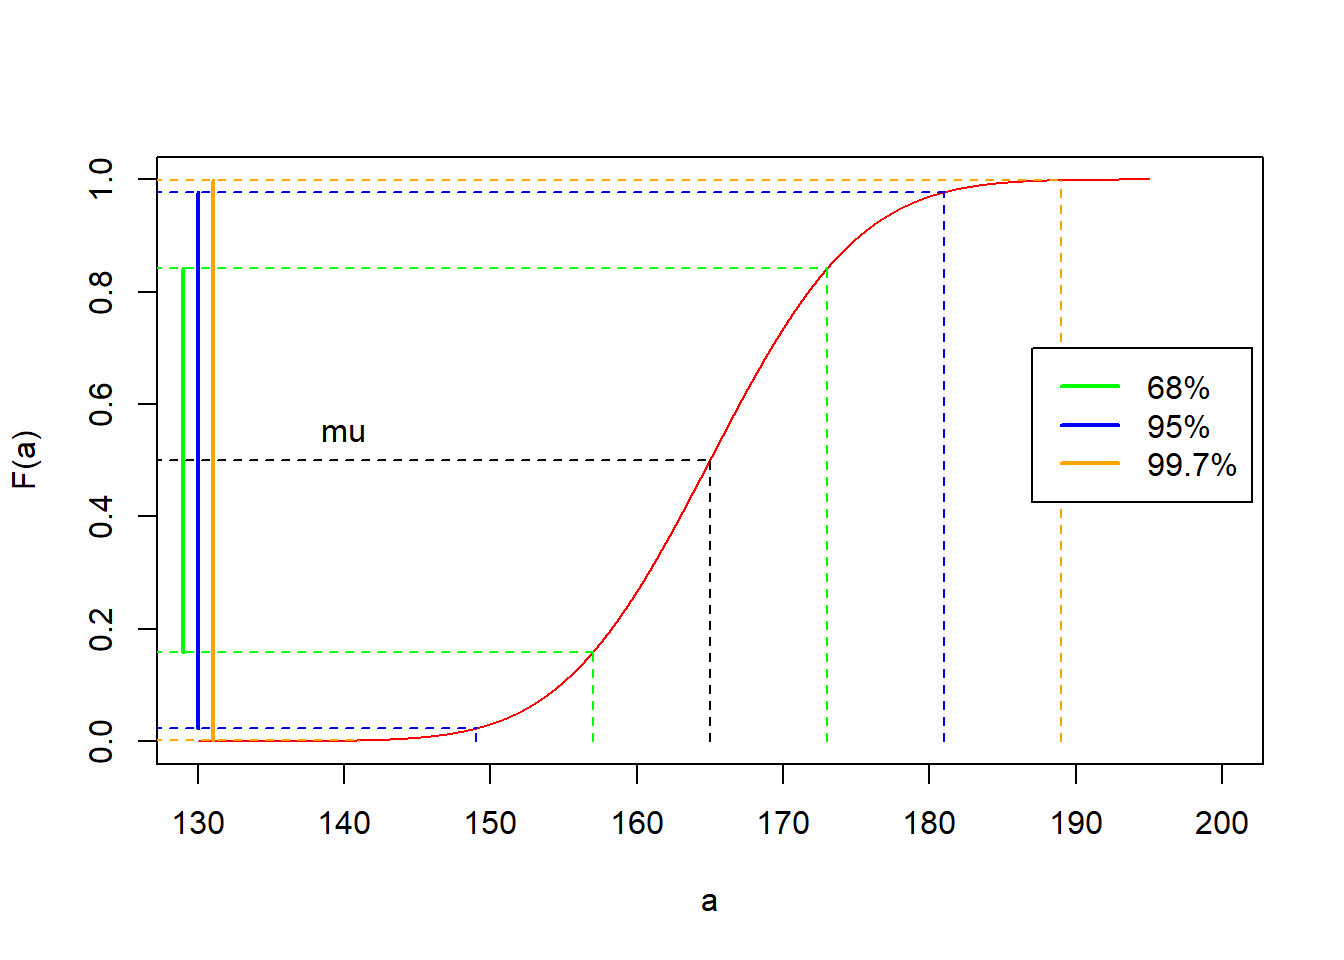
\includegraphics{_main_files/figure-latex/unnamed-chunk-3-1.pdf}

\begin{center}\rule{0.5\linewidth}{0.5pt}\end{center}

\begin{center}\rule{0.5\linewidth}{0.5pt}\end{center}

\hypertarget{gruxe1fico-de-sectores}{%
\section{Gráfico de sectores}\label{gruxe1fico-de-sectores}}

Podemos visualizar las frecuencias relativas con un gráfico de sectores

\begin{itemize}
\tightlist
\item
  Donde el área del círculo representa el 100\% de las observaciones (proporción = 1) y las secciones las frecuencias relativas de todos los resultados.
\end{itemize}

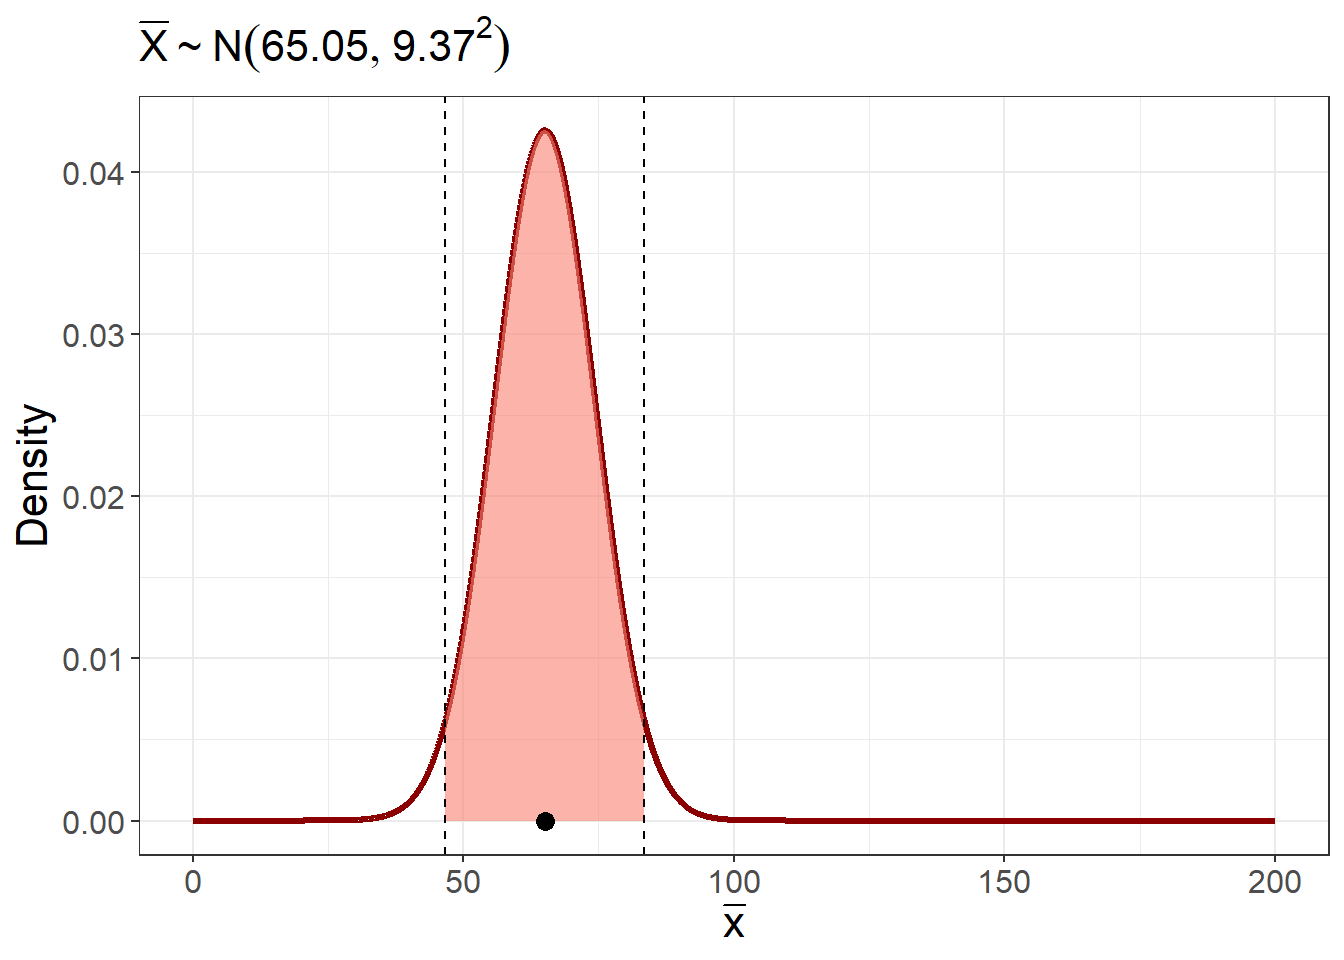
\includegraphics{_main_files/figure-latex/unnamed-chunk-4-1.pdf}

\begin{center}\rule{0.5\linewidth}{0.5pt}\end{center}

\begin{center}\rule{0.5\linewidth}{0.5pt}\end{center}

\hypertarget{variables-categuxf3ricas-y-ordenadas}{%
\section{Variables categóricas y ordenadas}\label{variables-categuxf3ricas-y-ordenadas}}

Los tipos de células no están ordenados de manera lógica en relación con los resultados. Sin embargo, a veces las variables \textbf{categóricas} se pueden \textbf{ordenar}.

Estudio de misofonía:

\begin{itemize}
\item
  123 pacientes fueron examinados por misofonía: ansiedad/ira producida por ciertos sonidos
\item
  Se clasificaron en 4 grupos diferentes según la gravedad.
\end{itemize}

\begin{center}\rule{0.5\linewidth}{0.5pt}\end{center}

\begin{center}\rule{0.5\linewidth}{0.5pt}\end{center}

\hypertarget{ejemplo-2}{%
\section{Ejemplo}\label{ejemplo-2}}

Los resultados del estudio son:

\begin{verbatim}
##   [1] 4 2 0 3 0 0 2 3 0 3 0 2 2 0 2 0 0 3 3 0 3 3 2 0 0 0 4 2 2 0 2 0 0 0 3 0 2
##  [38] 3 2 2 0 2 3 0 0 2 2 3 3 0 0 4 3 3 2 0 2 0 0 0 2 2 0 0 2 3 0 1 3 2 4 3 2 3
##  [75] 0 2 3 2 4 1 2 0 2 0 2 0 2 2 4 3 0 3 0 0 0 2 2 1 3 0 0 3 2 1 3 0 4 4 2 3 3
## [112] 3 0 3 2 1 2 3 3 4 2 3 2
\end{verbatim}

y su tabla de frecuencias

\begin{verbatim}
##   outcome ni         fi
## 1       0 41 0.33333333
## 2       1  5 0.04065041
## 3       2 37 0.30081301
## 4       3 31 0.25203252
## 5       4  9 0.07317073
\end{verbatim}

\begin{center}\rule{0.5\linewidth}{0.5pt}\end{center}

\begin{center}\rule{0.5\linewidth}{0.5pt}\end{center}

\hypertarget{frecuencias-acumuladas-absolutas-y-relativas}{%
\section{Frecuencias acumuladas absolutas y relativas}\label{frecuencias-acumuladas-absolutas-y-relativas}}

La gravedad de la misofonía es \textbf{categórica} y \textbf{ordenada}.

Cuando los resultados se pueden ordenar, entonces es útil preguntarse por el \textbf{número} de observaciones que se obtuvieron hasta un resultado dado. Llamamos a este número la frecuencia acumulada absoluta hasta el resultado \(i\):
\[N_i=\sum_{k=1..i} n_k\]

Tambíen es útil calcular la \textbf{proporción} de las observaciones que se obtuvo hasta un resultado dado

\[F_i=\sum_{k=1..i} f_k\]

\begin{center}\rule{0.5\linewidth}{0.5pt}\end{center}

\begin{center}\rule{0.5\linewidth}{0.5pt}\end{center}

\hypertarget{tabla-de-frecuencia} de los pacientes tenían misofonía hasta la gravedad \textbf{2}
\item
  \textbf{37\%} de los pacientes tienen una gravedad menor o igual a \textbf{1}
\end{itemize}

\begin{center}\rule{0.5\linewidth}{0.5pt}\end{center}

\begin{center}\rule{0.5\linewidth}{0.5pt}\end{center}

\hypertarget{gruxe1fica-de-frecuencia-acumulada}{%
\section{Gráfica de frecuencia acumulada}\label{gruxe1fica-de-frecuencia-acumulada}}

También podemos graficar la frecuencia acumulada Vs los resultados

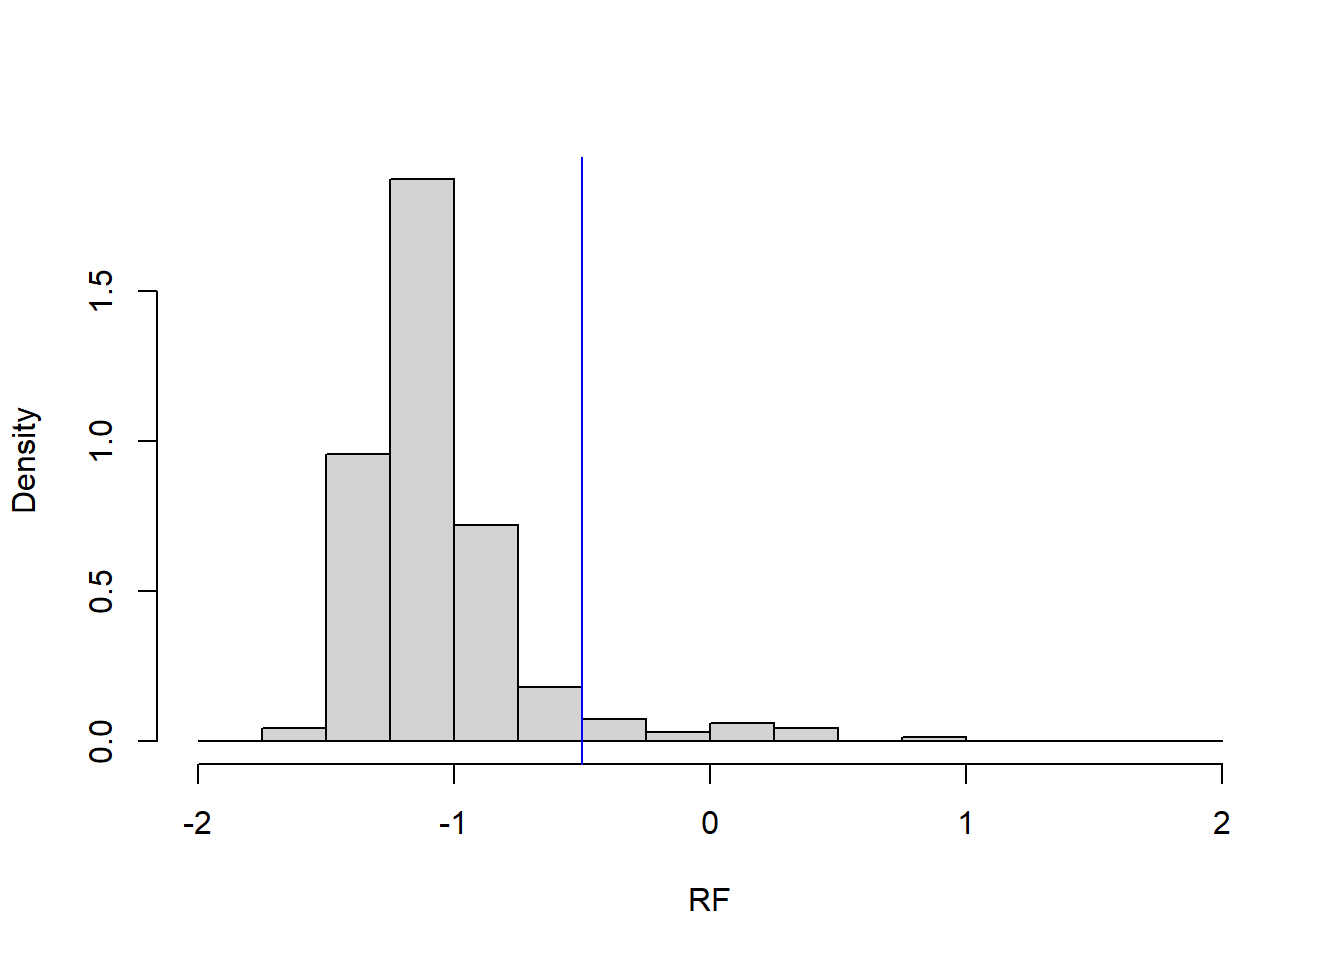
\includegraphics{_main_files/figure-latex/unnamed-chunk-8-1.pdf}
\_\_\_\_\_\_\_\_\_\_\_
\_\_\_\_\_\_\_\_\_\_\_

\hypertarget{variables-continuas}{%
\section{Variables continuas}\label{variables-continuas}}

El resultado de un experimento aleatorio también puede dar resultados continuos.

En el estudio de misofonía, los investigadores se preguntaron si la convexidad de la mandíbula afectaría la gravedad de la misofonía (la hipótesis científica es que el ángulo de convexidad de la mandíbula puede influir en el oído y su sensibilidad). Estos son los resultados para la convexidad de la mandíbula (grados)

\begin{verbatim}
##   [1]  7.97 18.23 12.27  7.81  9.81 13.50 19.30  7.70 12.30  7.90 12.60 19.00
##  [13]  7.27 14.00  5.40  8.00 11.20  7.75  7.94 16.69  7.62  7.02  7.00 19.20
##  [25]  7.96 14.70  7.24  7.80  7.90  4.70  4.40 14.00 14.40 16.00  1.40  9.76
##  [37]  7.90  7.90  7.40  6.30  7.76  7.30  7.00 11.23 16.00  7.90  7.29  6.91
##  [49]  7.10 13.40 11.60 -1.00  6.00  7.82  4.80 11.00  9.00 11.50 16.00 15.00
##  [61]  1.40 16.80  7.70 16.14  7.12 -1.00 17.00  9.26 18.70  3.40 21.30  7.50
##  [73]  6.03  7.50 19.00 19.01  8.10  7.80  6.10 15.26  7.95 18.00  4.60 15.00
##  [85]  7.50  8.00 16.80  8.54  7.00 18.30  7.80 16.00 14.00 12.30 11.40  8.50
##  [97]  7.00  7.96 17.60 10.00  3.50  6.70 17.00 20.26  6.64  1.80  7.02  2.46
## [109] 19.00 17.86  6.10  6.64 12.00  6.60  8.70 14.05  7.20 19.70  7.70  6.02
## [121]  2.50 19.00  6.80
\end{verbatim}

\begin{center}\rule{0.5\linewidth}{0.5pt}\end{center}

\begin{center}\rule{0.5\linewidth}{0.5pt}\end{center}

\hypertarget{contenedores}{%
\section{Contenedores}\label{contenedores}}

¡Los resultados continuos no se pueden contar!

Las transformamos en variables categóricas ordenadas

\begin{itemize}
\tightlist
\item
  Cubrimos el rango de las observaciones en intervalos regulares del mismo tamaño (bins)
\end{itemize}

\begin{verbatim}
## [1] "[-1.02,3.46]" "(3.46,7.92]"  "(7.92,12.4]"  "(12.4,16.8]"  "(16.8,21.3]"
\end{verbatim}

\begin{center}\rule{0.5\linewidth}{0.5pt}\end{center}

\begin{center}\rule{0.5\linewidth}{0.5pt}\end{center}

\hypertarget{crear-una-variable-categuxf3rica-a-partir-de-una-continua}{%
\section{Crear una variable categórica a partir de una continua}\label{crear-una-variable-categuxf3rica-a-partir-de-una-continua}}

\begin{itemize}
\tightlist
\item
  Asignamos cada observación a su intervalo: creando una variable categórica \textbf{ordenada}; en este caso con 5 resultados posibles
\end{itemize}

\begin{verbatim}
##   [1] "(7.92,12.4]"  "(16.8,21.3]"  "(7.92,12.4]"  "(3.46,7.92]"  "(7.92,12.4]" 
##   [6] "(12.4,16.8]"  "(16.8,21.3]"  "(3.46,7.92]"  "(7.92,12.4]"  "(3.46,7.92]" 
##  [11] "(12.4,16.8]"  "(16.8,21.3]"  "(3.46,7.92]"  "(12.4,16.8]"  "(3.46,7.92]" 
##  [16] "(7.92,12.4]"  "(7.92,12.4]"  "(3.46,7.92]"  "(7.92,12.4]"  "(12.4,16.8]" 
##  [21] "(3.46,7.92]"  "(3.46,7.92]"  "(3.46,7.92]"  "(16.8,21.3]"  "(7.92,12.4]" 
##  [26] "(12.4,16.8]"  "(3.46,7.92]"  "(3.46,7.92]"  "(3.46,7.92]"  "(3.46,7.92]" 
##  [31] "(3.46,7.92]"  "(12.4,16.8]"  "(12.4,16.8]"  "(12.4,16.8]"  "[-1.02,3.46]"
##  [36] "(7.92,12.4]"  "(3.46,7.92]"  "(3.46,7.92]"  "(3.46,7.92]"  "(3.46,7.92]" 
##  [41] "(3.46,7.92]"  "(3.46,7.92]"  "(3.46,7.92]"  "(7.92,12.4]"  "(12.4,16.8]" 
##  [46] "(3.46,7.92]"  "(3.46,7.92]"  "(3.46,7.92]"  "(3.46,7.92]"  "(12.4,16.8]" 
##  [51] "(7.92,12.4]"  "[-1.02,3.46]" "(3.46,7.92]"  "(3.46,7.92]"  "(3.46,7.92]" 
##  [56] "(7.92,12.4]"  "(7.92,12.4]"  "(7.92,12.4]"  "(12.4,16.8]"  "(12.4,16.8]" 
##  [61] "[-1.02,3.46]" "(12.4,16.8]"  "(3.46,7.92]"  "(12.4,16.8]"  "(3.46,7.92]" 
##  [66] "[-1.02,3.46]" "(16.8,21.3]"  "(7.92,12.4]"  "(16.8,21.3]"  "[-1.02,3.46]"
##  [71] "(16.8,21.3]"  "(3.46,7.92]"  "(3.46,7.92]"  "(3.46,7.92]"  "(16.8,21.3]" 
##  [76] "(16.8,21.3]"  "(7.92,12.4]"  "(3.46,7.92]"  "(3.46,7.92]"  "(12.4,16.8]" 
##  [81] "(7.92,12.4]"  "(16.8,21.3]"  "(3.46,7.92]"  "(12.4,16.8]"  "(3.46,7.92]" 
##  [86] "(7.92,12.4]"  "(12.4,16.8]"  "(7.92,12.4]"  "(3.46,7.92]"  "(16.8,21.3]" 
##  [91] "(3.46,7.92]"  "(12.4,16.8]"  "(12.4,16.8]"  "(7.92,12.4]"  "(7.92,12.4]" 
##  [96] "(7.92,12.4]"  "(3.46,7.92]"  "(7.92,12.4]"  "(16.8,21.3]"  "(7.92,12.4]" 
## [101] "(3.46,7.92]"  "(3.46,7.92]"  "(16.8,21.3]"  "(16.8,21.3]"  "(3.46,7.92]" 
## [106] "[-1.02,3.46]" "(3.46,7.92]"  "[-1.02,3.46]" "(16.8,21.3]"  "(16.8,21.3]" 
## [111] "(3.46,7.92]"  "(3.46,7.92]"  "(7.92,12.4]"  "(3.46,7.92]"  "(7.92,12.4]" 
## [116] "(12.4,16.8]"  "(3.46,7.92]"  "(16.8,21.3]"  "(3.46,7.92]"  "(3.46,7.92]" 
## [121] "[-1.02,3.46]" "(16.8,21.3]"  "(3.46,7.92]"
\end{verbatim}

\begin{center}\rule{0.5\linewidth}{0.5pt}\end{center}

\begin{center}\rule{0.5\linewidth}{0.5pt}\end{center}

\hypertarget{tabla-de-frecuencias-para-una-variable-continua}{%
\section{Tabla de frecuencias para una variable continua}\label{tabla-de-frecuencias-para-una-variable-continua}}

\begin{verbatim}
##        outcome ni         fi  Ni         Fi
## 1 [-1.02,3.46]  8 0.06504065   8 0.06504065
## 2  (3.46,7.92] 51 0.41463415  59 0.47967480
## 3  (7.92,12.4] 26 0.21138211  85 0.69105691
## 4  (12.4,16.8] 20 0.16260163 105 0.85365854
## 5  (16.8,21.3] 18 0.14634146 123 1.00000000
\end{verbatim}

\begin{center}\rule{0.5\linewidth}{0.5pt}\end{center}

\begin{center}\rule{0.5\linewidth}{0.5pt}\end{center}

\hypertarget{histograma}{%
\section{Histograma}\label{histograma}}

El histograma es la gráfica de \(n_i\) o \(f_i\) Vs los resultados (bins). El histograma depende del tamaño de los contenedores.

\begin{center}\rule{0.5\linewidth}{0.5pt}\end{center}

\begin{center}\rule{0.5\linewidth}{0.5pt}\end{center}

\hypertarget{tabla-de-frecuencias-para-una-variable-continua-1}{%
\section{Tabla de frecuencias para una variable continua}\label{tabla-de-frecuencias-para-una-variable-continua-1}}

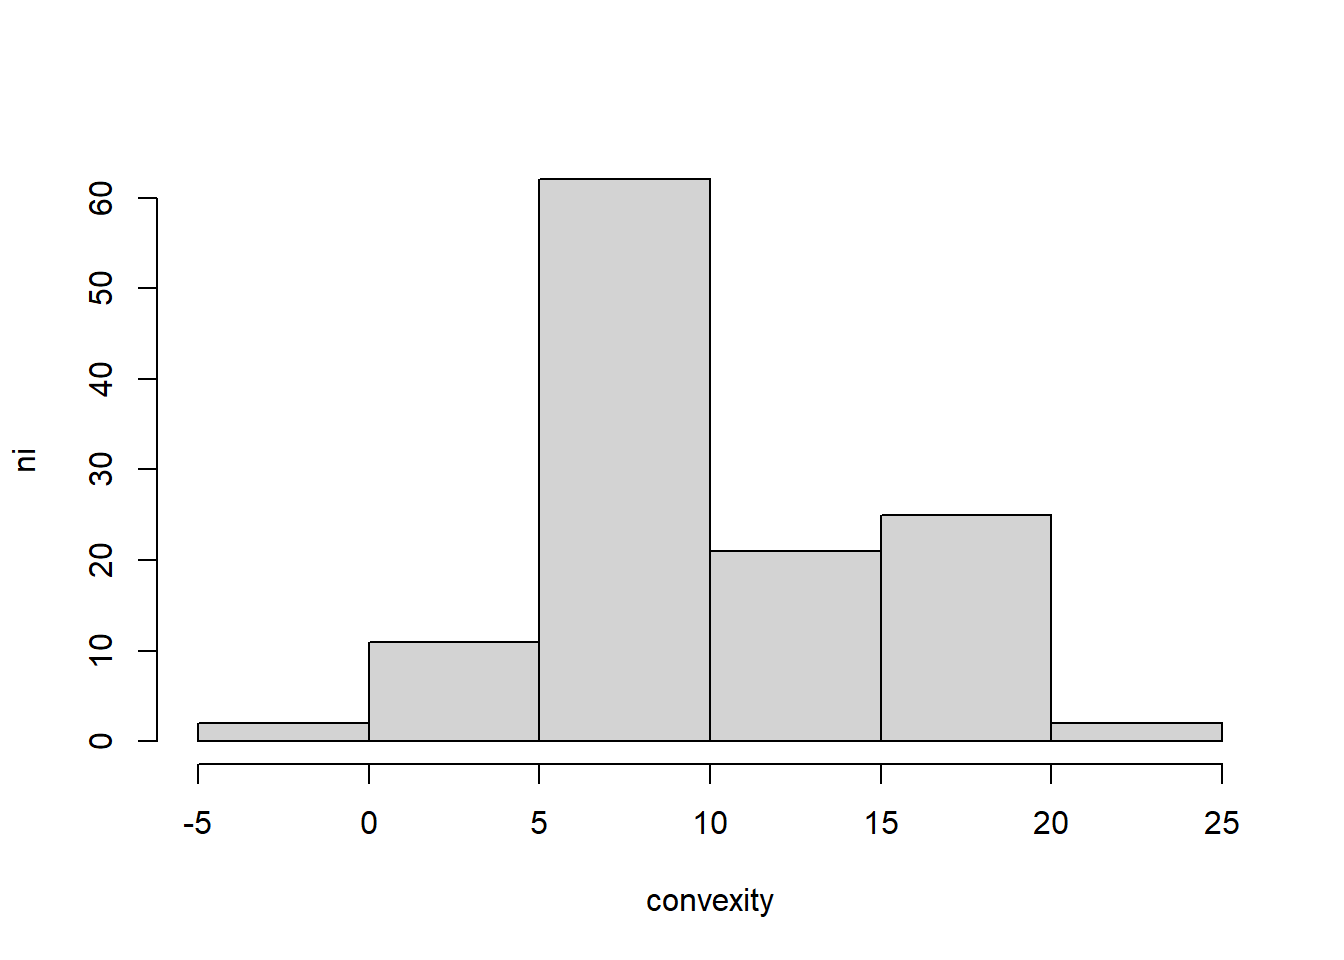
\includegraphics{_main_files/figure-latex/unnamed-chunk-13-1.pdf}

\begin{center}\rule{0.5\linewidth}{0.5pt}\end{center}

\begin{center}\rule{0.5\linewidth}{0.5pt}\end{center}

\hypertarget{histograma-1}{%
\section{Histograma}\label{histograma-1}}

El histograma es la gráfica de \(n_i\) o \(f_i\) Vs los resultados (bins). El histograma depende del tamaño de los contenedores.

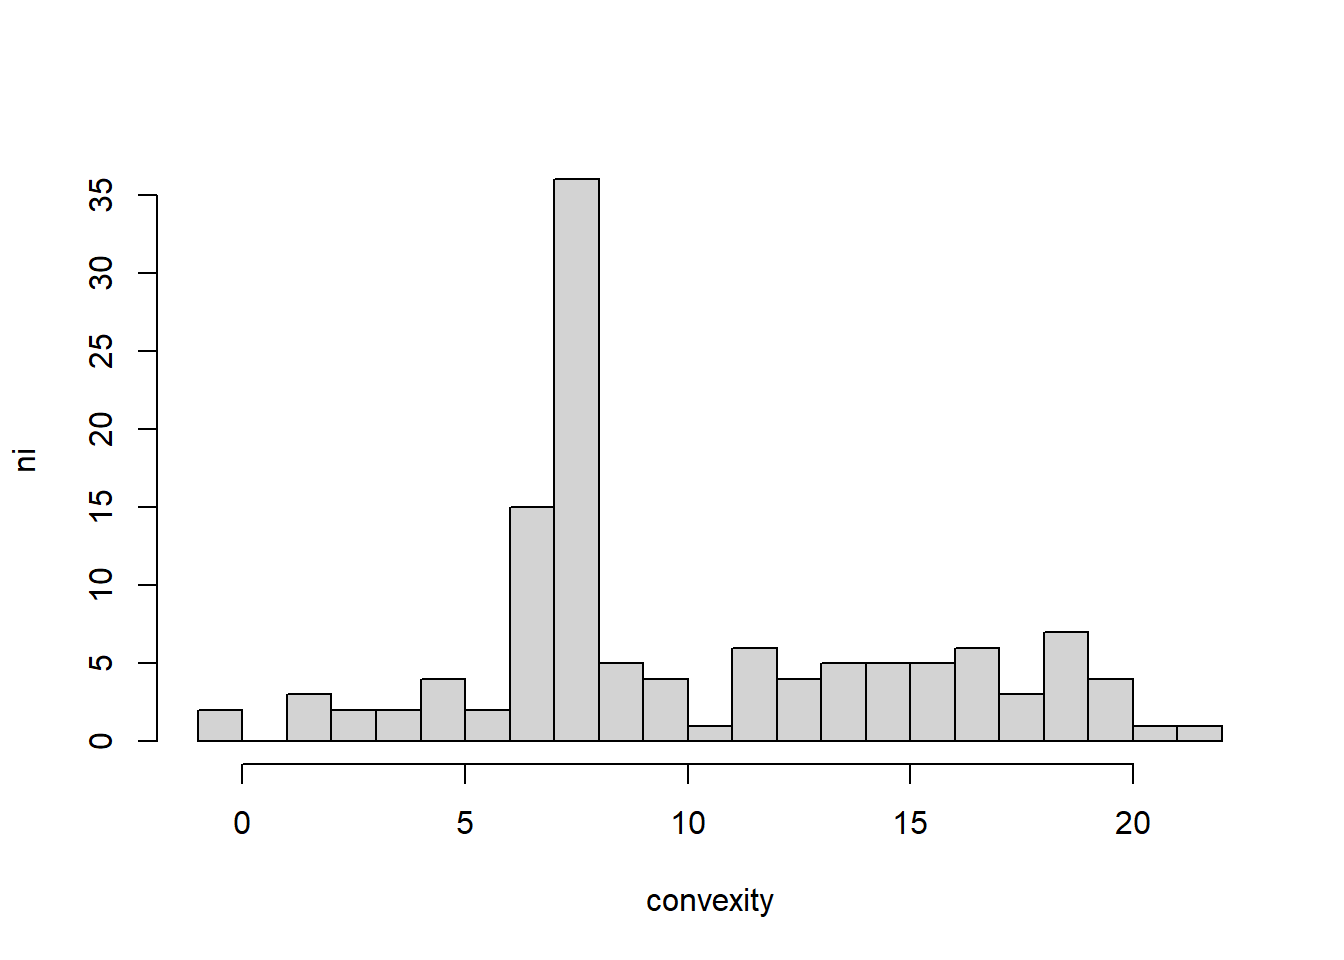
\includegraphics{_main_files/figure-latex/unnamed-chunk-14-1.pdf}

\begin{center}\rule{0.5\linewidth}{0.5pt}\end{center}

\begin{center}\rule{0.5\linewidth}{0.5pt}\end{center}

\hypertarget{gruxe1fica-de-frecuencia-acumulada-variables-continuas}{%
\section{Gráfica de frecuencia acumulada: Variables continuas}\label{gruxe1fica-de-frecuencia-acumulada-variables-continuas}}

También podemos graficar la frecuencia acumulada Vs los resultados

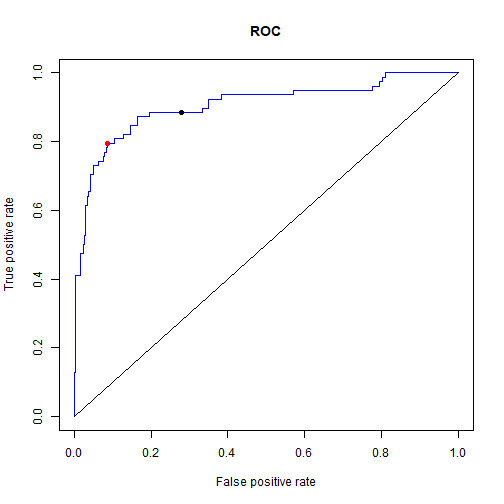
\includegraphics{_main_files/figure-latex/unnamed-chunk-15-1.pdf}

\begin{center}\rule{0.5\linewidth}{0.5pt}\end{center}

\begin{center}\rule{0.5\linewidth}{0.5pt}\end{center}

\hypertarget{resumen-estaduxedstico}{%
\section{Resumen estadístico}\label{resumen-estaduxedstico}}

Las estadísticas de resumen son números calculados a partir de los datos que nos dicen características importantes de las variables numéricas (categóricas o continuas).

Valores límite:

\begin{itemize}
\tightlist
\item
  mínimo: el resultado mínimo observado
\item
  máximo: el resultado máximo observado
\end{itemize}

Valor central para los resultados

\begin{itemize}
\tightlist
\item
  El promedio se define como
\end{itemize}

\[\bar{x}=\frac{1}{N} \sum_{j=1..N} x_j\]

donde \(x_j\) es la \textbf{observación} \(j\) (convexidad) de un total de \(N\).

\begin{center}\rule{0.5\linewidth}{0.5pt}\end{center}

\begin{center}\rule{0.5\linewidth}{0.5pt}\end{center}

\hypertarget{promedio}{%
\section{Promedio}\label{promedio}}

La convexidad promedio se puede calcular directamente a partir de las \textbf{observaciones}

\(\bar{x}= \frac{1}{N}\sum_j x_j\)

\(= \frac{1}{N}(7.97 + 18.23 + 12.27... + 6.80) = 10.19894\)

\begin{center}\rule{0.5\linewidth}{0.5pt}\end{center}

\begin{center}\rule{0.5\linewidth}{0.5pt}\end{center}

\hypertarget{promedio-ordenado-categuxf3ricamente}{%
\section{Promedio (ordenado categóricamente)}\label{promedio-ordenado-categuxf3ricamente}}

Para las variables \textbf{ordenadas categóricamente}, podemos usar la tabla de frecuencias para calcular el promedio

\begin{verbatim}
##   outcome ni         fi
## 1       0 41 0.33333333
## 2       1  5 0.04065041
## 3       2 37 0.30081301
## 4       3 31 0.25203252
## 5       4  9 0.07317073
\end{verbatim}

La \textbf{severidad} promedio de la misofonía en el estudio
\textbf{también} puede calcularse a partir de las frecuencias relativas de los \textbf{resultados}

\(\bar{x}=\frac{1}{N}\sum_{i=1...N} x_j=\frac{1}{N}\sum_{i=1...M} x_i*n_ {i}=\sum_{i=1...M} x_i*f_{i}\)

\(=0*f_{0}+1*f_{1}+2*f_{2}+3*f_{3}+4*f_{4}=1,691057\)

(note el cambio de \(N\) a \(M\) en la segunda suma)

\begin{center}\rule{0.5\linewidth}{0.5pt}\end{center}

\begin{center}\rule{0.5\linewidth}{0.5pt}\end{center}

\hypertarget{promedio-ordenado-categuxf3ricamente-1}{%
\section{Promedio (ordenado categóricamente)}\label{promedio-ordenado-categuxf3ricamente-1}}

En términos de los \textbf{resultados} de las variables ordenadas categóricas, el \textbf{promedio} se puede escribir como

\[\bar{x}= \sum_{i = 1...M} x_i f_i\]

de un total de \(M\) posibles resultados (número de niveles de gravedad).

\(\bar{x}\) es el \textbf{valor central} o centro de gravedad de los resultados. Como si cada resultado tuviera una densidad de masa dada por \(f_i\).

\begin{center}\rule{0.5\linewidth}{0.5pt}\end{center}

\begin{center}\rule{0.5\linewidth}{0.5pt}\end{center}

\hypertarget{promedio-1}{%
\section{Promedio}\label{promedio-1}}

\begin{itemize}
\item
  El promedio no es el resultado de una observación (experimento aleatorio).
\item
  Es el resultado de una serie de observaciones (muestra).
\item
  Describe el número donde se equilibran los valores observados.
\end{itemize}

Por eso escuchamos, por ejemplo, que un paciente con una infección puede contagiar a una media de 2,5 personas.

\begin{center}\rule{0.5\linewidth}{0.5pt}\end{center}

\begin{center}\rule{0.5\linewidth}{0.5pt}\end{center}

\hypertarget{promedio-2}{%
\section{Promedio}\label{promedio-2}}

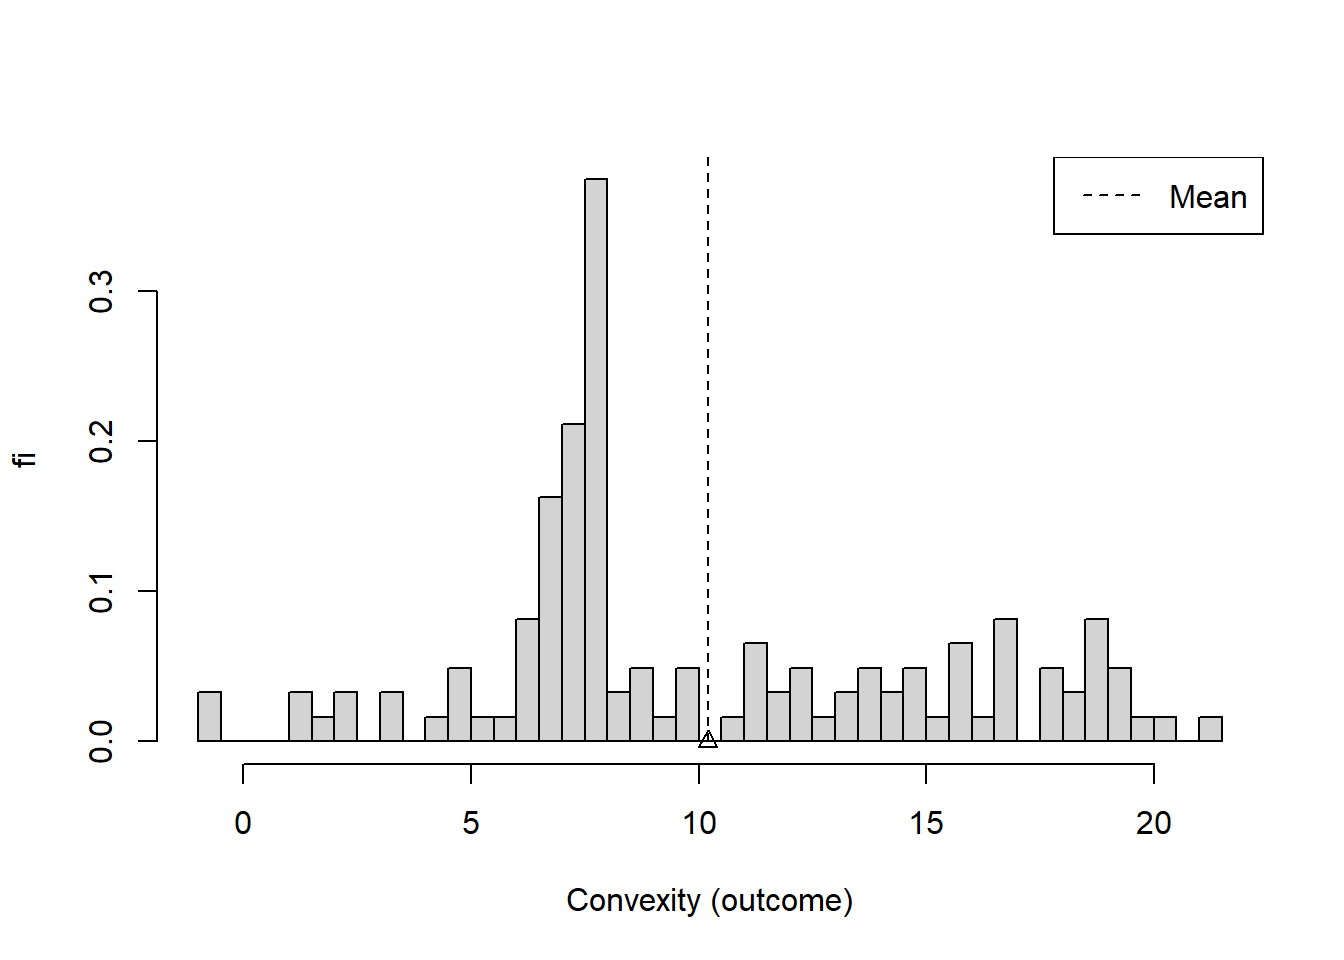
\includegraphics{_main_files/figure-latex/unnamed-chunk-17-1.pdf}

\begin{center}\rule{0.5\linewidth}{0.5pt}\end{center}

\begin{center}\rule{0.5\linewidth}{0.5pt}\end{center}

\hypertarget{mediana}{%
\section{mediana}\label{mediana}}

Otra medida de centralidad es la mediana. La mediana \(q_{0.5}\) es el valor \(x_p\)

\[mediana(x)=q_{0.5}=x_p\]

debajo del cual encontramos la mitad de las observaciones

\[\sum_{x\leq x_p} 1 = \frac{N}{2}\]

o en términos de frecuencias, es el valor \(x_p\) que hace que la frecuencia acumulada \(F_p\) sea igual a \(0.5\)

\[q_{0.5}=\sum_{x\leq x_p} f_x =F_p=0.5\]

\begin{center}\rule{0.5\linewidth}{0.5pt}\end{center}

\begin{center}\rule{0.5\linewidth}{0.5pt}\end{center}

\hypertarget{mediana-vs-promedio}{%
\section{Mediana Vs Promedio}\label{mediana-vs-promedio}}

\begin{itemize}
\tightlist
\item
  Promedio: Centro de masa (compensa valores distantes)
\item
  Mediana: La mitad de la masa
\end{itemize}

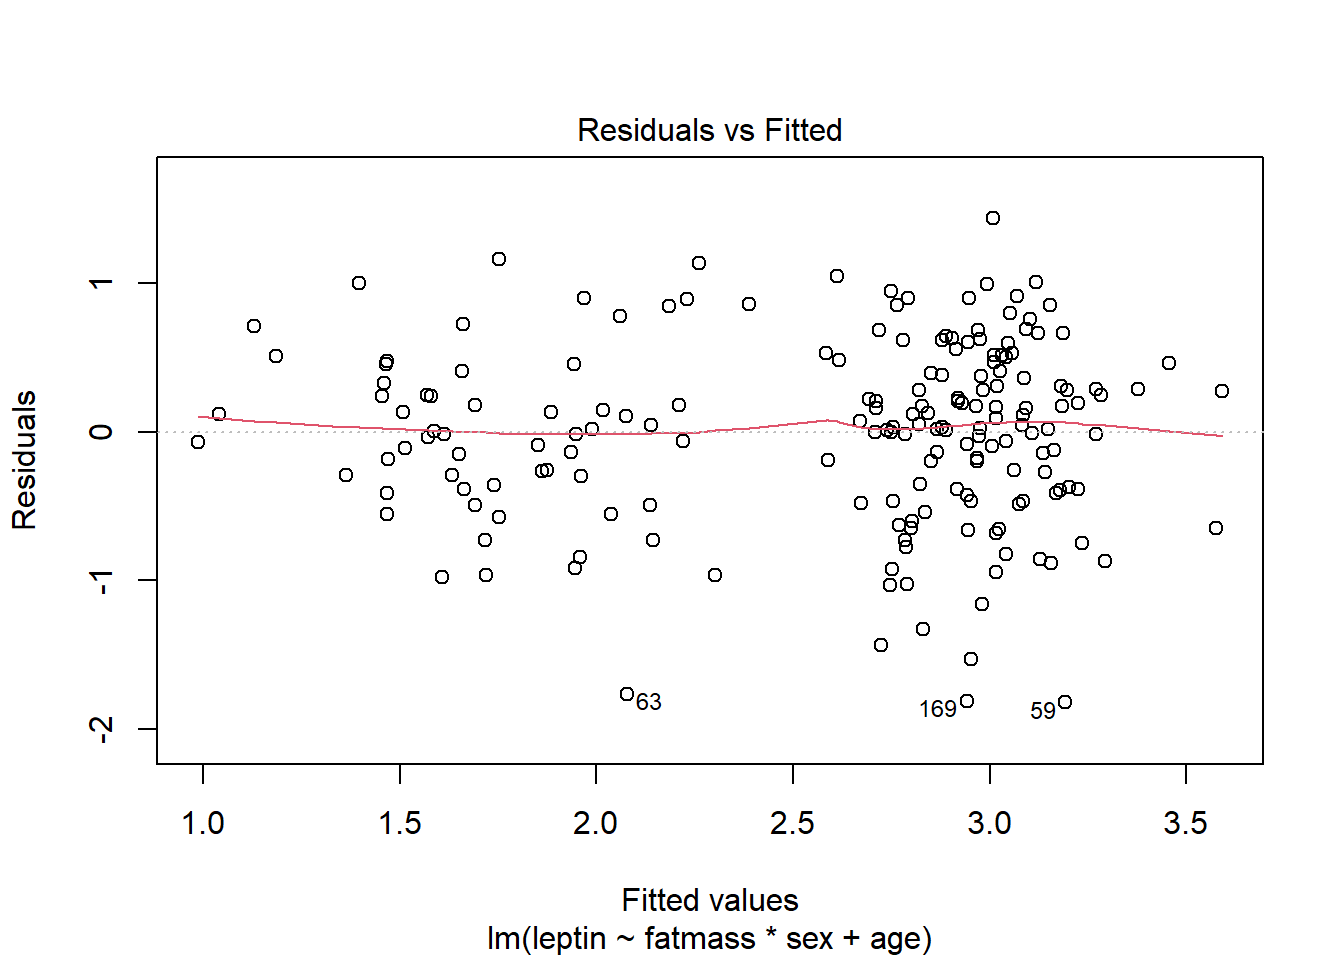
\includegraphics{_main_files/figure-latex/unnamed-chunk-18-1.pdf}

\begin{center}\rule{0.5\linewidth}{0.5pt}\end{center}

\begin{center}\rule{0.5\linewidth}{0.5pt}\end{center}

\hypertarget{dispersiuxf3n}{%
\section{Dispersión}\label{dispersiuxf3n}}

Una medida importante de los resultados es su \textbf{dispersión}. Muchos experimentos pueden compartir su media, pero difieren en la dispersión de los valores.

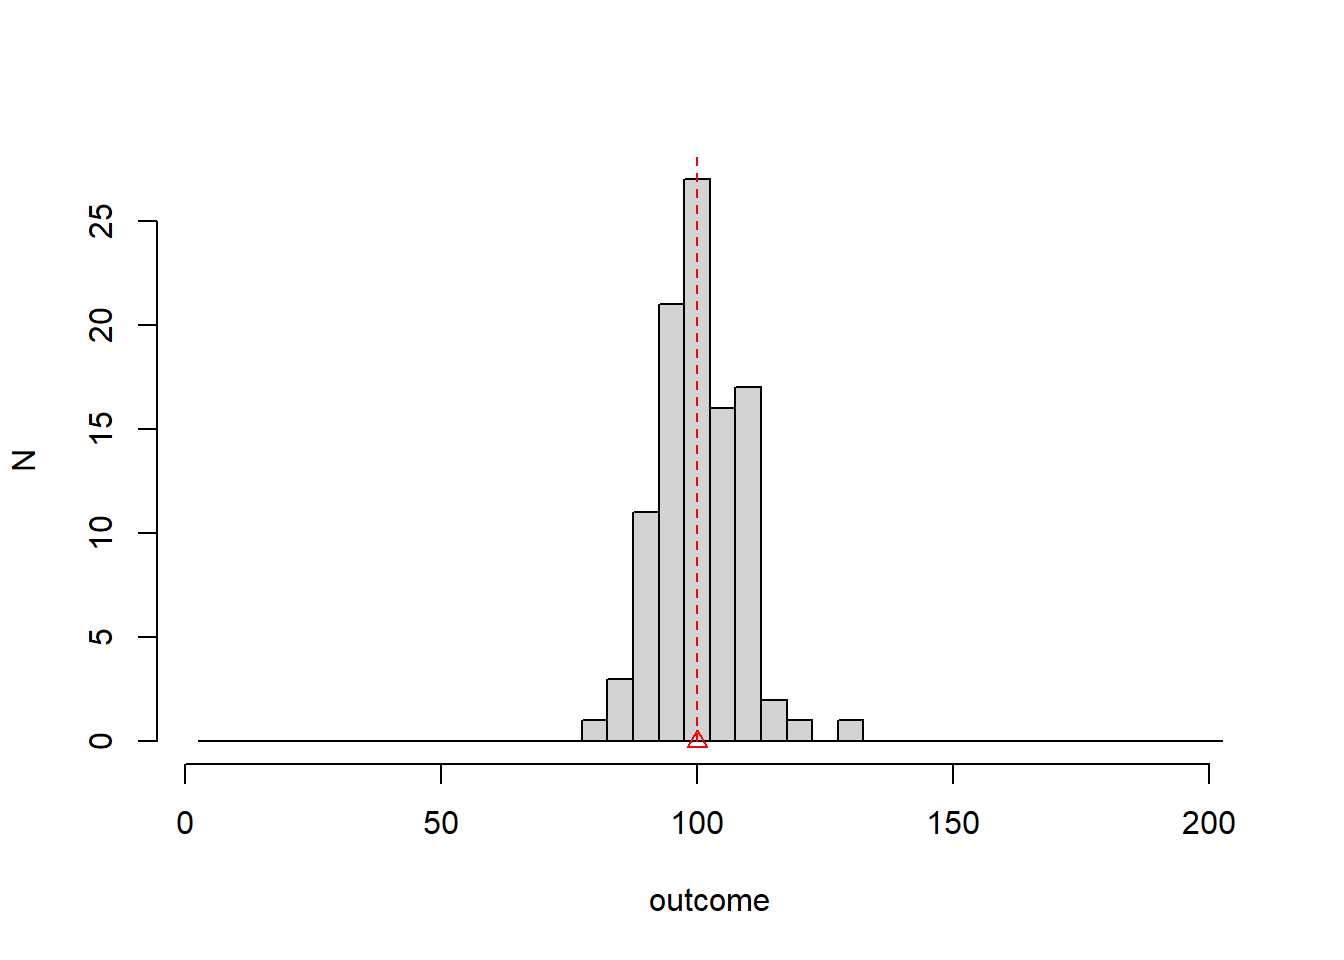
\includegraphics{_main_files/figure-latex/unnamed-chunk-19-1.pdf}

\begin{center}\rule{0.5\linewidth}{0.5pt}\end{center}

\begin{center}\rule{0.5\linewidth}{0.5pt}\end{center}

\hypertarget{dispersiuxf3n-1}{%
\section{Dispersión}\label{dispersiuxf3n-1}}

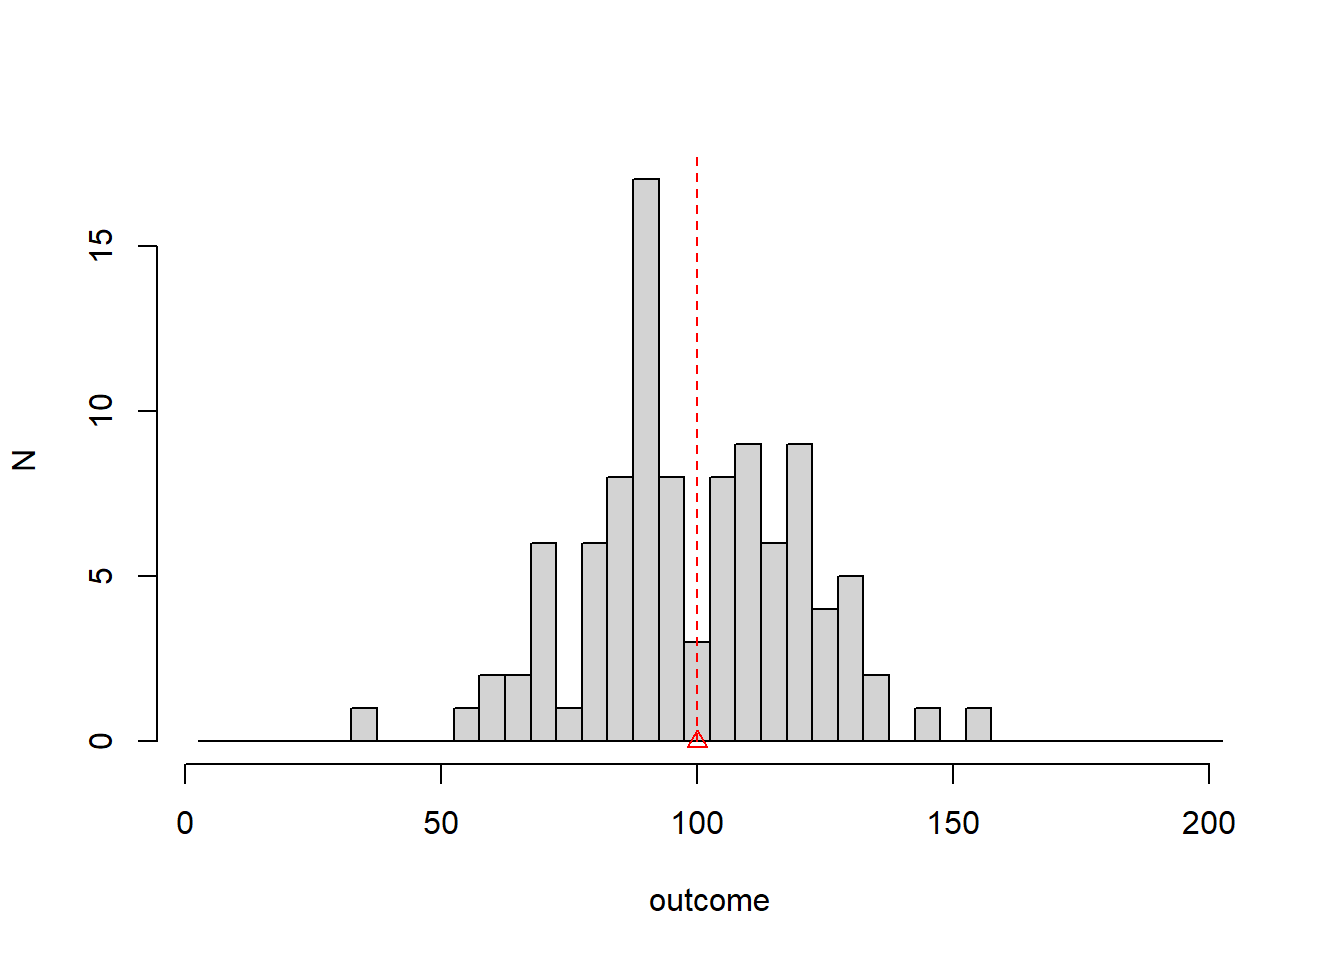
\includegraphics{_main_files/figure-latex/unnamed-chunk-20-1.pdf}

\begin{center}\rule{0.5\linewidth}{0.5pt}\end{center}

\begin{center}\rule{0.5\linewidth}{0.5pt}\end{center}

\hypertarget{variaciuxf3n-de-la-muestra}{%
\section{Variación de la muestra}\label{variaciuxf3n-de-la-muestra}}

La dispersión con respecto a la media se mide con el

\begin{itemize}
\tightlist
\item
  La varianza muestral:
\end{itemize}

\[s^2=\frac{1}{N-1} \sum_{j=1..N} (x_j-\bar{x})^2\]

Mide la distancia cuadrada promedio de las \textbf{observaciones} al promedio. La razón de \(N-1\) se explicará cuando hablemos de inferencia.

\begin{center}\rule{0.5\linewidth}{0.5pt}\end{center}

\begin{center}\rule{0.5\linewidth}{0.5pt}\end{center}

\hypertarget{variaciuxf3n-de-la-muestra-1}{%
\section{Variación de la muestra}\label{variaciuxf3n-de-la-muestra-1}}

\begin{itemize}
\tightlist
\item
  En términos de frecuencias de variables \textbf{categóricas y ordenadas}
\end{itemize}

\[s^2=\frac{N}{N-1} \sum_{x} (x-\bar{x})^2 f_x\]

\(s^2\) se puede considerar como el momento de inercia de las observaciones.

\begin{center}\rule{0.5\linewidth}{0.5pt}\end{center}

\begin{center}\rule{0.5\linewidth}{0.5pt}\end{center}

\hypertarget{desviaciuxf3n-estuxe1ndar}{%
\section{Desviación Estándar}\label{desviaciuxf3n-estuxe1ndar}}

La raíz cuadrada de la varianza de la muestra se denomina \textbf{desviación estándar} \(s\).

La desviación estándar del ángulo de convexidad es

\(s= [\frac{1}{123-1}((7,97-10,19894)^2+ (18,23-10,19894)^2\)
\(+ (12,27-10,19894)^2 + ...)]^{1/2} = 5,086707\)

La convexidad de la mandíbula se desvía de su media en \(5,086707\).

\begin{center}\rule{0.5\linewidth}{0.5pt}\end{center}

\begin{center}\rule{0.5\linewidth}{0.5pt}\end{center}

\hypertarget{ric}{%
\section{RIC}\label{ric}}

\begin{itemize}
\item
  La dispersión de datos también se puede medir con respecto a la mediana por el \textbf{rango intercuartílico}
\item
  Definimos el \textbf{primer} cuartil como el valor \(x_p\) que hace que la frecuencia acumulada \(F_p\) sea igual a \(0,25\)
\end{itemize}

\[q_{0.25}=\sum_{x\leq x_p} f_x =F_p=0.25\]

\begin{itemize}
\tightlist
\item
  También definimos el \textbf{tercer} cuartil como el valor \(x_p\) que hace que la frecuencia acumulada \(F_p\) sea igual a \(0,75\)
\end{itemize}

\[q_{0.75}=\sum_{x\leq x_p} f_x =F_p=0.75\]

\begin{center}\rule{0.5\linewidth}{0.5pt}\end{center}

\begin{center}\rule{0.5\linewidth}{0.5pt}\end{center}

\hypertarget{ric-1}{%
\section{RIC}\label{ric-1}}

La distancia entre el tercer cuartil y el primer cuartil se denomina \textbf{rango intercuartílico} (RIC) y captura el 50 \% central de las observaciones

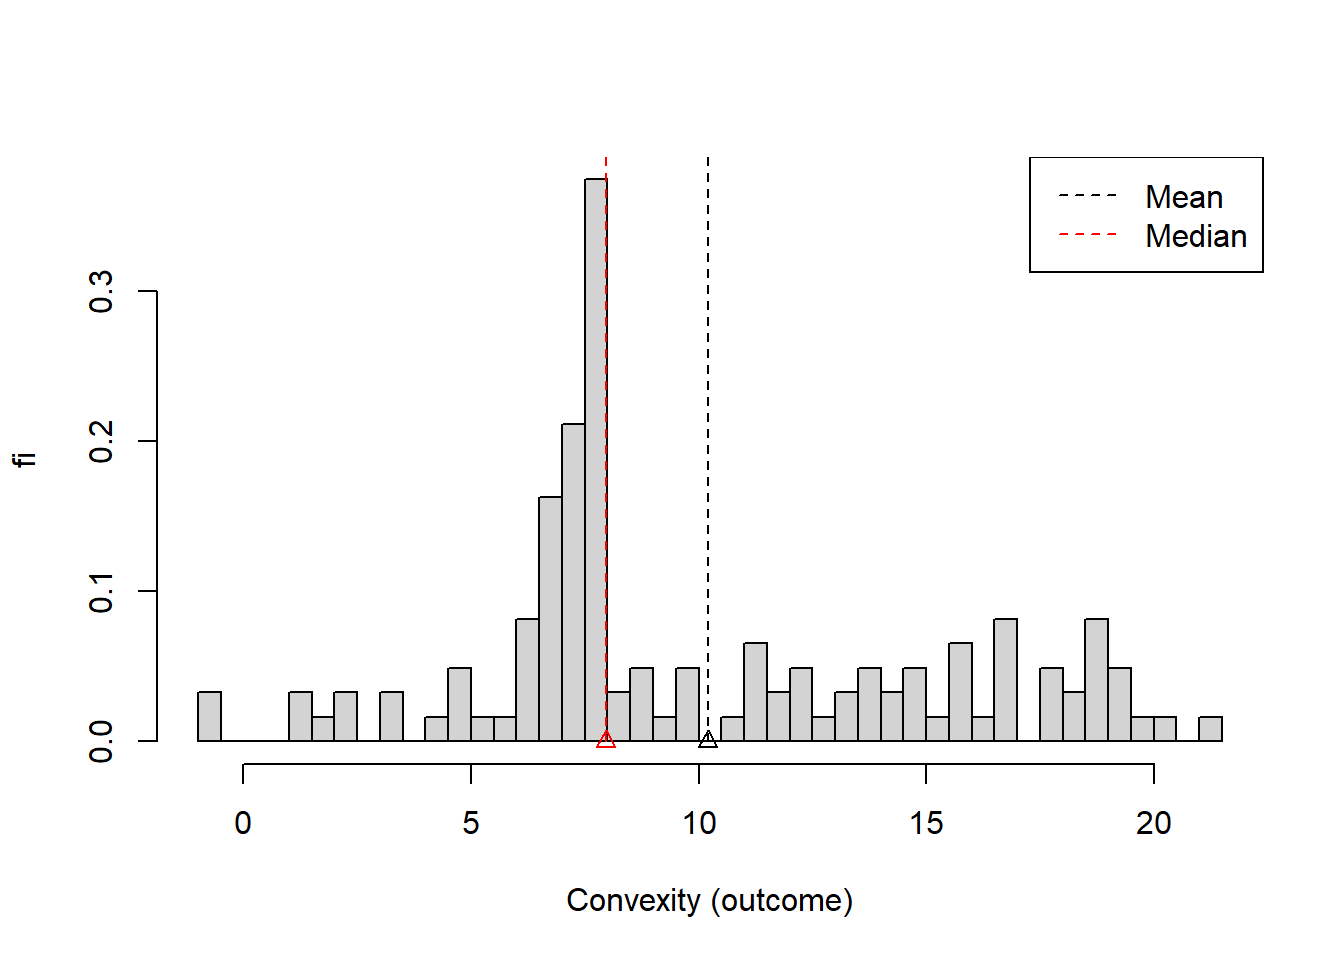
\includegraphics{_main_files/figure-latex/unnamed-chunk-21-1.pdf}

\begin{center}\rule{0.5\linewidth}{0.5pt}\end{center}

\begin{center}\rule{0.5\linewidth}{0.5pt}\end{center}

\hypertarget{diagrama-de-caja}{%
\section{Diagrama de caja}\label{diagrama-de-caja}}

El rango intercuartílico, la mediana y el 5 \% y el 95 \% de los datos se pueden visualizar en un \textbf{diagrama de caja}, aquí los valores de los resultados están en el eje y. El IQR es la caja, la mediana es la línea del medio y los bigotes marcan el 5\% y el 95\% de los datos.

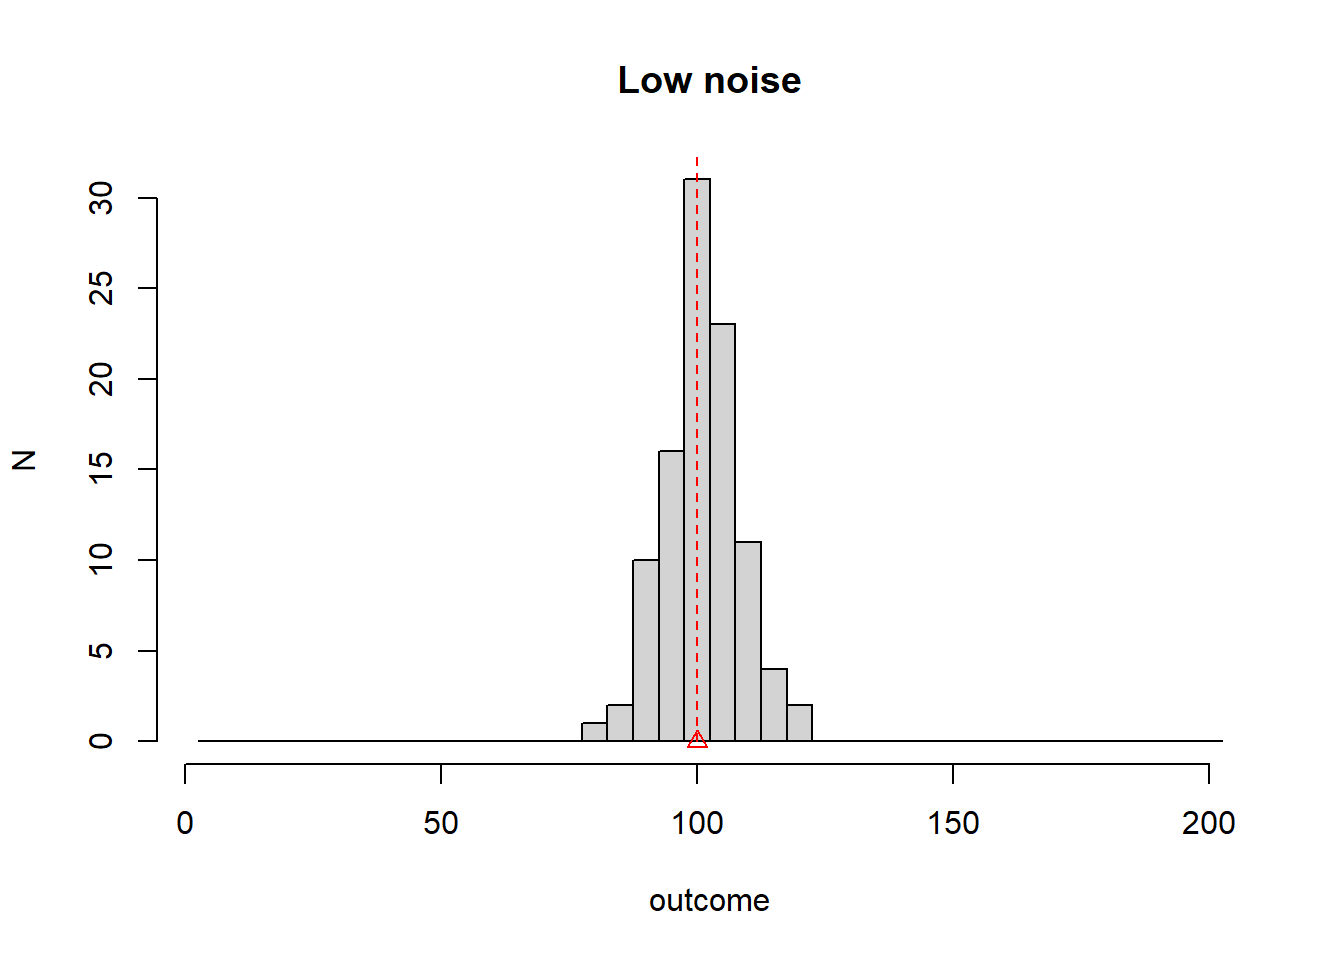
\includegraphics{_main_files/figure-latex/unnamed-chunk-22-1.pdf}

\hypertarget{probabilidad}{%
\chapter{Probabilidad}\label{probabilidad}}

\hypertarget{objetivo-2}{%
\section{Objetivo}\label{objetivo-2}}

\begin{itemize}
\tightlist
\item
  Definición de probabilidad
\item
  Álgebra de probabilidad
\item
  Probabilidad conjunta
\end{itemize}

\begin{center}\rule{0.5\linewidth}{0.5pt}\end{center}

\begin{center}\rule{0.5\linewidth}{0.5pt}\end{center}

\hypertarget{experimentos-aleatorios-1}{%
\section{Experimentos aleatorios}\label{experimentos-aleatorios-1}}

\textbf{Observación}

\begin{itemize}
\tightlist
\item
  y \textbf{observación} es la adquisición de un número o una característica de un experimento
\end{itemize}

\textbf{Salir}

\begin{itemize}
\tightlist
\item
  Un \textbf{resultado} es una posible observación que es el resultado de un experimento.
\end{itemize}

\textbf{Experimento aleatorio}

\begin{itemize}
\tightlist
\item
  Un experimento que da resultados \textbf{diferentes} cuando se repite de la misma manera.
\end{itemize}

\begin{center}\rule{0.5\linewidth}{0.5pt}\end{center}

\begin{center}\rule{0.5\linewidth}{0.5pt}\end{center}

\hypertarget{probabilidad-1}{%
\section{Probabilidad}\label{probabilidad-1}}

La \textbf{probabilidad} de un resultado es una medida de cuán seguros estamos de observar ese resultado al realizar un experimento aleatorio.

\begin{itemize}
\item
  0: Estamos seguros de que la observación \textbf{no} ocurrirá.
\item
  1: Estamos seguros de que la observación sucederá.
\end{itemize}

\begin{center}\rule{0.5\linewidth}{0.5pt}\end{center}

\begin{center}\rule{0.5\linewidth}{0.5pt}\end{center}

\hypertarget{ejemplo-3}{%
\section{Ejemplo}\label{ejemplo-3}}

\begin{itemize}
\tightlist
\item
  Considere las siguientes observaciones de un experimento aleatorio:
\end{itemize}

1 5 1 2 2 1 2 2

\begin{itemize}
\tightlist
\item
  ¿Qué tan seguro estamos de obtener \(2\) en la siguiente observación?
\end{itemize}

\begin{center}\rule{0.5\linewidth}{0.5pt}\end{center}

\begin{center}\rule{0.5\linewidth}{0.5pt}\end{center}

\hypertarget{ejemplo-4}{%
\section{Ejemplo}\label{ejemplo-4}}

La tabla de frecuencias es

\begin{verbatim}
##   outcome ni    fi
## 1       1  3 0.375
## 2       2  4 0.500
## 3       5  1 0.125
\end{verbatim}

La \textbf{frecuencia relativa} \(f_i\)

\begin{itemize}
\tightlist
\item
  es un número entre \(0\) y \(1\).
\item
  mide la proporción del total de observaciones que observamos un resultado particular.
\item
  parece una medida de probabilidad razonable.
\end{itemize}

Como \(f_2=0.5\) entonces estaríamos \(50º%
\) seguros de obtener \(2\) en la siguiente repetición del experimento.

\begin{center}\rule{0.5\linewidth}{0.5pt}\end{center}

\begin{center}\rule{0.5\linewidth}{0.5pt}\end{center}

\hypertarget{frecuencia-relativa}{%
\section{Frecuencia relativa}\label{frecuencia-relativa}}

¿\(f_i\) es una buena medida de certeza?

Digamos que repetimos el experimento 12 veces más:

1 5 1 2 2 1 2 2 \textbf{3 1 1 3 3 1 6 3 5 6 4 4}

La tabla de frecuencias es ahora

\begin{verbatim}
##   outcome ni  fi
## 1       1  6 0.3
## 2       2  4 0.2
## 3       3  4 0.2
## 4       4  2 0.1
## 5       5  2 0.1
## 6       6  2 0.1
\end{verbatim}

Aparecieron nuevos resultados y \(f_2\) ahora es \(0.2\), ahora estamos un \(20\%\) seguros de obtener \(2\) en el próximo experimento\ldots{} la probabilidad no debería depender de \(N\)

\begin{center}\rule{0.5\linewidth}{0.5pt}\end{center}

\begin{center}\rule{0.5\linewidth}{0.5pt}\end{center}

\hypertarget{en-el-infinito}{%
\section{En el infinito}\label{en-el-infinito}}

Digamos que repetimos el experimento 1000 veces:

\begin{verbatim}
##   outcome  ni    fi
## 1       1 163 0.163
## 2       2 149 0.149
## 3       3 155 0.155
## 4       4 198 0.198
## 5       5 174 0.174
## 6       6 161 0.161
\end{verbatim}

Encontramos que \(f_i\) está convergiendo a un valor constante

\[lim_{N\rightarrow \infty} f_i = P_i\]

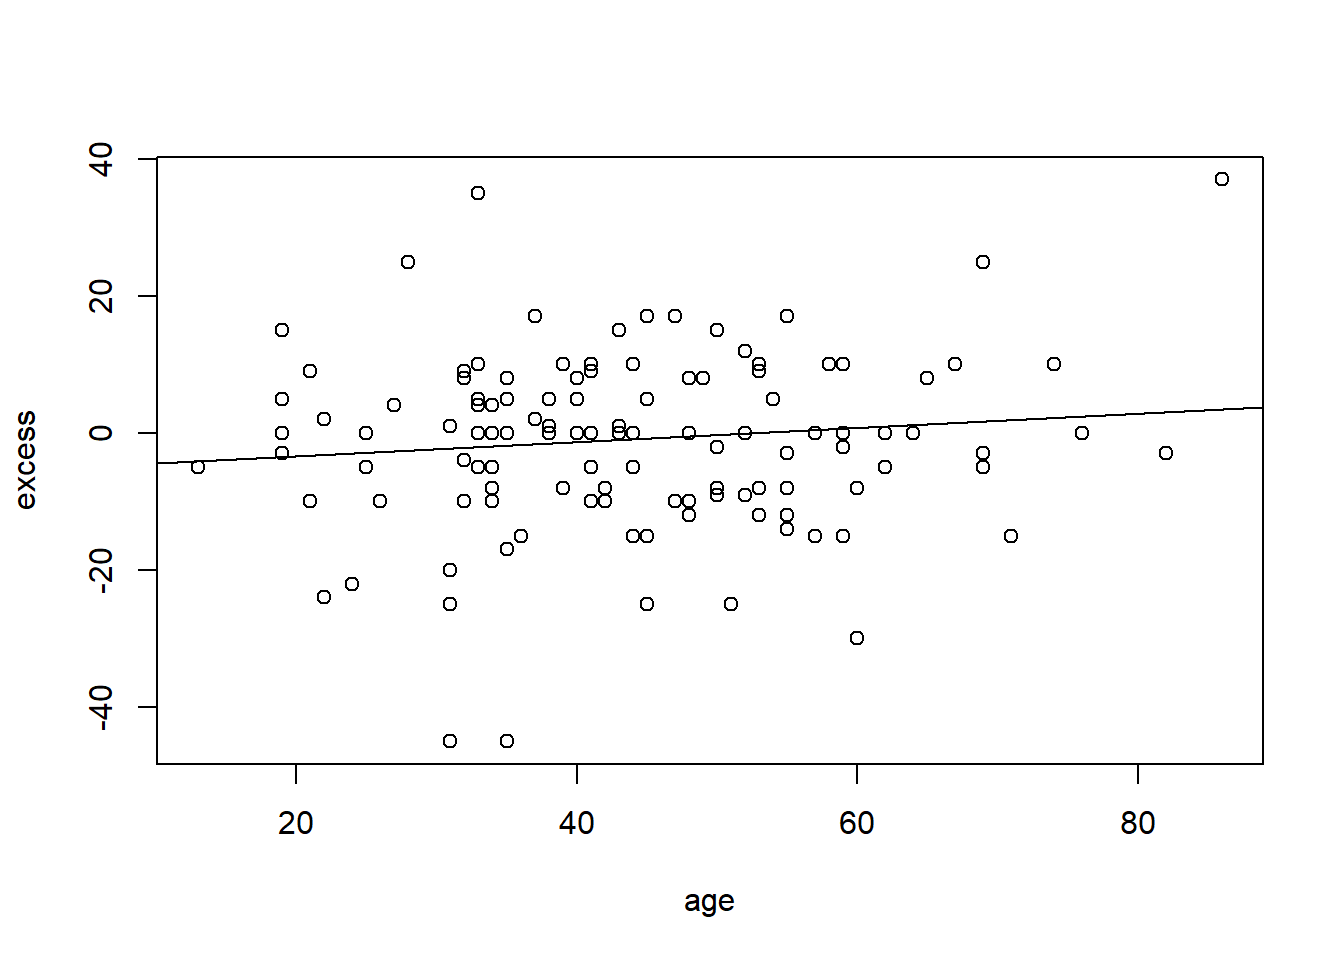
\includegraphics{_main_files/figure-latex/unnamed-chunk-26-1.pdf}

\begin{center}\rule{0.5\linewidth}{0.5pt}\end{center}

\begin{center}\rule{0.5\linewidth}{0.5pt}\end{center}

\hypertarget{probabilidad-frecuentista}{%
\section{Probabilidad frecuentista}\label{probabilidad-frecuentista}}

Llamamos \textbf{Probabilidad} \(P_i\) al límite cuando \(N \rightarrow \infty\) de la \textbf{frecuencia relativa} de observar el resultado \(i\) en un experimento aleatorio.

Defendida por \href{https://plato.stanford.edu/entries/probability-interpret/\#ClaPro}{Venn (1876)}

La interpretación frecuentista de probabilidades se deriva de datos/experiencia (empírica).

\begin{itemize}
\tightlist
\item
  No observamos \(P_i\), observamos \(f_i\)
\item
  Cuando \textbf{estimamos} \(P_i\) con \(f_i\) (normalmente cuando \(N\) es grande), escribimos: \[\hat{P_i}=f_i\]
\end{itemize}

\begin{center}\rule{0.5\linewidth}{0.5pt}\end{center}

\begin{center}\rule{0.5\linewidth}{0.5pt}\end{center}

\hypertarget{probabilidad-cluxe1sica}{%
\section{Probabilidad clásica}\label{probabilidad-cluxe1sica}}

Cada vez que un experimento aleatorio tiene \(M\) resultados posibles que son todos \textbf{igualmente probables}, la probabilidad de cada resultado es \(\frac{1}{M}\).

Defendida por \href{https://plato.stanford.edu/entries/probability-interpret/\#ClaPro}{Laplace (1814)}.

Dado que cada resultado es \textbf{igualmente probable}, declaramos una completa ignorancia y lo mejor que podemos hacer es distribuir equitativamente la misma probabilidad para cada resultado.

¿Y si te dijera que nuestro experimento fue tirar un dado? entonces

\(P_2=1/6=0.166666\).

\[P_i=lim_{N\rightarrow \infty} \frac{n_i}{N}=\frac{1}{M}\]

\begin{center}\rule{0.5\linewidth}{0.5pt}\end{center}

\begin{center}\rule{0.5\linewidth}{0.5pt}\end{center}

\hypertarget{probabilidades-cluxe1sicas-y-frecuentistas}{%
\section{Probabilidades clásicas y frecuentistas}\label{probabilidades-cluxe1sicas-y-frecuentistas}}

\begin{center}\rule{0.5\linewidth}{0.5pt}\end{center}

\begin{center}\rule{0.5\linewidth}{0.5pt}\end{center}

\hypertarget{probabilidad-2}{%
\section{Probabilidad}\label{probabilidad-2}}

La probabilidad es un número entre \(0\) y \(1\) que se asigna a cada miembro \(E\) de una colección de \textbf{eventos} de un \textbf{espacio muestral} (\(S\)) de un experimento aleatorio.

\[P(E) \in (0,1)\]

donde \(E \in S\)

\begin{center}\rule{0.5\linewidth}{0.5pt}\end{center}

\begin{center}\rule{0.5\linewidth}{0.5pt}\end{center}

\hypertarget{espacio-muestral}{%
\section{Espacio muestral}\label{espacio-muestral}}

Empezamos razonando cuáles son todos los valores posibles (resultados) que podría dar un experimento aleatorio.

Tenga en cuenta que no tenemos que observarlos en un experimento en particular: estamos usando \textbf{razón/lógica} y no observación.

\textbf{Definición:}

\begin{itemize}
\item
  El conjunto de todos los resultados posibles de un experimento aleatorio se denomina \textbf{espacio muestral}
  del experimento
\item
  El espacio muestral se denota como \(S\).
\end{itemize}

\begin{center}\rule{0.5\linewidth}{0.5pt}\end{center}

\begin{center}\rule{0.5\linewidth}{0.5pt}\end{center}

\hypertarget{ejemplos-de-espacios-muestrales}{%
\section{Ejemplos de espacios muestrales}\label{ejemplos-de-espacios-muestrales}}

\begin{itemize}
\tightlist
\item
  temperatura 35 y 42 grados centígrados
\item
  niveles de azúcar: 70-80mg/dL
\item
  el tamaño de un tornillo de una línea de producción: 70 mm-72 mm
\item
  número de correos electrónicos recibidos en una hora: 0-100
\item
  un lanzamiento de dados: 1, 2, 3, 4, 5, 6
\end{itemize}

\begin{center}\rule{0.5\linewidth}{0.5pt}\end{center}

\begin{center}\rule{0.5\linewidth}{0.5pt}\end{center}

\hypertarget{espacios-muestrales-discretos-y-continuos}{%
\section{Espacios muestrales discretos y continuos}\label{espacios-muestrales-discretos-y-continuos}}

\begin{itemize}
\item
  Un espacio muestral es discreto si consiste en un conjunto de resultados finito o infinito numerable.
\item
  Un espacio muestral es continuo si contiene un intervalo (ya sea de longitud finita o infinita) de
  numeros reales.
\end{itemize}

\begin{center}\rule{0.5\linewidth}{0.5pt}\end{center}

\begin{center}\rule{0.5\linewidth}{0.5pt}\end{center}

\hypertarget{evento}{%
\section{Evento}\label{evento}}

\textbf{Definición:}

Un \textbf{evento} es un \textbf{subconjunto} del espacio muestral de un experimento aleatorio. Es una \textbf{colección} de resultados.

Ejemplos de eventos:

\begin{itemize}
\tightlist
\item
  El evento de una temperatura saludable: temperatura 37-38 grados centígrados
\item
  El evento de producir un tornillo con un tamaño: de 71,5 mm
\item
  El evento de recibir más de 4 correos electrónicos en una hora.
\item
  El evento de obtener un número menor de 3 en el lanzamiento de un dado
\end{itemize}

Un evento se refiere a un posible conjunto de \textbf{resultados}.

\begin{center}\rule{0.5\linewidth}{0.5pt}\end{center}

\begin{center}\rule{0.5\linewidth}{0.5pt}\end{center}

\hypertarget{operaciones-de-eventos}{%
\section{Operaciones de eventos}\label{operaciones-de-eventos}}

Para dos eventos \(A\) y \(B\), podemos construir los siguientes eventos derivados:

\begin{itemize}
\tightlist
\item
  Complemento \(A'\): el evento de \textbf{no} \(A\)
\item
  Unión \(A \cup B\): el evento de \(A\) \textbf{o} \(B\)
\item
  Intersección \(A \cap B\): el evento de \(A\) \textbf{y} \(B\)
\end{itemize}

\begin{center}\rule{0.5\linewidth}{0.5pt}\end{center}

\begin{center}\rule{0.5\linewidth}{0.5pt}\end{center}

\hypertarget{ejemplo-de-operaciones-de-eventos}{%
\section{Ejemplo de operaciones de eventos}\label{ejemplo-de-operaciones-de-eventos}}

Tomar

\begin{itemize}
\tightlist
\item
  Evento \(A:\{1,2,3\}\) un número menor o igual a tres en el lanzamiento de un dado
\item
  Evento \(B:\{2,4,6\}\) un número par en el lanzamiento de un dado
\end{itemize}

Nuevos eventos:

\begin{itemize}
\tightlist
\item
  No menos de tres: \(A':\{4,5,6\}\)
\item
  Menor o igual a tres \textbf{o} par: \(A \cup B: \{1,2,3,4,6\}\)
\item
  Menor o igual a tres \textbf{y} par \(A \cap B: \{2\}\)
\end{itemize}

\begin{center}\rule{0.5\linewidth}{0.5pt}\end{center}

\begin{center}\rule{0.5\linewidth}{0.5pt}\end{center}

\hypertarget{resultados}{%
\section{Resultados}\label{resultados}}

Los resultados son eventos que son \textbf{mutuamente excluyentes}

\textbf{Definición:}

Dos eventos denotados como \(E_1\) y \(E_2\), tales que

\[E_1\cap E_2=\emptyset\]
No pueden ocurrir al mismo tiempo.

Ejemplo:

\begin{itemize}
\item
  El resultado de obtener \(1\) \textbf{y} el resultado de obtener \(5\) en el lanzamiento de un dado son mutuamente excluyentes:
\item
  El evento de obtener \(1\) y \(5\) está vacío:\[\{1\}\cap \{5\}=\emptyset\]
\end{itemize}

\begin{center}\rule{0.5\linewidth}{0.5pt}\end{center}

\begin{center}\rule{0.5\linewidth}{0.5pt}\end{center}

\hypertarget{definiciuxf3n-de-probabilidad}{%
\section{Definición de probabilidad}\label{definiciuxf3n-de-probabilidad}}

Una probabilidad es un número que se asigna a cada evento posible (\(E\)) de un espacio muestral (\(S\)) de un experimento aleatorio que cumple las siguientes propiedades:

\begin{itemize}
\tightlist
\item
  \(P(S)=1\)
\item
  \(0 \leq P(E) \leq 1\)
\item
  cuando \(E_1\cap E_2=\emptyset\) \[P(E_1\cup E_2) = P(E_1) + P(E_2)\]
\end{itemize}

Propuesto por Kolmogorov (1933)

\begin{center}\rule{0.5\linewidth}{0.5pt}\end{center}

\begin{center}\rule{0.5\linewidth}{0.5pt}\end{center}

\hypertarget{propiedades-de-probabilidad}{%
\section{Propiedades de probabilidad}\label{propiedades-de-probabilidad}}

Kolmogorov dice que podemos construir una tabla de probabilidad (al igual que la tabla de frecuencia relativa)

\begin{longtable}[]{@{}cc@{}}
\toprule
resultado & Probabilidad \\
\midrule
\endhead
\(1\) & 1/6 \\
\(2\) & 1/6 \\
\(3\) & 1/6 \\
\(4\) & 1/6 \\
\(5\) & 1/6 \\
\(6\) & 1/6 \\
\(P(1\cup 2\cup ...\cup 6)\) & 1 \\
\bottomrule
\end{longtable}

Como \(\{1,2,3,4,5,6\}\) son mutuamente excluyentes, entonces

\[P(S)=P(1\cup 2\cup ...\cup 6) = P(1)+P(2)+ ...+P(n)=1\]

\begin{center}\rule{0.5\linewidth}{0.5pt}\end{center}

\begin{center}\rule{0.5\linewidth}{0.5pt}\end{center}

\hypertarget{regla-de-adiciuxf3n}{%
\section{Regla de adición}\label{regla-de-adiciuxf3n}}

Cuando \(A\) y \(B\) no son mutuamente excluyentes, entonces:

\[P(A\cup B)=P(A) + P(B) - P(A\cap B)\]

Donde \(P(A)\) y \(P(B)\) se denominan \textbf{probabilidades marginales}

\begin{center}\rule{0.5\linewidth}{0.5pt}\end{center}

\begin{center}\rule{0.5\linewidth}{0.5pt}\end{center}

\hypertarget{ejemplo-de-regla-de-adiciuxf3n}{%
\section{Ejemplo de regla de adición}\label{ejemplo-de-regla-de-adiciuxf3n}}

Tomar

\begin{itemize}
\tightlist
\item
  Evento \(A:\{1,2,3\}\) un número menor o igual a tres en el lanzamiento de un dado
\item
  Evento \(B:\{2,4,6\}\) un número par en el lanzamiento de un dado
\end{itemize}

después:

\begin{itemize}
\tightlist
\item
  \(P(A): P(1) + P(2) + P(3)=3/6\)
\item
  \(P(G): P(2) + P(4) + P(6)=3/6\)
\item
  \(P(A \cap B): P(2) = 1/6\)
\end{itemize}

\(P(A\cup B)=P(A) + P(B) - P(A\cap B)=3/6+3/6-1/6=5/6\)

Nota: \(P(2)\) aparece en \(P(A)\) y \(P(B)\) por eso lo restamos con la intersección

\begin{center}\rule{0.5\linewidth}{0.5pt}\end{center}

\begin{center}\rule{0.5\linewidth}{0.5pt}\end{center}

\hypertarget{diagrama-de-venn}{%
\section{Diagrama de Venn}\label{diagrama-de-venn}}

Tenga en cuenta que siempre se puede descomponer el espacio muestral en conjuntos \textbf{mutuamente excluyentes} que involucran las intersecciones:

\(S=\{A\cap B, A \cap B', A'\cap B, A'\cap B'\}\)

Marginales:

\begin{itemize}
\tightlist
\item
  \(P(A)=P(A\cap B') + P(A \cap B)=2/6+1/6=3/6\)
\item
  \(P(B)=P(A'\cap B) +P(A \cap B)=2/6+1/6=3/6\)
\end{itemize}

\begin{center}\rule{0.5\linewidth}{0.5pt}\end{center}

\begin{center}\rule{0.5\linewidth}{0.5pt}\end{center}

\hypertarget{tabla-de-probabilidades}{%
\section{Tabla de probabilidades}\label{tabla-de-probabilidades}}

Veamos la tabla de probabilidades.

\begin{longtable}[]{@{}cc@{}}
\toprule
resultado & Probabilidad \\
\midrule
\endhead
\(A\cap B\) & \(P(A\cap B)\) \\
\(A\cap B'\) & \(P(A\cap B')\) \\
\(A'\cap B\) & \(P(A'\cap B)\) \\
\(A'\cap B'\) & \(P(A'\cap B')\) \\
suma & \(1\) \\
\bottomrule
\end{longtable}

\begin{center}\rule{0.5\linewidth}{0.5pt}\end{center}

\begin{center}\rule{0.5\linewidth}{0.5pt}\end{center}

\hypertarget{ejemplo-de-tabla-de-probabilidades}{%
\section{Ejemplo de tabla de probabilidades}\label{ejemplo-de-tabla-de-probabilidades}}

También escribimos \(A \cap B\) como \((A,B)\) y lo llamamos la \textbf{probabilidad conjunta} de \(A\) y \(B\)

En nuestro ejemplo:

\begin{longtable}[]{@{}cc@{}}
\toprule
resultado & Probabilidad \\
\midrule
\endhead
\((A,B)\) & \(P(A, B)=1/6\) \\
\((A,B')\) & \(P(A,B')=2/6\) \\
\((A', B)\) & \(P(A', B)=2/6\) \\
\((A', B')\) & \(P(A', B')=1/6\) \\
suma & \(1\) \\
\bottomrule
\end{longtable}

Nota: cada resultado tiene \(dos\) valores (uno para la característica del tipo \(A\) y otro para el tipo \(B\))

\begin{center}\rule{0.5\linewidth}{0.5pt}\end{center}

\begin{center}\rule{0.5\linewidth}{0.5pt}\end{center}

\hypertarget{tabla-de-contingencia}{%
\section{Tabla de contingencia}\label{tabla-de-contingencia}}

Podemos organizar la probabilidad de \textbf{resultados conjuntos} en una \textbf{tabla de contingencia}

\begin{longtable}[]{@{}cccc@{}}
\toprule
& \(B\) & \(B'\) & suma \\
\midrule
\endhead
\(A\) & \(P(A, B )\) & \(P(A, B' )\) & \(P(A)\) \\
\(A'\) & \(P(A', B )\) & \(P(A', B' )\) & \(P(A')\) \\
suma & \(P(B)\) & \(P(B')\) & 1 \\
\bottomrule
\end{longtable}

marginales:

\begin{itemize}
\tightlist
\item
  \(P(A)=P(A, B') + P(A, B)\)
\item
  \(P(B)=P(A', B) +P(A, B)\)
\end{itemize}

\begin{center}\rule{0.5\linewidth}{0.5pt}\end{center}

\begin{center}\rule{0.5\linewidth}{0.5pt}\end{center}

\hypertarget{ejemplo-de-tabla-de-contingencia}{%
\section{Ejemplo de tabla de contingencia}\label{ejemplo-de-tabla-de-contingencia}}

\begin{itemize}
\tightlist
\item
  Evento \(A:\{1,2,3\}\) un número menor o igual a tres en el lanzamiento de un dado
\item
  Evento \(B:\{2,4,6\}\) un número par en el lanzamiento de un dado
\end{itemize}

\begin{longtable}[]{@{}cccc@{}}
\toprule
& \(B\) & \(B'\) & suma \\
\midrule
\endhead
\(A\) & \(1/6\) & \(2/6\) & \(3/6\) \\
\(A'\) & \(2/6\) & \(1/6\) & \(3/6\) \\
suma & \(3/6\) & \(3/6\) & 1 \\
\bottomrule
\end{longtable}

Tres formas de la \textbf{regla de la suma}:

\(P(A\cup B)\)\[=P(A) + P(B) - P(A\cap B)\]
\[=P(A \cap B)+P(A\cap B')+P(A'\cap B)\]
\[=1-P(A'\cap B')\]

\begin{center}\rule{0.5\linewidth}{0.5pt}\end{center}

\begin{center}\rule{0.5\linewidth}{0.5pt}\end{center}

\hypertarget{estudio-de-misofonuxeda}{%
\section{Estudio de misofonía}\label{estudio-de-misofonuxeda}}

En el estudio de misofonía, se evaluó a los pacientes según la gravedad de su misofonía \textbf{y} si estaban deprimidos.

El resultado de un experimento aleatorio es medir la gravedad de la misofonía \textbf{y} el estado de depresión de un paciente. La repetición del experimento aleatorio consistía en realizar las mismas dos mediciones en otro paciente.

\begin{verbatim}
##     Misofonia.dic depresion.dic
## 1               4             1
## 2               2             0
## 3               0             0
## 4               3             0
## 5               0             0
## 6               0             0
## 7               2             0
## 8               3             0
## 9               0             1
## 10              3             0
## 11              0             0
## 12              2             0
## 13              2             1
## 14              0             0
## 15              2             0
## 16              0             0
## 17              0             0
## 18              3             0
## 19              3             0
## 20              0             0
## 21              3             0
## 22              3             0
## 23              2             0
## 24              0             0
## 25              0             0
## 26              0             0
## 27              4             1
## 28              2             0
## 29              2             0
## 30              0             0
## 31              2             0
## 32              0             0
## 33              0             0
## 34              0             0
## 35              3             0
## 36              0             0
## 37              2             0
## 38              3             1
## 39              2             0
## 40              2             0
## 41              0             0
## 42              2             0
## 43              3             0
## 44              0             0
## 45              0             0
## 46              2             0
## 47              2             0
## 48              3             0
## 49              3             0
## 50              0             0
## 51              0             0
## 52              4             1
## 53              3             0
## 54              3             1
## 55              2             1
## 56              0             1
## 57              2             0
## 58              0             0
## 59              0             0
## 60              0             0
## 61              2             0
## 62              2             0
## 63              0             0
## 64              0             0
## 65              2             0
## 66              3             1
## 67              0             0
## 68              1             0
## 69              3             0
## 70              2             0
## 71              4             1
## 72              3             0
## 73              2             1
## 74              3             0
## 75              0             1
## 76              2             0
## 77              3             0
## 78              2             0
## 79              4             1
## 80              1             0
## 81              2             0
## 82              0             0
## 83              2             0
## 84              0             0
## 85              2             0
## 86              0             1
## 87              2             0
## 88              2             0
## 89              4             1
## 90              3             0
## 91              0             1
## 92              3             0
## 93              0             0
## 94              0             0
## 95              0             0
## 96              2             0
## 97              2             0
## 98              1             0
## 99              3             0
## 100             0             0
## 101             0             0
## 102             3             1
## 103             2             0
## 104             1             0
## 105             3             0
## 106             0             0
## 107             4             1
## 108             4             1
## 109             2             0
## 110             3             0
## 111             3             0
## 112             3             1
## 113             0             0
## 114             3             0
## 115             2             0
## 116             1             0
## 117             2             0
## 118             3             1
## 119             3             0
## 120             4             1
## 121             2             0
## 122             3             0
## 123             2             0
\end{verbatim}

\begin{center}\rule{0.5\linewidth}{0.5pt}\end{center}

\begin{center}\rule{0.5\linewidth}{0.5pt}\end{center}

\hypertarget{tabla-de-contingencia-para-frecuencias}{%
\section{Tabla de contingencia para frecuencias}\label{tabla-de-contingencia-para-frecuencias}}

\begin{itemize}
\tightlist
\item
  Para el número de observaciones \(n_{i,j}\) de cada resultado \((x_i, y_i)\), misofonía: \(x\in \{0,1,2,3,4\}\) y depresión \(y\ en \{0,1\}\) (no:\(0\), sí:\(1\))
\end{itemize}

\begin{verbatim}
##               
##                Depression:0 Depression:1
##   Misophonia:4            0            9
##   Misophonia:3           25            6
##   Misophonia:2           34            3
##   Misophonia:1            5            0
##   Misophonia:0           36            5
\end{verbatim}

\begin{itemize}
\tightlist
\item
  para las frecuencias relativas \(f_{i,j}\)
\end{itemize}

\begin{verbatim}
##               
##                Depression:0 Depression:1
##   Misophonia:4   0.00000000   0.07317073
##   Misophonia:3   0.20325203   0.04878049
##   Misophonia:2   0.27642276   0.02439024
##   Misophonia:1   0.04065041   0.00000000
##   Misophonia:0   0.29268293   0.04065041
\end{verbatim}

\begin{center}\rule{0.5\linewidth}{0.5pt}\end{center}

\begin{center}\rule{0.5\linewidth}{0.5pt}\end{center}

\hypertarget{mapa-de-calor}{%
\section{Mapa de calor}\label{mapa-de-calor}}

La tabla de contingencia se puede trazar como un \textbf{mapa de calor}

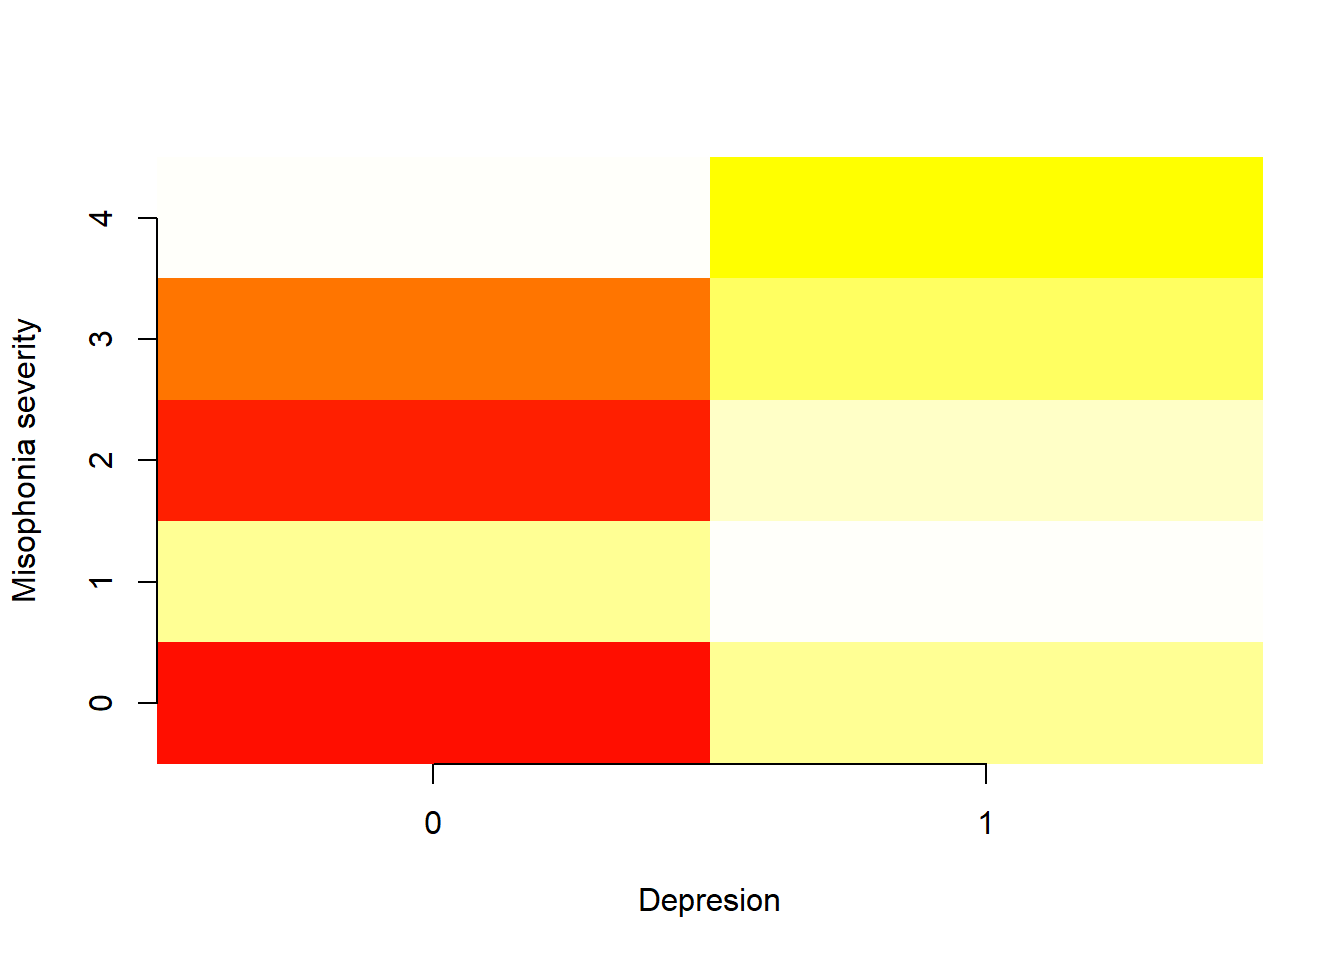
\includegraphics{_main_files/figure-latex/unnamed-chunk-30-1.pdf}

\begin{center}\rule{0.5\linewidth}{0.5pt}\end{center}

\begin{center}\rule{0.5\linewidth}{0.5pt}\end{center}

\hypertarget{variables-continuas-1}{%
\section{Variables continuas}\label{variables-continuas-1}}

En el estudio de misofonía también se midió la protrusión mandibular como posible factor cefalométrico de la enfermedad.

\begin{verbatim}
##     Angulo_convexidad protusion.mandibular
## 1                7.97                13.00
## 2               18.23                -5.00
## 3               12.27                11.50
## 4                7.81                16.80
## 5                9.81                33.00
## 6               13.50                 2.00
## 7               19.30                -3.90
## 8                7.70                16.80
## 9               12.30                 8.00
## 10               7.90                28.80
## 11              12.60                 3.00
## 12              19.00                -7.90
## 13               7.27                28.30
## 14              14.00                 4.00
## 15               5.40                22.20
## 16               8.00                 0.00
## 17              11.20                15.00
## 18               7.75                17.00
## 19               7.94                49.00
## 20              16.69                 5.00
## 21               7.62                42.00
## 22               7.02                28.00
## 23               7.00                 9.40
## 24              19.20               -13.20
## 25               7.96                23.00
## 26              14.70                 2.30
## 27               7.24                25.00
## 28               7.80                 4.90
## 29               7.90                92.00
## 30               4.70                 6.00
## 31               4.40                17.00
## 32              14.00                 3.30
## 33              14.40                10.30
## 34              16.00                 6.30
## 35               1.40                19.50
## 36               9.76                22.00
## 37               7.90                 5.00
## 38               7.90                78.00
## 39               7.40                 9.30
## 40               6.30                50.60
## 41               7.76                18.00
## 42               7.30                18.00
## 43               7.00                10.00
## 44              11.23                 4.00
## 45              16.00                13.30
## 46               7.90                48.00
## 47               7.29                23.50
## 48               6.91                37.60
## 49               7.10                15.00
## 50              13.40                 5.10
## 51              11.60                -2.20
## 52              -1.00                32.00
## 53               6.00                25.00
## 54               7.82                24.00
## 55               4.80                33.60
## 56              11.00                 3.30
## 57               9.00                31.50
## 58              11.50                12.80
## 59              16.00                 3.00
## 60              15.00                 6.00
## 61               1.40                21.40
## 62              16.80               -10.00
## 63               7.70                19.00
## 64              16.14                32.00
## 65               7.12                15.00
## 66              -1.00                10.00
## 67              17.00               -16.90
## 68               9.26                 2.00
## 69              18.70               -10.10
## 70               3.40                12.20
## 71              21.30               -11.00
## 72               7.50                 5.20
## 73               6.03                16.00
## 74               7.50                 5.80
## 75              19.00                 5.20
## 76              19.01                13.00
## 77               8.10                13.60
## 78               7.80                16.10
## 79               6.10                33.20
## 80              15.26                 4.00
## 81               7.95                12.00
## 82              18.00                -1.50
## 83               4.60                18.30
## 84              15.00                 3.00
## 85               7.50                15.80
## 86               8.00                27.10
## 87              16.80               -10.00
## 88               8.54                25.00
## 89               7.00                27.10
## 90              18.30                -8.00
## 91               7.80                12.00
## 92              16.00                -8.00
## 93              14.00                23.00
## 94              12.30                 5.00
## 95              11.40                 1.00
## 96               8.50                18.90
## 97               7.00                15.00
## 98               7.96                22.00
## 99              17.60                -3.50
## 100             10.00                20.00
## 101              3.50                12.20
## 102              6.70                14.70
## 103             17.00                -5.00
## 104             20.26                -4.15
## 105              6.64                11.00
## 106              1.80                -4.00
## 107              7.02                25.00
## 108              2.46                35.00
## 109             19.00                -5.00
## 110             17.86               -30.00
## 111              6.10                12.20
## 112              6.64                19.00
## 113             12.00                 1.60
## 114              6.60                20.00
## 115              8.70                17.10
## 116             14.05                24.00
## 117              7.20                 7.10
## 118             19.70               -11.00
## 119              7.70                21.30
## 120              6.02                 5.00
## 121              2.50                12.90
## 122             19.00                 5.90
## 123              6.80                 5.80
\end{verbatim}

\begin{center}\rule{0.5\linewidth}{0.5pt}\end{center}

\begin{center}\rule{0.5\linewidth}{0.5pt}\end{center}

\hypertarget{variables-continuas-2}{%
\section{Variables continuas}\label{variables-continuas-2}}

En el estudio de misofonía también se midió la protrusión mandibular como posible factor cefalométrico de la enfermedad.

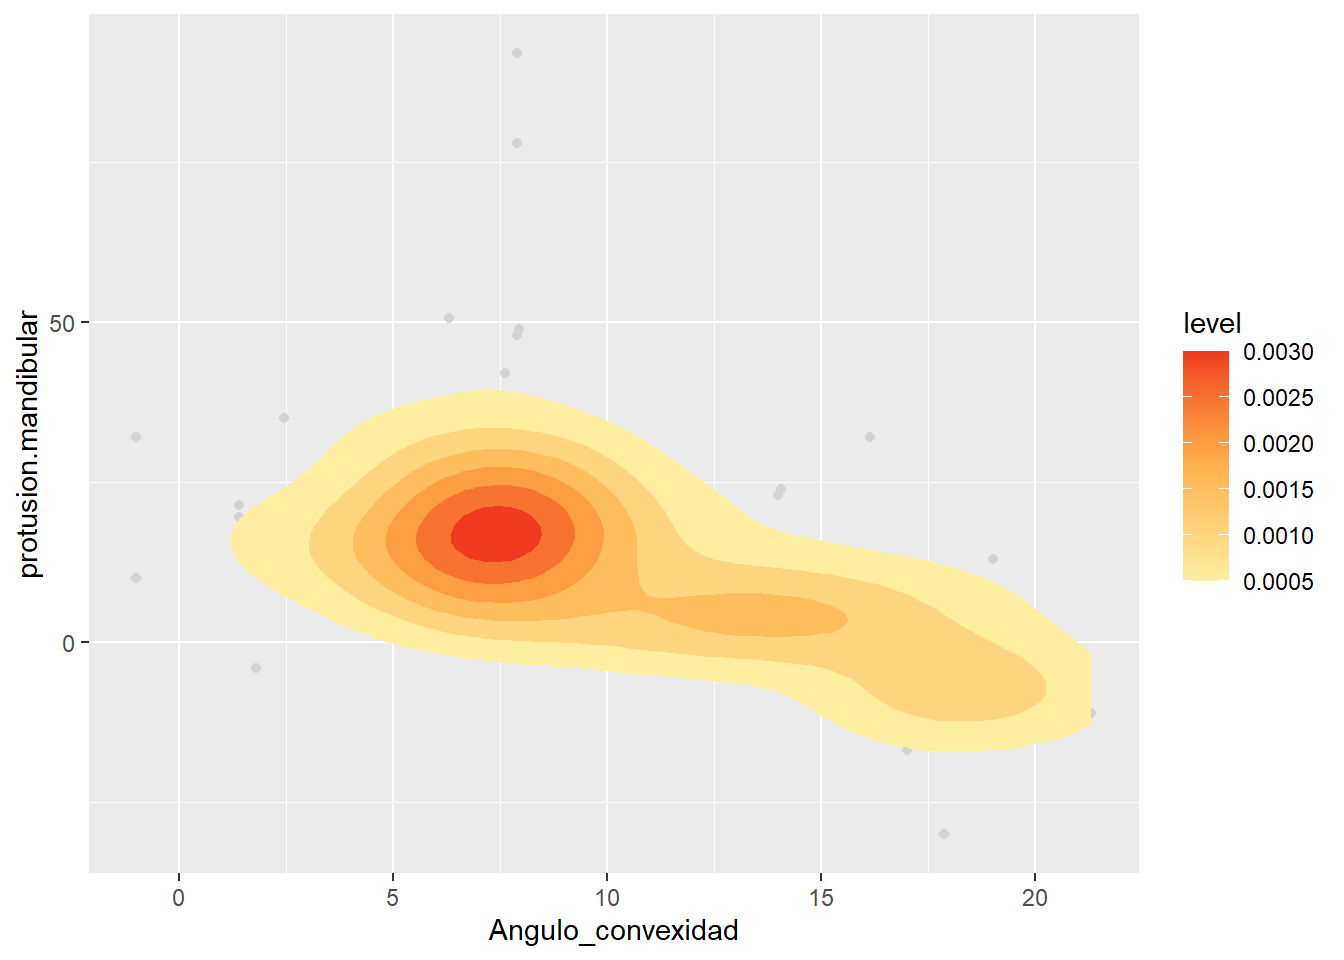
\includegraphics{_main_files/figure-latex/unnamed-chunk-32-1.pdf}

\begin{center}\rule{0.5\linewidth}{0.5pt}\end{center}

\begin{center}\rule{0.5\linewidth}{0.5pt}\end{center}

\hypertarget{gruxe1fico-de-dispersiuxf3n}{%
\section{Gráfico de dispersión}\label{gruxe1fico-de-dispersiuxf3n}}

\begin{itemize}
\item
  El \textbf{histograma} depende del tamaño del contenedor (píxel).
\item
  Si el píxel es lo suficientemente pequeño como para contener una sola observación, el mapa de calor da como resultado un \textbf{diagrama de dispersión}
\end{itemize}

El diagrama de dispersión es la ilustración de una ``tabla de contingencia'' para variables continuas cuando el contenedor (píxel) es lo suficientemente pequeño como para contener una sola observación (que consta de un par de valores).

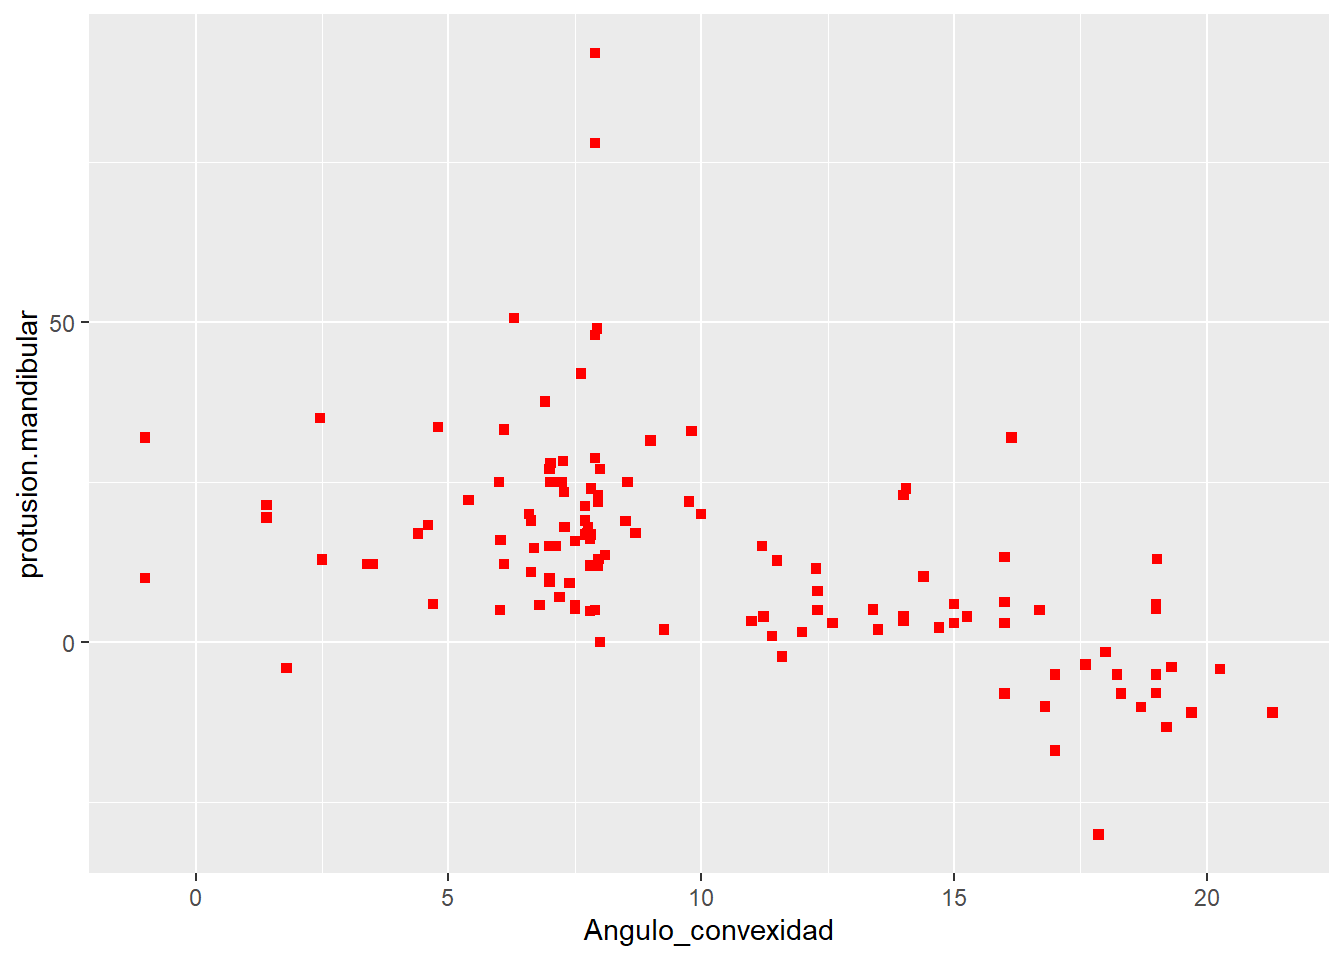
\includegraphics{_main_files/figure-latex/unnamed-chunk-33-1.pdf}

\hypertarget{probabilidad-condicional}{%
\chapter{Probabilidad condicional}\label{probabilidad-condicional}}

\hypertarget{objetivo-3}{%
\section{Objetivo}\label{objetivo-3}}

\begin{itemize}
\tightlist
\item
  Probabilidad condicional
\item
  Independencia
\item
  Teorema de Bayes
\end{itemize}

\begin{center}\rule{0.5\linewidth}{0.5pt}\end{center}

\begin{center}\rule{0.5\linewidth}{0.5pt}\end{center}

\hypertarget{probabilidad-conjunta}{%
\section{Probabilidad conjunta}\label{probabilidad-conjunta}}

La probabilidad conjunta de dos eventos \(A\) y \(B\) es
\[P(A,B)=P(A \cap B)\]

Imaginemos un experimento aleatorio que mide dos tipos diferentes de resultados.

\begin{itemize}
\item
  altura y peso de un individuo: \((h, w)\)
\item
  hora y lugar de una carga eléctrica: \((p, t)\)
\item
  una tirada de dos dados: (\(n_1\),\(n_2\))
\item
  cruzar dos semáforos en verde: (\(\bar{R_1}\), \(\bar{R_2}\))
\end{itemize}

En muchos casos, nos interesa saber si los valores de un resultado \textbf{condicionan} los valores del otro.

\begin{center}\rule{0.5\linewidth}{0.5pt}\end{center}

\begin{center}\rule{0.5\linewidth}{0.5pt}\end{center}

\hypertarget{diagnuxf3sticos}{%
\section{Diagnósticos}\label{diagnuxf3sticos}}

Consideremos una \textbf{herramienta de diagnóstico}

Queremos encontrar el estado de un sistema (s):

\begin{itemize}
\tightlist
\item
  inadecuado (sí)
\item
  adecuado (no)
\end{itemize}

con una prueba (t):

\begin{itemize}
\tightlist
\item
  positivo
\item
  negativo
\end{itemize}

Probamos una batería para saber cuánto tiempo puede vivir. Tensamos un cable para saber si resiste llevar cierta carga. Realizamos una PCR para ver si alguien está infectado.

\begin{center}\rule{0.5\linewidth}{0.5pt}\end{center}

\begin{center}\rule{0.5\linewidth}{0.5pt}\end{center}

\hypertarget{prueba-de-diagnuxf3stico}{%
\section{Prueba de diagnóstico}\label{prueba-de-diagnuxf3stico}}

Consideremos diagnosticar una infección con una nueva prueba.

Estado de infección:

\begin{itemize}
\tightlist
\item
  si (infectado)
\item
  no (no infectado)
\end{itemize}

Prueba:

\begin{itemize}
\tightlist
\item
  positivo
\item
  negativo
\end{itemize}

\begin{center}\rule{0.5\linewidth}{0.5pt}\end{center}

\begin{center}\rule{0.5\linewidth}{0.5pt}\end{center}

\hypertarget{observaciones}{%
\section{Observaciones}\label{observaciones}}

Cada individuo es un experimento aleatorio con dos medidas: (Infección, Prueba)

\begin{longtable}[]{@{}ccc@{}}
\toprule
Asunto & Infección & Prueba \\
\midrule
\endhead
\(s_1\) & si & positivo \\
\(s_2\) & no & negativo \\
\(s_3\) & si & positivo \\
\ldots{} & \ldots{} & \ldots{} \\
\(s_i\) & no & positivo* \\
\ldots{} & \ldots{} & \ldots{} \\
\ldots{} & \ldots{} & \ldots{} \\
\(s_n\) & si & negativo* \\
\bottomrule
\end{longtable}

\begin{center}\rule{0.5\linewidth}{0.5pt}\end{center}

\begin{center}\rule{0.5\linewidth}{0.5pt}\end{center}

\hypertarget{tablas-de-contingencia}{%
\section{Tablas de contingencia}\label{tablas-de-contingencia}}

\begin{itemize}
\tightlist
\item
  Por el número de observaciones de cada resultado
\end{itemize}

\begin{longtable}[]{@{}cccc@{}}
\toprule
& Infección: sí & Infección: no & suma \\
\midrule
\endhead
Test: positivo & 18 & 12 & 30 \\
Test: negativo & 30 & 300 & 330 \\
suma & 48 & 312 & 360 \\
\bottomrule
\end{longtable}

\begin{itemize}
\tightlist
\item
  Para las frecuencias relativas, si \(N>>0\) tomaremos \(f_{i,j}=\hat{P}(x_i, y_j)\)
\end{itemize}

\begin{longtable}[]{@{}cccc@{}}
\toprule
& Infección: sí & Infección: no & suma \\
\midrule
\endhead
Test: positivo & 0.05 & 0.0333 & 0.0833 \\
Test: negativo & 0.0833 & 0.833 & 0.9166 \\
suma & 0.133 & 0.866 & 1 \\
\bottomrule
\end{longtable}

\begin{center}\rule{0.5\linewidth}{0.5pt}\end{center}

\begin{center}\rule{0.5\linewidth}{0.5pt}\end{center}

\hypertarget{la-probabilidad-condicional}{%
\section{La probabilidad condicional}\label{la-probabilidad-condicional}}

Pensemos primero en términos de aquellos que están \textbf{infectados}

Dentro de los que están infectados (\textbf{sí}), ¿cuál es la probabilidad de dar positivo?

\begin{itemize}
\tightlist
\item
  Sensibilidad (tasa de verdaderos positivos)
\end{itemize}

\[\hat{P}(positivo|sí)=\frac{n_{positivo,sí}}{n_{sí}}\]

\[=\frac{\frac{n_{positivo,sí}}{N}}{\frac{n_{sí}}{N}}=\frac{f_{positivo,sí}}{f_{sí}} \]

Por lo tanto, en el límite, esperamos tener una probabilidad del tipo

\[P(positivo|sí)=\frac{P(positivo, sí)}{P(sí)}=\frac{P(positivo \cap sí)}{P(sí)}\]

\begin{center}\rule{0.5\linewidth}{0.5pt}\end{center}

\begin{center}\rule{0.5\linewidth}{0.5pt}\end{center}

\hypertarget{la-probabilidad-condicional-1}{%
\section{La probabilidad condicional}\label{la-probabilidad-condicional-1}}

\textbf{Definición:}
La probabilidad condicional de un evento B dado un evento A, denotado como \(P(A|B)\), es
\[P(A|B) = \frac{P(A\cap B)}{P(B)}\]

\begin{itemize}
\tightlist
\item
  se puede probar que la probabilidad condicional satisface los axiomas de probabilidad.
\item
  la probabilidad condicional es la probabilidad bajo el espacio muestral dado por \(B\): \(S_B\).
\end{itemize}

\begin{center}\rule{0.5\linewidth}{0.5pt}\end{center}

\begin{center}\rule{0.5\linewidth}{0.5pt}\end{center}

\hypertarget{tabla-de-contingencia-condicional}{%
\section{Tabla de contingencia condicional}\label{tabla-de-contingencia-condicional}}

\begin{longtable}[]{@{}ccc@{}}
\toprule
& Infección: Sí & Infección: No \\
\midrule
\endhead
Test: positivo & P(positivo {\textbar{}} sí) & P(positivo {\textbar{}} no) \\
Test: negativo & P(negativo {\textbar{}} sí) & P(negativo {\textbar{}} no) \\
suma & 1 & 1 \\
\bottomrule
\end{longtable}

\begin{itemize}
\item
  Tasa de verdaderos positivos (Sensibilidad): La probabilidad de dar positivo \textbf{si} se tiene la enfermedad \(P(positivo|sí)\)
\item
  Tasa de verdaderos negativos (Especificidad): La probabilidad de dar negativo \textbf{si} no se tiene la enfermedad \(P(negativo|no)\)
\item
  Tasa de falsos positivos: La probabilidad de dar positivo \textbf{si} no se tiene la enfermedad \(P(positivo|no)\)
\item
  Tasa de falsos negativos: la probabilidad de dar negativo \textbf{si} se tiene la enfermedad \(P(negativo|sí)\)
\end{itemize}

\begin{center}\rule{0.5\linewidth}{0.5pt}\end{center}

\begin{center}\rule{0.5\linewidth}{0.5pt}\end{center}

\hypertarget{ejemplo-de-tabla-de-contingencia-condicional}{%
\section{Ejemplo de tabla de contingencia condicional}\label{ejemplo-de-tabla-de-contingencia-condicional}}

Tomando las frecuencias como estimaciones de las probabilidades, entonces

\begin{longtable}[]{@{}ccc@{}}
\toprule
& Infección: Sí & Infección: No \\
\midrule
\endhead
Test: positivo & 18/48 = 0.375 & 12/312 = 0.038 \\
Test: negativo & 30/48 = 0.625 & 300/312 =0.962 \\
suma & 1 & 1 \\
\bottomrule
\end{longtable}

Nuestra herramienta de diagnóstico tiene baja sensibilidad (0.375) pero alta
especificidad (0.962).

\begin{center}\rule{0.5\linewidth}{0.5pt}\end{center}

\begin{center}\rule{0.5\linewidth}{0.5pt}\end{center}

\hypertarget{regla-de-multiplicaciuxf3n}{%
\section{Regla de multiplicación}\label{regla-de-multiplicaciuxf3n}}

Ahora imaginemos la situación real, donde queremos obtener la probabilidad \textbf{conjunta} de la probabilidad \textbf{condicional}

\begin{itemize}
\item
  Se (realizaron) PCR para coronavirus {[}\url{https://www.nejm.org/doi/full/10.1056/NEJMp2015897}{]} en personas en el hospital que estamos seguros de estar infectadas. Este test tiene una sensibilidad del 70\%. También se ha probado en el laboratorio en condiciones sin infección con una especificidad del 96 \%.
\item
  Un estudio de prevalencia en España mostró que \(P(sí)=0.05\), \(P(no)=0.95\) antes del verano.
\end{itemize}

Con estos datos, ¿cuál era la probabilidad de que una persona seleccionada al azar de la población diera positivo \textbf{y} estuviera infectada: \(P(sí \cap positivo)=P(sí, positivo)\)?

\begin{center}\rule{0.5\linewidth}{0.5pt}\end{center}

\begin{center}\rule{0.5\linewidth}{0.5pt}\end{center}

\hypertarget{rendimiento-de-diagnuxf3stico}{%
\section{Rendimiento de diagnóstico}\label{rendimiento-de-diagnuxf3stico}}

Para estudiar el rendimiento de una nueva prueba diagnóstica:

\begin{itemize}
\item
  selecciona muestras que son inadecuadas (enfermedad: \textbf{sí}) y aplica la prueba, tratando de encontrar su sensibilidad: \(P(positivo|sí)\) (\(0.70\) para PCR)
\item
  selecciona muestras que son adecuadas (enfermedad: \textbf{no}) y aplica la prueba, tratando de encontrar su especificidad: \(P(negativo|no)\) (\(0.96\) para PCR)
\end{itemize}

\begin{center}\rule{0.5\linewidth}{0.5pt}\end{center}

\begin{center}\rule{0.5\linewidth}{0.5pt}\end{center}

\begin{longtable}[]{@{}ccc@{}}
\toprule
& Infección: Sí & Infección: No \\
\midrule
\endhead
Test: positivo & P(positivo{\textbar{}}sí)=0.7 & P(positivo{\textbar{}}no)=0.06 \\
Test: negativo & P(negativo{\textbar{}}sí)=0.3 & P(negativo{\textbar{}}no)=0.94 \\
suma & 1 & 1 \\
\bottomrule
\end{longtable}

De esta matriz, ¿podemos obtener \(P(sí, positivo)\)?

\begin{center}\rule{0.5\linewidth}{0.5pt}\end{center}

\begin{center}\rule{0.5\linewidth}{0.5pt}\end{center}

\hypertarget{regla-de-multiplicaciuxf3n-1}{%
\section{Regla de multiplicación}\label{regla-de-multiplicaciuxf3n-1}}

¿Cómo se recupera la probabilidad conjunta de la probabilidad condicional?

Para dos eventos \(A\) y \(B\) tenemos la regla de la multiplicación

\[P(A, B) = P(A|B) P(B)\]

que se sigue de la definición de probabilidad condicional.

\begin{center}\rule{0.5\linewidth}{0.5pt}\end{center}

\begin{center}\rule{0.5\linewidth}{0.5pt}\end{center}

\hypertarget{tabla-de-contingencia-en-tuxe9rminos-de-probabilidades-condicionales}{%
\section{Tabla de contingencia en términos de probabilidades condicionales}\label{tabla-de-contingencia-en-tuxe9rminos-de-probabilidades-condicionales}}

\begin{longtable}[]{@{}cccc@{}}
\toprule
& Infección: Sí & Infección: No & suma \\
\midrule
\endhead
Test: positivo & P(positivo {\textbar{}} sí)P(sí) & P(positivo {\textbar{}} no)P(no) & P(positivo) \\
Test: negativo & P(negativo {\textbar{}} sí)P(sí) & P(negativo {\textbar{}} no) P(no) & P(negativo) \\
suma & P(sí) & P(no) & 1 \\
\bottomrule
\end{longtable}

Por ejemplo, la probabilidad de dar \(positivo\) y estar infectado \(sí\):

\begin{itemize}
\tightlist
\item
  \(P(positivo, sí)=P(positivo \cap sí) = P(positivo|sí) P(sí)\)
\end{itemize}

\begin{center}\rule{0.5\linewidth}{0.5pt}\end{center}

\begin{center}\rule{0.5\linewidth}{0.5pt}\end{center}

\hypertarget{uxe1rbol-condicional}{%
\section{Árbol condicional}\label{uxe1rbol-condicional}}

\begin{center}\rule{0.5\linewidth}{0.5pt}\end{center}

\begin{center}\rule{0.5\linewidth}{0.5pt}\end{center}

\hypertarget{tabla-de-contingencia-en-tuxe9rminos-de-probabilidades-condicionales-1}{%
\section{Tabla de contingencia en términos de probabilidades condicionales}\label{tabla-de-contingencia-en-tuxe9rminos-de-probabilidades-condicionales-1}}

\begin{longtable}[]{@{}cccc@{}}
\toprule
& Infección: sí & Infección: no & suma \\
\midrule
\endhead
Test: positivo & 0.035 & 0.057 & 0.092 \\
Test: negativo & 0.015 & 0.893 & 0.908 \\
suma & 0.05 & 0.95 & 1 \\
\bottomrule
\end{longtable}

\begin{itemize}
\tightlist
\item
  \(P(positivo,si)= 0.035\)
\end{itemize}

Pero también encontramos la probabilidad marginal de ser \textbf{positivo}:

\begin{itemize}
\tightlist
\item
  \(P(positivo)=0.092\)
\end{itemize}

\begin{center}\rule{0.5\linewidth}{0.5pt}\end{center}

\begin{center}\rule{0.5\linewidth}{0.5pt}\end{center}

\hypertarget{regla-de-probabilidad-total}{%
\section{Regla de probabilidad total}\label{regla-de-probabilidad-total}}

\begin{longtable}[]{@{}cccc@{}}
\toprule
& Infección: Sí & Infección: No & suma \\
\midrule
\endhead
Test: positivo & P(positivo {\textbar{}} sí)P(sí) & P(positivo {\textbar{}} no)P(no) & P(positivo) \\
Test: negativo & P(negativo {\textbar{}} sí)P(sí) & P(negativo {\textbar{}} no) P(no) & P(negativo) \\
suma & P(sí) & P(no) & 1 \\
\bottomrule
\end{longtable}

Cuando escribimos las marginales desconocidas en términos de sus probabilidades condicionales, lo llamamos \textbf{regla de probabilidad total}

\begin{itemize}
\tightlist
\item
  \(P(positivo)=P(positivo|sí)P(sí)+P(positivo|no)P(no)\)
\item
  \(P(negativo)=P(negativo|sí)P(sí)+P(negativo|no)P(no)\)
\end{itemize}

\begin{center}\rule{0.5\linewidth}{0.5pt}\end{center}

\begin{center}\rule{0.5\linewidth}{0.5pt}\end{center}

\hypertarget{uxe1rbol-condicional-1}{%
\section{Árbol condicional}\label{uxe1rbol-condicional-1}}

\textbf{Regla de probabilidad total} para la marginal de \(B\): ¿De cuántas maneras puedo obtener el resultado \(B\)?

\(P(B)=P(B|A)P(A)+P(B|A')P(A')\)

\begin{center}\rule{0.5\linewidth}{0.5pt}\end{center}

\begin{center}\rule{0.5\linewidth}{0.5pt}\end{center}

\hypertarget{encontrar-probabilidades-inversas}{%
\section{Encontrar probabilidades inversas}\label{encontrar-probabilidades-inversas}}

De la tabla de contingencia condicional

\begin{longtable}[]{@{}ccc@{}}
\toprule
& Infección: Sí & Infección: No \\
\midrule
\endhead
Test: positivo & P(positivo {\textbar{}} sí) & P(positivo {\textbar{}} no) \\
Test: negativo & P(negativo {\textbar{}} sí) & P(negativo {\textbar{}} no) \\
suma & 1 & 1 \\
\bottomrule
\end{longtable}

¿Cómo podemos calcular la probabilidad de estar infectado si la prueba da positivo: \(P(sí|positivo)\)?

\begin{center}\rule{0.5\linewidth}{0.5pt}\end{center}

\begin{center}\rule{0.5\linewidth}{0.5pt}\end{center}

\hypertarget{recuperar-probabilidades-conjuntas}{%
\section{Recuperar probabilidades conjuntas}\label{recuperar-probabilidades-conjuntas}}

\begin{enumerate}
\def\labelenumi{\arabic{enumi}.}
\tightlist
\item
  Recuperamos la tabla de contingencia para probabilidades conjuntas
\end{enumerate}

\begin{longtable}[]{@{}cccc@{}}
\toprule
& Infección: Sí & Infección: No & suma \\
\midrule
\endhead
Test: positivo & P(positivo {\textbar{}} sí)P(sí) & P(positivo {\textbar{}} no)P(no) & P(positivo) \\
Test: negativo & P(negativo {\textbar{}} sí)P(sí) & P(negativo {\textbar{}} no) P(no) & P(negativo) \\
suma & P(sí) & P(no) & 1 \\
\bottomrule
\end{longtable}

\begin{center}\rule{0.5\linewidth}{0.5pt}\end{center}

\begin{center}\rule{0.5\linewidth}{0.5pt}\end{center}

\hypertarget{condicionales-inversas}{%
\section{Condicionales inversas}\label{condicionales-inversas}}

\begin{enumerate}
\def\labelenumi{\arabic{enumi}.}
\setcounter{enumi}{1}
\tightlist
\item
  Calculamos las probabilidades condicionales para la prueba:
\end{enumerate}

\[P(infección|prueba)=\frac{P(prueba|infección)P(infección)}{P(prueba)}\]

\begin{longtable}[]{@{}cccc@{}}
\toprule
& Infección: Sí & Infección: No & suma \\
\midrule
\endhead
Test: positivo & P(sí{\textbar{}}positivo) & P(sin{\textbar{}}positivo) & 1 \\
Test: negativo & P(sí{\textbar{}}negativo) & P(sin{\textbar{}}negativo) & 1 \\
\bottomrule
\end{longtable}

Por ejemplo:
\[P(sí|positivo)=\frac{P(positivo|sí)P(sí)}{P(positivo)}\]
como normalmente no tenemos \(P(positivo)\), usamos la regla de \textbf{probabilidad total} en el denominador

\[P(sí|positivo)=\frac{P(positivo|sí)P(sí)}{P(positivo|sí)P(sí)+P(positivo|no)P(no)}\]

\begin{center}\rule{0.5\linewidth}{0.5pt}\end{center}

\begin{center}\rule{0.5\linewidth}{0.5pt}\end{center}

\hypertarget{teorema-de-bayes}{%
\section{Teorema de Bayes}\label{teorema-de-bayes}}

La expresion:

\[P(sí|positivo)=\frac{P(positivo|sí)P(sí)}{P(positivo|sí)P(sí)+P(positivo|no)P(no)}\]

se llama \textbf{teorema de Bayes}

\textbf{Teorema}

Si \(E1, E2, ..., Ek\) son \(k\) eventos mutuamente excluyentes y exhaustivos y \(B\) es cualquier evento,

\[P(Ei|B)=\frac{P(B|Ei)P(Ei)}{P(B|E1)P(E1) +...+ P(B|Ek)P(Ek)} \]

Permite invertir los condicionales:

\[P(B|A) \rightarrow P(A|B)\]

O \textbf{diseñe} una prueba \(B\) en condición controlada \(A\) y luego utilícela para \textbf{inferir} la probabilidad de la condición cuando la prueba es positiva.

\begin{center}\rule{0.5\linewidth}{0.5pt}\end{center}

\begin{center}\rule{0.5\linewidth}{0.5pt}\end{center}

\hypertarget{ejemplo-teorema-de-bayes}{%
\section{Ejemplo: teorema de Bayes}\label{ejemplo-teorema-de-bayes}}

Teorema de Bayes:

\[P(sí|positivo) = \frac{P(positivo|sí) P(sí)}{P(positivo|sí)P(sí)+P(positivo|no)P(no)}\]

sabemos:

\begin{itemize}
\item
  \(P(positivo|sí)=0.70\)
\item
  \(P(positivo|no)=1- P(negativo|no)=0.06\)
\item
  la probabilidad de infección y no infección en la población: \(P(sí)=0.05\) y \(P(no)=1-P(sí)=0.95\).
\end{itemize}

Por lo tanto:

\[P(sí|positivo)=0.47\]

Las pruebas no son tan buenas para \textbf{confirmar} infecciones.

\begin{center}\rule{0.5\linewidth}{0.5pt}\end{center}

\begin{center}\rule{0.5\linewidth}{0.5pt}\end{center}

\hypertarget{ejemplo-teorema-de-bayes-1}{%
\section{Ejemplo: teorema de Bayes}\label{ejemplo-teorema-de-bayes-1}}

Apliquémoslo ahora a la probabilidad de no estar infectado si la prueba es negativa.

\[P(no|negativo) = \frac{P(negativo|no) P(no)}{P(negativo|no) P(no)+P(negativo|sí)P(sí)}\]

La sustitución de todos los valores da

\[P(no|negativo)=0.98\]

Las pruebas son buenas para \textbf{descartar} infecciones.

\begin{center}\rule{0.5\linewidth}{0.5pt}\end{center}

\begin{center}\rule{0.5\linewidth}{0.5pt}\end{center}

\hypertarget{independencia-estaduxedstica}{%
\section{Independencia estadística}\label{independencia-estaduxedstica}}

En muchas aplicaciones, queremos saber si el conocimiento de un evento condiciona el resultado de otro evento.

\begin{itemize}
\tightlist
\item
  hay casos en los que queremos saber si los eventos no están condicionados
\end{itemize}

\begin{center}\rule{0.5\linewidth}{0.5pt}\end{center}

\begin{center}\rule{0.5\linewidth}{0.5pt}\end{center}

\hypertarget{independencia-estaduxedstica-1}{%
\section{Independencia estadística}\label{independencia-estaduxedstica-1}}

Considere los conductores para los cuales medimos sus fallas superficiales y si su capacidad de conducción es defectuosa.

Las \textbf{probabilidades conjuntas} estimadas son

\begin{longtable}[]{@{}cccc@{}}
\toprule
& fallas (F) & sin fallas (F') & suma \\
\midrule
\endhead
defectuoso (D) & \(0.005\) & \(0.045\) & \(0.05\) \\
sin defectos (D') & \(0.095\) & \(0.855\) & \(0.95\) \\
suma & \(0.1\) & \(0.9\) & 1 \\
\bottomrule
\end{longtable}

donde, por ejemplo, la probabilidad conjunta de \(F\) y \(D\) es

\begin{itemize}
\tightlist
\item
  \(P(D,F)=0.005\)
\end{itemize}

Las probabilidades marginales son

\begin{itemize}
\tightlist
\item
  \(P(D)=P(D, F) + P(D, F')=0.05\)
\item
  \(P(F)=P(D, F) + P(D', F)= 0.1\).
\end{itemize}

\begin{center}\rule{0.5\linewidth}{0.5pt}\end{center}

\begin{center}\rule{0.5\linewidth}{0.5pt}\end{center}

\hypertarget{independencia-estaduxedstica-2}{%
\section{Independencia estadística}\label{independencia-estaduxedstica-2}}

¿Cuál es la \textbf{probabilidad condicional} de observar un conductor defectuoso si tiene un defecto?

\begin{longtable}[]{@{}ccc@{}}
\toprule
& F & F' \\
\midrule
\endhead
D & P(D{\textbar{}}F) = 0.05 & P(D{\textbar{}}F')=0.05 \\
D' & P(D'{\textbar{}}F)=0.95 & P(D'{\textbar{}}F')=0.95 \\
suma & 1 & 1 \\
\bottomrule
\end{longtable}

¡Las probabilidades marginales y condicionales son las mismas!

\begin{itemize}
\tightlist
\item
  \(P(D|F)=P(D|F')=P(D)\)
\item
  \(P(D'|F)=P(D'|F')=P(D')\)
\end{itemize}

La probabilidad de observar un conductor defectuoso \textbf{no} depende de haber observado o no un defecto.

\[P(D) = P(D|F)\]

\begin{center}\rule{0.5\linewidth}{0.5pt}\end{center}

\begin{center}\rule{0.5\linewidth}{0.5pt}\end{center}

\hypertarget{independencia-estaduxedstica-3}{%
\section{Independencia estadística}\label{independencia-estaduxedstica-3}}

Dos eventos \(A\) y \(B\) son estadísticamente independientes si

\begin{itemize}
\tightlist
\item
  \(P(A|B)=P(A)\); \(A\) es independiente de \(B\)
\item
  \(P(B|A)=P(B)\); \(B\) es independiente de \(A\)
\end{itemize}

y por la regla de la multiplicación, su probabilidad conjunta es

\begin{itemize}
\tightlist
\item
  \(P(A\cap B)=P(A|B)P(B)=P(A)P(B)\)
\end{itemize}

la multiplicación de sus probabilidades marginales.

\begin{center}\rule{0.5\linewidth}{0.5pt}\end{center}

\begin{center}\rule{0.5\linewidth}{0.5pt}\end{center}

\hypertarget{productos-de-productos-marginales}{%
\section{Productos de productos marginales}\label{productos-de-productos-marginales}}

\begin{longtable}[]{@{}cccc@{}}
\toprule
& F & F' & suma \\
\midrule
\endhead
D & \(0.005\) & \(0.045\) & \(0.05\) \\
D' & \(0.095\) & \(0.855\) & \(0.95\) \\
suma & \(0.1\) & \(0.9\) & 1 \\
\bottomrule
\end{longtable}

Confirme que todas las entradas de la matriz son el producto de los marginales.

Por ejemplo:

\begin{itemize}
\tightlist
\item
  \(P(F)P(D)= P(D \cap F)\)
\item
  \(P(D')P(F')=P(D' \cap F')\)
\end{itemize}

\begin{center}\rule{0.5\linewidth}{0.5pt}\end{center}

\begin{center}\rule{0.5\linewidth}{0.5pt}\end{center}

\hypertarget{ejemplo-5}{%
\section{Ejemplo}\label{ejemplo-5}}

Resultados de lanzar dos monedas: \(S={(H,H), (H,T), (T,H), (T,T)}\)

\begin{longtable}[]{@{}cccc@{}}
\toprule
& H & T & suma \\
\midrule
\endhead
H & \(1/4\) & \(1/4\) & \(1/2\) \\
T & \(1/4\) & \(1/4\) & \(1/2\) \\
suma & \(1/2\) & \(1/2\) & 1 \\
\bottomrule
\end{longtable}

\begin{itemize}
\tightlist
\item
  Obtener cara en la primera moneda no condiciona obtener cruz en el resultado de la segunda moneda \(P(T|H)=P(T)=1/2\)
\item
  la probabilidad de obtener cara y después cruz es el producto de cada resultado independiente \(P(H, T)=P(H)*P(T)=1/4\)
\end{itemize}

\begin{center}\rule{0.5\linewidth}{0.5pt}\end{center}

\begin{center}\rule{0.5\linewidth}{0.5pt}\end{center}

\hypertarget{variables-aleatorias-discretas}{%
\chapter{Variables aleatorias discretas}\label{variables-aleatorias-discretas}}

\hypertarget{objetivo-4}{%
\section{Objetivo}\label{objetivo-4}}

\begin{itemize}
\tightlist
\item
  Variables aleatorias
\item
  Función de probabilidad
\item
  Media y varianza
\item
  Distribución de probabilidad
\end{itemize}

\begin{center}\rule{0.5\linewidth}{0.5pt}\end{center}

\begin{center}\rule{0.5\linewidth}{0.5pt}\end{center}

\hypertarget{cuxf3mo-asignamos-valores-de-probabilidad-a-los-resultados}{%
\section{¿Cómo asignamos valores de probabilidad a los resultados?}\label{cuxf3mo-asignamos-valores-de-probabilidad-a-los-resultados}}

\begin{center}\rule{0.5\linewidth}{0.5pt}\end{center}

\begin{center}\rule{0.5\linewidth}{0.5pt}\end{center}

\hypertarget{variable-aleatoria}{%
\section{Variable aleatoria}\label{variable-aleatoria}}

\textbf{Definición:}

Una \textbf{variable aleatoria} es una función que asigna un \textbf{número} real a cada \textbf{resultado} en el espacio muestral de un experimento aleatorio.

\begin{itemize}
\tightlist
\item
  Por lo general, una variable aleatoria es el valor de la \textbf{medida} de interés que se realiza en un experimento aleatorio.
\end{itemize}

Una variable aleatoria puede ser:

\begin{itemize}
\tightlist
\item
  Discreta (nominal, ordinal)
\item
  Continua (intervalo, relación)
\end{itemize}

\begin{center}\rule{0.5\linewidth}{0.5pt}\end{center}

\begin{center}\rule{0.5\linewidth}{0.5pt}\end{center}

\hypertarget{variable-aleatoria-1}{%
\section{Variable aleatoria}\label{variable-aleatoria-1}}

Un \textbf{valor} (o \textbf{resultado}) de una variable aleatoria es uno de los números posibles que la variable puede tomar en un experimento aleatorio.

Escribimos la variable aleatoria en \textbf{mayúsculas}.

Ejemplo:

Si \(X \in \{0,1\}\), entonces decimos que \(X\) es una variable aleatoria que puede tomar los valores \(0\) o \(1\).

\textbf{Observación} de una variable aleatoria

\begin{itemize}
\tightlist
\item
  Una observación es la \textbf{adquisición} del valor de una variable aleatoria en un experimento aleatorio
\end{itemize}

Ejemplo:

1 0 0 1 0 \textbf{1} 0 1 1

El número en negrita es una observación de \(X\)

\begin{center}\rule{0.5\linewidth}{0.5pt}\end{center}

\begin{center}\rule{0.5\linewidth}{0.5pt}\end{center}

\hypertarget{eventos-de-observar-una-variable-aleatoria}{%
\section{Eventos de observar una variable aleatoria}\label{eventos-de-observar-una-variable-aleatoria}}

\begin{itemize}
\tightlist
\item
  \(X=1\) es el \textbf{evento} de observar la variable aleatoria \(X\) con valor \(1\)
\item
  \(X=2\) es el \textbf{evento} de observar la variable aleatoria \(X\) con valor \(2\)
\end{itemize}

\ldots{}

\textbf{En general:}

\begin{itemize}
\item
  \(X=x\) es el \textbf{evento} de observar la variable aleatoria \(X\) con valor \(x\) (pequeño \(x\))
\item
  Dos valores cualesquiera de una variable aleatoria definen dos eventos \textbf{mutuamente excluyentes}.
\end{itemize}

\begin{center}\rule{0.5\linewidth}{0.5pt}\end{center}

\begin{center}\rule{0.5\linewidth}{0.5pt}\end{center}

\hypertarget{probabilidad-de-variables-aleatorias}{%
\section{Probabilidad de variables aleatorias}\label{probabilidad-de-variables-aleatorias}}

Nos interesa asignar probabilidades a los valores de una variable aleatoria.

Ya hemos hecho esto para los dados: \(X \in \{1,2,3,4,5,6\}\) (interpretación clásica de probabilidad)

\begin{longtable}[]{@{}cc@{}}
\toprule
\(X\) & Probabilidad \\
\midrule
\endhead
\(1\) & \(P(X=1)=1/6\) \\
\(2\) & \(P(X=2)=1/6\) \\
\(3\) & \(P(X=3)=1/6\) \\
\(4\) & \(P(X=4)=1/6\) \\
\(5\) & \(P(X=5)=1/6\) \\
\(6\) & \(P(X=6)=1/6\) \\
\bottomrule
\end{longtable}

\begin{center}\rule{0.5\linewidth}{0.5pt}\end{center}

\begin{center}\rule{0.5\linewidth}{0.5pt}\end{center}

\hypertarget{funciones-de-probabilidad}{%
\section{Funciones de probabilidad}\label{funciones-de-probabilidad}}

\begin{itemize}
\tightlist
\item
  Podemos escribir la tabla de probabilidad
\item
  graficarla
\end{itemize}

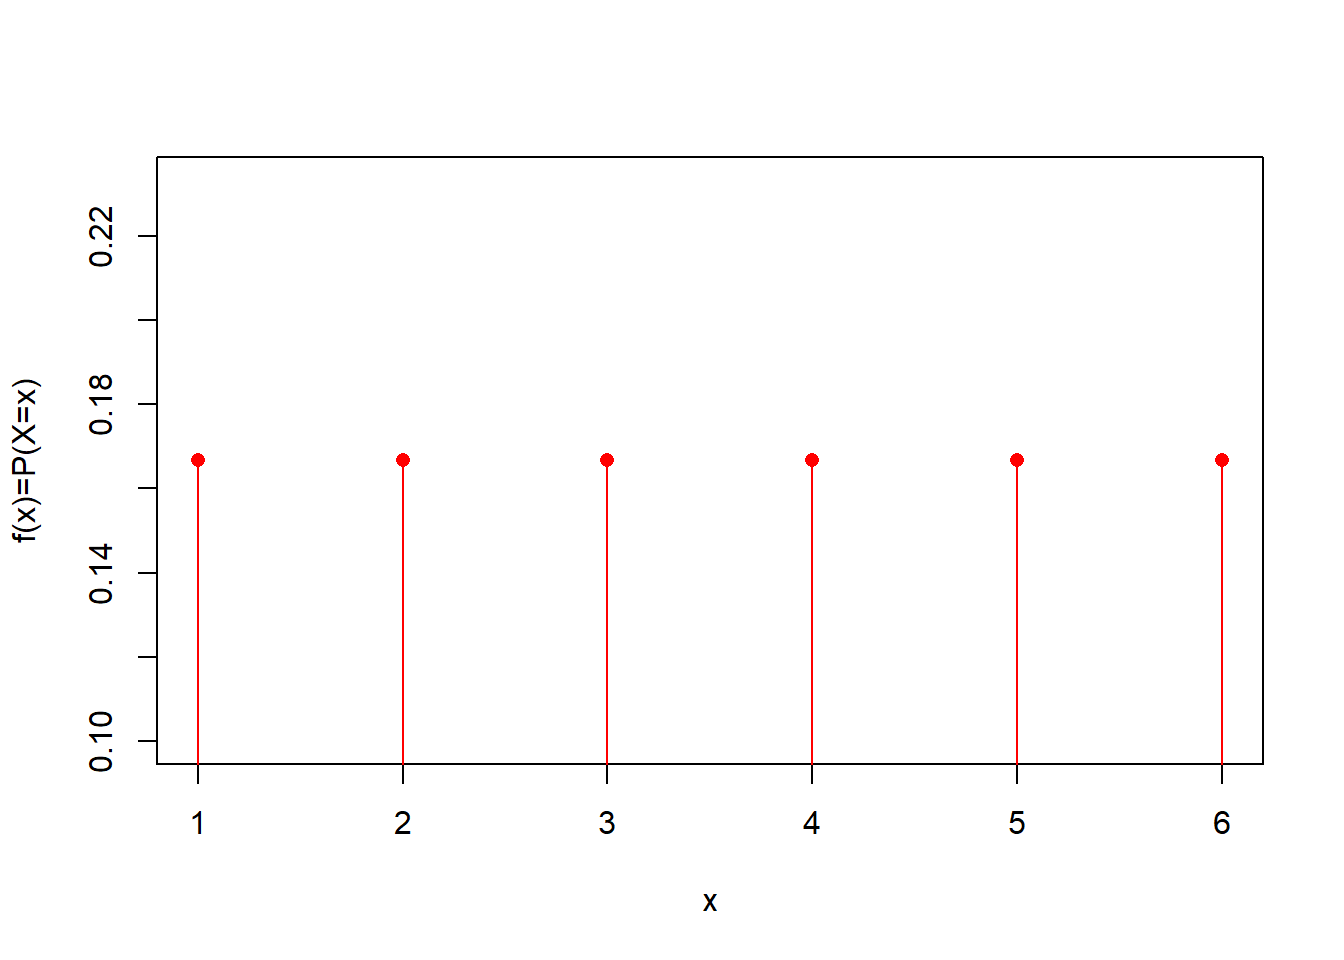
\includegraphics{_main_files/figure-latex/unnamed-chunk-34-1.pdf}

\begin{itemize}
\tightlist
\item
  o escribirla como la función
\end{itemize}

\[f(x)=P(X=x)=1/6\]

\begin{center}\rule{0.5\linewidth}{0.5pt}\end{center}

\begin{center}\rule{0.5\linewidth}{0.5pt}\end{center}

\hypertarget{funciones-de-probabilidad-1}{%
\section{Funciones de probabilidad}\label{funciones-de-probabilidad-1}}

Podemos \textbf{crear} cualquier tipo de función de probabilidad si respetamos las reglas de probabilidad:

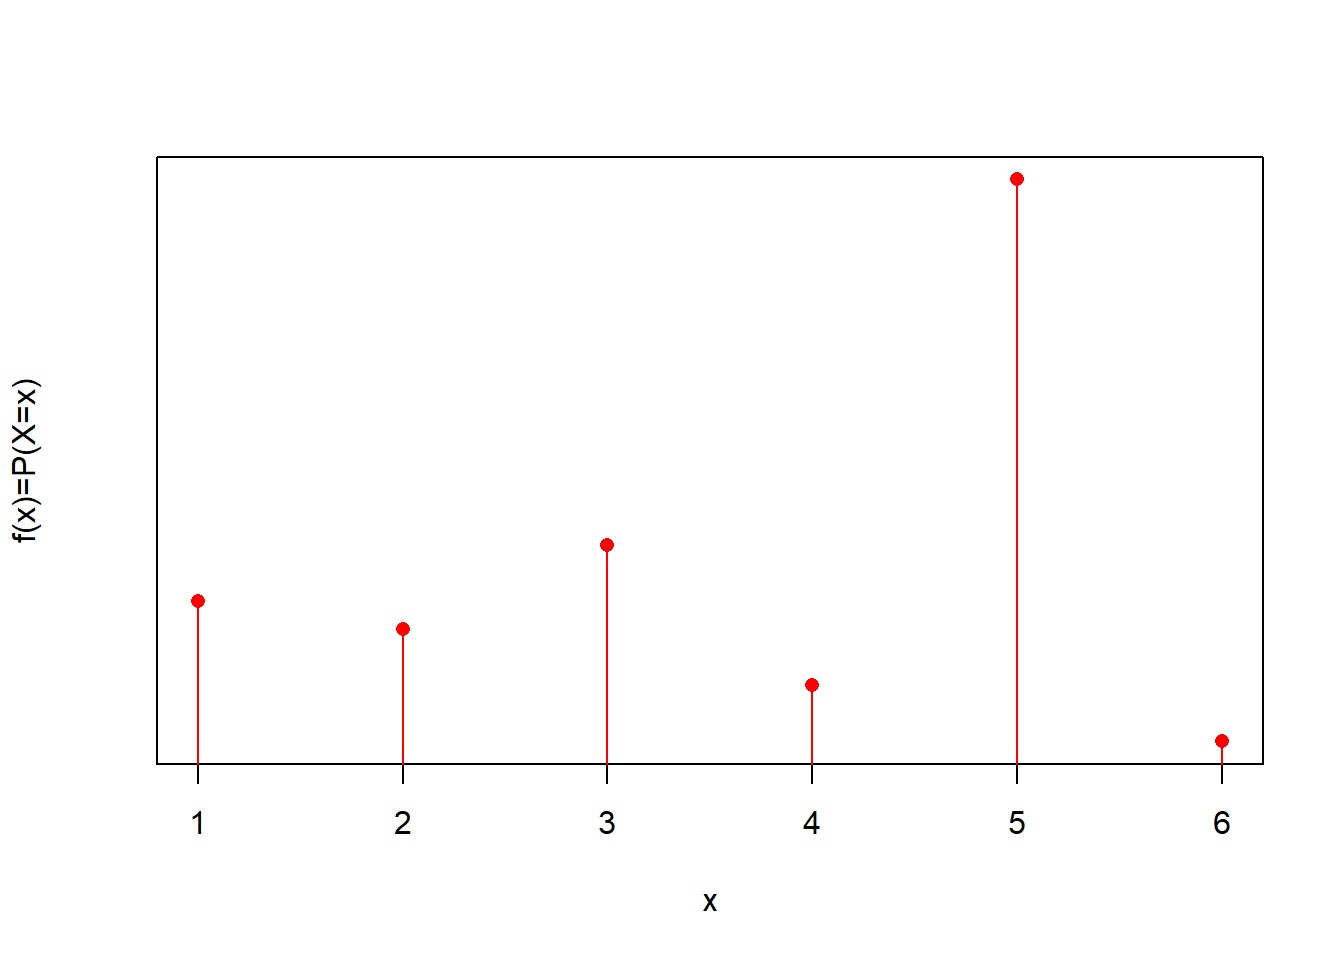
\includegraphics{_main_files/figure-latex/unnamed-chunk-35-1.pdf}

\begin{center}\rule{0.5\linewidth}{0.5pt}\end{center}

\begin{center}\rule{0.5\linewidth}{0.5pt}\end{center}

\hypertarget{funciones-de-probabilidad-2}{%
\section{Funciones de probabilidad}\label{funciones-de-probabilidad-2}}

Para una variable aleatoria discreta \(X \in \{x_1 , x_2 , .. , x_M\}\) , una \textbf{función de masa de probabilidad}

siempre es positiva

\begin{itemize}
\tightlist
\item
  \(f(x_i)\geq 0\)
\end{itemize}

se utiliza para calcular probabilidades

\begin{itemize}
\tightlist
\item
  \(f(x_i)=P(X=x_i)\)
\end{itemize}

y su suma sobre todos los valores de la variable es \(1\):

\begin{itemize}
\tightlist
\item
  \(\sum_{i=1}^M f(x_i)=1\)
\end{itemize}

\begin{center}\rule{0.5\linewidth}{0.5pt}\end{center}

\begin{center}\rule{0.5\linewidth}{0.5pt}\end{center}

\hypertarget{funciones-de-probabilidad-3}{%
\section{Funciones de probabilidad}\label{funciones-de-probabilidad-3}}

\begin{itemize}
\item
  Tenga en cuenta que la definición de \(X\) y su función de masa de probabilidad es general \textbf{sin referencia} a ningún experimento. Las funciones viven en el espacio modelo (abstracto).
\item
  \(X\) y \(f(x)\) son objetos abstractos que pueden o no asignarse a un experimento
\item
  Tenemos la libertad de construirlos como queramos siempre que respetemos su definición.
\item
  Tienen algunas \textbf{propiedades} que se derivan exclusivamente de su definición.
\end{itemize}

\begin{center}\rule{0.5\linewidth}{0.5pt}\end{center}

\begin{center}\rule{0.5\linewidth}{0.5pt}\end{center}

\hypertarget{ejemplo-funciuxf3n-de-masa-de-probabilidad}{%
\section{Ejemplo: función de masa de probabilidad}\label{ejemplo-funciuxf3n-de-masa-de-probabilidad}}

Considere la siguiente variable aleatoria \(X\) sobre los resultados

\begin{longtable}[]{@{}cc@{}}
\toprule
resultado & \(X\) \\
\midrule
\endhead
\(a\) & 0 \\
\(b\) & 0 \\
\(c\) & 1.5 \\
\(d\) & 1.5 \\
\(e\) & 2 \\
\(f\) & 3 \\
\bottomrule
\end{longtable}

Si cada resultado es igualmente probable, ¿cuál es la función de masa de probabilidad de \(x\)?

\begin{center}\rule{0.5\linewidth}{0.5pt}\end{center}

\begin{center}\rule{0.5\linewidth}{0.5pt}\end{center}

\hypertarget{tabla-de-probabilidad-para-resultados-igualmente-probables}{%
\section{Tabla de probabilidad para resultados igualmente probables}\label{tabla-de-probabilidad-para-resultados-igualmente-probables}}

\begin{longtable}[]{@{}cc@{}}
\toprule
resultado & Probabilidad (resultado) \\
\midrule
\endhead
\(a\) & \(1/6\) \\
\(b\) & \(1/6\) \\
\(c\) & \(1/6\) \\
\(d\) & \(1/6\) \\
\(e\) & \(1/6\) \\
\(f\) & \(1/6\) \\
\bottomrule
\end{longtable}

\begin{center}\rule{0.5\linewidth}{0.5pt}\end{center}

\begin{center}\rule{0.5\linewidth}{0.5pt}\end{center}

\hypertarget{tabla-de-probabilidad-para-x}{%
\section{\texorpdfstring{Tabla de probabilidad para \(X\)}{Tabla de probabilidad para X}}\label{tabla-de-probabilidad-para-x}}

\begin{longtable}[]{@{}cc@{}}
\toprule
\(X\) & \(f(x)=P(X=x)\) \\
\midrule
\endhead
\(0\) & \(P(X=0)=2/6\) \\
\(1.5\) & \(P(X=1.5)=2/6\) \\
\(2\) & \(P(X=2)=1/6\) \\
\(3\) & \(P(X=3)=1/6\) \\
\bottomrule
\end{longtable}

Podemos calcular, por ejemplo, las siguientes probabilidades de eventos en los valores de \(X\)

\begin{itemize}
\tightlist
\item
  \(P(X>3)\)
\item
  \(P(X=0\, \cup\, X=2 )\)
\item
  \(P(X \leq 2)\)
\end{itemize}

\begin{center}\rule{0.5\linewidth}{0.5pt}\end{center}

\begin{center}\rule{0.5\linewidth}{0.5pt}\end{center}

\hypertarget{ejemplo-6}{%
\section{Ejemplo}\label{ejemplo-6}}

\textbf{Modelo de probabilidad:}

Considere el siguiente experimento: En una urna ponga \(8\) bolas y:

\begin{itemize}
\tightlist
\item
  marque \(1\) bola con el número \(-2\)
\item
  marque \(2\) bolas con el número \(-1\)
\item
  marque \(2\) bolas con el número \(0\)
\item
  marque \(2\) bolas con el número \(1\)
\item
  marque \(1\) bola con el número \(2\)
\end{itemize}

\textbf{experimento:} Tome una bola y lea el número.

\begin{longtable}[]{@{}cc@{}}
\toprule
\(X\) & \(P(X=x)\) \\
\midrule
\endhead
\(-2\) & \(1/8=0.125\) \\
\(-1\) & \(2/8=0.25\) \\
\(0\) & \(2/8=0.25\) \\
\(1\) & \(2/8=0.25\) \\
\(2\) & \(1/8=0.125\) \\
\bottomrule
\end{longtable}

\begin{center}\rule{0.5\linewidth}{0.5pt}\end{center}

\begin{center}\rule{0.5\linewidth}{0.5pt}\end{center}

\hypertarget{ejemplo-7}{%
\section{Ejemplo}\label{ejemplo-7}}

Considere otro experimento en el que no sabemos qué hay en la urna anterior. Sacamos una bola \(30\) veces, escribimos su númeror y la devolvemos a la urna.

\begin{itemize}
\item
  no sabemos cuáles son los eventos primarios con iguales probabilidades.
\item
  y \textbf{estimamos} la \textbf{función de masa de probabilidad} a partir de las \textbf{frecuencias relativas} observadas para cada variable aleatoria
\end{itemize}

\begin{longtable}[]{@{}cc@{}}
\toprule
\(X\) & \(f_i\) \\
\midrule
\endhead
\(-2\) & \(0.132\) \\
\(-1\) & \(0.262\) \\
\(0\) & \(0.240\) \\
\(1\) & \(0.248\) \\
\(2\) & \(0.118\) \\
\bottomrule
\end{longtable}

\begin{center}\rule{0.5\linewidth}{0.5pt}\end{center}

\begin{center}\rule{0.5\linewidth}{0.5pt}\end{center}

\hypertarget{probabilidades-y-frecuencias}{%
\section{Probabilidades y frecuencias}\label{probabilidades-y-frecuencias}}

Para calcular las frecuencias relativas \(f_i\) trenemos que

\begin{itemize}
\tightlist
\item
  \textbf{repetir} el experimento \(N\) veces (tenemos que volver a poner la bola en la urna cada vez) y al final calcular
\end{itemize}

\[f_i=n_i/N\]

Estamos suponiendo que:

\[lim_{N \rightarrow \infty} f_i = f(x_i)=P(X=x_i)\]

\begin{center}\rule{0.5\linewidth}{0.5pt}\end{center}

\begin{center}\rule{0.5\linewidth}{0.5pt}\end{center}

\hypertarget{probabilidades-y-frecuencias-relativas}{%
\section{Probabilidades y frecuencias relativas}\label{probabilidades-y-frecuencias-relativas}}

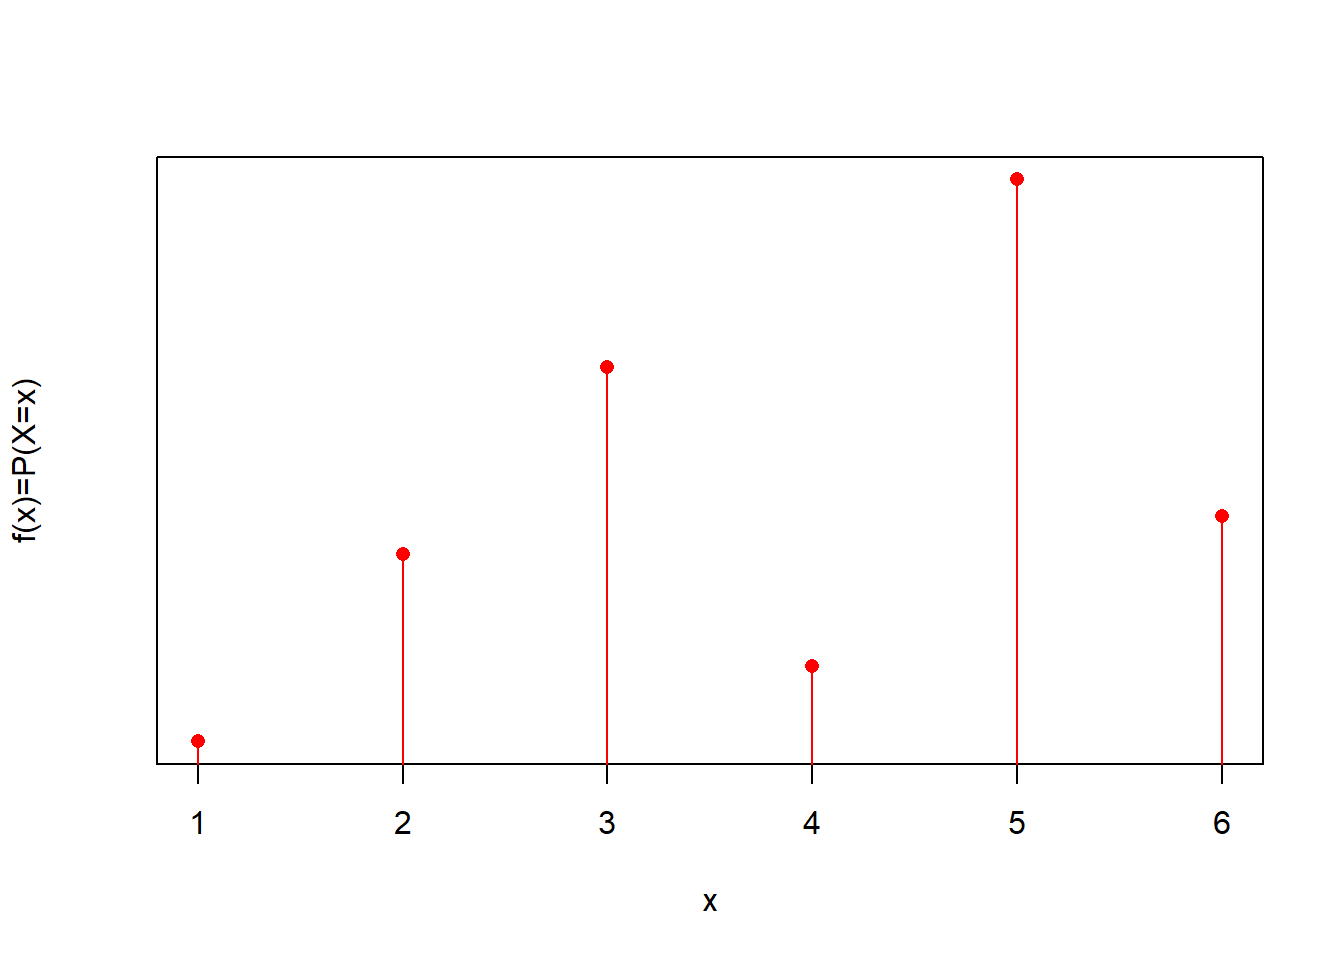
\includegraphics{_main_files/figure-latex/unnamed-chunk-36-1.pdf}

\begin{itemize}
\tightlist
\item
  En este ejemplo, \textbf{sabemos} el \textbf{modelo} de probabilidad \(f(x)=P(X=x)\) por diseño.
\item
  Nunca observamos \(f(x)\)
\item
  Podemos usar frecuencias relativas para estimar las probabilidades
  \[f_i = \hat{f}(x_i)=\hat{P}(X=x_i)\] (\(f_i\) depende de \(N\))
\end{itemize}

\begin{center}\rule{0.5\linewidth}{0.5pt}\end{center}

\begin{center}\rule{0.5\linewidth}{0.5pt}\end{center}

\hypertarget{media-y-varianza}{%
\section{Media y Varianza}\label{media-y-varianza}}

Las funciones de masa de probabilidad \(f(x)\) tienen dos propiedades principales

\begin{itemize}
\tightlist
\item
  su centro
\item
  su dispersión
\end{itemize}

Podemos preguntar,

\begin{itemize}
\item
  ¿Alrededor de qué valores de \(X\) se concentró la probabilidad?
\item
  ¿Qué tan dispersos son los valores de \(X\) en relación a sus probabilidades?
\end{itemize}

\begin{center}\rule{0.5\linewidth}{0.5pt}\end{center}

\begin{center}\rule{0.5\linewidth}{0.5pt}\end{center}

\hypertarget{media-y-varianza-1}{%
\section{Media y Varianza}\label{media-y-varianza-1}}

\begin{center}\rule{0.5\linewidth}{0.5pt}\end{center}

\begin{center}\rule{0.5\linewidth}{0.5pt}\end{center}

\hypertarget{media}{%
\section{Media}\label{media}}

Recuerde que el \textbf{promedio} en términos de las frecuencias relativas de los valores de \(x_i\) (resultados ordenados categóricos) se puede escribir como

\[\bar{x}= \sum_{i=1}^M x_i \frac{n_i}{N}=\sum_{i=1}^M x_i f_i\]

\textbf{Definición}

La \textbf{media} (\(\mu\)) o valor esperado de una variable aleatoria discreta \(X\), \(E(X)\), con función de masa \(f(x)\) está dada por

\[\mu = E(X)= \sum_{i=1}^M x_i f(x_i)\]

Es el centro de gravedad de las \textbf{probabilidades}: El punto donde se equilibran las cargas de probabilidad

\begin{center}\rule{0.5\linewidth}{0.5pt}\end{center}

\begin{center}\rule{0.5\linewidth}{0.5pt}\end{center}

\hypertarget{ejemplo-media}{%
\section{Ejemplo: Media}\label{ejemplo-media}}

¿Cuál es la media de \(X\) si su función de masa de probabilidad \(f(x)\) está dada por

\(P(X=0)=1/16\)
\(P(X=1)=4/16\)
\(P(X=2)=6/16\)
\(P(X=3)=4/16\)
\(P(X=4)=1/16\)

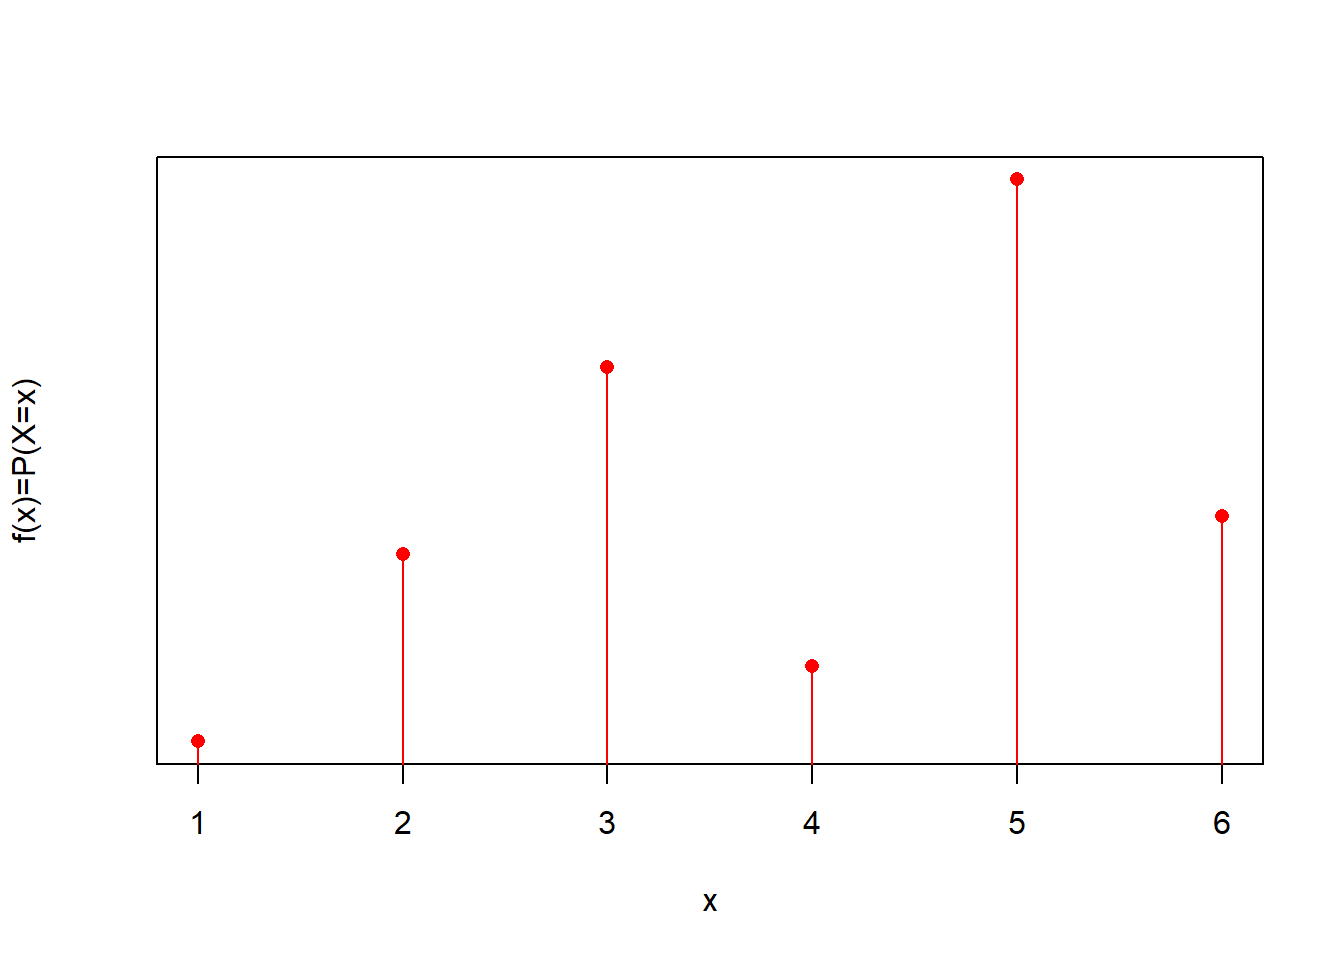
\includegraphics{_main_files/figure-latex/unnamed-chunk-37-1.pdf}

\[\mu =E(X)=\sum_{i=1}^m x_i f(x_i)\]

\(E(X)=\)\textbf{0} * 1/16 + \textbf{1} * 4/16 + \textbf{2} * 6/16 + \textbf{3} * 4/16 + \textbf{4} * 1/16 =2

\begin{center}\rule{0.5\linewidth}{0.5pt}\end{center}

\begin{center}\rule{0.5\linewidth}{0.5pt}\end{center}

\hypertarget{media-y-promedio}{%
\section{Media y Promedio}\label{media-y-promedio}}

\begin{itemize}
\tightlist
\item
  La media \(\mu\) es el centro de gravedad de función de masa de probabilidad y \textbf{no cambia}
\end{itemize}

Por ejemplo de

\begin{longtable}[]{@{}cc@{}}
\toprule
\(X\) & \(P(X=x)\) \\
\midrule
\endhead
\(-2\) & \(1/8=0.125\) \\
\(-1\) & \(2/8=0.25\) \\
\(0\) & \(2/8=0.25\) \\
\(1\) & \(2/8=0.25\) \\
\(2\) & \(1/8=0.125\) \\
\bottomrule
\end{longtable}

\begin{itemize}
\tightlist
\item
  El promedio \(\bar{x}\) es el centro de gravedad de las observaciones (frequencias relativas) \textbf{y cambia} de acuerdo a los datos.
\end{itemize}

Por ejemplo de

\begin{longtable}[]{@{}cc@{}}
\toprule
\(X\) & \(f_i\) \\
\midrule
\endhead
\(-2\) & \(0.132\) \\
\(-1\) & \(0.262\) \\
\(0\) & \(0.240\) \\
\(1\) & \(0.248\) \\
\(2\) & \(0.118\) \\
\bottomrule
\end{longtable}

\begin{center}\rule{0.5\linewidth}{0.5pt}\end{center}

\begin{center}\rule{0.5\linewidth}{0.5pt}\end{center}

\hypertarget{variaciuxf3n}{%
\section{Variación}\label{variaciuxf3n}}

En términos similares definimos la distancia media al cuadrado de la media:

\textbf{Definición}

La varianza, escrita como \(\sigma^2\) o \(V(X)\), de una variable aleatoria discreta \(X\) con función de masa \(f(x)\) está dada por

\[\sigma^2 = V(X)= \sum_{i=1}^M (x_i-\mu)^2 f(x_i)\]

\begin{itemize}
\item
  \(\sigma=\sqrt{V(X)}\) se llama la \textbf{desviación estándar} de la variable aleatoria
\item
  Piense en ello como el momento de inercia de las probabilidades sobre la media.
\end{itemize}

\begin{center}\rule{0.5\linewidth}{0.5pt}\end{center}

\begin{center}\rule{0.5\linewidth}{0.5pt}\end{center}

\hypertarget{ejemplo-varianza}{%
\section{Ejemplo: Varianza}\label{ejemplo-varianza}}

¿Cuál es la varianza de \(X\) si su función de masa de probabilidad \(f(x)\) está dada por

\(P(X=0)=1/16\)
\(P(X=1)=4/16\)
\(P(X=2)=6/16\)
\(P(X=3)=4/16\)
\(P(X=4)=1/16\)

\[\sigma^2 =V(X)=\sum_{i=1}^m (x_i-\mu)^2 f(x_i)\]

\(V(X)=\)\textbf{(0-2)}\(^2\)* 1/16 + \textbf{(1-2)}\(^2\)* 4/16 + \textbf{(2- 2)}\(^2\)* 6/16 + \textbf{(3-2)}\(^2\)* 4/16 + \textbf{(4-2)}\(^2\)* 1/ 16 = 1

\[V(X)=\sigma^2=1\]
\[\sigma=1\]

\begin{center}\rule{0.5\linewidth}{0.5pt}\end{center}

\begin{center}\rule{0.5\linewidth}{0.5pt}\end{center}

\hypertarget{funciones-de-x}{%
\section{\texorpdfstring{Funciones de \(X\)}{Funciones de X}}\label{funciones-de-x}}

\textbf{Definición}

Para cualquier función \(h\) de una variable aleatoria \(X\), con función de masa \(f(x)\), su \textbf{valor esperado} viene dado por

\[ E[h(X)]= \sum_{i=1}^M h(x_i) f(x_i) \]

Esta es una definición importante que nos permite probar \textbf{tres propiedades} importantes de la mediana y la varianza:

\begin{itemize}
\item
  La media de una función lineal es la \textbf{función lineal} de la media: \[E(a\times X +b)= a\times E(X) +b\] para \(a\) y \(b\) escalares (números) .
\item
  La varianza de una función lineal de \(X\) es:\[V(a\times X +b)= a^2\times V(X)\]
\item
  La varianza \textbf{sobre el origen} es la varianza \textbf{sobre la media} más la media al cuadrado: \[E(X^2)=V(X)+E(X)^2\]
\end{itemize}

\begin{center}\rule{0.5\linewidth}{0.5pt}\end{center}

\begin{center}\rule{0.5\linewidth}{0.5pt}\end{center}

\hypertarget{ejemplo-varianza-sobre-el-origen}{%
\section{Ejemplo: Varianza sobre el origen}\label{ejemplo-varianza-sobre-el-origen}}

¿Cuál es la varianza \(X\) sobre el origen, \(E(X^2)\), si su función de masa de probabilidad \(f(x)\) está dada por

\(P(X=0)=1/16\)
\(P(X=1)=4/16\)
\(P(X=2)=6/16\)
\(P(X=3)=4/16\)
\(P(X=4)=1/16\)

\[E(X^2) =\sum_{i=1}^m x_i^2 f(x_i)\]

\(E(X^2)=\)\textbf{(0)}\(^2\)* 1/16 + \textbf{(1)}\(^2\)* 4/16 + \textbf{(2)} \(^2\)* 6/16 + \textbf{(3)}\(^2\)* 4/16 + \textbf{(4)}\(^2\)* 1/16 =5

También podemos verificar:

\[E(X^2)=V(X)+E(X)^2\]

\(5=1+2^2\)

\begin{center}\rule{0.5\linewidth}{0.5pt}\end{center}

\begin{center}\rule{0.5\linewidth}{0.5pt}\end{center}

\hypertarget{distribuciuxf3n-de-probabilidad}{%
\section{Distribución de probabilidad}\label{distribuciuxf3n-de-probabilidad}}

\textbf{Definición:}

La función de \textbf{distribución de probabilidad} se define como

\[F(x)=P(X\leq x)=\sum_{x_i\leq x} f(x_i) \]

Esa es la probabilidad acumulada hasta un valor dado \(x\)

\(F(x)\) satisface:

\begin{itemize}
\tightlist
\item
  \(0\leq F(x) \leq 1\)
\item
  Si \(x \leq y\), entonces \(F(x) \leq F(y)\)
\end{itemize}

\begin{center}\rule{0.5\linewidth}{0.5pt}\end{center}

\begin{center}\rule{0.5\linewidth}{0.5pt}\end{center}

\hypertarget{ejemplo-distribuciuxf3n-de-probabilidad}{%
\section{Ejemplo: distribución de probabilidad}\label{ejemplo-distribuciuxf3n-de-probabilidad}}

Para la función de masa de probabilidad:

\(f(0)=P(X=0)=1/16\)
\(f(1)=P(X=1)=4/16\)
\(f(2)=P(X=2)=6/16\)
\(f(3)=P(X=3)=4/16\)
\(f(4)=P(X=4)=1/16\)

La distribución de probabilidad es:

\[
    F(x)=
\begin{cases}
    1/16,& \text{if } 0 \leq x < 1\\
    5/16,& 1\leq x < 2\\
    11/16,& 2\leq x < 3\\
    15/16,& 4\leq x < 5\\
    16/16,&  x \leq 5\\
\end{cases}
\]

Para \(X \in \mathbb{Z}\)

\begin{center}\rule{0.5\linewidth}{0.5pt}\end{center}

\begin{center}\rule{0.5\linewidth}{0.5pt}\end{center}

\hypertarget{probability-distribution}{%
\section{Probability distribution}\label{probability-distribution}}

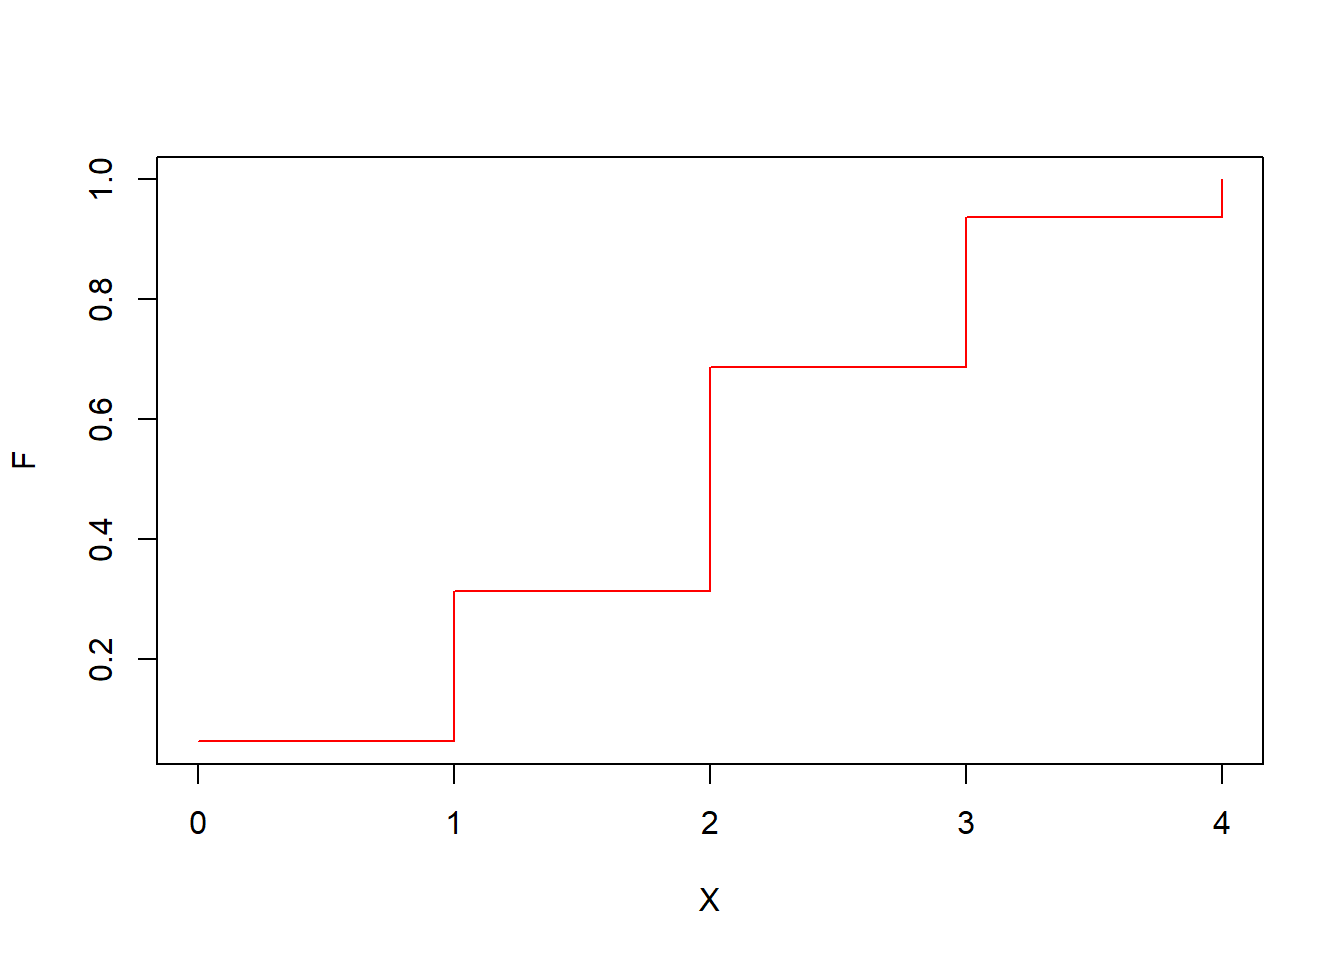
\includegraphics{_main_files/figure-latex/unnamed-chunk-38-1.pdf}

\begin{center}\rule{0.5\linewidth}{0.5pt}\end{center}

\begin{center}\rule{0.5\linewidth}{0.5pt}\end{center}

\hypertarget{funciuxf3n-de-probabilidad-y-distribuciuxf3n-de-probabilidad}{%
\section{Función de probabilidad y Distribución de probabilidad}\label{funciuxf3n-de-probabilidad-y-distribuciuxf3n-de-probabilidad}}

Calcule la función de probabilidad de masa de la siguiente distribución de probabilidad:

\(F(0)=1/16\), \(F(1)=5/16\), \(F(2)=11/16\), \(F(3)=15/16\), \(F(4)= 16/16\),

Trabajemos al revés.

\(f(0)=F(0)=1/16\)
\(f(1)=F(1)-f(0)=5/32-1/32=4/16\)
\(f(2)=F(2)-f(1)-f(0)=F(2)-F(1)=6/16\)
\(f(3)=F(3)-f(2)-f(1)-f(0)=F(3)-F(2)=4/16\)
\(f(4)=F(4)-F(3)=1/16\)

\begin{center}\rule{0.5\linewidth}{0.5pt}\end{center}

\begin{center}\rule{0.5\linewidth}{0.5pt}\end{center}

\hypertarget{funciuxf3n-de-probabilidad-y-distribuciuxf3n-de-probabilidad-1}{%
\section{Función de probabilidad y Distribución de probabilidad}\label{funciuxf3n-de-probabilidad-y-distribuciuxf3n-de-probabilidad-1}}

La distribución de probabilidad es otra forma de especificar la probabilidad de una variable aleatoria.

\[f(x_i)=F(x_i)-F(x_{i-1})\]

con

\[f(x_1)=F(x_1)\]

para \(X\) tomando valores en \(x_1 \leq x_2 \leq ... \leq x_n\)

\begin{center}\rule{0.5\linewidth}{0.5pt}\end{center}

\begin{center}\rule{0.5\linewidth}{0.5pt}\end{center}

\hypertarget{cuantiles}{%
\section{Cuantiles}\label{cuantiles}}

Definimos el \textbf{q-cuantil} como el valor \(x_{p}\) \textbf{bajo} el cual hemos acumulado q*100\% de la probabilidad

\[q=\sum_{i=1}^p f(x_i) = F (x_p)\]

\begin{itemize}
\tightlist
\item
  La \textbf{mediana} es valor \(x_m\) tal que \(q=0.5\)
\end{itemize}

\[F(x_{m})=0.5\]

\begin{itemize}
\tightlist
\item
  El cuantil \(0.05\) es el valor \(x_{r}\) tal que \(q=0.05\)
\end{itemize}

\[F(x_{r})=0.05\]

\begin{itemize}
\tightlist
\item
  El cuantil \(0,25\) es el primer \textbf{cuartil} o sea el valor \(x_{s}\) tal que \(q=0,25\)
\end{itemize}

\[F(x_{s})=0,25\]

\begin{center}\rule{0.5\linewidth}{0.5pt}\end{center}

\begin{center}\rule{0.5\linewidth}{0.5pt}\end{center}

\hypertarget{resumen}{%
\section{Resumen}\label{resumen}}

\begin{longtable}[]{@{}
  >{\centering\arraybackslash}p{(\columnwidth - 4\tabcolsep) * \real{0.43}}
  >{\centering\arraybackslash}p{(\columnwidth - 4\tabcolsep) * \real{0.30}}
  >{\centering\arraybackslash}p{(\columnwidth - 4\tabcolsep) * \real{0.26}}@{}}
\toprule
\begin{minipage}[b]{\linewidth}\centering
nombres de cantidades
\end{minipage} & \begin{minipage}[b]{\linewidth}\centering
modelo (no observado)
\end{minipage} & \begin{minipage}[b]{\linewidth}\centering
datos (observados)
\end{minipage} \\
\midrule
\endhead
función de masa de probabilidad // frecuencia relativa & \(f(x_i)=P(X=x_i)\) & \(f_i=\frac{n_i}{N}\) \\
distribución de probabilidad // frecuencia relativa acumulada & \(F(x_i)=P(X \leq x_i)\) & \(F_i=\sum_{k\leq i} f_k\) \\
media // promedio & \(\mu=E(X)=\sum_{i=1}^M x_i f(x_i)\) & \(\bar{x}=\sum_{j=1}^N x_j/N\) \\
varianza // varianza de la muestra & \(\sigma^2=V(X)=\sum_{i=1}^M (x_i-\mu)^2 f(x_i)\) & \(s^2=\sum_{j=1}^N (x_j-\bar{x})^2/(N-1)\) \\
desviación estándar // muestra sd & \(\sigma=\sqrt{V(X)}\) & \(s\) \\
varianza sobre el origen // 2º momento muestral & \(E(X^2)=\sum_{i=1}^M x_i^2 f(x_i)\) & \(m_2= \sum_{j=1}^N x_j^2/n\) \\
\bottomrule
\end{longtable}

Tenga en cuenta que:

\begin{itemize}
\tightlist
\item
  \(i=1...M\) es un \textbf{resultado} de la variable aleatoria \(X\).
\item
  \(j=1...N\) es una \textbf{observación} de la variable aleatoria \(X\).
\end{itemize}

Propiedades:

\begin{itemize}
\tightlist
\item
  \(\sum_{i=1...N} f(x_i)=1\)
\item
  \(f(x_i)=F(x_i)-F(x_{i-1})\)
\item
  \(E(a\times X +b)= a\times E(X) +b\); para los escalares \(a\) y \(b\).
\item
  \(V(a\times X +b)= a^2\times V(X)\)
\item
  \(E(X^2)=V(X)+E(X)^2\)
\end{itemize}

\hypertarget{variables-aleatorias-continuas}{%
\chapter{Variables aleatorias continuas}\label{variables-aleatorias-continuas}}

\hypertarget{objetivo-5}{%
\section{Objetivo}\label{objetivo-5}}

\begin{itemize}
\tightlist
\item
  Función de densidad de probabilidad
\item
  Media y varianza
\item
  Distribución de probabilidad
\end{itemize}

\begin{center}\rule{0.5\linewidth}{0.5pt}\end{center}

\begin{center}\rule{0.5\linewidth}{0.5pt}\end{center}

\hypertarget{variable-aleatoria-continua}{%
\section{Variable aleatoria continua}\label{variable-aleatoria-continua}}

¿Qué sucede con las variables aleatorias continuas?

Reconsideremos el ángulo de convexidad de los pacientes con misofonía (Sección 2.21).

\begin{itemize}
\tightlist
\item
  Para esta variabler redefinimos los resultados como pequeños intervalos regulares (bins) y calculamos la frecuencia relativa para cada uno de ellos como hicimos en el caso discreto.
\end{itemize}

\begin{verbatim}
##        outcome ni         fi
## 1 [-1.02,3.46]  8 0.06504065
## 2  (3.46,7.92] 51 0.41463415
## 3  (7.92,12.4] 26 0.21138211
## 4  (12.4,16.8] 20 0.16260163
## 5  (16.8,21.3] 18 0.14634146
\end{verbatim}

\begin{center}\rule{0.5\linewidth}{0.5pt}\end{center}

\begin{center}\rule{0.5\linewidth}{0.5pt}\end{center}

\hypertarget{variable-aleatoria-continua-1}{%
\section{Variable aleatoria continua}\label{variable-aleatoria-continua-1}}

Consideremos nuevamente que sus frecuencias relativas son las probabilidades cuando \(N \rightarrow \infty\)

\[f_i=\frac{n_i}{N} \rightarrow f(x_i)=P(X=x_i)\]

La probabilidad depende ahora de la longitud de los bins \(\Delta x\). Si hacemos los contenedores cada vez más pequeños, las frecuencias se hacen más pequeñas y, por lo tanto,

\(P(X=x_i) \rightarrow 0\) cuando \(\Delta x \rightarrow 0\), porque \(n_i \rightarrow 0\)

\begin{verbatim}
##          outcome ni         fi
## 1  [-1.02,0.115]  2 0.01626016
## 2   (0.115,1.23]  0 0.00000000
## 3    (1.23,2.34]  3 0.02439024
## 4    (2.34,3.46]  3 0.02439024
## 5    (3.46,4.58]  2 0.01626016
## 6    (4.58,5.69]  4 0.03252033
## 7     (5.69,6.8] 11 0.08943089
## 8     (6.8,7.92] 34 0.27642276
## 9    (7.92,9.04] 12 0.09756098
## 10   (9.04,10.2]  4 0.03252033
## 11   (10.2,11.3]  3 0.02439024
## 12   (11.3,12.4]  7 0.05691057
## 13   (12.4,13.5]  2 0.01626016
## 14   (13.5,14.6]  6 0.04878049
## 15   (14.6,15.7]  4 0.03252033
## 16   (15.7,16.8]  8 0.06504065
## 17     (16.8,18]  4 0.03252033
## 18     (18,19.1]  9 0.07317073
## 19   (19.1,20.2]  3 0.02439024
## 20   (20.2,21.3]  2 0.01626016
\end{verbatim}

\begin{center}\rule{0.5\linewidth}{0.5pt}\end{center}

\begin{center}\rule{0.5\linewidth}{0.5pt}\end{center}

\hypertarget{variable-aleatoria-continua-2}{%
\section{Variable aleatoria continua}\label{variable-aleatoria-continua-2}}

Definimos una cantidad en un punto \(x\) que es la cantidad de probabilidad por unidad de distancia que encontraríamos en un contenedor \textbf{infinitesimal} \(dx\) en \(x\)

\[f(x)= \frac{P(x\leq X \leq x+dx)}{dx}\]

\(f(x)\) se llama la función de \textbf{densidad} de probabilidad.

Por tanto, la probabilidad de observar \(x\) entre \(x\) y \(x+dx\)
está dada por

\[P(x\leq X \leq x+dx)= f(x) dx\]

\begin{center}\rule{0.5\linewidth}{0.5pt}\end{center}

\begin{center}\rule{0.5\linewidth}{0.5pt}\end{center}

\hypertarget{variable-aleatoria-continua-3}{%
\section{Variable aleatoria continua}\label{variable-aleatoria-continua-3}}

\textbf{Definición}

Para una variable aleatoria continua \(X\), una función de \textbf{densidad de probabilidad} es tal que

La función es positiva:

\begin{itemize}
\tightlist
\item
  \(f(x) \geq 0\)
\end{itemize}

La probabilidad de observar un valor dentro de un intervalo es el \textbf{área bajo la curva}:

\begin{itemize}
\tightlist
\item
  \(P(a\leq X \leq b)=\int_{a}^{b} f(x) dx\)
\end{itemize}

La probabilidad de observar \textbf{cualquier} valor es 1:

\begin{itemize}
\tightlist
\item
  \(\int_{-\infty}^{\infty} f(x) dx = 1\)
\end{itemize}

\begin{center}\rule{0.5\linewidth}{0.5pt}\end{center}

\begin{center}\rule{0.5\linewidth}{0.5pt}\end{center}

\hypertarget{variable-aleatoria-continua-4}{%
\section{Variable aleatoria continua}\label{variable-aleatoria-continua-4}}

\begin{itemize}
\item
  La función de densidad de probabilidad es un paso adelante en la abstracción de probabilidades: sumamos el límite continuo (\(dx \rightarrow 0\)).
\item
  Todas las propiedades de las probabilidades se traducen en términos de densidades (\(\sum \rightarrow \int\)).
\item
  La asignación de probabilidades a una variable aleatoria se puede realizar con argumentos de equiprobabilidad (clásicos).
\item
  Las densidades son cantidades matemáticas que algunas asignarán a experimentos y otras no. \emph{¿Qué densidad corresponderá mejor a mi experimento?}
\end{itemize}

\begin{center}\rule{0.5\linewidth}{0.5pt}\end{center}

\begin{center}\rule{0.5\linewidth}{0.5pt}\end{center}

\hypertarget{uxe1rea-total-bajo-la-curva}{%
\section{Área total bajo la curva}\label{uxe1rea-total-bajo-la-curva}}

Ejemplo: toma la \textbf{densidad de probabilidad} que podría describir la variable aleatoria que mide dónde cae una gota de lluvia en una canaleta de lluvia de \(100cm\) de longitud.

\[
    f(x)= 
\begin{cases}
    \frac{1}{100},& \text{si } x\in (0,100)\\
    0,& si \, no 
\end{cases}
\]

Entonces la probabilidad de \textbf{cualquier} observación es el \textbf{área total bajo la curva}

\(P(-\infty\leq X \leq \infty)= \int_{-\infty}^{\infty} f(x) dx = 100*0.01= 1\)

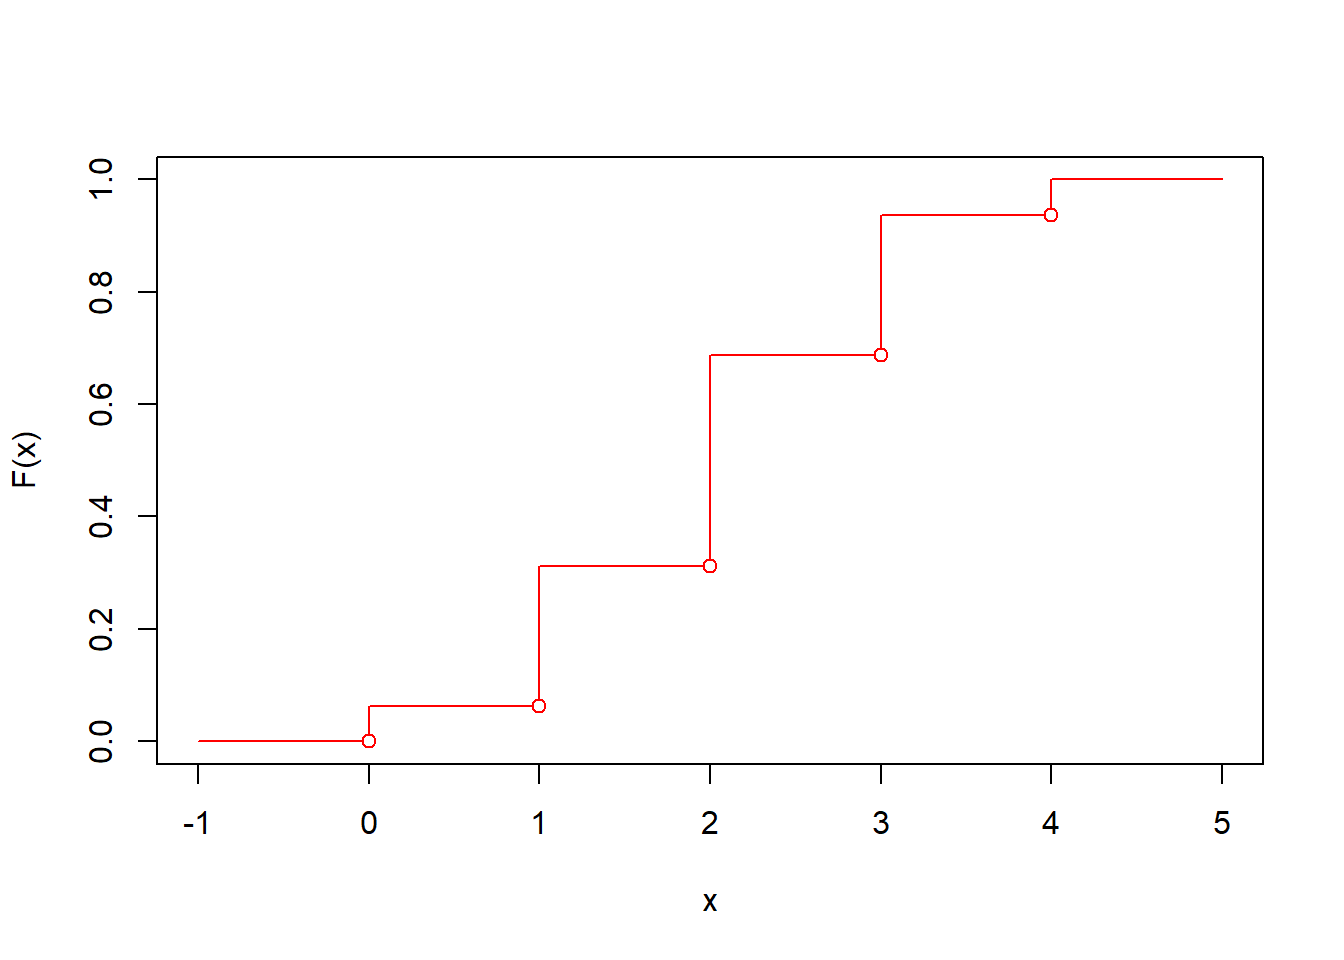
\includegraphics{_main_files/figure-latex/unnamed-chunk-41-1.pdf}

\begin{center}\rule{0.5\linewidth}{0.5pt}\end{center}

\begin{center}\rule{0.5\linewidth}{0.5pt}\end{center}

\hypertarget{uxe1rea-bajo-la-curva}{%
\section{Área bajo la curva}\label{uxe1rea-bajo-la-curva}}

La probabilidad de observar \(x\) en un intervalo es el \textbf{área bajo la curva} dentro del intervalo

\begin{itemize}
\tightlist
\item
  \(P(20 \leq X \leq 60) = \int_{20}^{60} f(x) dx = (60-20)*0.01=0.4\)
\end{itemize}

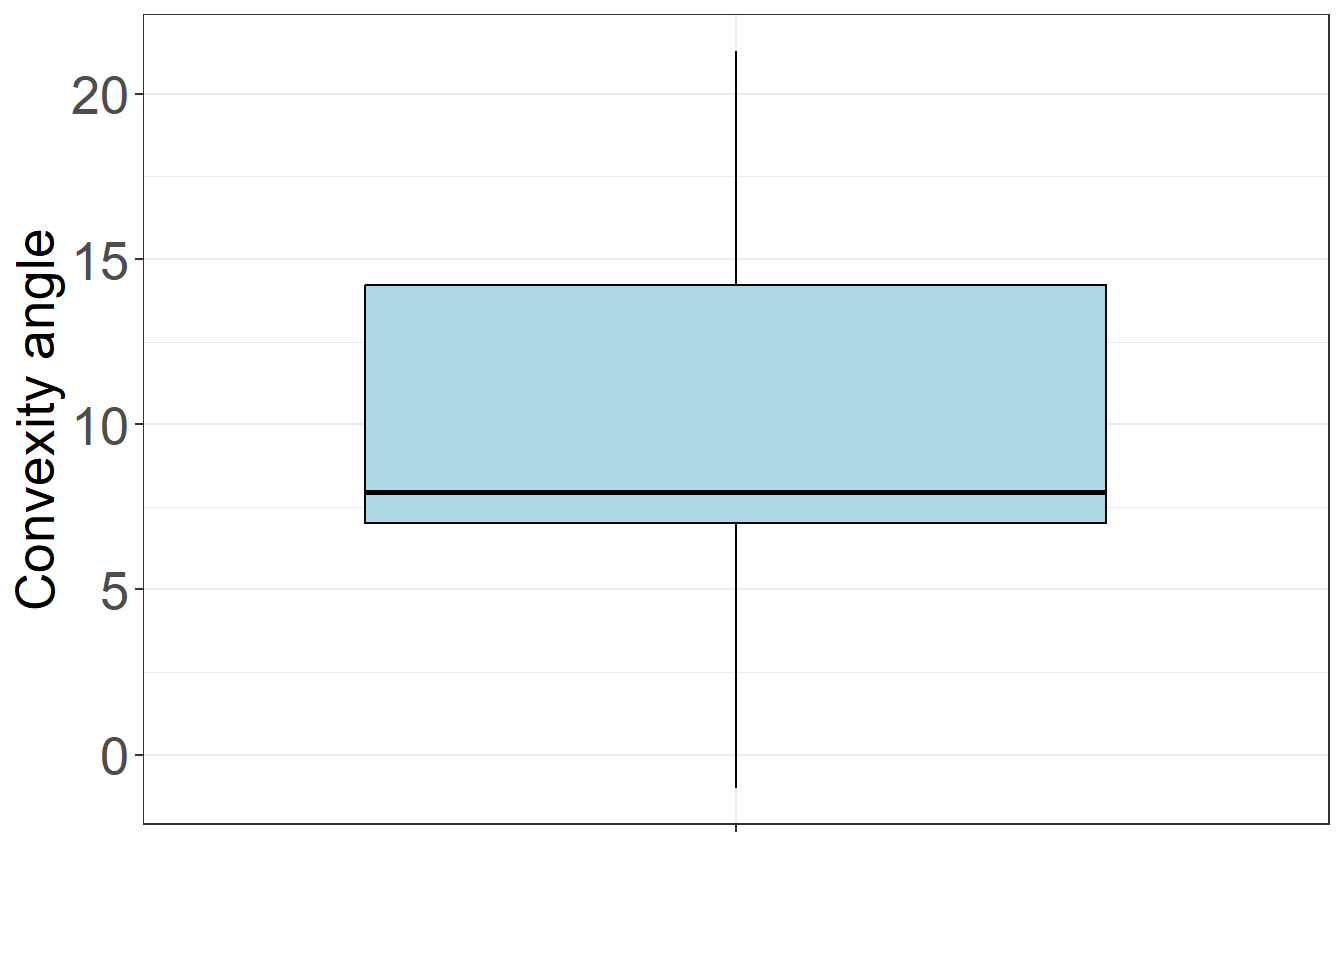
\includegraphics{_main_files/figure-latex/unnamed-chunk-42-1.pdf}

\begin{center}\rule{0.5\linewidth}{0.5pt}\end{center}

\begin{center}\rule{0.5\linewidth}{0.5pt}\end{center}

\hypertarget{uxe1rea-bajo-la-curva-1}{%
\section{Área bajo la curva}\label{uxe1rea-bajo-la-curva-1}}

En general, \(f(x)\) debe satisfacer:

\begin{itemize}
\tightlist
\item
  \(0 \leq P(a \leq X \leq b) = \int_{a}^{b} f(x) dx \leq 1\)
\end{itemize}

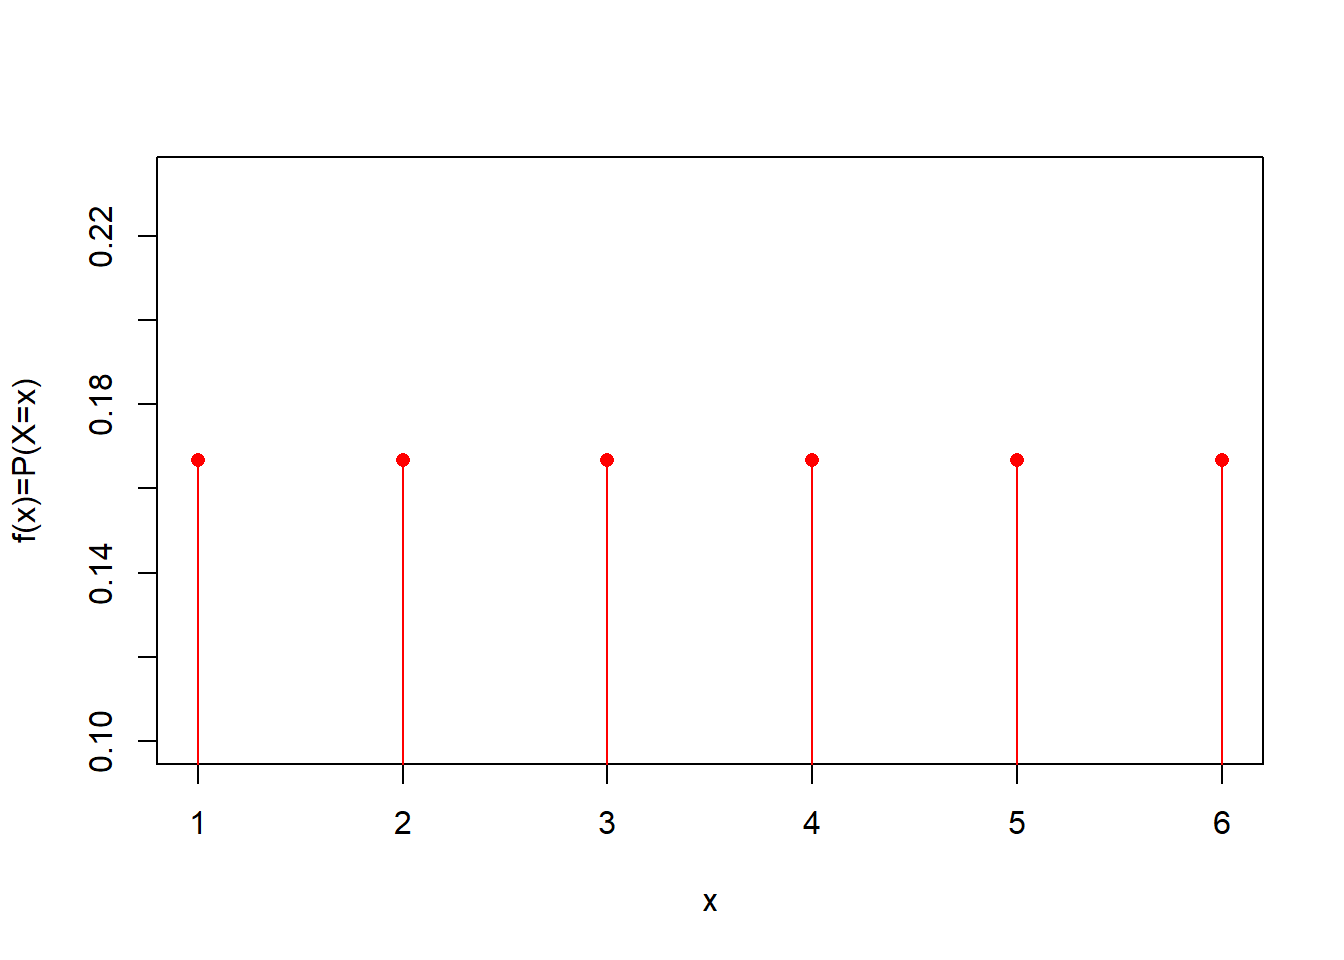
\includegraphics{_main_files/figure-latex/unnamed-chunk-43-1.pdf}

\begin{center}\rule{0.5\linewidth}{0.5pt}\end{center}

\begin{center}\rule{0.5\linewidth}{0.5pt}\end{center}

\hypertarget{distribuciuxf3n-de-probabilidad-1}{%
\section{Distribución de probabilidad}\label{distribuciuxf3n-de-probabilidad-1}}

La probabilidad acumulada hasta \(b\) está definida por la distribución de probabilidad \(F\)

\begin{itemize}
\tightlist
\item
  \(F(b) = P(X \leq b)=\int_{-\infty}^bf(x)dx\)
\end{itemize}

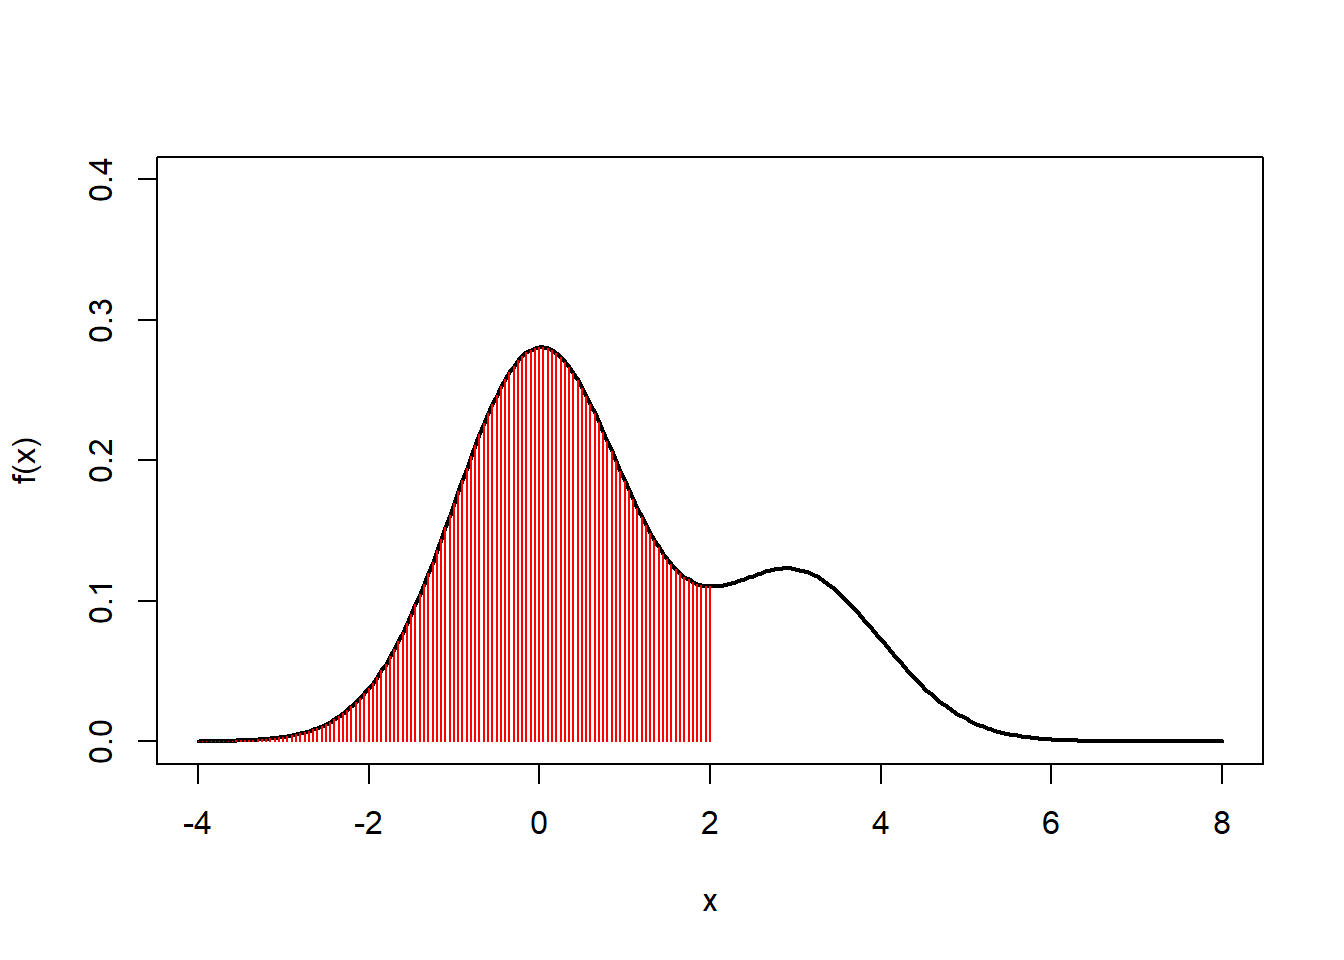
\includegraphics{_main_files/figure-latex/unnamed-chunk-44-1.pdf}

La probabilidad acumulada hasta \(a\) es

\begin{itemize}
\tightlist
\item
  \(F(a) = P(X \leq a)\)
\end{itemize}

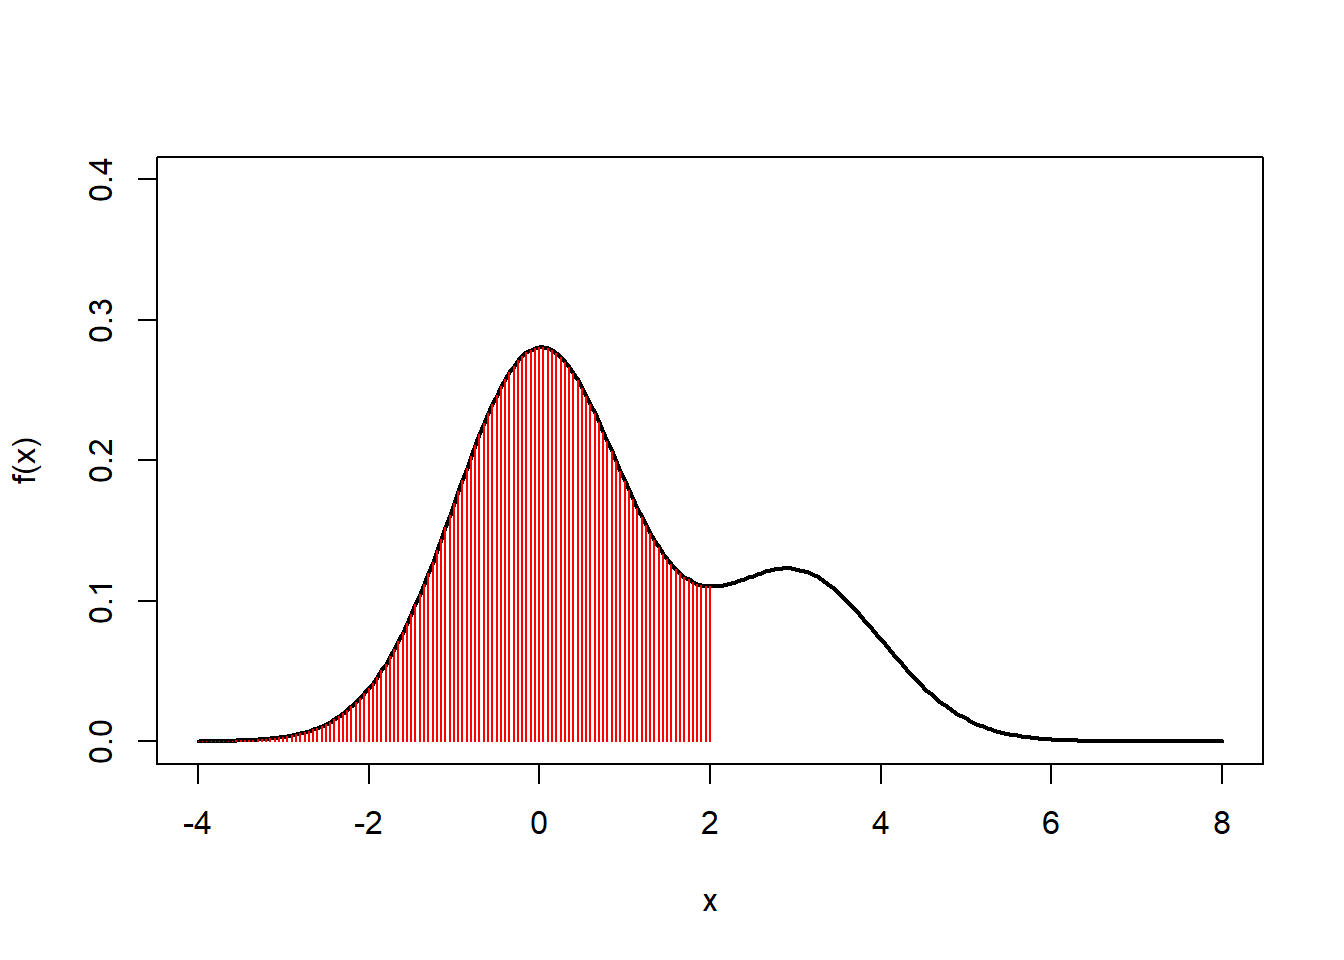
\includegraphics{_main_files/figure-latex/unnamed-chunk-45-1.pdf}

\begin{center}\rule{0.5\linewidth}{0.5pt}\end{center}

\begin{center}\rule{0.5\linewidth}{0.5pt}\end{center}

\hypertarget{distribuciuxf3n-de-probabilidad-2}{%
\section{Distribución de probabilidad}\label{distribuciuxf3n-de-probabilidad-2}}

La probabilidad entre \(a\) y \(b\) está definida por la distribución de probabilidad \(F\)

\begin{itemize}
\tightlist
\item
  \(P(a\leq X \leq b) = \int_a^b f(x)dx=F(b)-F(a)\)
\end{itemize}

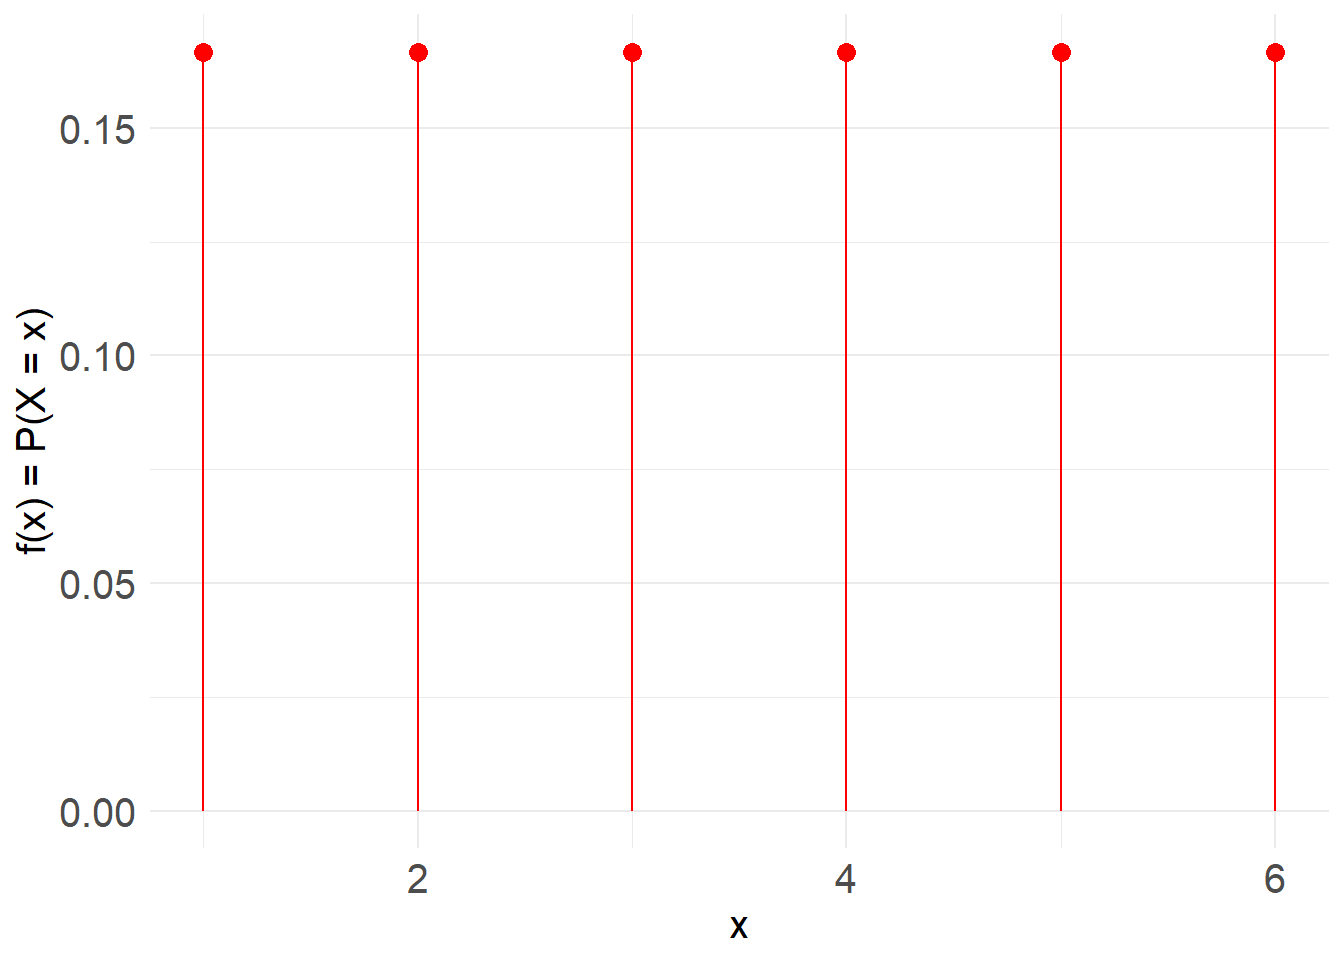
\includegraphics{_main_files/figure-latex/unnamed-chunk-46-1.pdf}

\begin{center}\rule{0.5\linewidth}{0.5pt}\end{center}

\begin{center}\rule{0.5\linewidth}{0.5pt}\end{center}

\hypertarget{distribuciuxf3n-de-probabilidad-3}{%
\section{Distribución de probabilidad}\label{distribuciuxf3n-de-probabilidad-3}}

La distribución de probabilidad de una variable aleatoria continua se define como
\(F(a)=P(X\leq a) =\int_{-\infty} ^a f(x)dx\)

con las propiedades que:

Está entre \(0\) y \(1\):

\begin{itemize}
\tightlist
\item
  \(F(-\infty)= 0\) y \(F(\infty)=1\)
\end{itemize}

Siempre aumenta:

\begin{itemize}
\tightlist
\item
  si \(a\leq b\) entonces \(F(a)\leq F(b)\)
\end{itemize}

Se puede utilizar para calcular probabilidades:

\begin{itemize}
\tightlist
\item
  \(P(a \leq X \leq b)=F(b)-F(a)\)
\end{itemize}

Recupera la densidad de probabilidad:

\begin{itemize}
\tightlist
\item
  \(f(x)=\frac{dF(x)}{dx}\)
\end{itemize}

Usamos \textbf{distribuciones de probabilidad} para \textbf{calcular probabilidades} de una variable aleatoria en intervalos

\begin{center}\rule{0.5\linewidth}{0.5pt}\end{center}

\begin{center}\rule{0.5\linewidth}{0.5pt}\end{center}

\hypertarget{distribuciuxf3n-de-probabilidad-4}{%
\section{Distribución de probabilidad}\label{distribuciuxf3n-de-probabilidad-4}}

Para la funcion de densidad uniforme:

\[
    f(x)= 
\begin{cases}
    \frac{1}{100},& \text{si } x\in (0,100)\\
    0,& si \,no 
\end{cases}
\]

La distribución de probabilidad es

\[
    F(a)= 
\begin{cases}
    0,& a \leq 0 \\
    \frac{a}{100},& \text{si } a\in [0,100)\\
    1, & 100 < a \\
    \\
\end{cases}
\]

\begin{center}\rule{0.5\linewidth}{0.5pt}\end{center}

\begin{center}\rule{0.5\linewidth}{0.5pt}\end{center}

\hypertarget{gruxe1ficos-de-probabilidad}{%
\section{Gráficos de probabilidad}\label{gruxe1ficos-de-probabilidad}}

La probabilidad \(P(20<X<60)\) es el \emph{área} bajo la curva de \textbf{densidad}

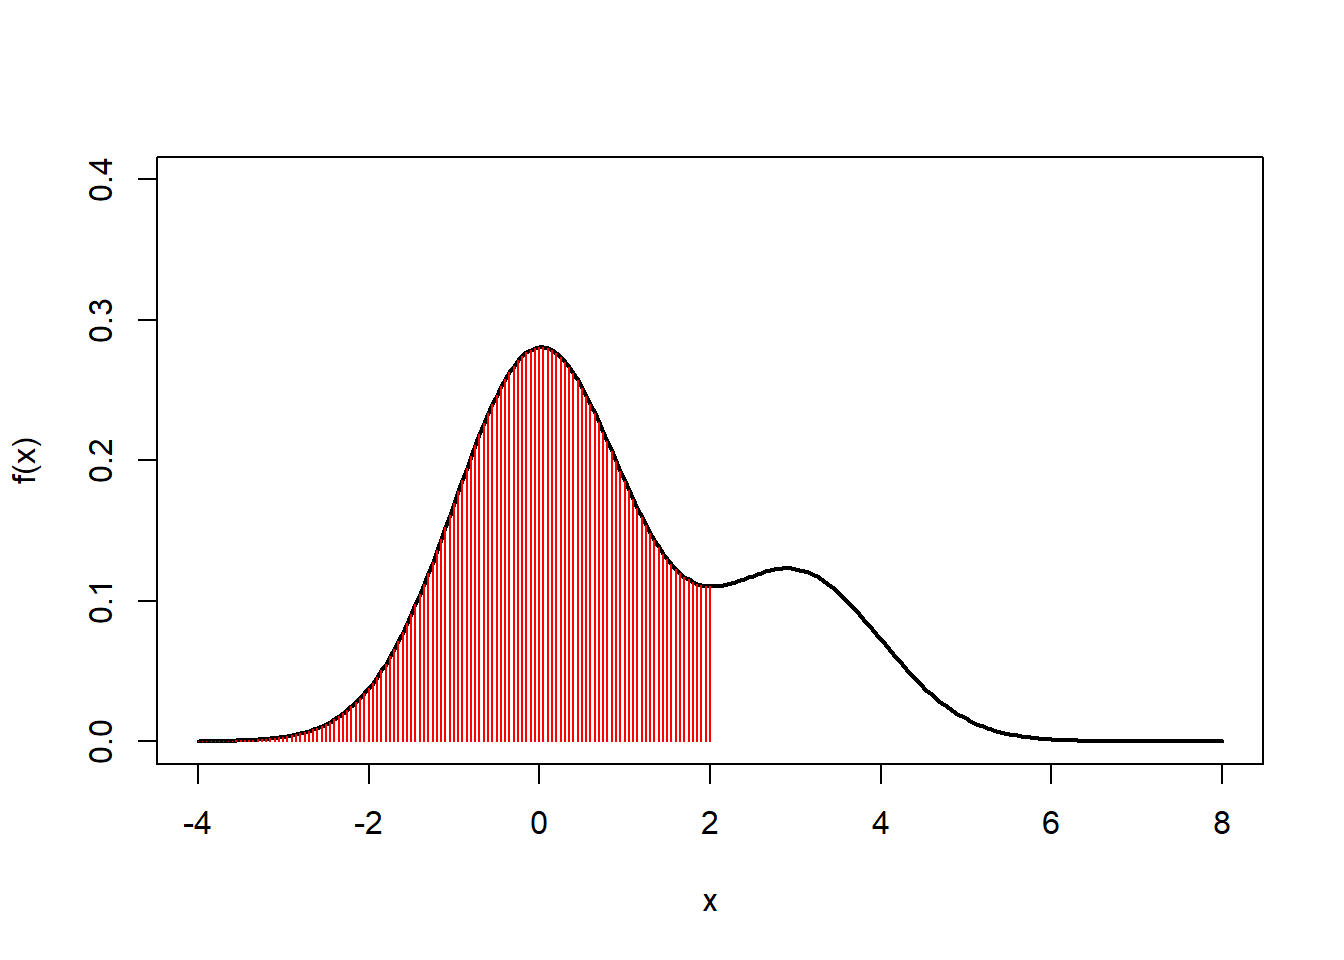
\includegraphics{_main_files/figure-latex/unnamed-chunk-47-1.pdf}

\begin{center}\rule{0.5\linewidth}{0.5pt}\end{center}

\begin{center}\rule{0.5\linewidth}{0.5pt}\end{center}

\hypertarget{gruxe1ficos-de-probabilidad-1}{%
\section{Gráficos de probabilidad}\label{gruxe1ficos-de-probabilidad-1}}

La probabilidad \(P(20<X<60)\) es la \emph{diferencia} en valores de \textbf{distribución}

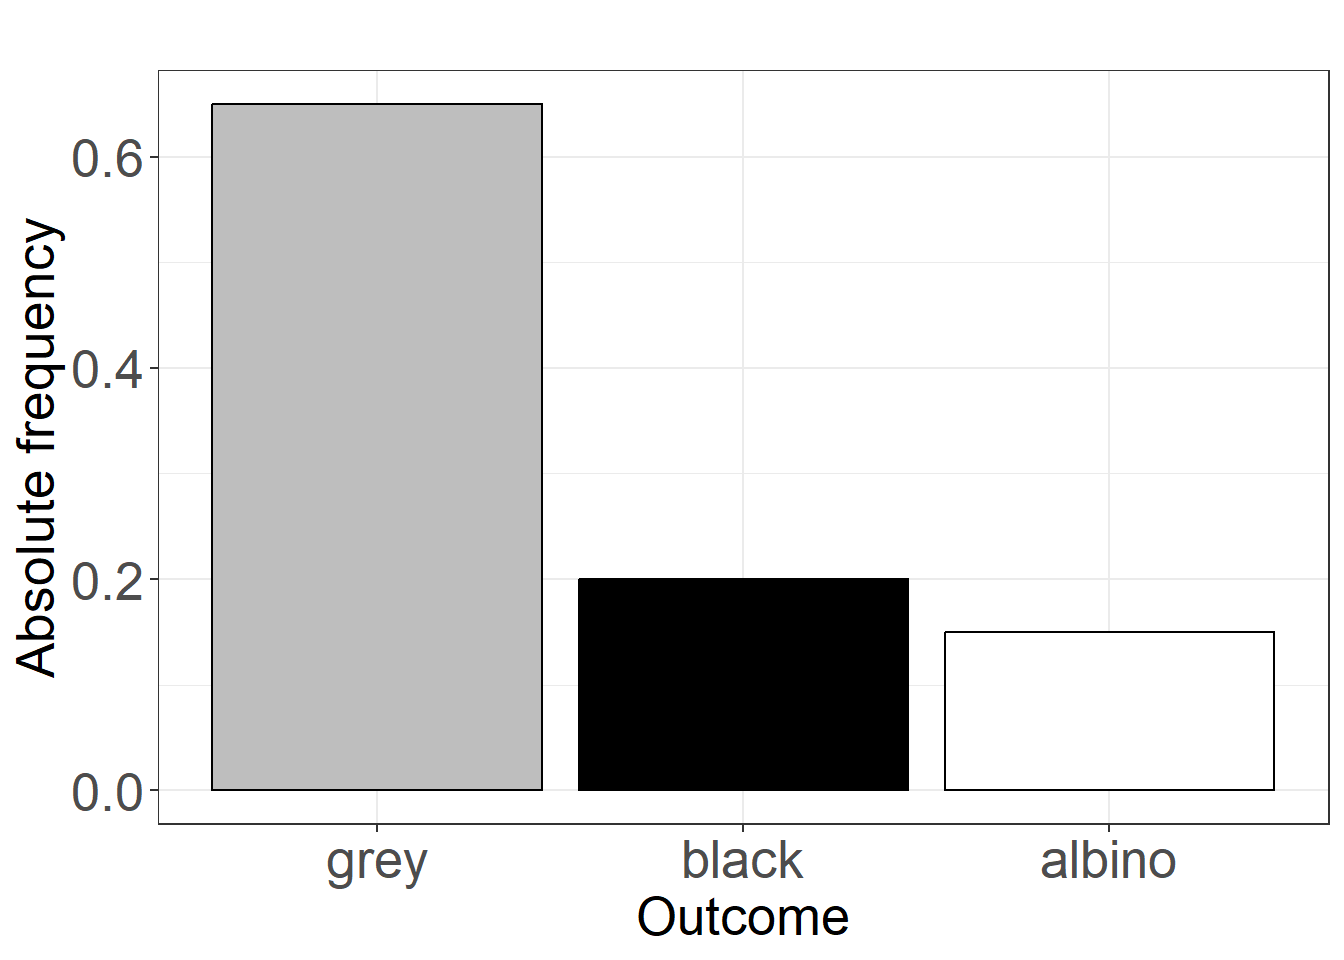
\includegraphics{_main_files/figure-latex/unnamed-chunk-48-1.pdf}

\begin{center}\rule{0.5\linewidth}{0.5pt}\end{center}

\begin{center}\rule{0.5\linewidth}{0.5pt}\end{center}

\hypertarget{media-1}{%
\section{Media}\label{media-1}}

Como en el caso discreto, la \textbf{media} mide el centro de la distribución

\textbf{Definición}

Supongamos que \(X\) es una variable aleatoria continua con función de probabilidad \textbf{densidad} \(f(x)\). El valor medio o esperado de \(X\), denotado como \(\mu\) o \(E(X)\), es

\[\mu=E(X)=\int_{-\infty}^\infty x f(x) dx\]
Es la versión continua del centro de masa.

\begin{center}\rule{0.5\linewidth}{0.5pt}\end{center}

\begin{center}\rule{0.5\linewidth}{0.5pt}\end{center}

\hypertarget{media-2}{%
\section{Media}\label{media-2}}

\[
    f(x)= 
\begin{cases}
    \frac{1}{100},& \text{si } x\in (0,100)\\
    0,& si \, no 
\end{cases}
\]

\(E(X)=50\)

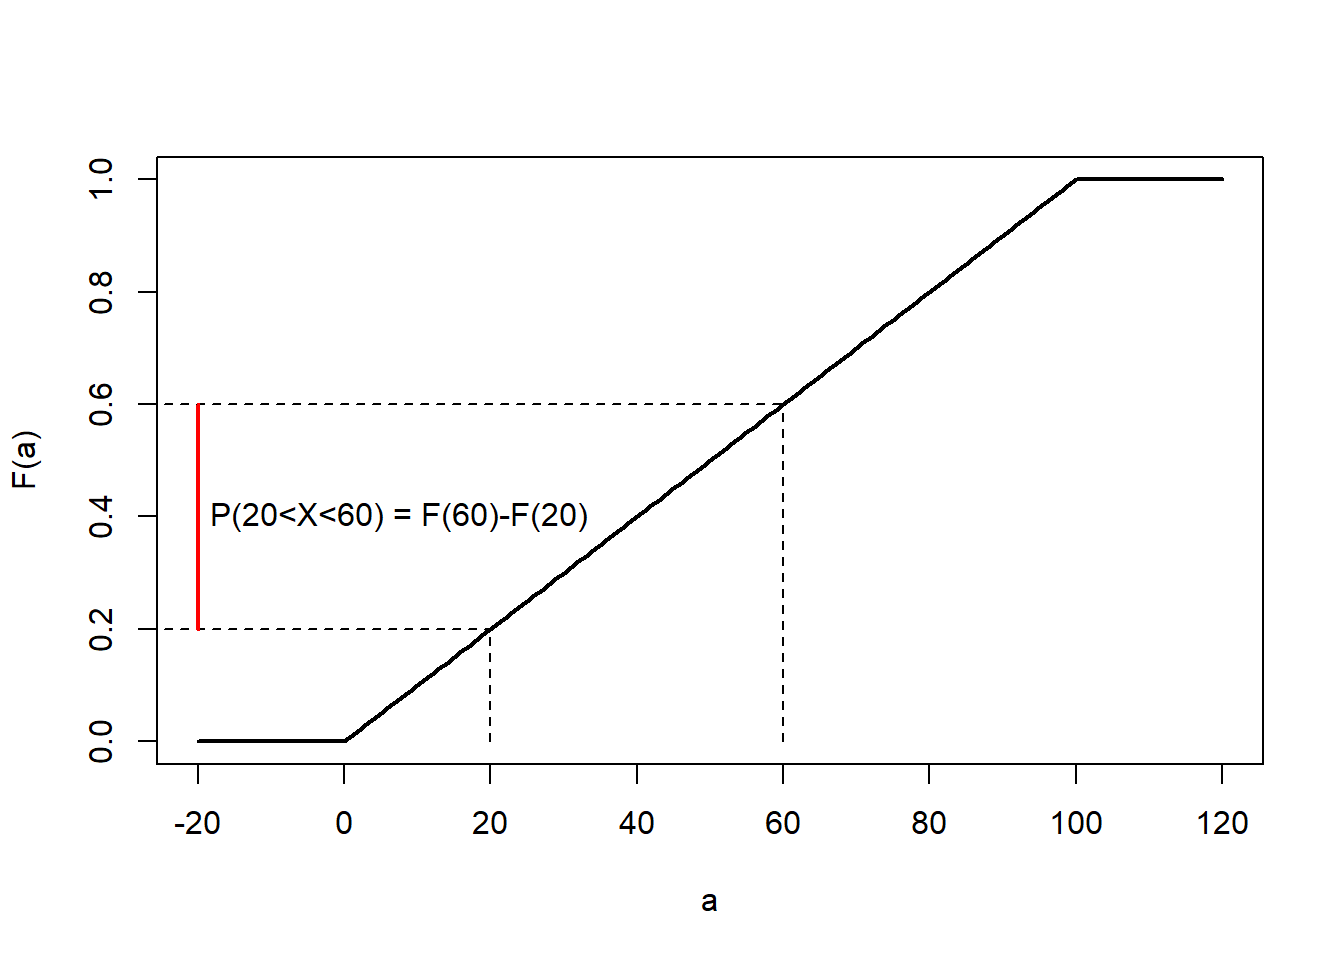
\includegraphics{_main_files/figure-latex/unnamed-chunk-49-1.pdf}

\begin{center}\rule{0.5\linewidth}{0.5pt}\end{center}

\begin{center}\rule{0.5\linewidth}{0.5pt}\end{center}

\hypertarget{varianza}{%
\section{Varianza}\label{varianza}}

Como en el caso discreto, la varianza mide la dispersión con respecto a la media

\textbf{Definición}

Supongamos que \(X\) es una variable aleatoria continua con función de densidad de probabilidad \(f(x)\). La varianza de \(X\), denotada como \(\sigma^2\) o \(V(X)\), es

\[\sigma^2=V(X)=\int_{-\infty}^\infty (x-\mu)^2 f(x) dx\]

\begin{center}\rule{0.5\linewidth}{0.5pt}\end{center}

\begin{center}\rule{0.5\linewidth}{0.5pt}\end{center}

\hypertarget{funciones-de-x-1}{%
\section{\texorpdfstring{Funciones de \(X\)}{Funciones de X}}\label{funciones-de-x-1}}

\textbf{Definición}

Para cualquier función \(h\) de una variable aleatoria \(X\), con función de masa \(f(x)\), su valor esperado viene dado por

\[E[h(X)]= \int_{-\infty}^{\infty} h(x) f(x)dx\]

Y tenemos las mismas propiedades que en el caso discreto

\begin{itemize}
\item
  La media de una función lineal es la función lineal de la media: \[E(a\times X +b)= a\times E(X) +b\] para \(a\) y \(b\) escalares.
\item
  La varianza de una función lineal de \(X\) es:\[V(a\times X +b)= a^2\times V(X)\]
\item
  La varianza sobre el origen es la varianza sobre la media más la media al cuadrado: \[E(X^2)=V(X)+E(X)^2\]
\end{itemize}

\begin{center}\rule{0.5\linewidth}{0.5pt}\end{center}

\begin{center}\rule{0.5\linewidth}{0.5pt}\end{center}

\hypertarget{ejemplo-8}{%
\section{Ejemplo}\label{ejemplo-8}}

\begin{itemize}
\tightlist
\item
  para la densidad de probabilidad
\end{itemize}

\[
    f(x)= 
\begin{cases}
    \frac{1}{100},& \text{si } x\in (0,100)\\
    0,& si \, no 
\end{cases}
\]

\begin{itemize}
\tightlist
\item
  calcule la media
\item
  calcule la varianza usando \(E(X^2)=V(X)+E(X)^2\)
\item
  calcule \(P(\mu-\sigma\leq X \leq \mu+\sigma)\)
\item
  ¿Cuáles son el primer y tercer cuartiles?
\end{itemize}

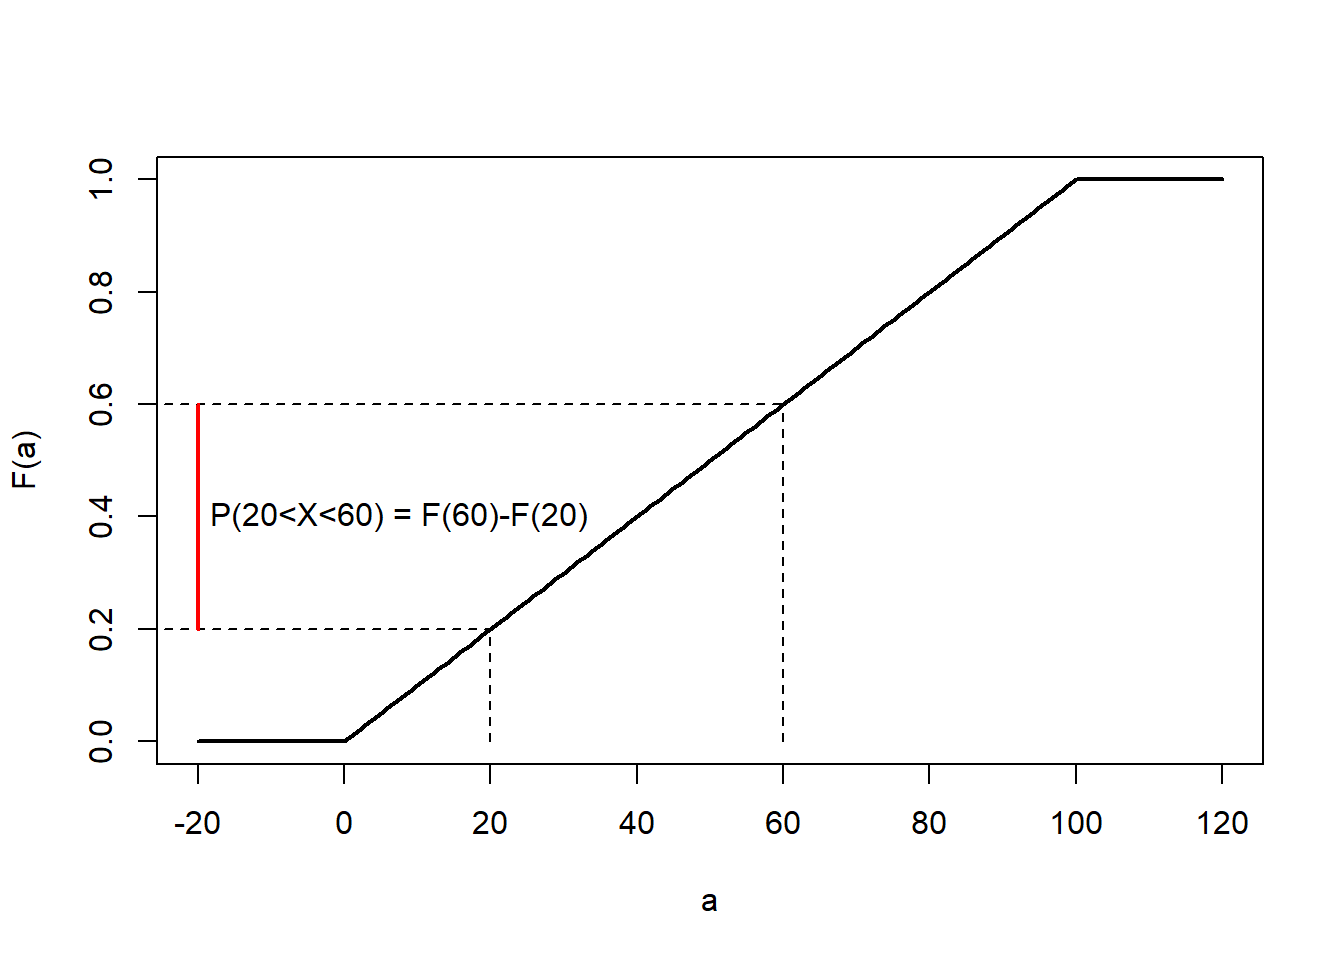
\includegraphics{_main_files/figure-latex/unnamed-chunk-50-1.pdf}

\hypertarget{modelos-de-probabilidad-para-variables-aleatorias-discretas}{%
\chapter{Modelos de probabilidad para variables aleatorias discretas}\label{modelos-de-probabilidad-para-variables-aleatorias-discretas}}

\hypertarget{objetivo-6}{%
\section{Objetivo}\label{objetivo-6}}

Modelos probabilidad:

\begin{itemize}
\tightlist
\item
  Funciones de probabilidad uniforme y de Bernoulli
\item
  Funciones de probabilidad binomial y binomial negativa
\end{itemize}

\begin{center}\rule{0.5\linewidth}{0.5pt}\end{center}

\begin{center}\rule{0.5\linewidth}{0.5pt}\end{center}

\hypertarget{funciuxf3n-de-probabilidad}{%
\section{Función de probabilidad}\label{funciuxf3n-de-probabilidad}}

Una función de masa de probabilidad de una \textbf{variable aleatoria discreta} \(X\) con valores posibles \(x_1 , x_2 , .. , x_M\) es \textbf{cualquier función} tal que

es positiva:

\begin{itemize}
\tightlist
\item
  \(f(x_i)\geq 0\)
\end{itemize}

\emph{Nos permite calcular probabilidades:}

\begin{itemize}
\tightlist
\item
  \(f(x_i)=P(X=x_i)\)
\end{itemize}

La probabilidad de observar algún resultado es \(1\)

\begin{itemize}
\tightlist
\item
  \(\sum_{i=1}^M f(x_i)=1\)
\end{itemize}

\textbf{Propiedades:}

Tendencia central:

\begin{itemize}
\tightlist
\item
  \(E(X)= \sum_{i=1}^M x_i f(x_i)\)
\end{itemize}

Dispersión:

\begin{itemize}
\tightlist
\item
  \(V(X)= \sum_{i=1}^M (x_i-\mu)^2 f(x_i)\)
\end{itemize}

Son objetos abstractos con propiedades generales que pueden o no \textbf{describir} un proceso natural o de ingeniería.

\begin{center}\rule{0.5\linewidth}{0.5pt}\end{center}

\begin{center}\rule{0.5\linewidth}{0.5pt}\end{center}

\hypertarget{modelo-de-probabilidad}{%
\section{Modelo de probabilidad}\label{modelo-de-probabilidad}}

Un \textbf{modelo de probabilidad} es una función de masa de probabilidad que puede representar las probabilidades de un experimento aleatorio.

\textbf{Ejemplos:}

\begin{itemize}
\item
  \(f(x)=P(X=x)=1/6\) representa la probabilidad de los resultados de \textbf{una} tirada de dados.
\item
  La función de masa de probabilidad
\end{itemize}

\begin{longtable}[]{@{}cc@{}}
\toprule
\(X\) & \(f(x)\) \\
\midrule
\endhead
\(-2\) & \(1/8\) \\
\(-1\) & \(2/8\) \\
\(0\) & \(2/8\) \\
\(1\) & \(2/8\) \\
\(2\) & \(1/8\) \\
\bottomrule
\end{longtable}

Representa la probabilidad de sacar \textbf{una} bola de una urna donde hay dos bolas por etiqueta: \(-1, 0, 1\) y una bola por etiqueta: \(-2, 2\).

\begin{center}\rule{0.5\linewidth}{0.5pt}\end{center}

\begin{center}\rule{0.5\linewidth}{0.5pt}\end{center}

\hypertarget{modelos-paramuxe9tricos}{%
\section{Modelos paramétricos}\label{modelos-paramuxe9tricos}}

Cuando realizamos un experimento aleatorio y \textbf{no} sabemos las probabilidades de los resultados:

\begin{itemize}
\tightlist
\item
  Siempre podemos formular el modelo dado por las frecuencias relativas: \(\hat{P}(X=x_i)=f_i\) (donde \(i=1...M\)).
\end{itemize}

Necesitamos encontrar \(M\) números cada uno dependiendo de \(N\).

En muchos casos:

\begin{itemize}
\tightlist
\item
  Podemos formular funciones de probabilidad \(f(x)\) que dependen solamente de \textbf{muy pocos} números.
\end{itemize}

\textbf{Ejemplo:}

Un experimento aleatorio con \(M\) resultados igualmente probables tiene una función de masa de probabilidad:
\[f(x)=P(X=x)=1/M\]

Solo necesitamos saber \(M\).

Los números que \textbf{necesitamos saber} para determinar completamente una función de probabilidad se llaman \textbf{parámetros}.

\begin{center}\rule{0.5\linewidth}{0.5pt}\end{center}

\begin{center}\rule{0.5\linewidth}{0.5pt}\end{center}

\hypertarget{distribuciuxf3n-uniforme-un-paruxe1metro}{%
\section{Distribución uniforme (un parámetro)}\label{distribuciuxf3n-uniforme-un-paruxe1metro}}

\textbf{Definición}
Una variable aleatoria \(X\) con resultados \(\{1,...M\}\) tiene una \textbf{distribución uniforme} discreta si todos sus resultados \(M\) tienen la misma probabilidad

\[f(x)=\frac{1}{M}\]

Con media y varianza:

\(E(X)= \frac{M+1}{2}\)

\(V(X)= \frac{M^2-1}{12}\)

Nota: \(E(X)\) y \(V(X)\) también son \textbf{parámetros}. Si conocemos alguno de ellos, entonces podemos determinar completamente la distribución.

\[f(x)=\frac{1}{2E(X)-1}\]

\begin{center}\rule{0.5\linewidth}{0.5pt}\end{center}

\begin{center}\rule{0.5\linewidth}{0.5pt}\end{center}

\hypertarget{distribuciuxf3n-uniforme}{%
\section{Distribución uniforme}\label{distribuciuxf3n-uniforme}}

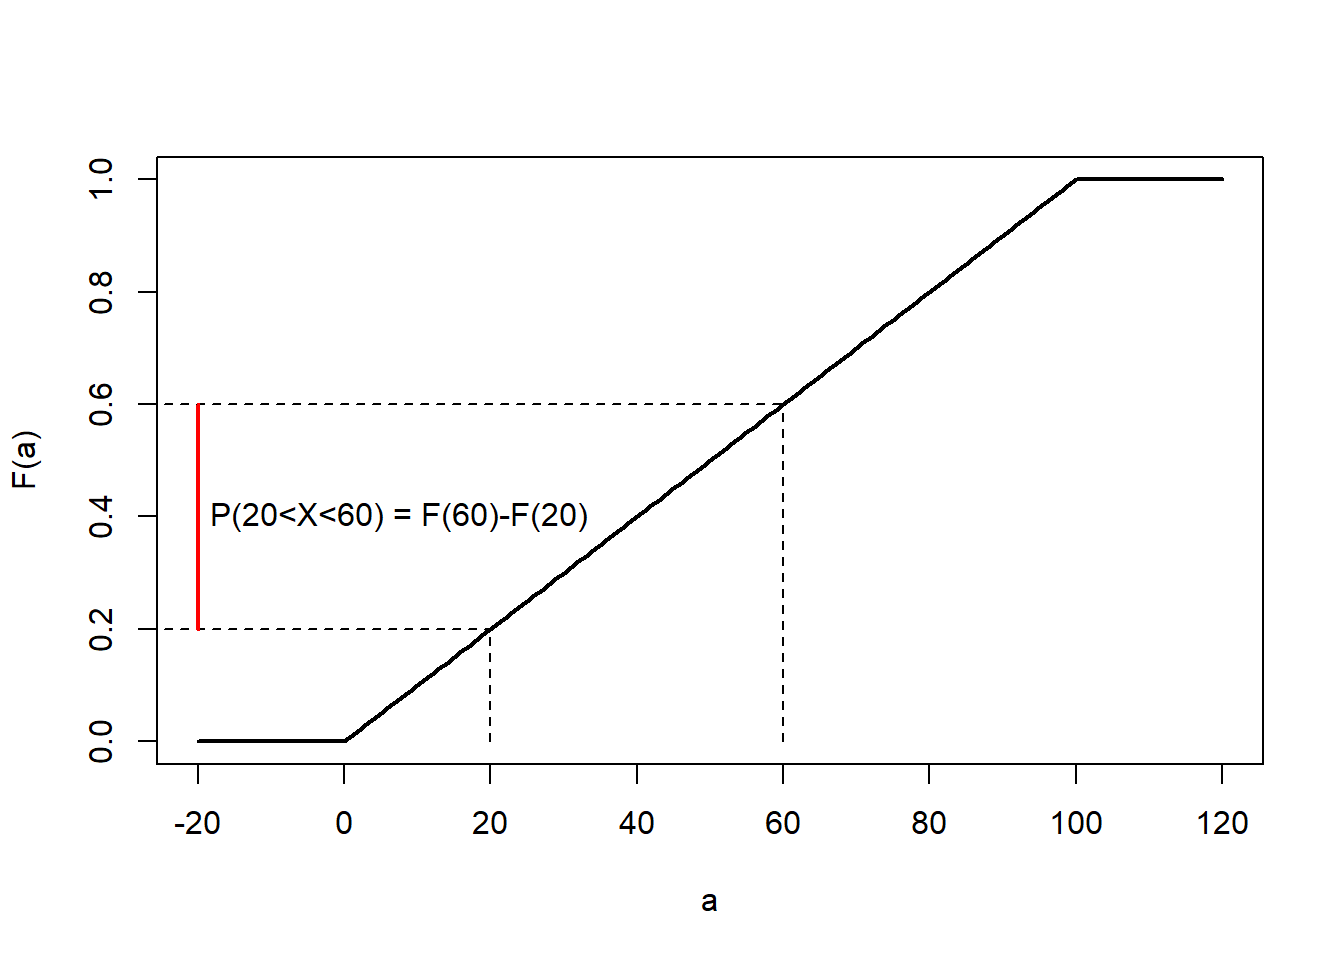
\includegraphics{_main_files/figure-latex/unnamed-chunk-51-1.pdf}

\begin{center}\rule{0.5\linewidth}{0.5pt}\end{center}

\begin{center}\rule{0.5\linewidth}{0.5pt}\end{center}

\hypertarget{distribuciuxf3n-uniforme-dos-paruxe1metros}{%
\section{Distribución uniforme (dos parámetros)}\label{distribuciuxf3n-uniforme-dos-paruxe1metros}}

Presentemos un nuevo modelo de probabilidad uniforme con \textbf{dos parámetros}: los resultados mínimo y máximo.

Si la variable aleatoria toma valores en \(\{a, a+1, ...b\}\), donde \(a\) y \(b\) son números enteros y todos los resultados son igualmente probables, entonces

\[f(x)=\frac{1}{b-a+1}\]

como \(M=b-a+1\).

\begin{itemize}
\tightlist
\item
  Entonces decimos que \(X\) se distribuye uniformemente entre \(a\) y \(b\) y escribimos
\end{itemize}

\[X \rightarrow Unif(a,b)\]

\begin{center}\rule{0.5\linewidth}{0.5pt}\end{center}

\begin{center}\rule{0.5\linewidth}{0.5pt}\end{center}

\hypertarget{distribuciuxf3n-uniforme-dos-paruxe1metros-1}{%
\section{Distribución uniforme (dos parámetros)}\label{distribuciuxf3n-uniforme-dos-paruxe1metros-1}}

\textbf{Ejemplo:}

¿Cuál es la probabilidad de observar a un niño de una edad particular en una escuela primaria (si todas las clases tienen la misma cantidad de niños)?

Del experimento sabemos: \(a=6\) y \(b=11\) entonces

\[X \rightarrow Unif(a=6, b=11)\] eso es

\[f(x)=\frac{1}{6}\] para \(x\in \{6,7,8,9,10,11\}\), y \(0\) en caso contrario

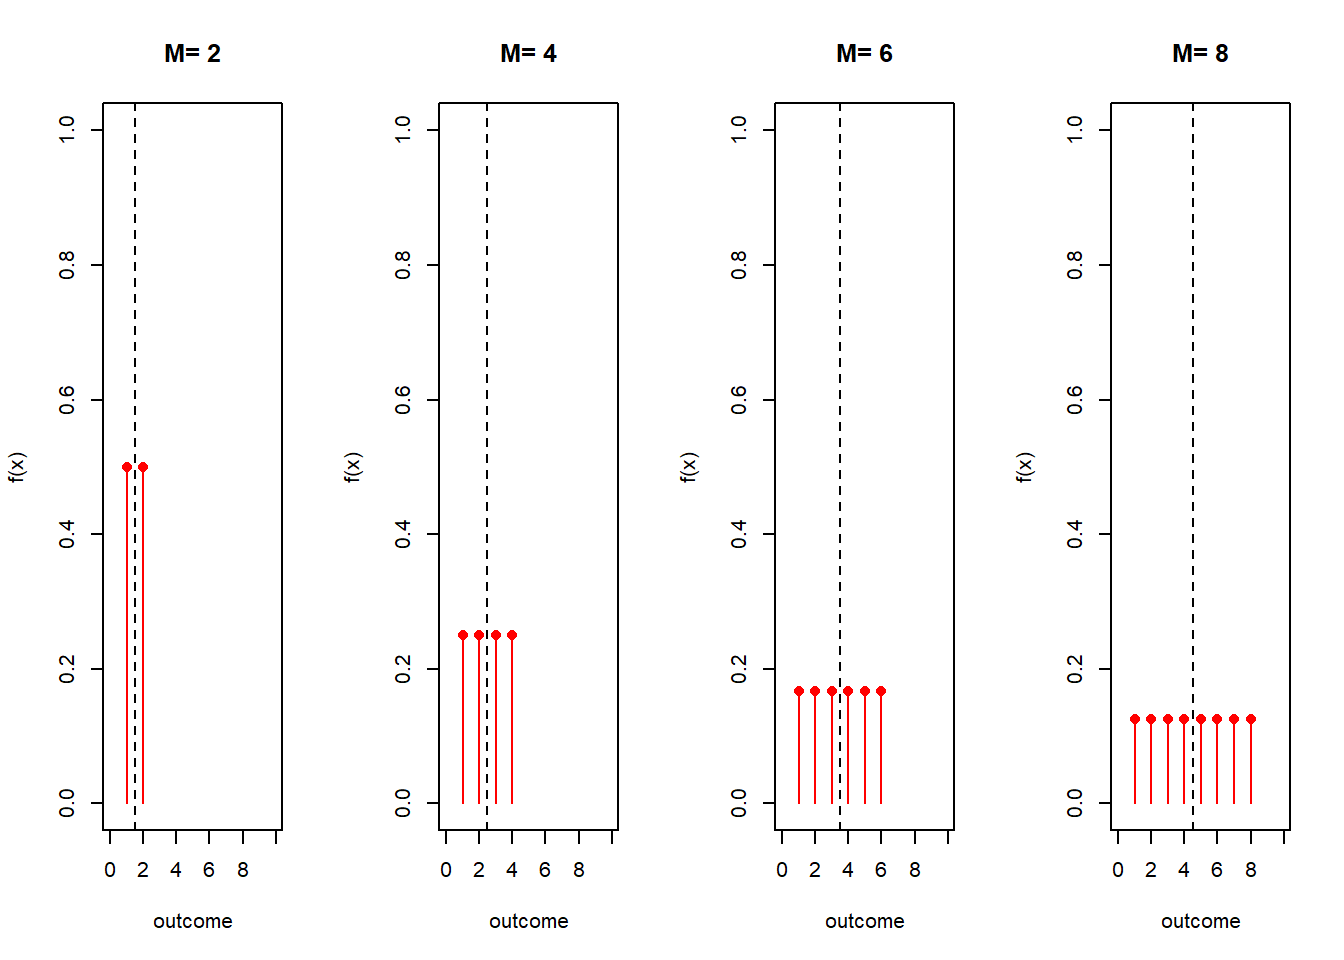
\includegraphics{_main_files/figure-latex/unnamed-chunk-52-1.pdf}

\begin{center}\rule{0.5\linewidth}{0.5pt}\end{center}

\begin{center}\rule{0.5\linewidth}{0.5pt}\end{center}

\hypertarget{distribuciuxf3n-uniforme-1}{%
\section{Distribución uniforme}\label{distribuciuxf3n-uniforme-1}}

El modelo de probabilidad de una variable aleatoria \(X\)

\[f(x)=\frac{1}{b-a+1}\]

para \(x \in \{a, a+1, ...b\}\)

tiene media y varianza:

\begin{itemize}
\item
  \(E(X)= \frac{b+a}{2}\)
\item
  \(V(X)= \frac{(b-a+1)^2-1}{12}\)
\end{itemize}

(Cambiar variables \(X=Y+a-1\), \(y \in \{1,...M\}\))

Podemos especificar \(a\) y \(b\) o \(E(X)\) y \(V(X)\).

En nuestro ejemplo:

\begin{itemize}
\tightlist
\item
  \(E(X)=(11+6)/2=8.5\)
\item
  \(V(X)=(6^2-1)/12=2.916667\)
\end{itemize}

\begin{center}\rule{0.5\linewidth}{0.5pt}\end{center}

\begin{center}\rule{0.5\linewidth}{0.5pt}\end{center}

\hypertarget{distribuciuxf3n-uniforme-dos-paruxe1metros-2}{%
\section{Distribución uniforme (dos parámetros)}\label{distribuciuxf3n-uniforme-dos-paruxe1metros-2}}

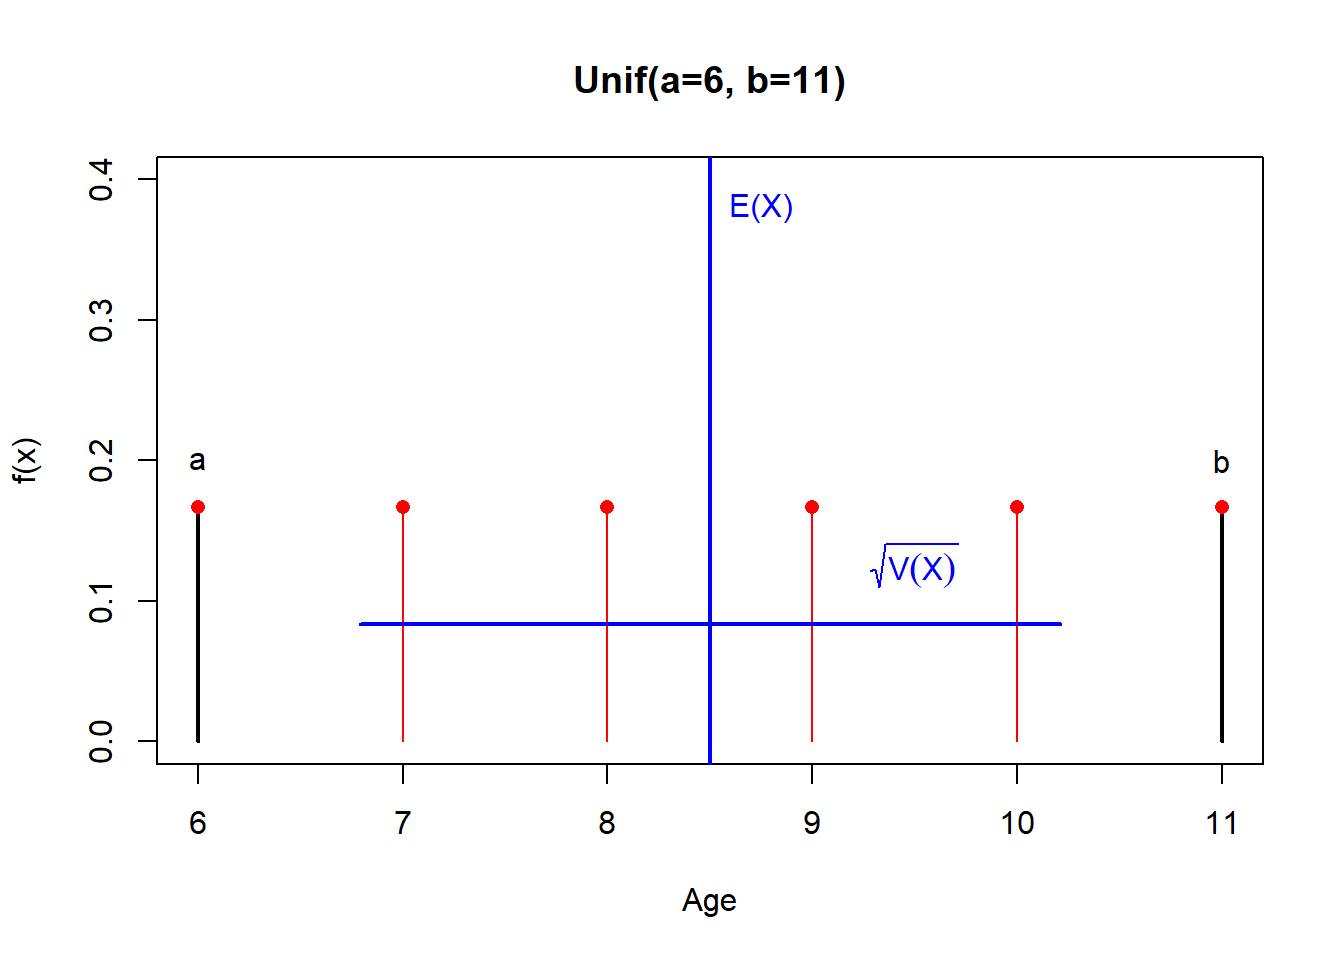
\includegraphics{_main_files/figure-latex/unnamed-chunk-53-1.pdf}

\begin{center}\rule{0.5\linewidth}{0.5pt}\end{center}

\begin{center}\rule{0.5\linewidth}{0.5pt}\end{center}

\hypertarget{paruxe1metros-y-modelos}{%
\section{Parámetros y Modelos}\label{paruxe1metros-y-modelos}}

\begin{itemize}
\item
  Un \textbf{modelo} es una función particular \(f(x)\) que \textbf{describe} nuestro experimento
\item
  Si el modelo es una función \textbf{conocida} que depende de algunos parámetros, al cambiar el valor de los parámetros producimos una \textbf{familia de modelos}
\item
  El conocimiento de \(f(x)\) se reduce al conocimiento del valor de los parámetros
\item
  Idealmente, el modelo y los parámetros son \textbf{interpretables}
\end{itemize}

\emph{Ejemplo:}

\textbf{Modelo}: Los datos de nuestro experimento se producen mediante un proceso aleatorio en el que cada edad tiene la \textbf{misma probabilidad} de ser observada.

\textbf{Parámetros}: \(a\) es la edad mínima, \(E(X)\) es la edad esperada\ldots{} son \textbf{propiedades físicas} del experimento.

\begin{center}\rule{0.5\linewidth}{0.5pt}\end{center}

\begin{center}\rule{0.5\linewidth}{0.5pt}\end{center}

\hypertarget{paruxe1metros-y-modelos-1}{%
\section{Parámetros y Modelos}\label{paruxe1metros-y-modelos-1}}

\textbf{Ejemplo:}

Una \textbf{familia} de modelos obtenidos a partir de distribuciones uniformes de dos parámetros cambiando las \textbf{varianzas} y manteniendo una media constante (\(E(X)=8.5\)). Da como resultado \textbf{cambiar} los resultados \textbf{mínimo} y \textbf{máximo}.

\begin{itemize}
\tightlist
\item
  Nota: solo un modelo tiene sentido para nuestro experimento (solo un modelo puede representar las edades de los niños en una escuela).
\end{itemize}

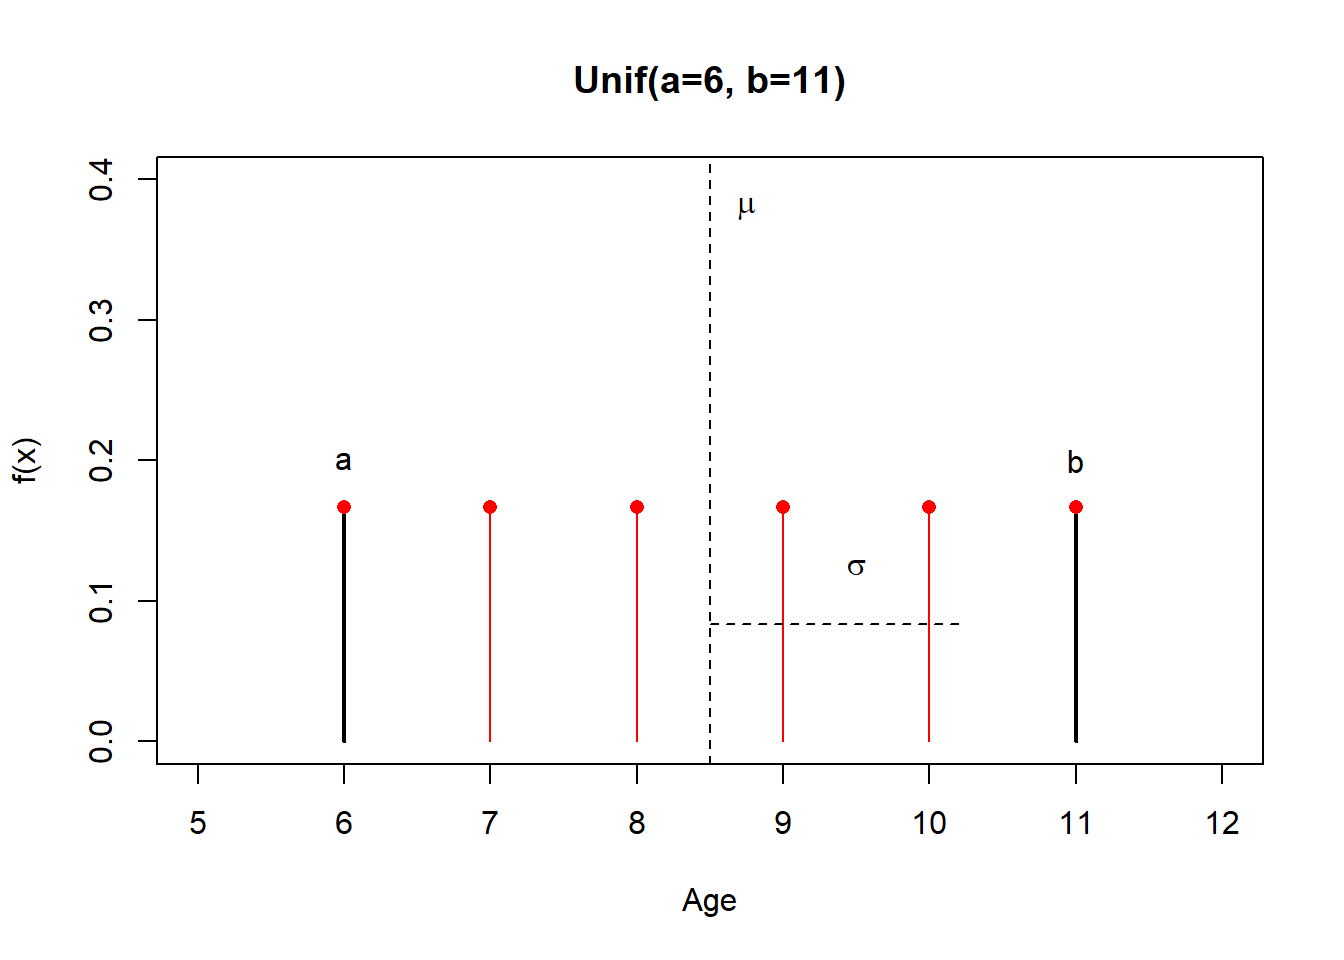
\includegraphics{_main_files/figure-latex/unnamed-chunk-54-1.pdf}

\begin{itemize}
\tightlist
\item
  Podemos pensar en \textbf{familias} que cambian solo en la \textbf{media}, solo el \textbf{mínimo} o solo el \textbf{máximo}
\end{itemize}

\begin{center}\rule{0.5\linewidth}{0.5pt}\end{center}

\begin{center}\rule{0.5\linewidth}{0.5pt}\end{center}

\hypertarget{ensayo-de-bernoulli}{%
\section{Ensayo de Bernoulli}\label{ensayo-de-bernoulli}}

Intentemos avanzar desde el caso de probabilidad igual y supongamos un modelo con dos resultados (\(A\) y \(B\)) que tienen probabilidades \textbf{desiguales}

\textbf{Ejemplos:}

\begin{itemize}
\item
  Anotar el sexo de un paciente que acude a urgencias de un hospital (\(A:masculino\) y \(B:femenino\)).
\item
  Registrar si una máquina fabricada está defectuosa o no (\(A:defectuosa\) y \(B:buena\)).
\item
  Dar en el blanco (\(A:éxito\) y \(B:fracaso\)).
\item
  Transmitiendo un píxel correctamente (\(A:sí\) y \(B:no\)).
\end{itemize}

En estos ejemplos, la probabilidad del resultado \(A\) suele ser \textbf{desconocida}.

\begin{center}\rule{0.5\linewidth}{0.5pt}\end{center}

\begin{center}\rule{0.5\linewidth}{0.5pt}\end{center}

\hypertarget{ensayo-de-bernoulli-1}{%
\section{Ensayo de Bernoulli}\label{ensayo-de-bernoulli-1}}

Introduciremos la probabilidad de un resultado (\(A\)) como el \textbf{parámetro} del modelo:

\begin{itemize}
\tightlist
\item
  resultado A (éxito): tiene probabilidad \(p\) (parámetro)
\item
  resultado B (fracaso): tiene una probabilidad \(1-p\)
\end{itemize}

O podemos escribir la función de masa de probabilidad de \(K\) tomando valores \(\{0, 1\}\) para \(A\) y \(B\)

\[
    f(k)= 
\begin{cases}
    1-p,&  k=0\, (evento\, B)\\
    p,& k=1\, (evento\, A) 
\end{cases}
\]

o más en breve

\[f(k; p)=(1-p)^{1-k} p^k\]
para \(k=(0,1)\)

Solo necesitamos saber \(p\).

\begin{center}\rule{0.5\linewidth}{0.5pt}\end{center}

\begin{center}\rule{0.5\linewidth}{0.5pt}\end{center}

\hypertarget{ensayo-de-bernoulli-2}{%
\section{Ensayo de Bernoulli}\label{ensayo-de-bernoulli-2}}

Una variable de Bernoulli \(K\) con resultados \(\{0, 1\}\) tiene una función de masa de probabilidad

\[f(k; p)=(1-p)^{1-k} p^k\]
Con media y varianza:

\begin{itemize}
\item
  \(E(K)=p\)
\item
  \(V(K)=(1-p)p\)
\end{itemize}

Nota:

\begin{itemize}
\item
  La probabilidad del resultado \(A\) es el parámetro \(p\)
  que es lo mismo que \(f(0)=P(X=0)\).
\item
  Como \(p\) suele ser \textbf{desconocido}, normalmente lo estimamos por la frecuencia relativa (más sobre esto en las secciones de inferencia): \(\hat{p}=f_A=\frac{n_A}{N}\)
\end{itemize}

\begin{center}\rule{0.5\linewidth}{0.5pt}\end{center}

\begin{center}\rule{0.5\linewidth}{0.5pt}\end{center}

\hypertarget{ensayo-de-bernoulli-3}{%
\section{Ensayo de Bernoulli}\label{ensayo-de-bernoulli-3}}

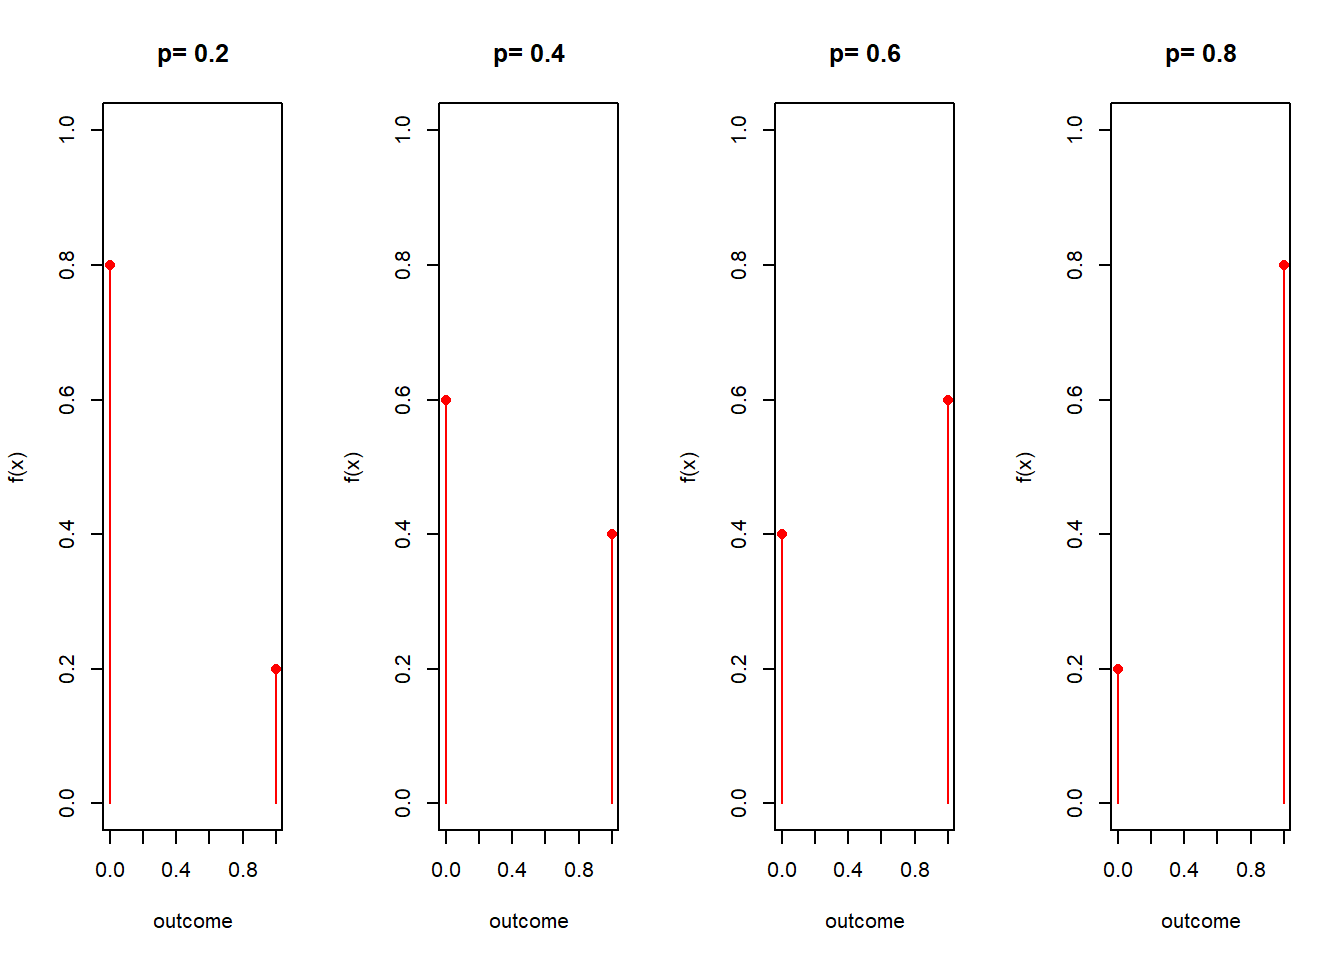
\includegraphics{_main_files/figure-latex/unnamed-chunk-55-1.pdf}

\begin{center}\rule{0.5\linewidth}{0.5pt}\end{center}

\begin{center}\rule{0.5\linewidth}{0.5pt}\end{center}

\hypertarget{distribuciuxf3n-binomial}{%
\section{Distribución binomial}\label{distribuciuxf3n-binomial}}

Cuando estamos interesados \hspace{0pt}\hspace{0pt}en aprender sobre un ensayo de Bernoulli en particular

\begin{itemize}
\item
  Repetimos el ensayo de Bernoulli \(N\) veces y contamos cuantas veces obtuvimos \(A\) (\(n_A\)).
\item
  Definimos una variable aleatoria \(X=n_A\) tomando valores \(x \in {0,1,...N}\)
\end{itemize}

Ahora preguntamos por la probabilidad de observar \(x\) eventos de tipo \(A\) en la repetición de \(n\) ensayos independientes de Bernoulli, cuando la probabilidad de observar \(A\) es \(p\).

\[P(X=x)=f(x)=?\]

\begin{center}\rule{0.5\linewidth}{0.5pt}\end{center}

\begin{center}\rule{0.5\linewidth}{0.5pt}\end{center}

\hypertarget{ejemplos-distribuciuxf3n-binomial}{%
\section{Ejemplos: distribución binomial}\label{ejemplos-distribuciuxf3n-binomial}}

\begin{itemize}
\item
  Anotar el sexo de \(n=10\) pacientes que acuden a urgencias de un hospital. ¿Cuál es la probabilidad de que \(x=6\) los pacientes sean hombres cuando \(p=0,9\)?
\item
  Intentar \(n=5\) veces para dar en el blanco (\(A:éxito\) y \(B:fracaso\)). ¿Cuál es la probabilidad de que alcance el objetivo \(x=5\) veces cuando normalmente lo hago el \(20\%\) de las veces (\(p=0,25\))?
\item
  Transmitiendo \(n=100\) píxeles correctamente (\(A:sí\) y \(B:no\)). ¿Cuál es la probabilidad de que \(x=2\) píxeles sean errores, cuando la probabilidad de error es \(p=0,1\)?
\end{itemize}

\begin{center}\rule{0.5\linewidth}{0.5pt}\end{center}

\begin{center}\rule{0.5\linewidth}{0.5pt}\end{center}

\hypertarget{distribuciuxf3n-binomial-1}{%
\section{Distribución binomial}\label{distribuciuxf3n-binomial-1}}

¿Cuál es la probabilidad de observar \(X=4\) errores al transmitir \(4\) píxeles, si la probabilidad de error es \(p\)?

Considere las variables aleatorias \(4\): \(K_1\), \(K_2\), \(K_3\) y \(K_4\) que registran si se ha cometido un error en el \(1^{o}\), \(2^{o}\), \(3^{r}\) y \(4^{o}\) píxel.

Por lo tanto

\begin{itemize}
\item
  \(k_i\) toma valores \(\{correcto:0; error:1\}\)
\item
  \(X=\sum_{i=1}^4 K_i\) toma valores \(\{0,1,2,3,4\}\)
\end{itemize}

Entonces la probabilidad de observar \(4\) errores es:

\begin{itemize}
\tightlist
\item
  \(P(X=4)=P(1,1,1,1)=p*p*p*p=p^4\) porque \(K_i\) son independientes.
\end{itemize}

La probabilidad de observar \(0\) errores es:

\begin{itemize}
\tightlist
\item
  \(P(X=0)=P(0,0,0,0)=(1-p)(1-p)(1-p)(1-p)=(1-p)^4\)
\end{itemize}

La probabilidad de errores de \(3\) es:

\(P(X=3)=P(0,1,1,1)+P(1,0,1,1)+P(1,1,0,1)+P(1,1,1,0)=4p^3(1-p)^1\)

\begin{center}\rule{0.5\linewidth}{0.5pt}\end{center}

\begin{center}\rule{0.5\linewidth}{0.5pt}\end{center}

\hypertarget{distribuciuxf3n-binomial-2}{%
\section{Distribución binomial}\label{distribuciuxf3n-binomial-2}}

Por lo tanto, la probabilidad de \(x\) errores es

\[
    f(x)=
\begin{cases}
    1*p^0(1-p)^4 & x=0 \\
    4*p^1(1-p)^3,& x=1 \\
    6*p^2(1-p)^2,& x=2 \\
    4*p^3(1-p)^1,& x=3 \\
    1*p^4(1-p)^0 & x=4 \\
\end{cases}
\]

o más en breve

\[f(x)=\binom 4 x p^x(1-p)^{4-x}\]
para \(x=0,1,2,3,4\)

donde \(\binom 4 x\) es el número de posibles resultados (transmisiones de \(4\) píxeles) con \(x\) errores.

\begin{center}\rule{0.5\linewidth}{0.5pt}\end{center}

\begin{center}\rule{0.5\linewidth}{0.5pt}\end{center}

\hypertarget{distribuciuxf3n-binomial-definiciuxf3n}{%
\section{Distribución binomial: Definición}\label{distribuciuxf3n-binomial-definiciuxf3n}}

La función de probabilidad binomial es la función de masa de probabilidad de observar \(x\) resultados de tipo \(A\) en \(n\) ensayos independientes de Bernoulli, donde \(A\) tiene la misma probabilidad \(p\) en cada ensayo.

La función está dada por

\(f(x)=\binom n x p^x(1-p)^{n-x}\), \(x=0,1,...n\)

\(\binom n x= \frac{n!}{x!(n-x)!}\) se denomina \textbf{coeficiente binomial} y da el número de formas en que se pueden obtener \(x\) eventos de tipo \(A\) en un conjunto de \(n\).

Cuando una variable \(X\) tiene una función de probabilidad binomial decimos que se distribuye binomialmente y escribimos

\[X\rightarrow Bin(n,p)\]

donde \(n\) y \(p\) son parámetros.

\begin{center}\rule{0.5\linewidth}{0.5pt}\end{center}

\begin{center}\rule{0.5\linewidth}{0.5pt}\end{center}

\hypertarget{distribuciuxf3n-binomial-media-y-varianza}{%
\section{Distribución binomial: Media y Varianza}\label{distribuciuxf3n-binomial-media-y-varianza}}

La media y la varianza de \(X\rightarrow Bin(n,p)\) son

\begin{itemize}
\item
  \(E(X)=np\)
\item
  \(V(X)=np(1-p)\)
\item
  Dado que \(X\) es la suma de \(n\) variables independientes de Bernoulli
\end{itemize}

\(E(X)=E(\sum_{i=1}^n K_i)=np\)

y

\(V(X)=V(\sum_{i=1}^n K_i)=n(1-p)p\)

Ejemplo:

\begin{itemize}
\item
  El valor esperado para el número de errores en la transmisión de 4 píxeles es \(np=4*0.1=0.4\) cuando la probabilidad de error es \(0.1\).
\item
  La varianza es \(n(1-p)p=0.36\)
\end{itemize}

\textbf{Recuerde}: Podemos especificar los parámetros \(n\) y \(p\), o los parámetros \(E(X)\) y \(V(X)\)

\begin{center}\rule{0.5\linewidth}{0.5pt}\end{center}

\begin{center}\rule{0.5\linewidth}{0.5pt}\end{center}

\hypertarget{ejemplo-1-1}{%
\section{Ejemplo 1}\label{ejemplo-1-1}}

Ahora respondamos:

\begin{itemize}
\tightlist
\item
  ¿Cuál es la probabilidad de observar \(4\) errores al transmitir \(4\) píxeles, si la probabilidad de un error es de \(0.1\)?
\end{itemize}

Dado que estamos repitiendo una prueba de Bernoulli \(n=4\) veces y contando el número de eventos de tipo \(A\) (errores), cuando \(P(A)=p=0.1\) entonces

\[X \rightarrow Bin(n=4, p=0.1)\]
Eso es \[f(x)=\binom 4 x 0.1^x(1-0.1)^{4-x}\]

\begin{center}\rule{0.5\linewidth}{0.5pt}\end{center}

\begin{center}\rule{0.5\linewidth}{0.5pt}\end{center}

\hypertarget{ejemplo-1-2}{%
\section{Ejemplo 1}\label{ejemplo-1-2}}

\begin{itemize}
\tightlist
\item
  Queremos calcular:
\end{itemize}

\(P(X=4)=f(4)=\binom 4 4 0.1^4 0.9^{0}=0.1^4=10^{-4}\)

En R dbinom(4,4,0.1)

\begin{itemize}
\tightlist
\item
  También podemos calcular:
\end{itemize}

\(P(X=2)=\binom 4 2 0.1^2 0.9^2=0.0486\)

En R dbinom(2,4,0.1)

\begin{center}\rule{0.5\linewidth}{0.5pt}\end{center}

\begin{center}\rule{0.5\linewidth}{0.5pt}\end{center}

\hypertarget{ejemplo-2-1}{%
\section{Ejemplo 2}\label{ejemplo-2-1}}

\begin{itemize}
\tightlist
\item
  ¿Cuál es la probabilidad de observar a lo mucho \(8\) votantes del partido de gobierno en una encuesta electoral de tamaño \(10\), si la probabilidad de un voto positivo es de \(0.9\)?
\end{itemize}

Para este caso

\[X \rightarrow Bin(n=10, p=0.9)\]

Eso es \[f(x)=\binom {10} x 0.9^x(0.1)^{4-x}\]

Queremos calcular:
\(P(X\le 8)=F(8)= \sum_{i=1..8} f(x_i)=0.2639011\)

en R pbinom(8,10, 0.9)

\begin{center}\rule{0.5\linewidth}{0.5pt}\end{center}

\begin{center}\rule{0.5\linewidth}{0.5pt}\end{center}

\hypertarget{distribuciuxf3n-binomial-3}{%
\section{Distribución binomial}\label{distribuciuxf3n-binomial-3}}

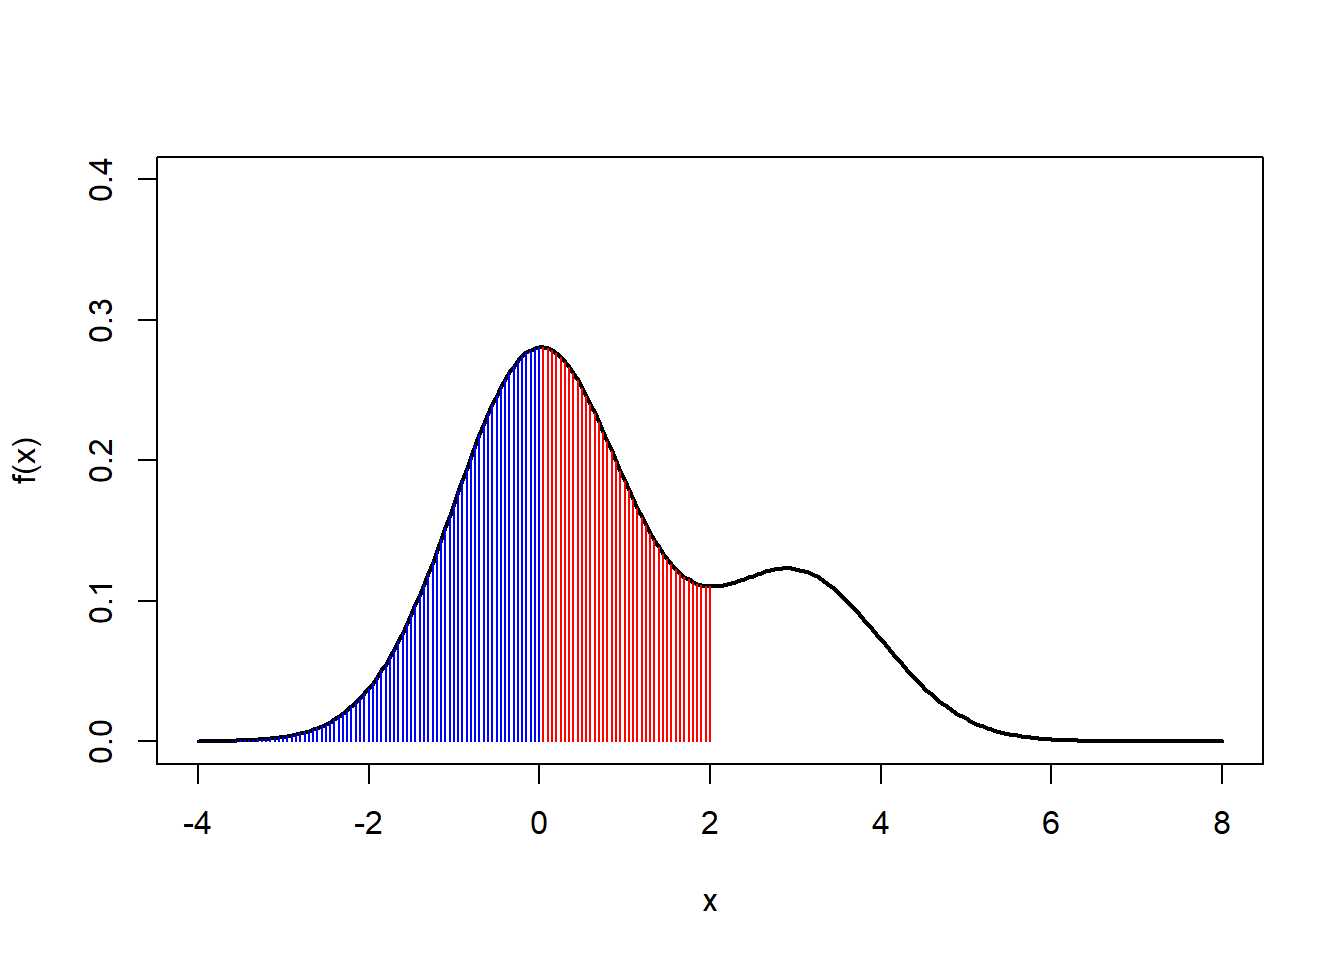
\includegraphics{_main_files/figure-latex/unnamed-chunk-56-1.pdf}

\begin{center}\rule{0.5\linewidth}{0.5pt}\end{center}

\begin{center}\rule{0.5\linewidth}{0.5pt}\end{center}

\hypertarget{distribuciuxf3n-binomial-negativa}{%
\section{Distribución binomial negativa}\label{distribuciuxf3n-binomial-negativa}}

Ahora imaginemos que estamos interesados en contar los píxeles bien transmitidos antes de que ocurra un \textbf{número dado} de errores. Digamos que podemos \textbf{tolerar} \(r\) errores en la transmisión.

\begin{itemize}
\item
  Experimento: Supongamos que realizamos ensayos de Bernoulli hasta que observamos que el resultado \(A\) aparece \(r\) veces.
\item
  Variable aleatoria: Contamos el número de eventos \(B\)
\item
  Ejemplo: ¿Cuál es la probabilidad de observar \(y\) píxeles bien transmitidos (\(B\)) antes de \(r\) errores (\(A\))?
\end{itemize}

\begin{center}\rule{0.5\linewidth}{0.5pt}\end{center}

\begin{center}\rule{0.5\linewidth}{0.5pt}\end{center}

\hypertarget{distribuciuxf3n-binomial-negativa-1}{%
\section{Distribución binomial negativa}\label{distribuciuxf3n-binomial-negativa-1}}

Primero encontremos la probabilidad de una transmisión en particular con \(y\) número de píxeles correctos (\(B\)) y \(r\) número de errores (\(A\)).

\((0,0,1,., 0,1,...0,1)\) (hay \(y\) ceros y \(r\) unos)

Observamos \(y\) píxeles correctos en un total de \(y + r\) intentos.

Por lo tanto

\begin{itemize}
\tightlist
\item
  \(P(0,0,1,., 0,1,...0,1)=(1-p)^yp^r\) (Recuerda: \(p\) es la probabilidad de error)
\end{itemize}

¿Cuántas transmisiones pueden tener \(y\) píxeles correctos antes de \(r\) errores?

Nota:

\begin{itemize}
\item
  El último bit es fijo (marca el final de la transmisión)
\item
  El número total de transmisiones con \(y\) número de píxeles correctos (\(B\)) que podemos obtener en \(y + r-1\) intentos es: \(\binom {y + r-1} y\)
\end{itemize}

\begin{center}\rule{0.5\linewidth}{0.5pt}\end{center}

\begin{center}\rule{0.5\linewidth}{0.5pt}\end{center}

\hypertarget{distribuciuxf3n-binomial-negativa-2}{%
\section{Distribución binomial negativa}\label{distribuciuxf3n-binomial-negativa-2}}

Por lo tanto, la probabilidad de observar \(y\) eventos de tipo \(B\) antes de \(r\) eventos de tipo \(A\) (con probabilidad \(p\)) es

\[P(Y=y)=f(y)=\binom {y+r-1} y (1-p)^yp^r\]

para \(y=0,1,...\)

Entonces decimos que \(Y\) sigue una distribución binomial negativa y escribimos

\[Y\rightarrow NB(r,p)\]

donde \(r\) y \(p\) son parámetros que representan la tolerancia y la probabilidad de un solo error.

\begin{center}\rule{0.5\linewidth}{0.5pt}\end{center}

\begin{center}\rule{0.5\linewidth}{0.5pt}\end{center}

\hypertarget{media-y-varianza-2}{%
\section{Media y Varianza}\label{media-y-varianza-2}}

Una variable aleatoria con \(Y\rightarrow NB(r,p)\) tiene

\begin{itemize}
\item
  media: \(E(Y)= r\frac{1-p}{p}\)
\item
  varianza: \(V(Y)= r\frac{1-p}{p^2}\)
\end{itemize}

\begin{center}\rule{0.5\linewidth}{0.5pt}\end{center}

\begin{center}\rule{0.5\linewidth}{0.5pt}\end{center}

\hypertarget{distribuciuxf3n-geomuxe9trica}{%
\section{Distribución geométrica}\label{distribuciuxf3n-geomuxe9trica}}

Llamamos \textbf{distribución geométrica} a la distribución binomial negativa con \(r=1\)

La probabilidad de observar \(B\) eventos antes de observar el \textbf{primer} evento de tipo \(A\) es

\[P(Y=y)=f(y)= (1-p)^yp\]

\[Y\rightarrow Geom(p)\]
con media

\begin{itemize}
\item
  media: \(E(Y)= \frac{1-p}{p}\)
\item
  varianza: \(V(Y)= \frac{1-p}{p^2}\)
\end{itemize}

\begin{center}\rule{0.5\linewidth}{0.5pt}\end{center}

\begin{center}\rule{0.5\linewidth}{0.5pt}\end{center}

\hypertarget{ejemplo-9}{%
\section{Ejemplo}\label{ejemplo-9}}

\begin{itemize}
\item
  Un sitio web tiene tres servidores.
\item
  Un servidor opera a la vez y solo cuando falla una solicitud se utiliza otro servidor.
\item
  Si se sabe que la probabilidad de que falle una solicitud es \(p=0.0005\), entonces
\item
  ¿Cuál es el número esperado de solicitudes exitosas antes de que los tres servidores fallen?
\end{itemize}

\begin{center}\rule{0.5\linewidth}{0.5pt}\end{center}

\begin{center}\rule{0.5\linewidth}{0.5pt}\end{center}

\hypertarget{ejemplo-10}{%
\section{Ejemplo}\label{ejemplo-10}}

Ya que estamos repitiendo un ensayo de Bernoulli hasta que se observan \(r=3\) eventos de tipo \(A\) (cada uno con \(P(A)=p=0.0005\)) y estamos contando el número de eventos de tipo \(B\) (errores) entonces

\[Y \rightarrow NB(r=3, p=0.0005)\]

Por lo tanto, el número esperado de solicitudes antes de que el sistema falle es:

\(E(Y)=r\frac{1-p}{p}=3\frac{1-0.0005}{0.0005}=5997\)

\begin{itemize}
\tightlist
\item
  Tenga en cuenta que para enviar este número de solicitures hemos enviado un total de \(6000=5997+3\)
\end{itemize}

\begin{center}\rule{0.5\linewidth}{0.5pt}\end{center}

\begin{center}\rule{0.5\linewidth}{0.5pt}\end{center}

\hypertarget{ejemplo-11}{%
\section{Ejemplo}\label{ejemplo-11}}

¿Cuál es la probabilidad de tratar con éxito como máximo \(5\) solicitudes antes de que el sistema falle?

Recuerde la función de distribución: \(F(y)=P(Y\leq 5)\)

\(F(5)=P(Y\leq 5)=\Sigma_{y=0}^5 f(y)\)

\(=\sum_{y=0}^5\binom {y+2} y 0.9995^y 0.0005^r\)

\(=\binom{2} 0 0.9995^0 0.0005^3 +\binom{3} 1 0.9995^1 0.0005^3\)

\(+\binom{4} 2 0.9995^2 0.0005^3 +\binom{5} 3 0.9995^3 0.0005^3\)

\(+\binom {6} 4 0.9995^4 0.0005^3 +\binom {7} 5 0.9995^5 0.0005^3\)

\(= 6.9\times 10^{-9}\)

En R pnbinom(5,3,0.0005)

\begin{center}\rule{0.5\linewidth}{0.5pt}\end{center}

\begin{center}\rule{0.5\linewidth}{0.5pt}\end{center}

\hypertarget{ejemplos}{%
\section{Ejemplos}\label{ejemplos}}

Con la función de probabilidad binomial negativa:

\[f(y)=\binom {y+r-1} y (1-p)^yp^r\]

Ahora podemos responder preguntas como:

\begin{itemize}
\tightlist
\item
  ¿Cuál es la probabilidad de observar \(10\) píxeles correctos antes de \(2\) errores, si la probabilidad de error es \(0.1\)?
\end{itemize}

\(f(10; r=2, p=0.1)=0.03835463\)

en R dnbinom(10, 2, 0.1)

\begin{itemize}
\tightlist
\item
  ¿Cuál es la probabilidad de que entren \(2\) chicas antes que \(4\) chicos si la probabilidad de que entre una chica es de \(0.5\)?
\end{itemize}

\(f(2; r=4, p=0.5)=0.15625\)

en R dnbinom(2, 4, 0.5)

\begin{center}\rule{0.5\linewidth}{0.5pt}\end{center}

\begin{center}\rule{0.5\linewidth}{0.5pt}\end{center}

\hypertarget{distribuciuxf3n-binomial-negativa-3}{%
\section{Distribución binomial negativa}\label{distribuciuxf3n-binomial-negativa-3}}

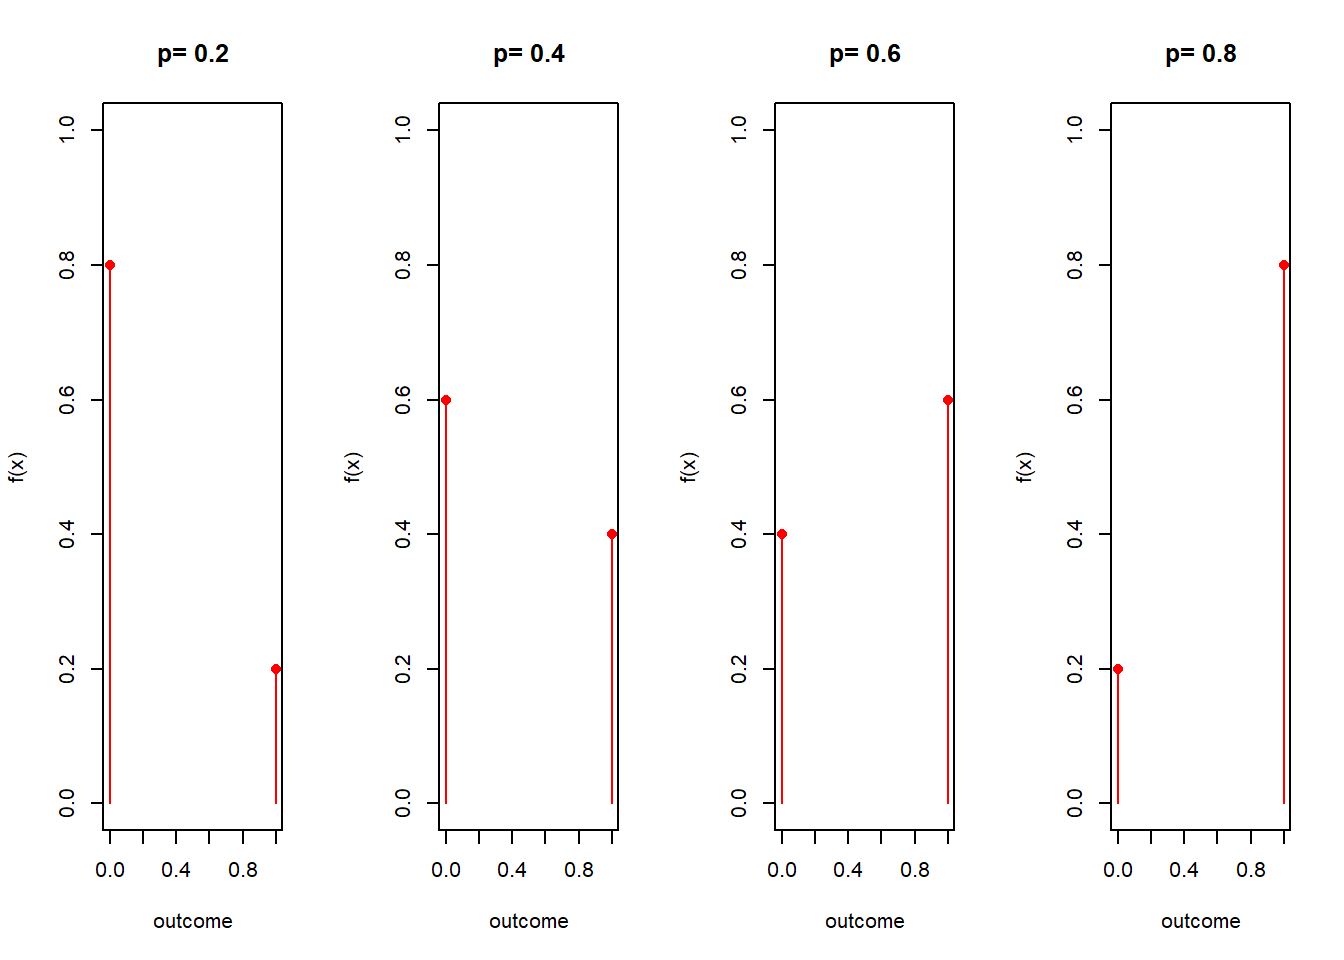
\includegraphics{_main_files/figure-latex/unnamed-chunk-57-1.pdf}

\begin{center}\rule{0.5\linewidth}{0.5pt}\end{center}

\begin{center}\rule{0.5\linewidth}{0.5pt}\end{center}

\hypertarget{distribuciuxf3n-hipergeomuxe9trica}{%
\section{Distribución hipergeométrica}\label{distribuciuxf3n-hipergeomuxe9trica}}

La probabilidad de obtener \(x\) casos de hepatitis C en una muestra de \(n\) extraída de una población de \(N\) donde \(K\) tiene hepatitis C es

\(P(X=x)=P(one\,sample) \times (Number\, of\, ways\, of\, obtaining\, x)\)

\[=\frac{1}{\binom N n}\binom K x \binom {N-K} {n-x}\]

donde \(k \in \{\max(0, n+K-N), ... \min(K, n) \}\)

\[X \rightarrow Hypergeometric(N,K,n)\]

\begin{center}\rule{0.5\linewidth}{0.5pt}\end{center}

\begin{center}\rule{0.5\linewidth}{0.5pt}\end{center}

\hypertarget{distribuciuxf3n-hipergeomuxe9trica-1}{%
\section{Distribución hipergeométrica}\label{distribuciuxf3n-hipergeomuxe9trica-1}}

Una variable hipergeométrica tiene

\begin{itemize}
\item
  media: \(E (X) = n \frac{K}{N} = np_0\)
\item
  varianza: \(V(X) = np_0(1-p_0)\frac{N-n}{N-1}\)
\end{itemize}

cuando \(p_0=\frac{K}{N}\) es la proporción de hepatitis C en una población de tamaño \(N\).

\begin{center}\rule{0.5\linewidth}{0.5pt}\end{center}

\begin{center}\rule{0.5\linewidth}{0.5pt}\end{center}

\hypertarget{distribuciuxf3n-hipergeomuxe9trica-2}{%
\section{Distribución hipergeométrica}\label{distribuciuxf3n-hipergeomuxe9trica-2}}

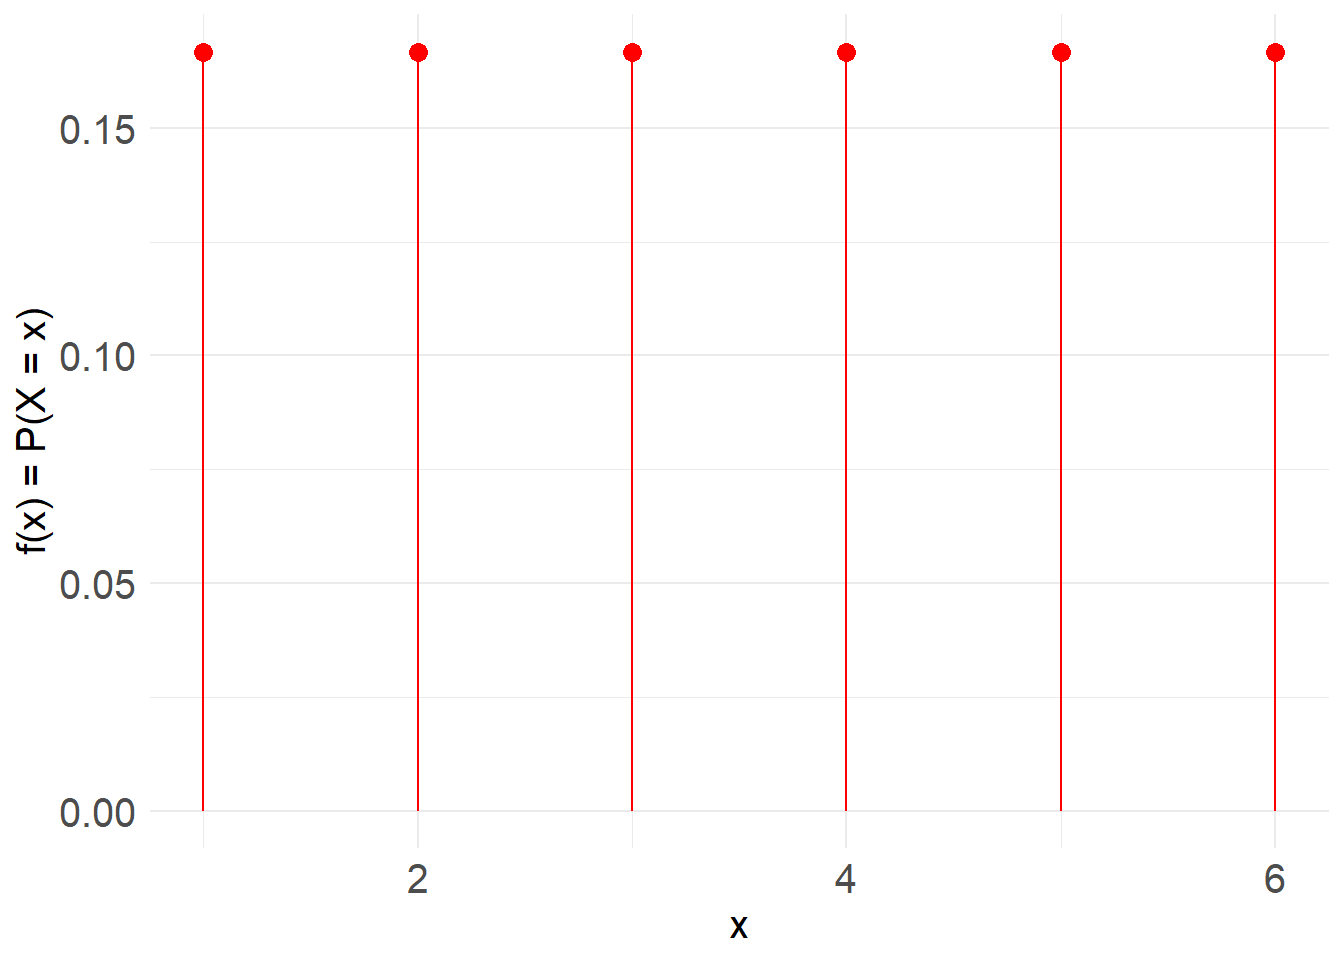
\includegraphics{_main_files/figure-latex/unnamed-chunk-58-1.pdf}

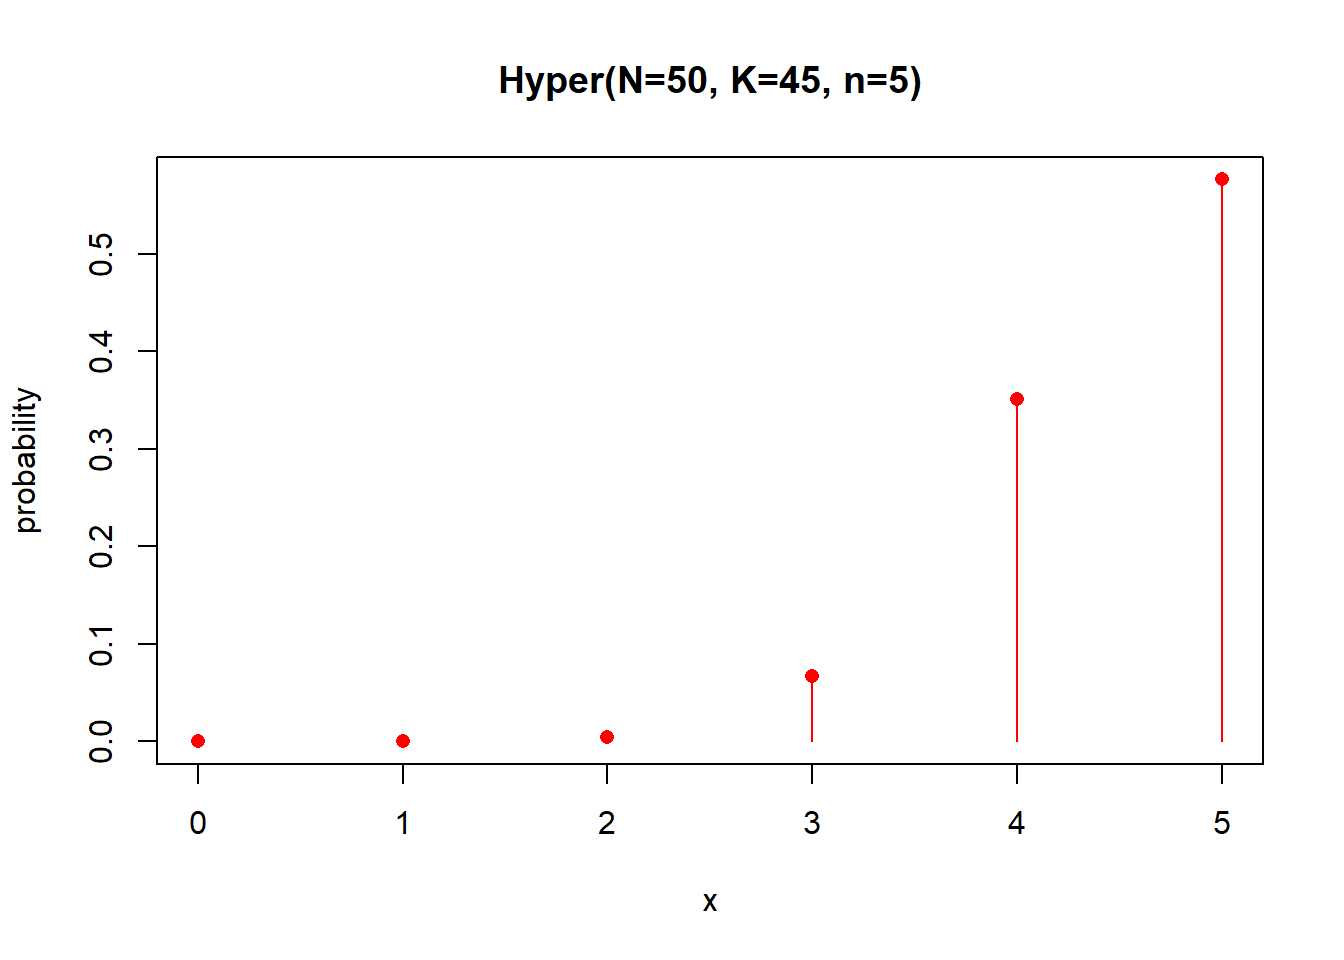
\includegraphics{_main_files/figure-latex/unnamed-chunk-59-1.pdf}

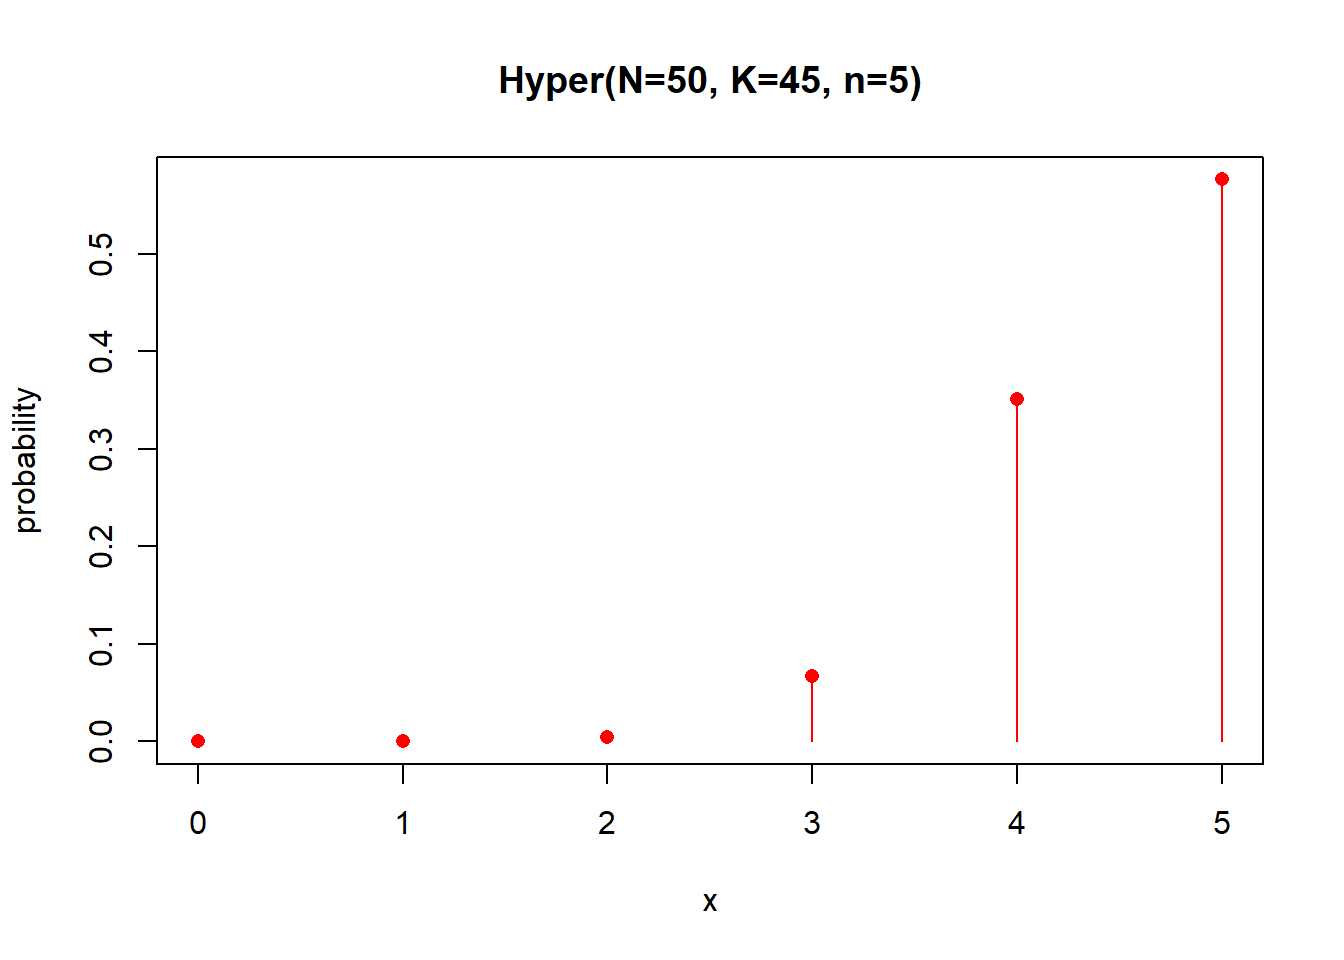
\includegraphics{_main_files/figure-latex/unnamed-chunk-60-1.pdf}

\hypertarget{modelos-de-poisson-y-exponencial}{%
\chapter{Modelos de Poisson y Exponencial}\label{modelos-de-poisson-y-exponencial}}

\hypertarget{objetivo-7}{%
\section{Objetivo}\label{objetivo-7}}

Modelo de probabilidad discreta:

\begin{itemize}
\tightlist
\item
  Poisson
\end{itemize}

Modelo de probabilidad continua:

\begin{itemize}
\tightlist
\item
  Exponencial
\end{itemize}

\begin{center}\rule{0.5\linewidth}{0.5pt}\end{center}

\begin{center}\rule{0.5\linewidth}{0.5pt}\end{center}

\hypertarget{modelos-de-probabilidad-discreta}{%
\section{Modelos de probabilidad discreta}\label{modelos-de-probabilidad-discreta}}

Estamos construyendo modelos más complejos a partir de modelos simples:

\textbf{Uniforme}: interpretación clásica de la probabilidad
\(\downarrow\)
\textbf{Bernoulli}: Introducción de un \textbf{parámetro} \(p\) (familia de modelos)
\(\downarrow\)
\textbf{Binomial}: \textbf{Repetición} de un experimento aleatorio (\(n\)-veces ensayos de Bernoulli)
\(\downarrow\)
\textbf{Poisson}: Repetición de un experimento aleatorio dentro de un intervalo continuo, \textbf{sin control} sobre cuándo/dónde ocurre la ensayo de Bernouilli.

\begin{center}\rule{0.5\linewidth}{0.5pt}\end{center}

\begin{center}\rule{0.5\linewidth}{0.5pt}\end{center}

\hypertarget{contando-eventos}{%
\section{Contando eventos}\label{contando-eventos}}

Imagine que estamos observando eventos que \textbf{dependen} de \textbf{intervalos} de tiempo o distancia.

\begin{itemize}
\tightlist
\item
  coches que llegan a un semáforo
\item
  mensajes en el teléfono móvil
\item
  impurezas que ocurren al azar en un alambre de cobre
\end{itemize}

Supongamos que los eventos son resultados de ensayos de Bernoulli \textbf{independientes}, cada uno de los cuales aparece aleatoriamente en un intervalo continuo, y queremos \textbf{contarlos}.

\begin{center}\rule{0.5\linewidth}{0.5pt}\end{center}

\begin{center}\rule{0.5\linewidth}{0.5pt}\end{center}

\hypertarget{contando-eventos-1}{%
\section{Contando eventos}\label{contando-eventos-1}}

¿Cuál es la probabilidad de observar \(X\) eventos en una unidad de intervalo (tiempo o distancia)?

Imagine que algunas impurezas en un alambre de cobre se depositan al azar a lo largo de un alambre

\begin{itemize}
\tightlist
\item
  en cada centímetro, contamos un promedio de \(\lambda=10/cm\).
\item
  dividimos el centímetro en micrómetros (\(0.0001cm\))
\end{itemize}

\begin{center}\rule{0.5\linewidth}{0.5pt}\end{center}

\begin{center}\rule{0.5\linewidth}{0.5pt}\end{center}

\hypertarget{distribuciuxf3n-de-poisson}{%
\section{Distribución de Poisson}\label{distribuciuxf3n-de-poisson}}

Los micrómetros son lo suficientemente pequeños tal que

\begin{itemize}
\tightlist
\item
  hay o no hay una impureza en cada micrómetro
\item
  cada micrómetro puede considerarse un \textbf{ensayo de Bernoulli}
\end{itemize}

\begin{center}\rule{0.5\linewidth}{0.5pt}\end{center}

\begin{center}\rule{0.5\linewidth}{0.5pt}\end{center}

\hypertarget{distribuciuxf3n-de-poisson-1}{%
\section{Distribución de Poisson}\label{distribuciuxf3n-de-poisson-1}}

La probabilidad de observar \(X\) impurezas en \(n=10,000\mu\) (1cm) sigue aproximadamente una distribución binomial

\(P(X=x)=\binom n x p^x(1-p)^{n-x}\)

donde \(p\) es la probabilidad de encontrar una impureza en un micrómetro.

Recuerdemos que
\(E(X)=np\)
entonces para \(\lambda=np\) (número promedio de impurezas por 1 cm), podemos escribir

\[P(X=x)=\binom n x \big(\frac{\lambda}{n}\big)^x(1-\frac{\lambda}{n})^{n-x}\]

\begin{itemize}
\tightlist
\item
  \textbf{Podría} todavía haber dos impurezas en un micrómetro, por lo que debemos aumentar la partición del cable y \(n \rightarrow \infty\).
\end{itemize}

Entonces en el límite:

\[P(X=x)= \frac{e^{-\lambda}\lambda^x}{x!}\]

Donde \(\lambda\) es constante porque es la densidad de impurezas por centímetro, una \textbf{propiedad física} del sistema.

\begin{center}\rule{0.5\linewidth}{0.5pt}\end{center}

\begin{center}\rule{0.5\linewidth}{0.5pt}\end{center}

\hypertarget{distribuciuxf3n-de-poisson-detalles-de-la-derivaciuxf3n}{%
\section{Distribución de Poisson: detalles de la derivación}\label{distribuciuxf3n-de-poisson-detalles-de-la-derivaciuxf3n}}

Para \(P(X=x)=\binom n x \big(\frac{\lambda}{n}\big)^x(1-\frac{\lambda}{n})^{n-x}\)

en el límite (\(n \rightarrow \infty\))

\begin{itemize}
\tightlist
\item
  \(\frac{1}{n^x}\binom n x =\frac{1}{n^x}\frac{n!}{x! (n-x)!}=\frac{(n-x)!(n-x+1)...(n-1)n}{n^x x! (n-x)!}=\frac{n(n-1)..(n-x+1)}{n^x x!} \rightarrow \frac{1}{x!}\)
\item
  \((1-\frac{\lambda}{n})^{n} \rightarrow e^{-\lambda}\) (definición de exponencial)
\item
  \((1-\frac{\lambda}{n})^{-x} \rightarrow 1\)
\end{itemize}

Por lo tanto
\(P(X=x)= \frac{e^{-\lambda}\lambda^x}{x!}\)

\begin{center}\rule{0.5\linewidth}{0.5pt}\end{center}

\begin{center}\rule{0.5\linewidth}{0.5pt}\end{center}

\hypertarget{distribuciuxf3n-de-poisson-2}{%
\section{Distribución de Poisson}\label{distribuciuxf3n-de-poisson-2}}

\textbf{Definición}

Dado

\begin{itemize}
\tightlist
\item
  un intervalo en los números reales
\item
  los eventos ocurren al azar en el intervalo
\item
  se conoce el número medio de conteos en el intervalo (\(\lambda\))
\item
  se puede encontrar una pequeña partición regular del intervalo tal que cada uno de ellos pueda considerarse un ensayo de Bernoulli
\end{itemize}

Entonces \ldots{}

\begin{center}\rule{0.5\linewidth}{0.5pt}\end{center}

\begin{center}\rule{0.5\linewidth}{0.5pt}\end{center}

\hypertarget{distribuciuxf3n-de-poisson-3}{%
\section{Distribución de Poisson}\label{distribuciuxf3n-de-poisson-3}}

\textbf{Definición}

La variable aleatoria \(X\) que cuenta eventos a lo largo del intervalo es una variable \textbf{Poisson} con función de masa de probabilidad
\[f(x)= \frac{e^{-\lambda}\lambda^x}{x!}, \lambda>0\]

\textbf{Propiedades:}

\begin{itemize}
\tightlist
\item
  media \(E(X)= \lambda\)
\item
  varianza \(V(X)= \lambda\)
\end{itemize}

\begin{center}\rule{0.5\linewidth}{0.5pt}\end{center}

\begin{center}\rule{0.5\linewidth}{0.5pt}\end{center}

\hypertarget{distribuciuxf3n-de-poisson-4}{%
\section{Distribución de Poisson}\label{distribuciuxf3n-de-poisson-4}}

Con la función de probabilidad de Poisson:

\[f(x)= \frac{e^{-\lambda}\lambda^x}{x!}\] para \(x \in \{0, 1, ...\}\)

Podemos responder preguntas como:

\begin{itemize}
\tightlist
\item
  ¿Cuál es la probabilidad de recibir 4 correos electrónicos en una hora, cuando el promedio de correos electrónicos en una horas es de \(1\)?
\end{itemize}

\(f(4; \lambda=1)= 0.18\)

in R dpois(2,1)

\begin{itemize}
\tightlist
\item
  ¿Cuál es la probabilidad de contar al menos \(10\) coches que llegan a un peaje en un minuto, cuando el promedio de autos que llegan a un peaje en un minuto es de \(5\);
  \(P(X \leq 10)=F(10; \lambda=5)=0.98\)?
\end{itemize}

in R ppois(10,5)

\begin{center}\rule{0.5\linewidth}{0.5pt}\end{center}

\begin{center}\rule{0.5\linewidth}{0.5pt}\end{center}

\hypertarget{distribuciuxf3n-de-poisson-5}{%
\section{Distribución de Poisson}\label{distribuciuxf3n-de-poisson-5}}

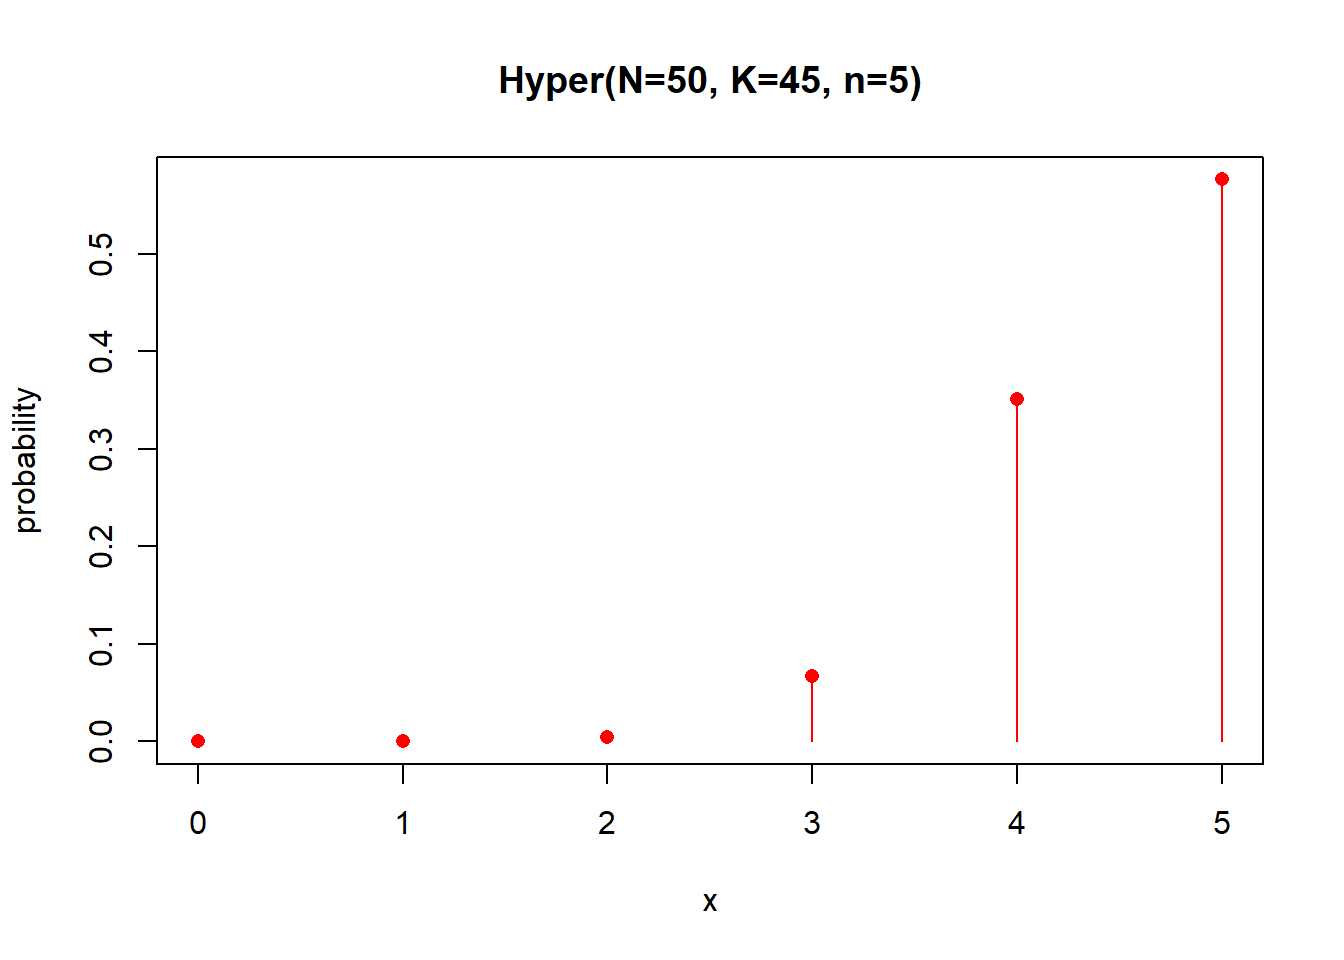
\includegraphics{_main_files/figure-latex/unnamed-chunk-61-1.pdf}

\begin{center}\rule{0.5\linewidth}{0.5pt}\end{center}

\begin{center}\rule{0.5\linewidth}{0.5pt}\end{center}

\hypertarget{modelos-de-probabilidad-continua}{%
\section{Modelos de probabilidad continua}\label{modelos-de-probabilidad-continua}}

Los modelos de probabilidad continua son funciones de densidad de probabilidad \(f(x)\) de variables aleatorias continuas que \textbf{creemos} describen experimentos aleatorios reales.

Definición:

Positiva:

\begin{itemize}
\tightlist
\item
  \(f(x) \geq 0\)
\end{itemize}

\emph{Permite calcular probabilidades usando el área bajo la curva:}

\begin{itemize}
\tightlist
\item
  \(P(a\leq X \leq b)=\int_{a}^{b} f(x) dx\)
\end{itemize}

La probabilidad de observar algún valor es \(1\):

\begin{itemize}
\tightlist
\item
  \(\int_{-\infty}^{\infty} f(x) dx = 1\)
\end{itemize}

\begin{center}\rule{0.5\linewidth}{0.5pt}\end{center}

\begin{center}\rule{0.5\linewidth}{0.5pt}\end{center}

\hypertarget{densidad-exponencial}{%
\section{Densidad exponencial}\label{densidad-exponencial}}

Volvamos a la probabilidad de Poisson para el número de eventos (\(k\)) en un intervalo

\[f(k)=\frac{e^{-\lambda}\lambda^k}{k!}, \lambda>0\]

\begin{itemize}
\item
  Consideremos ahora solo el primer evento (duración/tiempo)
\item
  la distancia/tiempo que debemos esperar hasta el primer evento es una variable aleatoria \textbf{continua}.
\end{itemize}

Podemos preguntar por la probabilidad de que el primer evento esté a la distancia \(X\).

\begin{center}\rule{0.5\linewidth}{0.5pt}\end{center}

\begin{center}\rule{0.5\linewidth}{0.5pt}\end{center}

\hypertarget{densidad-exponencial-1}{%
\section{Densidad exponencial}\label{densidad-exponencial-1}}

La probabilidad de no observar ningún evento \textbf{si} un intervalo tiene unidad \(x\) es

\[f(0|x)=\frac{e^{-x\lambda}x\lambda^0}{0!}\]

o

\[f(0|x)=e^{-x\lambda}\]

Podemos tratar esto como la probabilidad condicional de \(0\) eventos en una distancia \(x\): \(f(K=0|X=x)\) y aplicar el teorema de Bayes para invertirlo:

\[f(x|0)=C f(0|x)=C e^{-x\lambda}\]

Entonces podemos calcular la \textbf{probabilidad de observar una distancia} \(x\) con \(0\) eventos (esta es la distancia hasta el primer evento, o la distancia entre dos eventos).

\begin{center}\rule{0.5\linewidth}{0.5pt}\end{center}

\begin{center}\rule{0.5\linewidth}{0.5pt}\end{center}

\hypertarget{densidad-exponencial-2}{%
\section{Densidad exponencial}\label{densidad-exponencial-2}}

En un proceso de Poisson con parámetro \(\lambda\) la probabilidad de esperar una distancia/tiempo \(X\) hasta el primer evento tiene una \textbf{densidad de probabilidad}

\[f(x)= C e^{-x\lambda}\]

\begin{itemize}
\item
  \(C\) es una constante que asegura: \(\int_{-\infty}^{\infty} f(x) dx =1\)
\item
  por integración \(C=\lambda\)
\end{itemize}

Por lo tanto

\[f(x)=\lambda e^{-\lambda x}\]

\begin{center}\rule{0.5\linewidth}{0.5pt}\end{center}

\begin{center}\rule{0.5\linewidth}{0.5pt}\end{center}

\hypertarget{densidad-exponencial-3}{%
\section{Densidad exponencial}\label{densidad-exponencial-3}}

Una variable aleatoria exponencial \(X\) tiene una densidad de probabilidad

\[f(x)=\lambda e^{-\lambda x}, x\geq 0\]

\textbf{Propiedades:}

\begin{itemize}
\tightlist
\item
  Media: \(E(X)=\frac{1}{\lambda}\)
\item
  Varianza: \(V(Y)=\frac{1}{\lambda^2}\)
\end{itemize}

Donde \(\lambda\) es su único parámetro, conocido como \textbf{tasa de decaimiento}.

\textbf{Nota:} El modelo exponencial es un modelo general. Puede describir el tiempo/duración hasta la primera cuenta en un proceso de Poisson del tamaño de un huevo hecho por un taladro.

\begin{center}\rule{0.5\linewidth}{0.5pt}\end{center}

\begin{center}\rule{0.5\linewidth}{0.5pt}\end{center}

\hypertarget{densidad-exponencial-4}{%
\section{Densidad exponencial}\label{densidad-exponencial-4}}

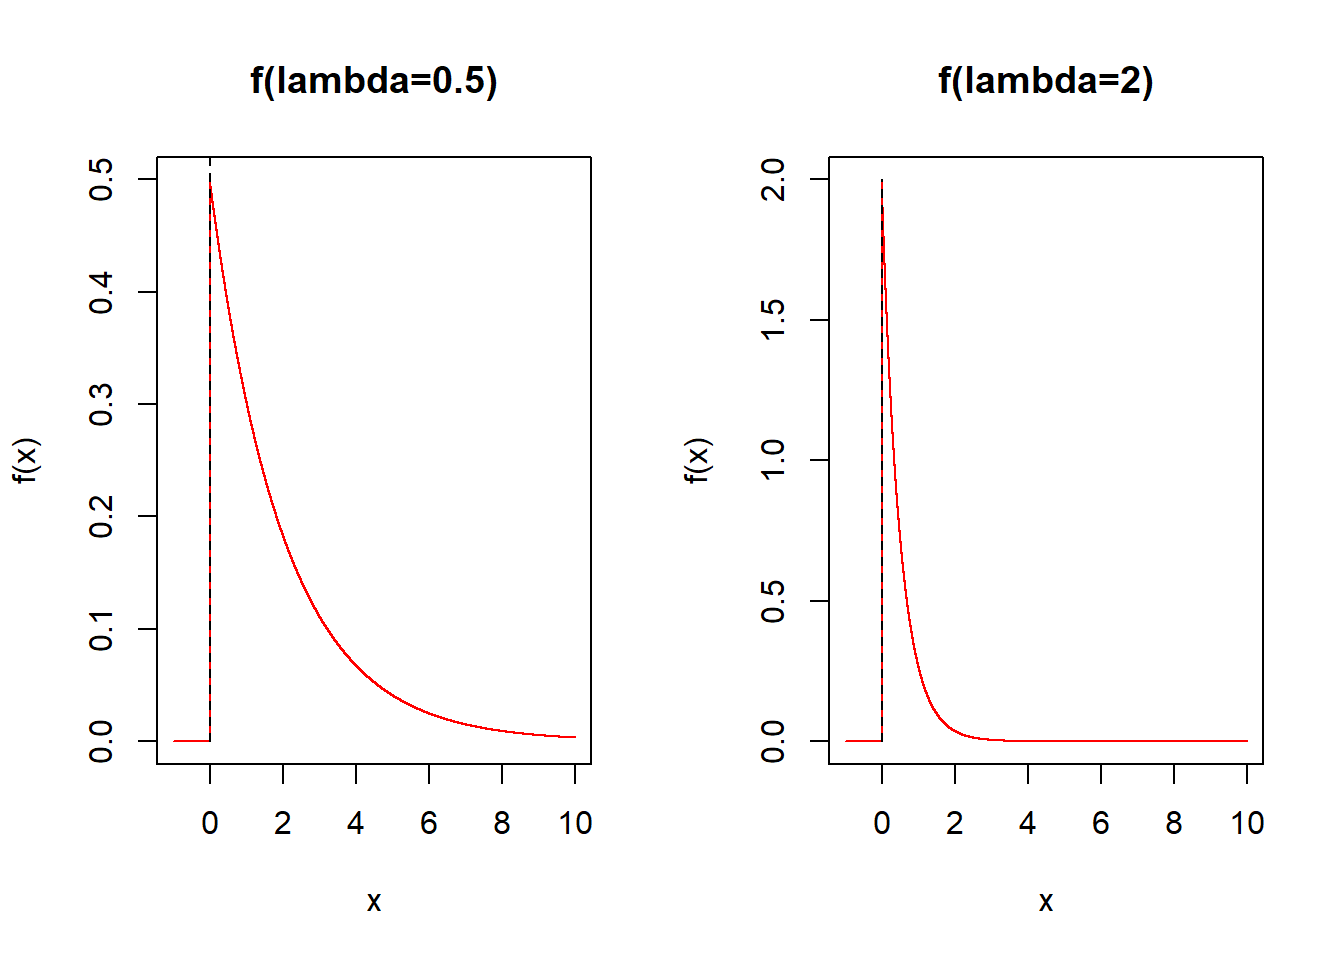
\includegraphics{_main_files/figure-latex/unnamed-chunk-62-1.pdf}

\begin{center}\rule{0.5\linewidth}{0.5pt}\end{center}

\begin{center}\rule{0.5\linewidth}{0.5pt}\end{center}

\hypertarget{distribuciuxf3n-exponencial}{%
\section{Distribución exponencial}\label{distribuciuxf3n-exponencial}}

En un proceso de Poisson: ¿Cuál es la probabilidad de observar una distancia \textbf{menor} que \(a\) hasta el primer event?

Recuerde que esta probabilidad \(F(a)=P(X \leq a)\) es la densidad de probabilidad

\[F(a)=\lambda\int_\infty^a e^{-x\lambda}dx=1-e^{-a\lambda}\]

\begin{itemize}
\tightlist
\item
  ¿Cuál es la probabilidad de observar una distancia \textbf{mayor} que \(a\) hasta el primer evento?
\end{itemize}

\[P(X > a)=1- P(X \leq a)= 1- F(a) = e^{-a\lambda}\]

\begin{center}\rule{0.5\linewidth}{0.5pt}\end{center}

\begin{center}\rule{0.5\linewidth}{0.5pt}\end{center}

\hypertarget{distribuciuxf3n-exponencial-1}{%
\section{Distribución exponencial}\label{distribuciuxf3n-exponencial-1}}

Con la función de densidad exponencial:

\[f(x)=\lambda e^{-\lambda x}\]

Podemos responder preguntas como:

\begin{itemize}
\tightlist
\item
  ¿Cuál es la probabilidad de que tengamos que esperar un bus por más de \(1\) hora cuando en promedio hay dos buses por hora?
\end{itemize}

\[P(X > 1)=1-P(X \le 1) = 1-F(1,\lambda=2)=0.1353\]

en R 1-pexp(1,2)

\begin{itemize}
\tightlist
\item
  ¿Cuál es la probabilidad de tener que esperar menos de \(2\) segundos para detectar una partícula cuando la tasa de desintegración radiactiva es de \(2\) partículas cada segundo? \(F(2,\lambda=2)\)
\end{itemize}

\[P(X\le 2)=F(2,\lambda=2)=0.981\]

en R pexp(2,2)

\begin{center}\rule{0.5\linewidth}{0.5pt}\end{center}

\begin{center}\rule{0.5\linewidth}{0.5pt}\end{center}

\hypertarget{distribuciuxf3n-exponencial-2}{%
\section{Distribución exponencial}\label{distribuciuxf3n-exponencial-2}}

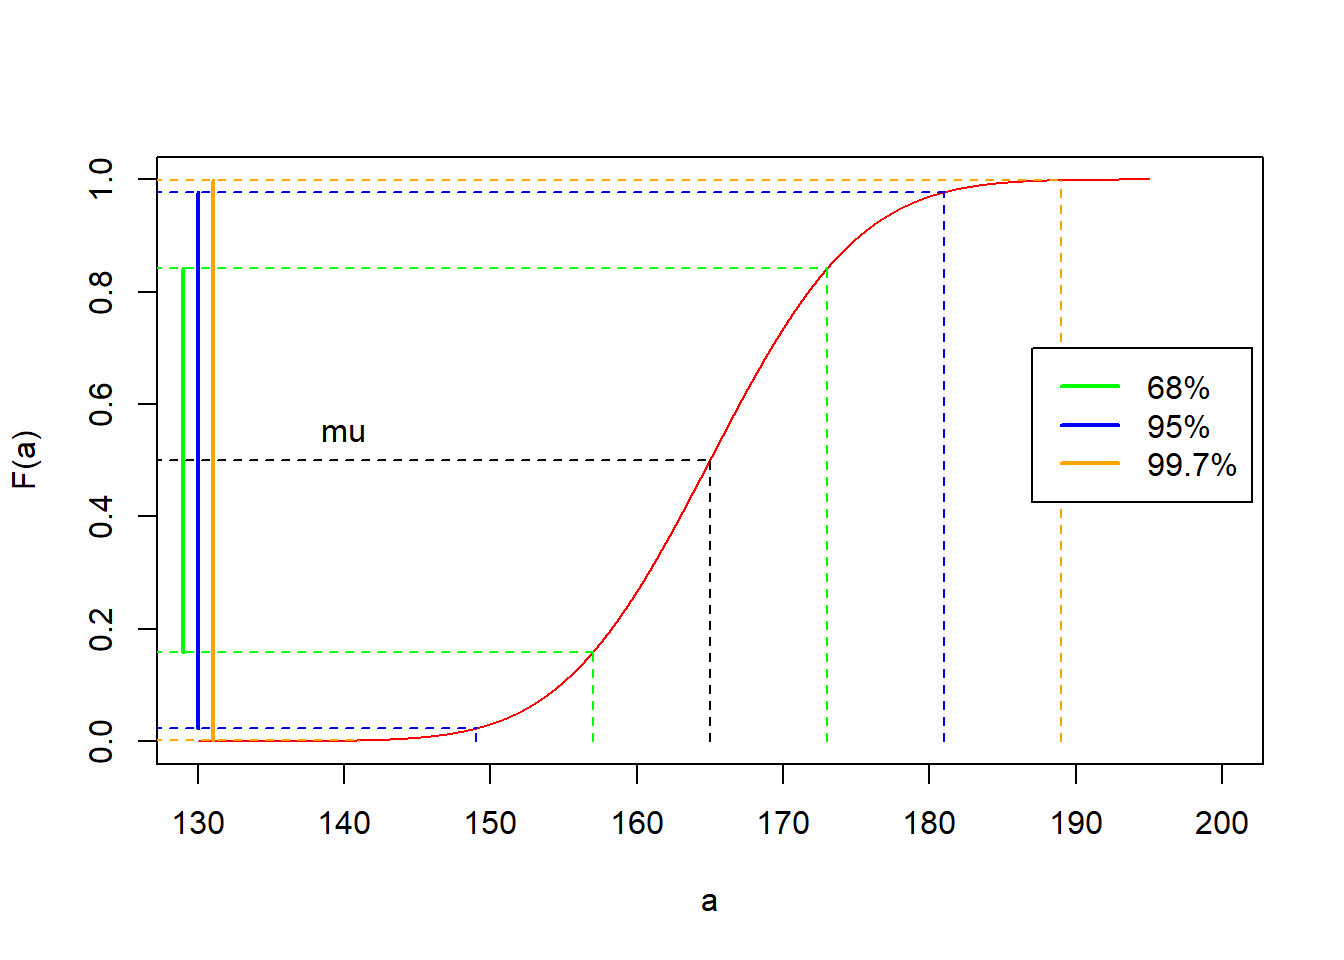
\includegraphics{_main_files/figure-latex/unnamed-chunk-63-1.pdf}

La mediana \(x_m\) es tal que \(F(x_m)=0.5\). Eso es \(x_m=\frac{\log(2)}{\lambda}\)

\hypertarget{distribuciuxf3n-normal}{%
\chapter{Distribución normal}\label{distribuciuxf3n-normal}}

\hypertarget{objetivo-8}{%
\section{Objetivo}\label{objetivo-8}}

Modelo de probabilidad para valiables continuas:

\begin{itemize}
\tightlist
\item
  Distribución normal
\end{itemize}

\begin{center}\rule{0.5\linewidth}{0.5pt}\end{center}

\begin{center}\rule{0.5\linewidth}{0.5pt}\end{center}

\hypertarget{modelo-de-probabilidad-para-valiables-continuas}{%
\section{Modelo de probabilidad para valiables continuas}\label{modelo-de-probabilidad-para-valiables-continuas}}

Modelo de probabilidad para valiables continuas son funciones de densidad de probabilidad \(f(x)\) de variables aleatorias continuas que \textbf{creemos} describen experimentos aleatorios reales.

Definición:

Positiva:

\begin{itemize}
\tightlist
\item
  \(f(x) \geq 0\)
\end{itemize}

\emph{Permite calcular probabilidades usando el área bajo la curva:}

\begin{itemize}
\tightlist
\item
  \(P(a\leq X \leq b)=\int_{a}^{b} f(x) dx\)
\end{itemize}

La probabilidad de algún valor es \(1\):

\begin{itemize}
\tightlist
\item
  \(\int_{-\infty}^{\infty} f(x) dx = 1\)
\end{itemize}

\begin{center}\rule{0.5\linewidth}{0.5pt}\end{center}

\begin{center}\rule{0.5\linewidth}{0.5pt}\end{center}

\hypertarget{densidad-normal}{%
\section{Densidad normal}\label{densidad-normal}}

En 1801 Gauss analizó la órbita de Ceres (gran asteroide entre Marte y Júpiter).

\begin{itemize}
\tightlist
\item
  La gente sospechaba que era un nuevo planeta.
\item
  Las medidas tenían errores.
\item
  Le interesaba saber cómo se distribuían las observaciones para poder encontrar la órbita más probable.
\item
  Quería predecir hacia dónde deberían apuntar los astrónomos sus telescopios para encontrarlo unos meses después de que hubiera pasado por detrás del Sol.
\end{itemize}

\begin{center}\rule{0.5\linewidth}{0.5pt}\end{center}

\begin{center}\rule{0.5\linewidth}{0.5pt}\end{center}

\hypertarget{densidad-normal-1}{%
\section{Densidad normal}\label{densidad-normal-1}}

Errores debidos a la medición.

\begin{center}\rule{0.5\linewidth}{0.5pt}\end{center}

\begin{center}\rule{0.5\linewidth}{0.5pt}\end{center}

\hypertarget{densidad-normal-2}{%
\section{Densidad normal}\label{densidad-normal-2}}

Él asumió que

\begin{itemize}
\tightlist
\item
  los errores pequeños eran más probables que los errores grandes
\item
  el error a una distancia \(-\epsilon\) o \(\epsilon\) de la medida más probable era igualmente probable
\item
  la altitud más \textbf{probable} de Ceres en un momento dado en el cielo era el \textbf{promedio} de varias mediciones de altitud en esa latitud.
\end{itemize}

\begin{center}\rule{0.5\linewidth}{0.5pt}\end{center}

\begin{center}\rule{0.5\linewidth}{0.5pt}\end{center}

\hypertarget{densidad-normal-3}{%
\section{Densidad normal}\label{densidad-normal-3}}

Eso fue suficiente para mostrar que las desviaciones aleatorias \(y\) \textbf{de la órbita} distribuidas como

\[f(y)=\frac{h}{\sqrt{\pi}}e^{-h^2y^2}\]

*La evolución de la distribución Normal, Saul Stahl, Revista de Matemáticas, 2006.

\begin{center}\rule{0.5\linewidth}{0.5pt}\end{center}

\begin{center}\rule{0.5\linewidth}{0.5pt}\end{center}

\hypertarget{densidad-normal-4}{%
\section{Densidad normal}\label{densidad-normal-4}}

Escribamos la distribución de errores

\[f(y)=\frac{h}{\sqrt{\pi}}e^{-h^2y^2}\]

para los errores de medidas desde el horizonte \(X\) entonces \(y=x-x_0\)

\[f(x)=\frac{h}{\sqrt{\pi}}e^{-h^2(x-x_0)^2}\]

\begin{itemize}
\tightlist
\item
  La \textbf{media} de esta densidad de probabilidad es:
\end{itemize}

\(E(X)=\mu=x_0\), que representa la \textbf{verdadera} posición de Ceres desde el horizonte (propiedad del sistema físico).

\begin{itemize}
\tightlist
\item
  La \textbf{varianza} es:
\end{itemize}

\(V(X)=\sigma^2=\frac{1}{2h^2}\), que representa la dispersión del error en las observaciones (propiedad del sistema de medida).

\begin{center}\rule{0.5\linewidth}{0.5pt}\end{center}

\begin{center}\rule{0.5\linewidth}{0.5pt}\end{center}

\hypertarget{definiciuxf3n}{%
\section{Definición}\label{definiciuxf3n}}

Una variable aleatoria \(X\) definida en los números reales tiene una densidad \textbf{Normal} si toma la forma

\[f(x; \mu, \sigma^2)=\frac{1}{\sqrt{2\pi}\sigma}e^{-\frac{(x-\mu)^2}{2\sigma^2}}, x \in  {\Bbb R}\]

con media y varianza:

\begin{itemize}
\tightlist
\item
  \(E(X) = \mu\)
\item
  \(V (X) = \sigma^2\)
\end{itemize}

\(\mu\) y \(\sigma\) son los \textbf{dos parámetros} que describen completamente la función de densidad normal y su \textbf{interpretación} depende del experimento aleatorio.

Cuando \(X\) sigue una densidad Normal, es decir, se distribuye normalmente, escribimos

\[X\rightarrow N(\mu,\sigma^2)\]

\begin{center}\rule{0.5\linewidth}{0.5pt}\end{center}

\begin{center}\rule{0.5\linewidth}{0.5pt}\end{center}

\hypertarget{densidad-de-probabilidad-normal-gaussiana}{%
\section{Densidad de probabilidad normal (gaussiana)}\label{densidad-de-probabilidad-normal-gaussiana}}

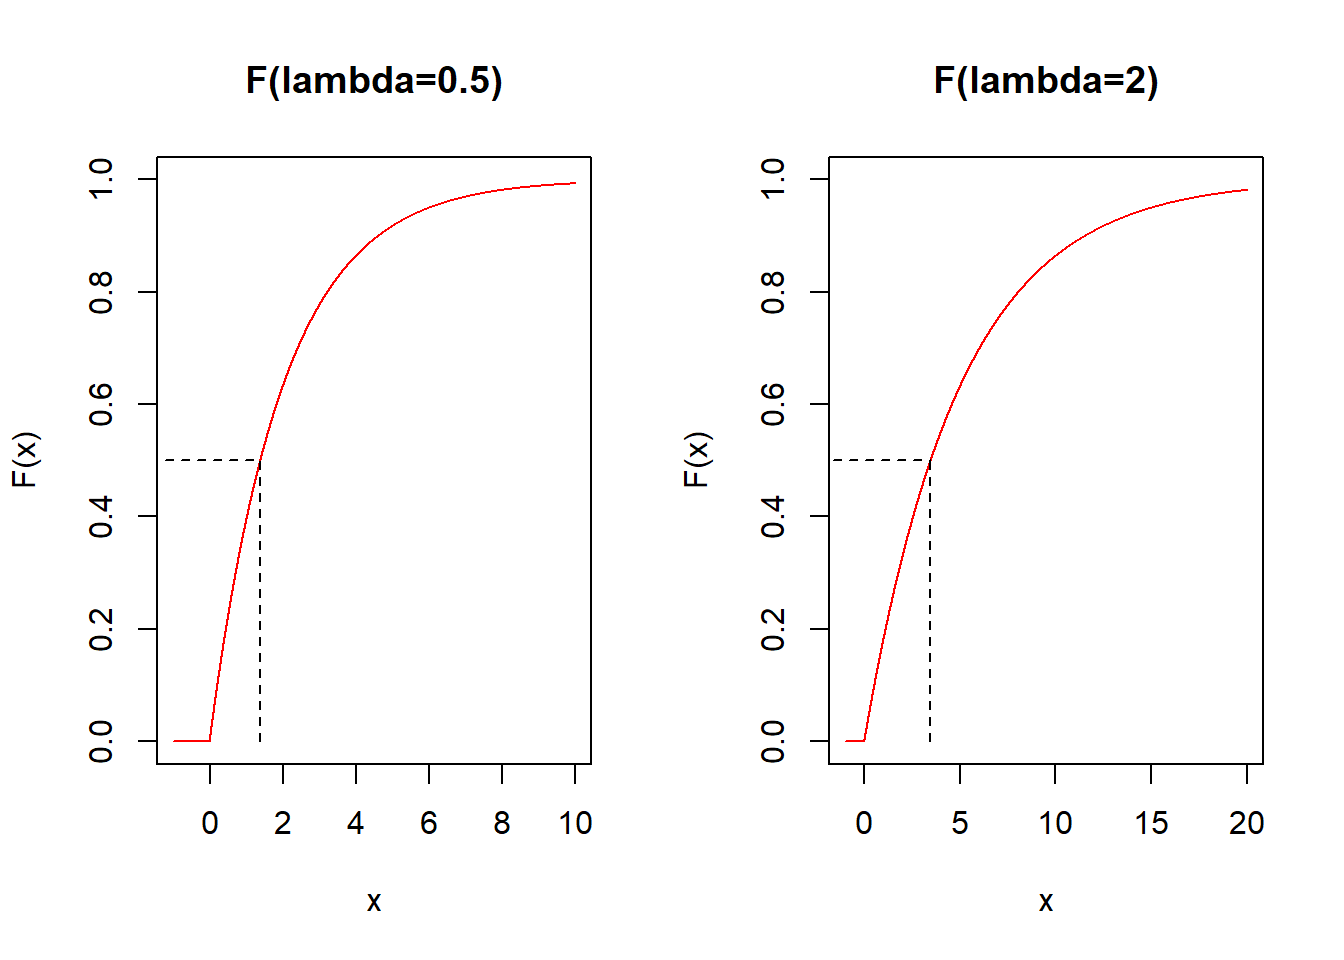
\includegraphics{_main_files/figure-latex/unnamed-chunk-64-1.pdf}

\begin{center}\rule{0.5\linewidth}{0.5pt}\end{center}

\begin{center}\rule{0.5\linewidth}{0.5pt}\end{center}

\hypertarget{distribuciuxf3n-normal-1}{%
\section{Distribución normal}\label{distribuciuxf3n-normal-1}}

La distribución de probabilidad de la densidad Normal:

\[F_{normal}(a)=P(Z \leq a)\]

es la función de \textbf{error} definida por el área bajo la curva de \(-\infty\) a \(a\)

\[F_{normal}(a)=\int_{-\infty}^{a}\frac{1}{\sqrt{2\pi}\sigma}e^{-\frac{(x-\mu) ^2}{2\sigma^2}} dx\]
La función se encuentra en la mayoría de los programas informáticos.

\begin{center}\rule{0.5\linewidth}{0.5pt}\end{center}

\begin{center}\rule{0.5\linewidth}{0.5pt}\end{center}

\hypertarget{distribuciuxf3n-normal-2}{%
\section{Distribución normal}\label{distribuciuxf3n-normal-2}}

Cuando \[X \rightarrow N(\mu, \sigma^2)\]

Podemos hacer preguntas como:

\begin{itemize}
\tightlist
\item
  ¿Cuál es la probabilidad de que una mujer en la población mida como máximo \(150 cm\) de altura si las mujeres tienen una altura media de \(165 cm\) con una desviación estándar de \(8 cm\)?
\end{itemize}

\(P(X\le 150)=F(150, \mu=165, \sigma=8)=0.03039636\)

in R pnorm(150, 165, 8)
- ¿Cuál es la probabilidad de que la altura de una mujer en la población esté entre \(165cm\) y \(170cm\)?

\(P(165 \le X \le 170)=F(170, \mu=165, \sigma=8)-F(165, \mu=165, \sigma=8)=0.2340145\)

in R pnorm(170, 165, 8)-pnorm(165, 165, 8)

\begin{center}\rule{0.5\linewidth}{0.5pt}\end{center}

\begin{center}\rule{0.5\linewidth}{0.5pt}\end{center}

\hypertarget{distribuciuxf3n-normal-3}{%
\section{Distribución normal}\label{distribuciuxf3n-normal-3}}

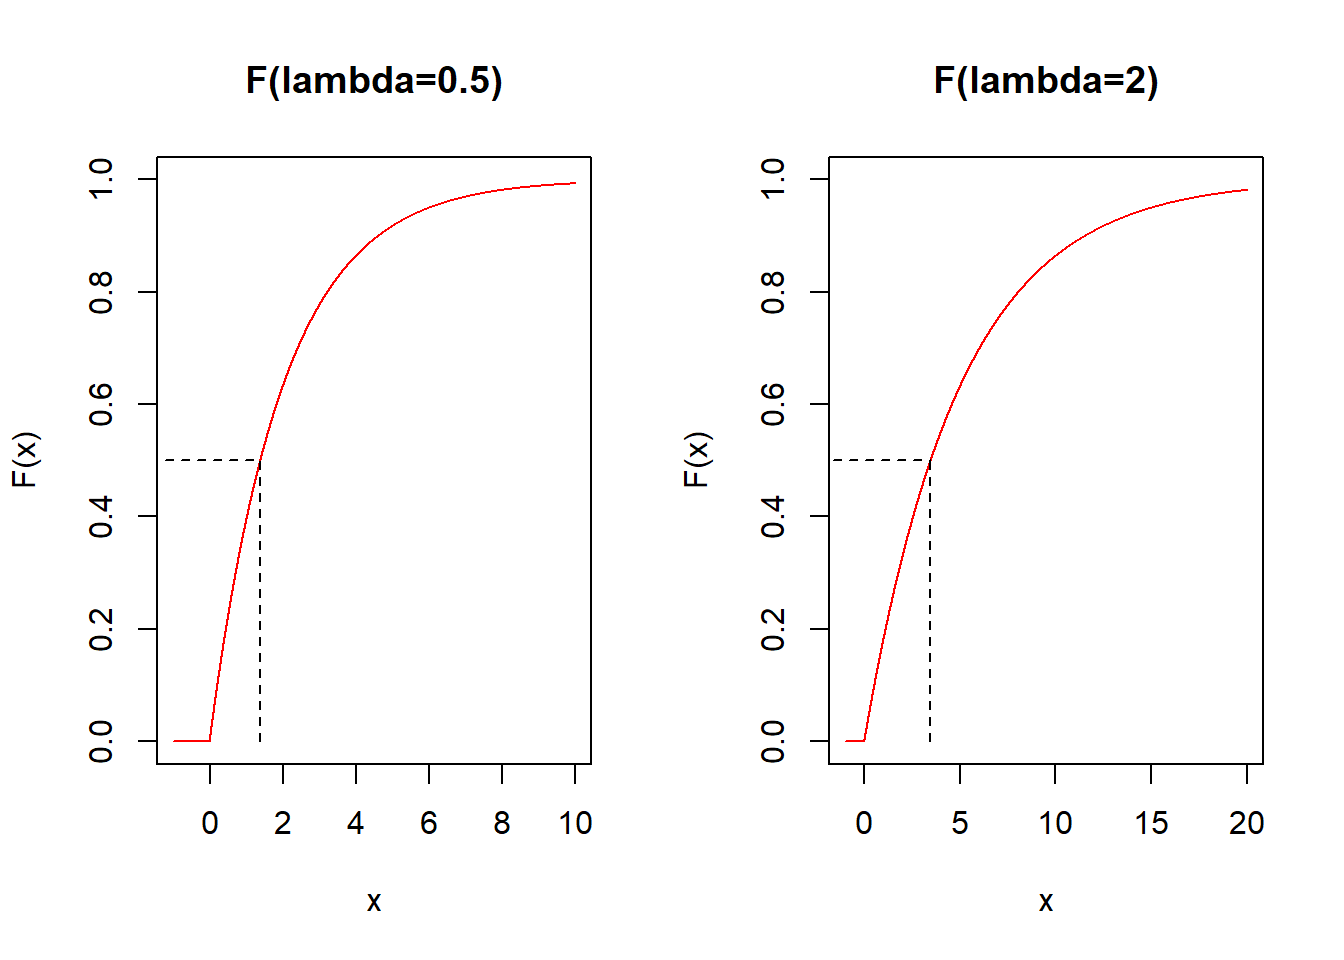
\includegraphics{_main_files/figure-latex/unnamed-chunk-65-1.pdf}

\begin{center}\rule{0.5\linewidth}{0.5pt}\end{center}

\begin{center}\rule{0.5\linewidth}{0.5pt}\end{center}

\hypertarget{distribuciuxf3n-normal-4}{%
\section{Distribución normal}\label{distribuciuxf3n-normal-4}}

\begin{itemize}
\tightlist
\item
  la media \(\mu\) es también la mediana ya que divide las medidas en dos
\item
  Los valores de \(x\) que caen más allá de 2\(\sigma\) se consideran \textbf{raros} \(5\%\)
\item
  Los valores de \(x\) que caen más allá de 3\(\sigma\) se consideran \textbf{extremadamente raros} \(0.2\%\)
\end{itemize}

\begin{center}\rule{0.5\linewidth}{0.5pt}\end{center}

\begin{center}\rule{0.5\linewidth}{0.5pt}\end{center}

\hypertarget{distribuciuxf3n-normal-5}{%
\section{Distribución normal}\label{distribuciuxf3n-normal-5}}

Podemos definir los límites de \textbf{observaciones comunes} para la distribución de la altura de las mujeres en la población.

\begin{itemize}
\tightlist
\item
  \(P(165-8 \leq X \leq 165+8)=P(157 \leq X \leq 173)=0.68\)
\item
  \(P(165-2 \times 8 \leq X \leq 165+2\times 8)=P(149 \leq X \leq 181)=0.95\)
\item
  \(P(165-3 \times 8 \leq X \leq 165+3\times 8)=P(141 \leq X \leq 189)=0.997\)
\end{itemize}

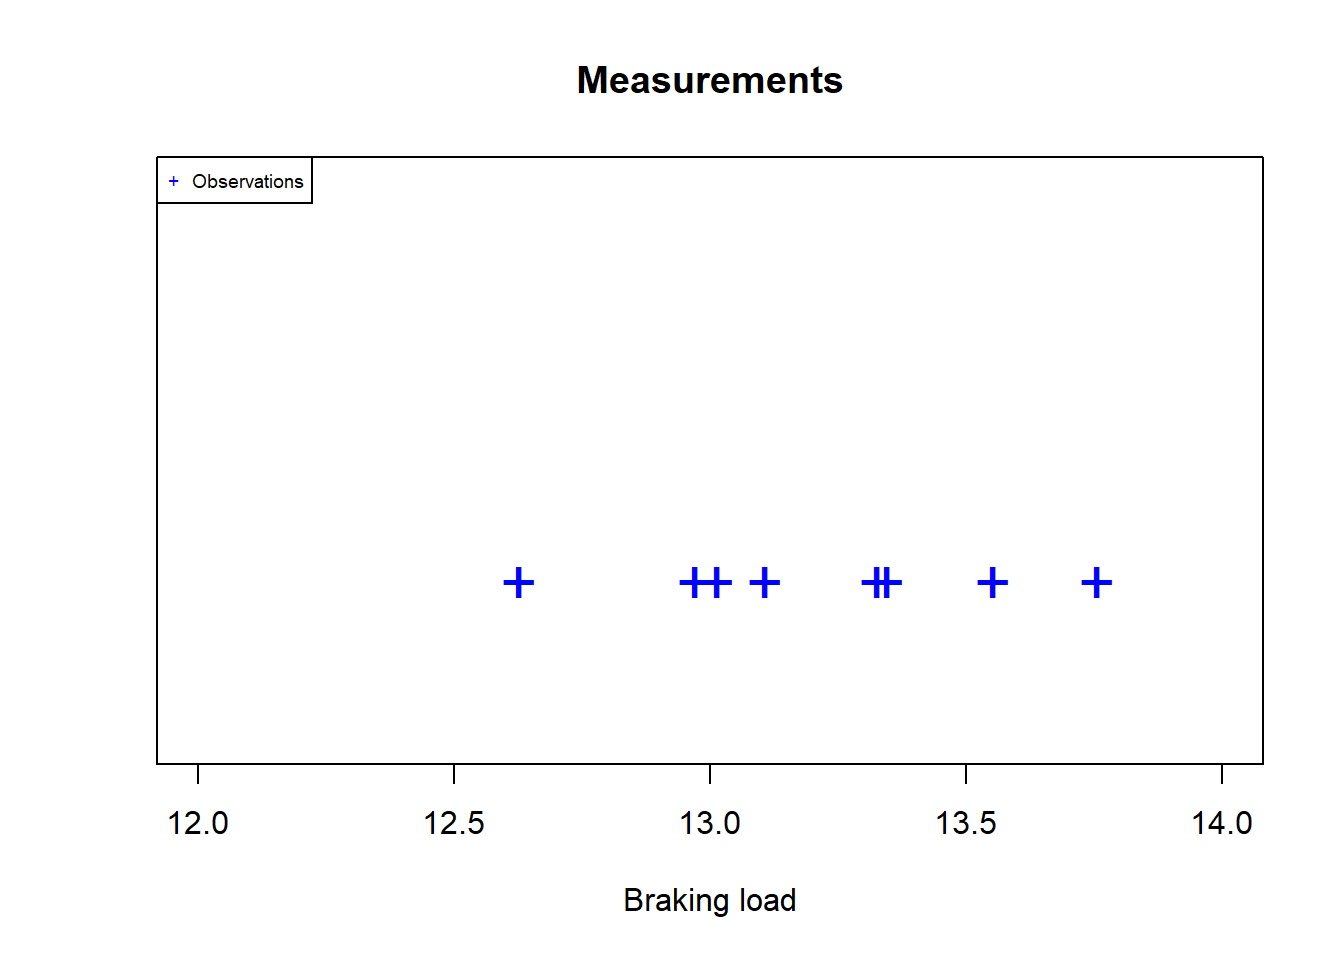
\includegraphics{_main_files/figure-latex/unnamed-chunk-66-1.pdf}

\begin{center}\rule{0.5\linewidth}{0.5pt}\end{center}

\begin{center}\rule{0.5\linewidth}{0.5pt}\end{center}

\hypertarget{densidad-normal-estuxe1ndar}{%
\section{Densidad normal estándar}\label{densidad-normal-estuxe1ndar}}

Cambiemos las variables a una \textbf{variable estandarizada}

\[Z=\frac{X-\mu}{\sigma}\]

en la densidad

\[f(x; \mu, \sigma^2)=\frac{1}{\sqrt{2\pi}\sigma}e^{-\frac{(x-\mu)^2}{2\sigma^2}}, x \in {\Bbb R}\]

reemplazando \(x=\sigma z+\mu\) y \(dx=\sigma dz\) en la expresión de probabilidad que tenemos

\(P(x\leq X \leq x +dx)=P(z\leq Z \leq z +dz)\)
\[=\frac{1}{\sqrt{2\pi}\sigma}e^{-\frac{(x-\mu)^2}{2\sigma^2}}dx\] \[=\frac{1}{ \sqrt{2\pi}}e^{-\frac{z^2}{2}} dz\]

obtenemos la forma \textbf{estandarizada} de la densidad normal.

\begin{center}\rule{0.5\linewidth}{0.5pt}\end{center}

\begin{center}\rule{0.5\linewidth}{0.5pt}\end{center}

\hypertarget{densidad-normal-estuxe1ndar-1}{%
\section{Densidad normal estándar}\label{densidad-normal-estuxe1ndar-1}}

\textbf{Definición}

Una variable aleatoria \(Z\) definida en los números reales tiene una densidad \textbf{estándar} si toma la forma

\[f(z)=\frac{1}{\sqrt{2\pi}}e^{-\frac{z^2}{2}} dz,z \in {\Bbb R}\]

con media y varianza

\begin{itemize}
\item
  \(E(X) = 0\)
\item
  \(V (X) =1\).
\end{itemize}

\begin{center}\rule{0.5\linewidth}{0.5pt}\end{center}

\begin{center}\rule{0.5\linewidth}{0.5pt}\end{center}

\hypertarget{densidad-normal-estuxe1ndar-2}{%
\section{Densidad normal estándar}\label{densidad-normal-estuxe1ndar-2}}

La densidad estándar:

\[f(z)=\frac{1}{\sqrt{2\pi}}e^{-\frac{z^2}{2}} dz,z \in {\Bbb R}\]

\begin{itemize}
\item
  es la densidad normal \(N(\mu=0,\sigma^2=1)\)
\item
  cualquier variable distribuida normalmente \(X\) puede transformarse en una variable \(Z\)
\end{itemize}

\[Z=\frac{x-\mu}{\sigma}\]

que sigue una distribución estándar:

\[Z \rightarrow N(0,1)\]

\begin{center}\rule{0.5\linewidth}{0.5pt}\end{center}

\begin{center}\rule{0.5\linewidth}{0.5pt}\end{center}

\hypertarget{distribuciuxf3n-normal-6}{%
\section{Distribución normal}\label{distribuciuxf3n-normal-6}}

Todas las densidades normales se pueden obtener a partir de la densidad estándar con los valores de \(\mu\) y \(\sigma\)

\begin{center}\rule{0.5\linewidth}{0.5pt}\end{center}

\begin{center}\rule{0.5\linewidth}{0.5pt}\end{center}

\hypertarget{distribuciuxf3n-estuxe1ndar}{%
\section{Distribución estándar}\label{distribuciuxf3n-estuxe1ndar}}

La distribución de probabilidad de la densidad estándar:

\[\phi(a)=F_{estándar}(a)=P(Z \leq a)\]

es la función \textbf{error} definida por

\[\phi(a)=\int_{-\infty}^{a} \frac{1}{\sqrt{2\pi}}e^{-\frac{z^2}{2}} dz\]

You can find it in most computer programs

\begin{center}\rule{0.5\linewidth}{0.5pt}\end{center}

\begin{center}\rule{0.5\linewidth}{0.5pt}\end{center}

\hypertarget{standard-normal-density}{%
\section{Standard normal density}\label{standard-normal-density}}

\begin{center}\rule{0.5\linewidth}{0.5pt}\end{center}

\begin{center}\rule{0.5\linewidth}{0.5pt}\end{center}

\hypertarget{densidad-normal-estuxe1ndar-3}{%
\section{Densidad normal estándar}\label{densidad-normal-estuxe1ndar-3}}

Definimos los límites de las \textbf{observaciones más comunes} para la variable estándar

\begin{itemize}
\tightlist
\item
  \(P(-0.67 \leq X \leq 0.67)=0.50\)
\item
  \(P(-1.96 \leq X \leq 1.96)=0.95\)
\item
  \(P(-2.58 \leq X \leq 2.58)=0.99\)
\end{itemize}

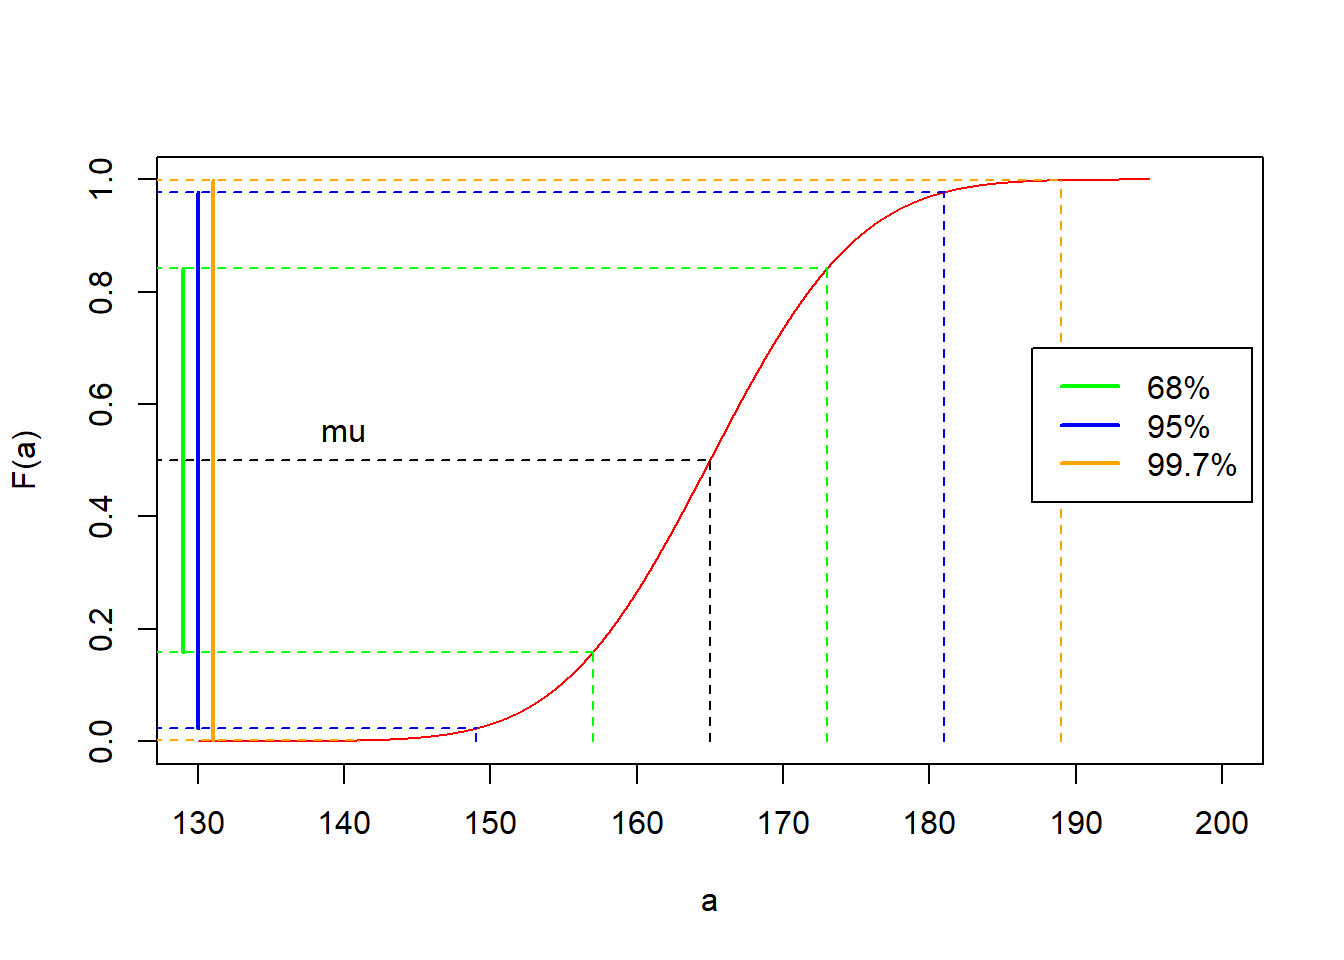
\includegraphics{_main_files/figure-latex/unnamed-chunk-67-1.pdf}

\begin{center}\rule{0.5\linewidth}{0.5pt}\end{center}

\begin{center}\rule{0.5\linewidth}{0.5pt}\end{center}

\hypertarget{distribuciones-normal-y-estuxe1ndar}{%
\section{Distribuciones normal y estándar}\label{distribuciones-normal-y-estuxe1ndar}}

Para cualquier variable normalmente distribuida \(X\), tal que

\[X\rightarrow N(\mu, \sigma^2)\]

su distribución \(F(a)=P(X \leq a)\) se puede calcular a partir de

\[F(a)= \phi \big(\frac{a-\mu}{\sigma}\big)\]

\begin{center}\rule{0.5\linewidth}{0.5pt}\end{center}

\begin{center}\rule{0.5\linewidth}{0.5pt}\end{center}

\hypertarget{distribuciuxf3n-normal-7}{%
\section{Distribución normal}\label{distribuciuxf3n-normal-7}}

Para calcular \(P(a\leq X \leq b)\), usamos la propiedad de las distribuciones de probabilidad

\[F(b)-F(a)=P(X\leq b)-P(X\leq a)\]

estandaricemos

\(=P(\frac{X-\mu}{\sigma}\leq \frac{a-\mu}{\sigma})-P(\frac{X-\mu}{\sigma}\leq \frac{b-\mu}{\sigma})\)

\(=P(Z \leq \frac{b-\mu}{\sigma})-P(Z \leq \frac{a-\mu}{\sigma}\big)\)

\(=\phi \big(\frac{b-\mu}{\sigma}\big)-\phi \big(\frac{a-\mu}{\sigma}\big)\)

Entonces

\[F(b)-F(a)=\phi \big(\frac{b-\mu}{\sigma}\big)-\phi \big(\frac{a-\mu}{\sigma}\big)\]
Las probabilidades de \textbf{cualquier variable normal} se pueden obtener de la \textbf{distribución estándar}, después de la estandarización (restar la media y dividir por la desviación estándar).

\begin{center}\rule{0.5\linewidth}{0.5pt}\end{center}

\begin{center}\rule{0.5\linewidth}{0.5pt}\end{center}

\hypertarget{resumen-de-modelos-de-probabilidad}{%
\section{Resumen de modelos de probabilidad}\label{resumen-de-modelos-de-probabilidad}}

\begin{longtable}[]{@{}
  >{\centering\arraybackslash}p{(\columnwidth - 10\tabcolsep) * \real{0.17}}
  >{\centering\arraybackslash}p{(\columnwidth - 10\tabcolsep) * \real{0.19}}
  >{\centering\arraybackslash}p{(\columnwidth - 10\tabcolsep) * \real{0.19}}
  >{\centering\arraybackslash}p{(\columnwidth - 10\tabcolsep) * \real{0.17}}
  >{\centering\arraybackslash}p{(\columnwidth - 10\tabcolsep) * \real{0.14}}
  >{\centering\arraybackslash}p{(\columnwidth - 10\tabcolsep) * \real{0.14}}@{}}
\toprule
\begin{minipage}[b]{\linewidth}\centering
Modelo
\end{minipage} & \begin{minipage}[b]{\linewidth}\centering
X
\end{minipage} & \begin{minipage}[b]{\linewidth}\centering
rango de x
\end{minipage} & \begin{minipage}[b]{\linewidth}\centering
f(x)
\end{minipage} & \begin{minipage}[b]{\linewidth}\centering
E(X)
\end{minipage} & \begin{minipage}[b]{\linewidth}\centering
V(X)
\end{minipage} \\
\midrule
\endhead
Uniforme & número entero o real & \([a,b]\) & \(\frac{1}{n}\) & \(\frac{b+a}{2}\) & \(\frac{(b-a+1)^2-1}{12}\) \\
Bernoulli & evento A & 0,1 & \((1-p)^{1-x}p^x\) & \(p\) & \(p(1-p)\) \\
binomial & \# de eventos A en \(n\) repeticiones de ensayos de Bernoulli & 0,1,\ldots{} & \(\binom n x (1-p)^{n-x}p^x\) & \(np\) & \(np(1-p)\) \\
Binomial negativo para eventos & \# de eventos B en repeticiones de Bernoulli antes de \(r\) As & 0,1,.. & \(\binom {x+r-1} x (1-p)^xp^r\) & \(\frac{r(1-p)}{p}\) & \(\frac{r(1-p)}{p^2}\) \\
Hipergeométrico & \# eventos A en una muestra \(n\) de la población \(N\) con \(K\) As & \(\max(0, n+K-N)\), \ldots{} \(\min(K, n)\) & \(\frac{1}{\binom N n}\binom K x \binom {N-K} {n-x}\) & \(n*\frac{N}{K}\) & \(n \frac{N}{K} (1-\frac{N}{K})\frac{N-n}{N-1}\) \\
Poisson & \# de eventos A en un intervalo & 0,1, .. & \(\frac{e^{-\lambda}\lambda^x}{x!}\) & \(\lambda\) & \(\lambda\) \\
Exponencial & Intervalo entre dos eventos A & \([0,\infty)\) & \(\lambda e^{-\lambda x}\) & \(\frac{1}{\lambda}\) & \(\frac{1}{\lambda^2}\) \\
Normal & medida con errores simétricos cuyo valor más probable es la media & \((-\infty, \infty)\) & \(\frac{1}{\sqrt{2\pi}\sigma}e^{-\frac{(x-\mu)^2}{2\sigma^2 }}\) & \(\mu\) & \(\sigma^2\) \\
\bottomrule
\end{longtable}

\begin{center}\rule{0.5\linewidth}{0.5pt}\end{center}

\begin{center}\rule{0.5\linewidth}{0.5pt}\end{center}

\hypertarget{funciones-r-para-modelos-de-probabilidad}{%
\section{Funciones R para modelos de probabilidad}\label{funciones-r-para-modelos-de-probabilidad}}

\begin{longtable}[]{@{}lc@{}}
\toprule
Modelo & R \\
\midrule
\endhead
Uniforme (continuo) & dunif(x, a, b) \\
binomial & dbimon(x,n,p) \\
Binomial negativo para eventos & dnbinom(x,r,p) \\
Hipergeométrico & dhyper(x, K, N-K, n) \\
Poisson & dpois(x, lambda) \\
Exponencial & dexp(x, lambda) \\
Normal & dnomr(x, mu, sigma) \\
\bottomrule
\end{longtable}

\hypertarget{distribuciones-de-muestreo}{%
\chapter{Distribuciones de muestreo}\label{distribuciones-de-muestreo}}

\hypertarget{objetivo-9}{%
\section{Objetivo}\label{objetivo-9}}

Distribuciones para

\begin{itemize}
\tightlist
\item
  Media (promedio) muestral
\item
  suma muestral
\item
  Varianza muestral
\end{itemize}

\begin{center}\rule{0.5\linewidth}{0.5pt}\end{center}

\begin{center}\rule{0.5\linewidth}{0.5pt}\end{center}

\hypertarget{distribuciuxf3n-normal-8}{%
\section{Distribución normal}\label{distribuciuxf3n-normal-8}}

Cuando tenemos una variable aleatoria normal

\[X \rightarrow N(x; \mu, \sigma^2)\]

¿Cómo estimamos \(\mu\) y \(\sigma^2\)?

\begin{itemize}
\item
  necesitamos tomar una \textbf{muestra aleatoria}
\item
  necesitamos \textbf{estimar} cada parámetro
\end{itemize}

\begin{center}\rule{0.5\linewidth}{0.5pt}\end{center}

\begin{center}\rule{0.5\linewidth}{0.5pt}\end{center}

\hypertarget{ejemplo-cuando-no-conocemos-los-parametros}{%
\section{Ejemplo: Cuando no conocemos los parametros}\label{ejemplo-cuando-no-conocemos-los-parametros}}

Imaginemos que un cliente que nos pide a nuestra empresa metalúrgica que le vendamos \(8\) cables que pueden cargar hasta \(96\) Toneladas; eso es \(12\) Toneladas cada uno.

\begin{itemize}
\tightlist
\item
  Tenemos en \textbf{stock} un conjunto de cables que podrían hacer el trabajo.
\end{itemize}

¿Podemos utilizar los cables en stock o necesitaríamos producir unos nuevos?

\begin{center}\rule{0.5\linewidth}{0.5pt}\end{center}

\begin{center}\rule{0.5\linewidth}{0.5pt}\end{center}

\hypertarget{ejemplo-12}{%
\section{Ejemplo}\label{ejemplo-12}}

Tomamos una muestra de \(8\) experimentos aleatorios, cada uno de los cuales consiste en cargar un cable hasta que se rompa y anotamos la carga de rotura.

Estos son los resultados: La observación de una \textbf{muestra} de tamaño \(8\)

\begin{verbatim}
## [1] 13.34642 13.32620 13.01459 13.10811 12.96999 13.55309 13.75557 12.62747
\end{verbatim}

\begin{itemize}
\item
  Ninguno se rompió a \(12\) Toneladas.
\item
  Hubo uno que se rompió a \(12.62747\) Toneladas.
\end{itemize}

¿Nos arriesgamos y vendemos una muestra aleatoria \(8\) cables de nuestro inventario?

\begin{center}\rule{0.5\linewidth}{0.5pt}\end{center}

\begin{center}\rule{0.5\linewidth}{0.5pt}\end{center}

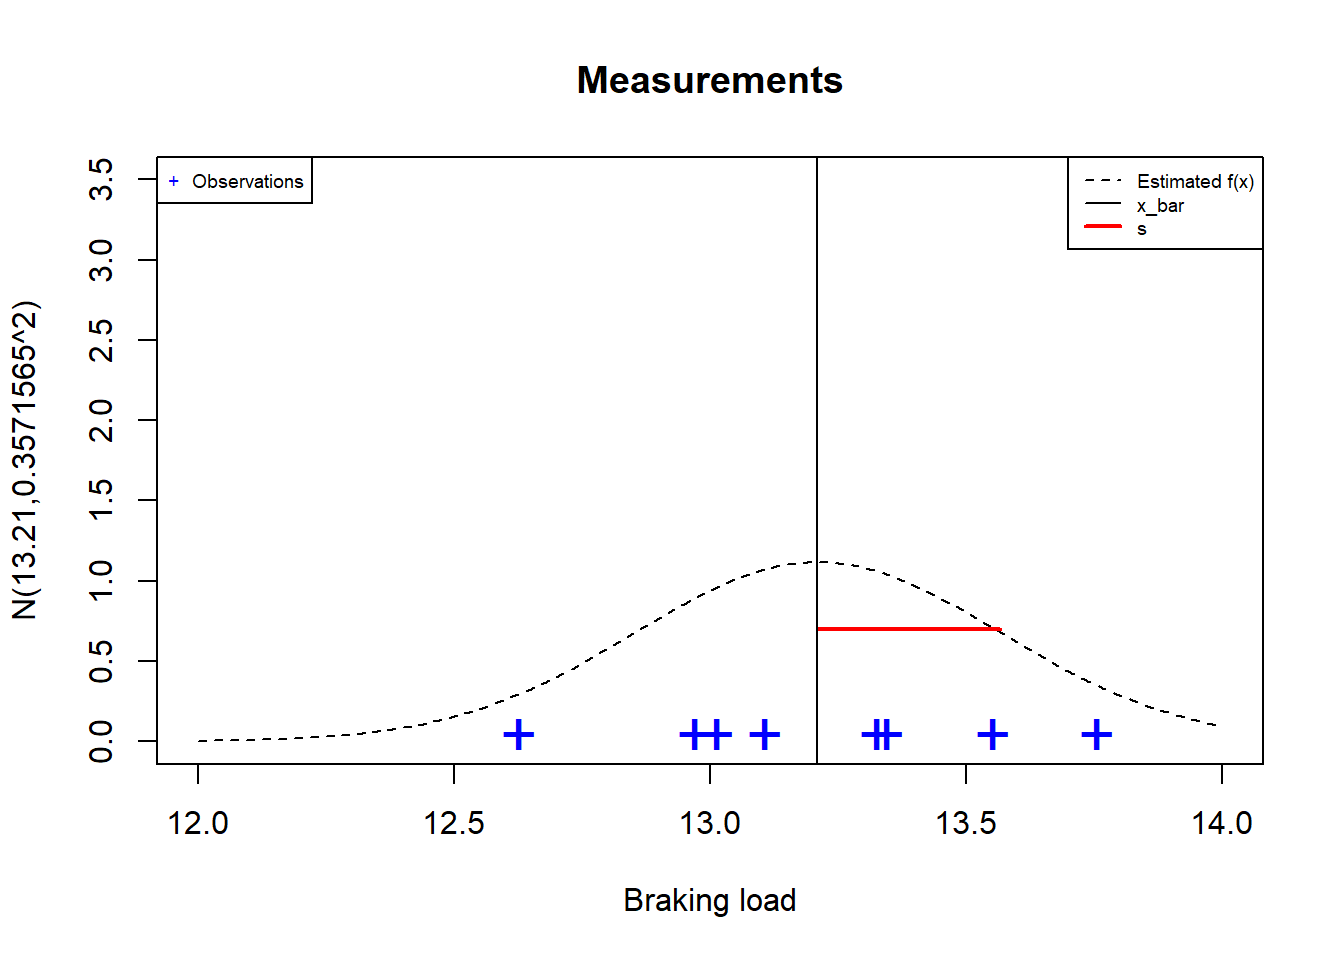
\includegraphics{_main_files/figure-latex/unnamed-chunk-69-1.pdf}

\begin{center}\rule{0.5\linewidth}{0.5pt}\end{center}

\begin{center}\rule{0.5\linewidth}{0.5pt}\end{center}

\hypertarget{muestra-aleatoria}{%
\section{Muestra aleatoria}\label{muestra-aleatoria}}

Una \textbf{muestra aleatoria} de tamaño \(n\) es la \textbf{repetición} de un experimento aleatorio \(n\) veces de forma \textbf{independiente}.

\begin{itemize}
\item
  Una muestra aleatoria es una \textbf{variable aleatoria} de \(n\)-dimensional

  \[(X_1, X_2, ... X_n)\]
\end{itemize}

donde \(X_i\) es la \emph{i-ésima} repetición del experimento aleatorio con distribución común \(f(x; \theta)\) para cualquier \(i\)

\begin{itemize}
\item
  \textbf{Una observación} de una muestra aleatoria es el conjunto de \(n\) valores obtenidos de los experimentos

  \[(x_1, x_2, ... x_n)\]
  Nuestra \textbf{observación} de la muestra de \(8\) cables fue
\end{itemize}

\begin{verbatim}
## [1] 13.34642 13.32620 13.01459 13.10811 12.96999 13.55309 13.75557 12.62747
\end{verbatim}

\begin{center}\rule{0.5\linewidth}{0.5pt}\end{center}

\begin{center}\rule{0.5\linewidth}{0.5pt}\end{center}

\hypertarget{ejemplo-13}{%
\section{Ejemplo}\label{ejemplo-13}}

Nos gustaría calcular \(P(X \leq 12)\).

Vamos a \textbf{suponer} que el punto de rotura se distribuye \textbf{normalmente}.

\[X \rightarrow N(x; \mu, \sigma^2)\]

\begin{itemize}
\item
  Para calcular \(P(X \leq 12)\) necesitamos los parámetros \(\mu\) y \(\sigma^2\).
\item
  ¿Cómo \textbf{estimamos} los parámetros usando la muestra observada?
\end{itemize}

\begin{center}\rule{0.5\linewidth}{0.5pt}\end{center}

\begin{center}\rule{0.5\linewidth}{0.5pt}\end{center}

\hypertarget{promedio-o-media-muestral}{%
\section{Promedio o media muestral}\label{promedio-o-media-muestral}}

\textbf{Definición}

La media muestral (o promedio) de una \textbf{muestra aleatoria} de tamaño \(n\) se define como

\[\bar{X}=\frac{1}{n}\sum_{i=1}^n X_i\]

El promedio es una \textbf{variable aleatoria} que en nuestra muestra de \(8\) cables tomó el valor

\[\bar{x}_{stock}=13.21\]

\begin{center}\rule{0.5\linewidth}{0.5pt}\end{center}

\begin{center}\rule{0.5\linewidth}{0.5pt}\end{center}

\hypertarget{promedio-como-estimador}{%
\section{Promedio como estimador}\label{promedio-como-estimador}}

Este número puede usarse para \textbf{estimar} el parámetro desconocido \(\mu\) porque:

\begin{itemize}
\tightlist
\item
  \(E(\bar{X})=E(X)=\mu\)
\item
  \(V(\bar{X})=\frac{V(X)}{n}=\frac{\sigma^2}{n}\)
\end{itemize}

(dado que cada experimento aleatorio en la muestra es independiente)

como

\begin{itemize}
\tightlist
\item
  \(n \rightarrow \infty\), \(V(\bar{X}) \rightarrow 0\)
\end{itemize}

entonces

\begin{itemize}
\tightlist
\item
  \(\bar{x}\) \textbf{se concentra cada vez más cerca} de \(\mu\) a medida que aumenta \(n\).
\end{itemize}

Podemos tomar un valor de \(\bar{x}\) como \textbf{estimación} para \(\mu\) o

\[\bar{x}=\hat{\mu}\]

\begin{center}\rule{0.5\linewidth}{0.5pt}\end{center}

\begin{center}\rule{0.5\linewidth}{0.5pt}\end{center}

\hypertarget{varianza-muestral}{%
\section{Varianza muestral}\label{varianza-muestral}}

\textbf{Definición}

La \textbf{varianza de la muestra} \(S^2\) de una muestra aleatoria de tamaño \(n\)

\[S^2= \frac{1}{n-1}\sum_{i=1}^n (X_i-\bar{X})^2\]

es la dispersión de las medidas al rededor de \(\bar{X}\). En nuestra muestra de \(8\) cables, \(S^2\) tomó el valor

\[s_{stock}^2=\frac{1}{n-1}\sum_{i=1}^n (x_i-\bar{x})^2=0.1275608\]

El valor esperado de \(S^2\) es

\begin{itemize}
\tightlist
\item
  \(E(S^2)=V(X)=\sigma^2\) (insesgado)
\end{itemize}

y por lo tanto \(S^2\) es

\begin{itemize}
\tightlist
\item
  un estimador de \(V(X)\)
\item
  también se concentra alrededor de \(\sigma^2\) porque como \(n \rightarrow \infty\), \(V(\bar{S^2}) \rightarrow 0\) (consistente)
\end{itemize}

Podemos tomar un valor de \(s^2\) como estimación para \(\sigma^2\) o

\[s^2=\hat{\sigma}^2\]

\begin{center}\rule{0.5\linewidth}{0.5pt}\end{center}

\begin{center}\rule{0.5\linewidth}{0.5pt}\end{center}

\hypertarget{varianza-muestral-1}{%
\section{Varianza muestral}\label{varianza-muestral-1}}

\(S^2\) tiene como objetivo estimar la dispersión de los resultados al rededor de \(\mu\) (la varianza)

Si usamos \(\bar{X}\) como estimador de \(\mu\), debemos corregir su dispersión (es decir, el error cuadrático medio de \(\bar{X}\)).

La corrección se logra dividiendo por \(n-1\) y no por \(n\) en la definición de \(S^2\)

Para:

\(S_n^2=\frac{1}{n}\sum_{i=1}^n (X_i-\bar{X})^2\)

\(E(S_n^2) = \sigma^2-\frac{\sigma^2}{n} \neq \sigma^2\) (decimos que \(S_n^2\) es en estimador \textbf{sesgado} de \sigma)

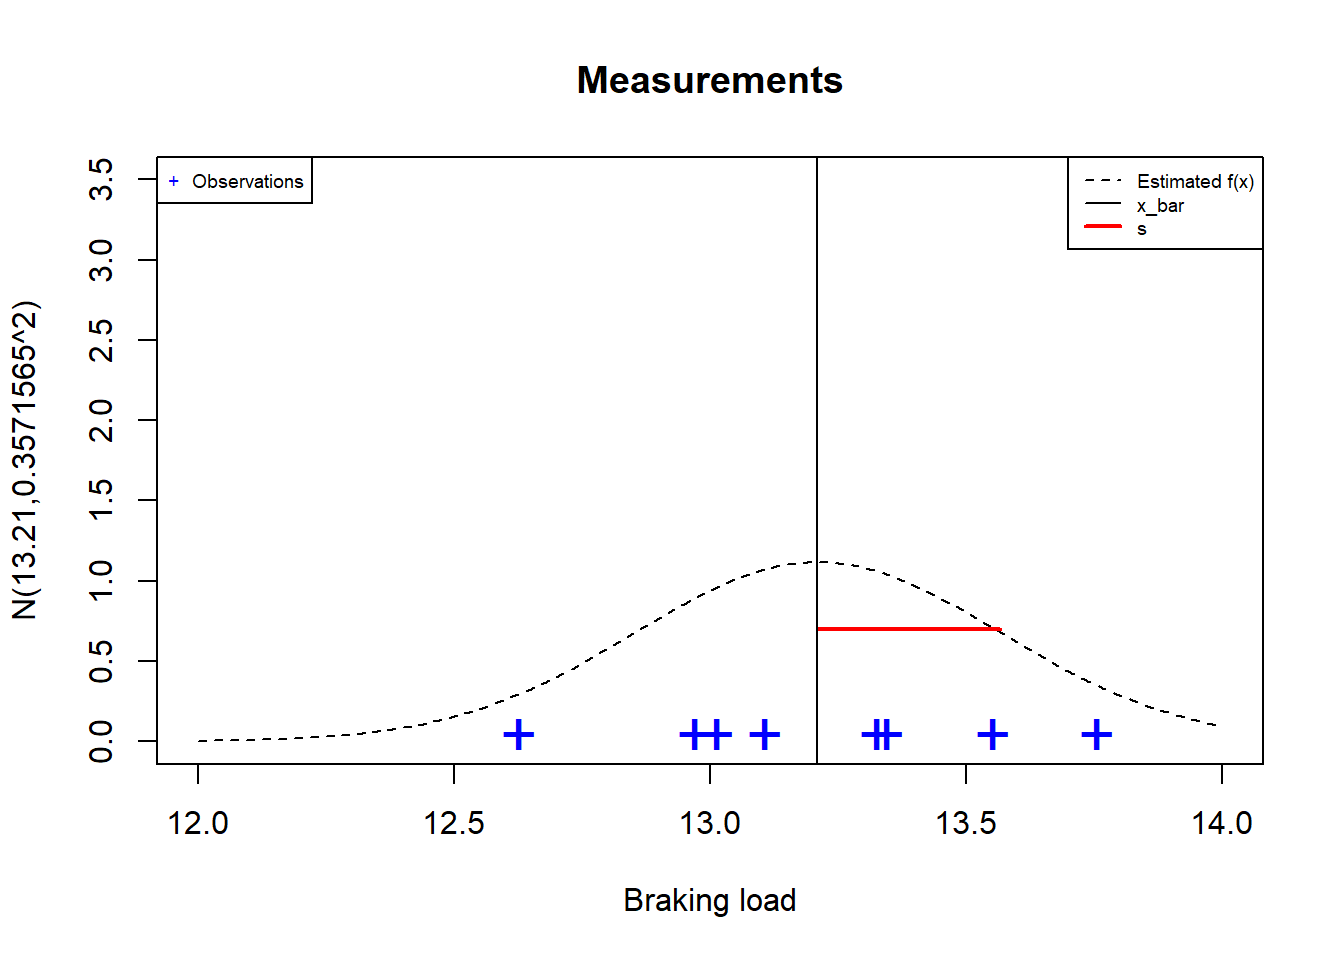
\includegraphics{_main_files/figure-latex/unnamed-chunk-71-1.pdf}

\begin{center}\rule{0.5\linewidth}{0.5pt}\end{center}

\begin{center}\rule{0.5\linewidth}{0.5pt}\end{center}

\hypertarget{ajuste-de-un-modelo}{%
\section{Ajuste de un modelo}\label{ajuste-de-un-modelo}}

\textbf{Ajustamos en un modelo} cuando

\begin{itemize}
\tightlist
\item
  \textbf{estimamos} los parámetros del modelo
\end{itemize}

También decimos que \textbf{entrenamos} un modelo (aprendizaje automático)

\textbf{Asumiendo} que

\[X \rightarrow N(x; \mu, \sigma^2)\]

Como no conocemos los parámetros, \textbf{sustituimos} las estimaciones \(\bar{x}\) y \(s^2\) como los valores de \(\mu\)
y \(\sigma^2\)

\[X \rightarrow N(x; \mu=13.21, \sigma^2=0.3571565^2)\]

\includegraphics{_main_files/figure-latex/unnamed-chunk-72-1.pdf}

\begin{center}\rule{0.5\linewidth}{0.5pt}\end{center}

\begin{center}\rule{0.5\linewidth}{0.5pt}\end{center}

\hypertarget{predicciuxf3n}{%
\section{Predicción}\label{predicciuxf3n}}

\textbf{Predecimos} el valor de un \textbf{resultado} cuando calculamos su \textbf{probabilidad}

¿Cuál es la probabilidad de que el cable se rompa a \(12\) Toneladas?

Si asumimos la variable aleatoria

\[X \rightarrow N(x; \mu, \sigma^2)\]
Sustituimos las estimaciones \(\bar{x}\) y \(s^2\) en la distribución de probabilidad

\[P(X \leq 12)= F_{normal}(12; \mu=13.21, \sigma^2=0.1275608)\]

En R pnorm(12,13.21, 0.3571565)\(=0.000352188\)

Dada la muestra \textbf{observada}, existe una probabilidad estimada de \(0.03\%\) de que un solo cable se rompa a \(12\) Toneladas.

\begin{center}\rule{0.5\linewidth}{0.5pt}\end{center}

\begin{center}\rule{0.5\linewidth}{0.5pt}\end{center}

\hypertarget{inferencia}{%
\section{Inferencia}\label{inferencia}}

Cuando tenemos una variable aleatoria normal

\[X \rightarrow N(x; \mu, \sigma^2)\]

Y conocemos \(\mu\) y \(\sigma^2\).

Podemos hacer inferencias sobre \(\bar{X}\), es decir calcular probabilidades de la variable aleatoria \(\bar{X}\).

Cuando hacemos \textbf{inferencias}, generalmente hacemos la pregunta:

¿Qué tan \textbf{seguros} estamos de que el valor del estimador \textbf{está cerca} del \textbf{parámetro verdadero}?

\begin{center}\rule{0.5\linewidth}{0.5pt}\end{center}

\begin{center}\rule{0.5\linewidth}{0.5pt}\end{center}

\hypertarget{ejemplo-cuando-suxed-conocemos-los-parametros}{%
\section{Ejemplo: Cuando sí conocemos los parametros}\label{ejemplo-cuando-suxed-conocemos-los-parametros}}

Imaginemos que nuestros cables están certificados para romper con una carga media de \(\mu = 13\) Toneladas con varianza \(\sigma^2=0.35^2\).

Tomamos una muestra aleatoria de \(8\) cables

\begin{verbatim}
## [1] 13.34642 13.32620 13.01459 13.10811 12.96999 13.55309 13.75557 12.62747
\end{verbatim}

¿Podemos afirmar que en realidad producimos cables más resistentes porque obtuvimos \(\bar{x}=13,21\) en esta muestra de \(8\) cables?

Necesitamos calcular probabilidades de \(\bar{X}\).

\begin{itemize}
\tightlist
\item
  Cuál es la probabilidad de que la distancia entre \(\bar{X}\) y \(\mu\) sea menos de \(\bar{x}_{stock}-\mu=0.21\)?
\end{itemize}

\[P(- 0.21\leq \bar{X}-\mu \leq 0.21)\]

\begin{center}\rule{0.5\linewidth}{0.5pt}\end{center}

\begin{center}\rule{0.5\linewidth}{0.5pt}\end{center}

\hypertarget{desnidad-para-x-y-para-barx}{%
\section{\texorpdfstring{Desnidad para \(X\) y para \(\bar{X}\)}{Desnidad para X y para \textbackslash bar\{X\}}}\label{desnidad-para-x-y-para-barx}}

Cuando \textbf{sabemos} que los parámetros \textbf{verdaderos} son \(\mu=13\) y \(\sigma=0.35\) esto es lo que veríamos

\includegraphics{_main_files/figure-latex/unnamed-chunk-74-1.pdf} \includegraphics{_main_files/figure-latex/unnamed-chunk-74-2.pdf}

\begin{center}\rule{0.5\linewidth}{0.5pt}\end{center}

\begin{center}\rule{0.5\linewidth}{0.5pt}\end{center}

\hypertarget{distribuciuxf3n-media-muestral}{%
\section{Distribución media muestral}\label{distribuciuxf3n-media-muestral}}

\textbf{Teorema}: Cuando \(X\) sigue una distribución normal \(X \rightarrow N(\mu, \sigma^2)\)

\(\bar{X}\) es normal:

\[\bar{X} \rightarrow N(\mu, \frac{\sigma^2}{n})\]

Entonces, si \textbf{sabemos} \(\mu\) y \(\sigma\) podemos calcular las \textbf{probabilidades de} \(\bar{X}\) usando la distribución normal.

La media y la varianza de \(\bar{X}\) son

\begin{itemize}
\tightlist
\item
  \(E(\bar{X})=\mu\)
\item
  \(V(\bar{X})=\frac{\sigma^2}{n}\)
\end{itemize}

\begin{center}\rule{0.5\linewidth}{0.5pt}\end{center}

\begin{center}\rule{0.5\linewidth}{0.5pt}\end{center}

\hypertarget{inferencia-del-promedio}{%
\section{Inferencia del promedio}\label{inferencia-del-promedio}}

\textbf{Ejemplo:}

Si \textbf{sabemos} que la rotura de nuestros cables realmente se distribuye como \[X \rightarrow N(\mu=13, \sigma^2=0.35^2)\] entonces

\[\bar{X} \rightarrow N(13, \frac{0.35^2}{8})\]

\begin{itemize}
\tightlist
\item
  \(E(\bar{X})=13\)
\item
  \(V(\bar{X})=\frac{0.35^2}{8}=0.01530169\)
\end{itemize}

Nuestro \textbf{error observado} en la estimación de la media es la diferencia

\[\bar{x}_{stock}-\mu=13.21-13=0.21\]

Nos preguntamos: ¿Es este un error \textbf{típico}?

\begin{center}\rule{0.5\linewidth}{0.5pt}\end{center}

\begin{center}\rule{0.5\linewidth}{0.5pt}\end{center}

\hypertarget{densidad-para-barx}{%
\section{\texorpdfstring{Densidad para \(\bar{X}\)}{Densidad para \textbackslash bar\{X\}}}\label{densidad-para-barx}}

Si \textbf{supiéramos} que los parámetros \textbf{verdaderos} son \(\mu=13\) y \(\sigma=0.35\) este es el error que veríamos

\includegraphics{_main_files/figure-latex/unnamed-chunk-75-1.pdf}

\begin{center}\rule{0.5\linewidth}{0.5pt}\end{center}

\begin{center}\rule{0.5\linewidth}{0.5pt}\end{center}

\hypertarget{probabilidades-de-barx}{%
\subsection{\texorpdfstring{Probabilidades de \(\bar{X}\)}{Probabilidades de \textbackslash bar\{X\}}}\label{probabilidades-de-barx}}

Si \textbf{sabemos} que la carga de rotura de nuestros cables \textbf{realmente} se distribuye como \[\bar{X} \rightarrow N(\mu=13, \frac{\sigma^2}{ n}=0.1237^2)\]

¿Cuál es la probabilidad de observar un \textbf{error de estimación} de \(\mu\) (distancia entre \(\bar{X}\) y \(\mu\)) menor a \(0.21\)?

Queremos calcular \[P(-0.21 \leq \bar{X} - 13\leq 0.21)=P(12.79 \leq \bar{X} \leq 13.21)\]

\(=F_{normal}(13,21; \mu, se^2)-F_{normal}(12,79; \mu, se^2)\)

En R podemos calcularlo como:

pnorm(13.21, 13, 0.1237)-pnorm(12.79, 13, 0.1237)=0.9104.

\(91,0\%\) de los errores son inferiores a \(0,21\), por lo que el error \textbf{observado} no parece demasiado típico (solo \(9\%\) de los errores son superiores).

Tal vez tengamos cables más fuertes de lo que pensábamos.

\begin{center}\rule{0.5\linewidth}{0.5pt}\end{center}

\begin{center}\rule{0.5\linewidth}{0.5pt}\end{center}

\hypertarget{suma-muestral}{%
\subsection{Suma muestral}\label{suma-muestral}}

Si estamos interesados en usar todos los \(8\) cables al mismo tiempo para transportar un total de \(96\) Toneladas, entonces deberíamos considerar sumar sus contribuciones individuales.

La \textbf{suma de la muestra} es la \textbf{estadística}:

\[Y=n \bar{X}=\sum_{i=1}^n X_i\]

\textbf{Teorema:} Si \(X \rightarrow N(\mu, \sigma^2)\) entonces \[Y \rightarrow N(n\mu, n\sigma^2)\]

Con media y varianza:

\begin{itemize}
\tightlist
\item
  \(E(Y)=n\mu\)
\item
  \(V(Y)=n\sigma^2\)
\end{itemize}

\begin{center}\rule{0.5\linewidth}{0.5pt}\end{center}

\begin{center}\rule{0.5\linewidth}{0.5pt}\end{center}

\hypertarget{inferencia-sobre-la-suma-muestral}{%
\subsection{Inferencia sobre la suma muestral}\label{inferencia-sobre-la-suma-muestral}}

Si \textbf{sabemos} que nuestros cables \[X \rightarrow N(\mu=13, \sigma^2=0.35^2)\] entonces

\[Y \rightarrow N(n\mu=104, n\sigma^2=8\times 0.35^2)\]

\begin{itemize}
\tightlist
\item
  \(E(Y)=104\)
\item
  \(V(Y)=8\times 0.35^2=0.98\)
\end{itemize}

Para nuestra muestra de \(8\) cables, observamos

\begin{itemize}
\tightlist
\item
  \(y_{stock}=105.7014\)
\end{itemize}

y, por tanto, el \textbf{error observado} en la estimación de la media de la \textbf{verdadera} carga de rotura total (\(n\mu\)) de \(8\) cables fue

\begin{itemize}
\tightlist
\item
  \(y_{stock}-n\mu= 1.7014\)
\end{itemize}

¿Es este un error \textbf{típico}?

\begin{center}\rule{0.5\linewidth}{0.5pt}\end{center}

\begin{center}\rule{0.5\linewidth}{0.5pt}\end{center}

\hypertarget{probabilidades-de-la-suma-muestral-propagaciuxf3n-del-error}{%
\subsection{Probabilidades de la suma muestral: Propagación del error}\label{probabilidades-de-la-suma-muestral-propagaciuxf3n-del-error}}

¿Cuál es la probabilidad de observar una diferencia \(Y-E(Y)\) menor que \(1.7014\)?

Queremos calcular la probabilidad

\[P(-1.7014 \leq \bar{Y} - 104 \leq 1.7014)=P(102.2986 \leq Y \leq 105.7014)\]

\(=F_{normal}(105.7014; n\mu, n\sigma^2)-F_{normal}(102.2986; n\mu, n\sigma^2)\)

En R podemos calcularlo como:

pnorm(105.7014, 104, sqrt(0.98)) - pnorm(102.2986, 104, sqrt(0.98))=0.914.

\(91,4\%\) de las veces tenemos sumas de cargas que son menores que \(1,7014\).

Esta proporción es mayor que la de cables individuales.

\begin{center}\rule{0.5\linewidth}{0.5pt}\end{center}

\begin{center}\rule{0.5\linewidth}{0.5pt}\end{center}

\hypertarget{inferencia-en-la-varianza-muestral}{%
\section{Inferencia en la varianza muestral}\label{inferencia-en-la-varianza-muestral}}

Consideremos un proceso de control de calidad que requiera que los cables se produzcan cerca del valor especificado \(\mu\).

Si una muestra de cables de \(8\) es muy dispersa (\(S^2>0.3\)), detenemos la producción: el proceso está fuera de control.

¿Cuál es la probabilidad de que la varianza muestral de una muestra de \(8\) cables sea mayor que los \(0,3\) requeridos?

\begin{center}\rule{0.5\linewidth}{0.5pt}\end{center}

\begin{center}\rule{0.5\linewidth}{0.5pt}\end{center}

\hypertarget{probabilidades-de-la-varianza-muestral}{%
\section{Probabilidades de la varianza muestral}\label{probabilidades-de-la-varianza-muestral}}

\textbf{Teorema:} Cuando \(X\) sigue una distribución normal
\[X \rightarrow N(\mu, \sigma^2)\]

La \textbf{estadística}:

\[W=\frac{(n-1)S^2}{\sigma^2} \rightarrow \chi^2(n-1)\]

tiene una distribución \(\chi^2\) (chi-cuadrado) con \(df=n-1\) grados de libertad dada por

\[f(w)=C_n w^{\frac{n-3}{2}} e^{-\frac{w}{2}}\]

dónde:

\begin{itemize}
\item
  \(C_n=\frac{1}{2^{(n-1)/2\sqrt{\pi(n-1)}}}\) asegura \(\int_{-\infty}^{\infty} f( t)dt=1\)
\item
  \(\Gamma(x)\) es el factorial de Euler para números reales
\item
  Si \textbf{sabemos} los valores verdaderos de \(\mu\) y \(\sigma\) podemos calcular las probabilidades de \(S^2\) usando la distribución \(\chi^2\) para \(W\).
\end{itemize}

\begin{center}\rule{0.5\linewidth}{0.5pt}\end{center}

\begin{center}\rule{0.5\linewidth}{0.5pt}\end{center}

\hypertarget{chi2-estaduxedstica}{%
\section{\texorpdfstring{\(\chi^2\)-estadística}{\textbackslash chi\^{}2-estadística}}\label{chi2-estaduxedstica}}

\includegraphics{_main_files/figure-latex/unnamed-chunk-76-1.pdf}

\begin{center}\rule{0.5\linewidth}{0.5pt}\end{center}

\begin{center}\rule{0.5\linewidth}{0.5pt}\end{center}

\hypertarget{chi2-estaduxedstica-1}{%
\section{\texorpdfstring{\(\chi^2\)-estadística}{\textbackslash chi\^{}2-estadística}}\label{chi2-estaduxedstica-1}}

Si \textbf{sabemos} que nuestros cables realmente se distribuyen como \[X \rightarrow N(\mu=13, \sigma^2=0.35^2)\]

entonces podemos calcular \[P(S^2 > 0.2)=P(\frac{(n-1)S^2}{\sigma^2} > \frac{(n-1)0.3}{\sigma^ 2})\]
\(=P(W > \frac{(n-1)0.3}{\sigma^2})\)

\(=1-P(W \leq \frac{(n-1)0.3}{\sigma^2})=1-P(W\leq \frac{(8-1)0.3}{0.1225})\)

\(= 1- F_{\chi^2,df=7}(17.14286)=0.016\)

En R
1-pchisq(17.14286, df=7)=0.016

Solo hay una probabilidad de \(1\%\) de obtener un valor superior a \(s^2=0,3\).

\begin{itemize}
\item
  \(s^2>0.3\) parece ser un buen criterio para detener la producción y revisar el proceso.
\item
  nuestro valor observado fue \(s^2_{stock}=0.1275608\)
\item
  la muestra no está demasiado dispersa y creemos que la producción está bajo control.
\end{itemize}

\hypertarget{teorema-del-luxedmite-central}{%
\chapter{teorema del límite central}\label{teorema-del-luxedmite-central}}

\hypertarget{objetivo-10}{%
\section{objetivo}\label{objetivo-10}}

\begin{itemize}
\tightlist
\item
  Margen de errores
\item
  Teorema del límite central
  -t-estadística
\end{itemize}

\begin{center}\rule{0.5\linewidth}{0.5pt}\end{center}

\begin{center}\rule{0.5\linewidth}{0.5pt}\end{center}

\hypertarget{margen-de-error}{%
\section{Margen de error}\label{margen-de-error}}

Al decidir si un \textbf{error observado} es grande o no, generalmente lo comparamos con una tolerancia \textbf{predefinida}.

\begin{itemize}
\tightlist
\item
  El \textbf{margen de error} al nivel de \(5\%\) es la distancia \(m\) tal que la distribución de \(\bar{X}\) captura \(95\%\) de las estimaciones:
\end{itemize}

\[P(-m \leq \bar{X}-\mu \leq m)=P(\mu-m \leq \bar{X} \leq\mu + m)=0.95\]

\begin{itemize}
\tightlist
\item
  o que \(95\%\) de los valores de \(\bar{X}\) están a una distancia \(m\) de \(\mu\)
\end{itemize}

\begin{center}\rule{0.5\linewidth}{0.5pt}\end{center}

\begin{center}\rule{0.5\linewidth}{0.5pt}\end{center}

\hypertarget{margen-de-error-1}{%
\section{Margen de error}\label{margen-de-error-1}}

Sigamos con el ejemplo de la carga de rotura.

para la muestra de \(8\) cables

\begin{verbatim}
## [1] 13.34642 13.32620 13.01459 13.10811 12.96999 13.55309 13.75557 12.62747
\end{verbatim}

el \textbf{error observado} es la diferencia

\[\bar{x}_{stock}-\mu=13.21-13=0.21\]
¿Está este valor por debajo del margen de error de \(5\%\)?

\begin{center}\rule{0.5\linewidth}{0.5pt}\end{center}

\begin{center}\rule{0.5\linewidth}{0.5pt}\end{center}

\hypertarget{estaduxedstica-z}{%
\section{Estadística Z}\label{estaduxedstica-z}}

Si \textbf{sabemos} que nuestros cables realmente distribuyen como
\[X \rightarrow N(\mu=13, \sigma^2=0.35^2)\] entonces,

\[\bar{X} \rightarrow N(\mu, \frac{\sigma^2}{n})\]

y el margen de error de \(5\%\) para el promedio en nuestra muestra de \(8\) cables se puede calcular a partir de la \textbf{estadística estandarizada}:

\[Z=\frac{\bar{X}-E(\bar{X})}{\sqrt{V(\bar{X})}} =\frac{\bar{X}-\mu}{ \frac{\sigma}{\sqrt{n}}} \rightarrow N(0,1)\]

\begin{center}\rule{0.5\linewidth}{0.5pt}\end{center}

\begin{center}\rule{0.5\linewidth}{0.5pt}\end{center}

\hypertarget{estaduxedstica-z-1}{%
\section{Estadística Z}\label{estaduxedstica-z-1}}

para calcular el margen de error \(m\) al nivel de \(5\%\) estandarizamos (restamos \(\mu\) y dividimos por \(\sigma/\sqrt{n}\))

\(P(\mu-m \leq \bar{X} \leq\mu + m)=P(-\frac{m}{\sigma/\sqrt{n}} \leq \frac{\bar{X} -\mu}{\frac{\sigma}{\sqrt{n}}}\leq\frac{m}{\sigma/\sqrt{n}})\)
\[=P(-\frac{m}{\sigma/\sqrt{n}} \leq Z \leq\frac{m}{\sigma/\sqrt{n}})=0,95\]

(compararlo con el gráfico) tenemos

\[m=z_{0,025} \frac{\sigma}{\sqrt{n}}=1,96\times se=1,96\frac{0,35}{\sqrt{8}}=0.24\]
donde \(z_{0.025}=1.96\) es el valor \(Z\) que deja \(2.5\%\) a cada lado de la densidad normal estándar (\(0.025\)-cuantil)

Nuestro error observado \(0.21\)

\begin{itemize}
\item
  es menor que el margen de error \(0.24\) en el nivel \(5\%\).
\item
  y, por tanto, se espera dentro de los \(95\%\) de errores.
\end{itemize}

Si una observación de \(\bar{x}\) distancia más de \(\sim 2\) veces el \(se\), decimos que el error es \textbf{inusualmente} grande.

\begin{center}\rule{0.5\linewidth}{0.5pt}\end{center}

\begin{center}\rule{0.5\linewidth}{0.5pt}\end{center}

\hypertarget{estaduxedstica-z-2}{%
\section{Estadística Z}\label{estaduxedstica-z-2}}

\textbf{Definición}

Para una variable aleatoria normal \(X\)

\[X \rightarrow N(\mu, \sigma^2)\] con \textbf{conocido} \(\sigma\)

La estadística \(Z\):

\[Z=\frac{\bar{X}-E(\bar{X})}{\sqrt{V(\bar{X})}}\]
es una variable aleatoria estándar cuyos cuantiles \(1-\alpha/2\) (\(z_{1-\alpha/2}\)) dan una medida del margen de error de \(\bar{X}\) en \(1-\alpha\) nivel

\[m=z_{1-\alpha/2}\frac{\sigma}{\sqrt{n}}\]

\textbf{Una situación común:}

\begin{itemize}
\tightlist
\item
  ¿Qué sucede cuando \(X\) no se distribuye normalmente?
\end{itemize}

\begin{center}\rule{0.5\linewidth}{0.5pt}\end{center}

\begin{center}\rule{0.5\linewidth}{0.5pt}\end{center}

\hypertarget{teorema-del-luxedmite-central-1}{%
\section{Teorema del límite central}\label{teorema-del-luxedmite-central-1}}

Para cualquier variable aleatoria \(X\) con distribución \textbf{desconocida} (de cualquier tipo)

\[X \rightarrow f(x; \theta)\]
la estadística estandarizada

\[Z=\frac{\bar{X}-E(\bar{X})}{\sqrt{V(\bar{X})}}\]

se aproxima a una distribución estándar

\[Z \rightarrow_d N(0,1)\] cuando \(n\rightarrow \infty\)

Por lo tanto:

\begin{itemize}
\tightlist
\item
  Podemos calcular probabilidades para \(\bar{X}\) si \(n\) es grande, usando la distribución normal:
\end{itemize}

\[\bar{X} \sim_{aprox} N(E(X), \frac{V(X)}{n})\]

\begin{center}\rule{0.5\linewidth}{0.5pt}\end{center}

\begin{center}\rule{0.5\linewidth}{0.5pt}\end{center}

\hypertarget{teorema-del-luxedmite-central-2}{%
\section{Teorema del límite central}\label{teorema-del-luxedmite-central-2}}

\textbf{Ejemplo:}

Consideremos un experimento en el que medimos la concentration en sangre de un fármaco después de 10 horas de administración en pacientes de \(30\). Obtenemos los siguientes resultados:

\begin{verbatim}
##  [1] 0.42172863 0.28830514 0.66452743 0.01578868 0.02810549 0.15825061
##  [7] 0.15711365 0.07263340 1.36311823 0.01457672 0.50241503 0.24010736
## [13] 0.14050681 0.18855892 0.09414202 0.42489306 0.78160177 0.23938021
## [19] 0.29546742 2.02050586 0.42157487 0.48293561 0.74263790 0.67402224
## [25] 0.58426449 0.80292617 0.74837143 0.78532627 0.01588387 0.29892485
\end{verbatim}

\begin{itemize}
\item
  el promedio es \(\bar{x}=0.56\)
\item
  el histograma de los resultados es:
\end{itemize}

\includegraphics{_main_files/figure-latex/unnamed-chunk-79-1.pdf}

\begin{center}\rule{0.5\linewidth}{0.5pt}\end{center}

\begin{center}\rule{0.5\linewidth}{0.5pt}\end{center}

\hypertarget{teorema-del-luxedmite-central-3}{%
\section{Teorema del límite central}\label{teorema-del-luxedmite-central-3}}

Si \textbf{sabemos} que los niveles siguen una distribución exponencial \[X \rightarrow exp(\lambda=2)\]

La media y la varianza son:

\begin{itemize}
\tightlist
\item
  \(E(X)=\frac{1}{\lambda}=0.5\)
\item
  \(V(X)=\frac{1}{\lambda^2}=0.25\)
\end{itemize}

Por lo tanto la media y la varianza de \(\bar{X}\) son:

\begin{itemize}
\tightlist
\item
  \(E(\bar{X})=\frac{1}{\lambda}=0.5\)
\item
  \(V(\bar{X})=\frac{V(X)}{n}=\frac{1}{n\lambda^2}=0.25/30\)
\end{itemize}

Como \(n \geq 30\)

\[Z=\frac{\bar{X}-\lambda}{\sqrt{\frac{1}{n\lambda^2}}}\]

es una variable normal estándar y: \(\bar{X} \sim_{aprox} N(\lambda, \frac{1}{n\lambda^2})\)

\begin{center}\rule{0.5\linewidth}{0.5pt}\end{center}

\begin{center}\rule{0.5\linewidth}{0.5pt}\end{center}

\includegraphics{_main_files/figure-latex/unnamed-chunk-80-1.pdf} \includegraphics{_main_files/figure-latex/unnamed-chunk-80-2.pdf}

\begin{center}\rule{0.5\linewidth}{0.5pt}\end{center}

\begin{center}\rule{0.5\linewidth}{0.5pt}\end{center}

\hypertarget{margen-de-error-con-tcl}{%
\section{Margen de error con TCL}\label{margen-de-error-con-tcl}}

Ya que

\[\bar{X} \sim_{aprox} N(E(X), \frac{V(X)}{n})\]

El margen de error en el nivel de \(5\%\)

\[P(E(X)-m \leq \bar{X} \leq E(X) + m)=0.95\]

se puede calcular de nuevo con la distribución estándar

\[m=z_{0.025} \sqrt{\frac{V(X)}{n}}=1.96\sqrt{\frac{0.25}{30}}=0.1789227\]

\textbf{Observamos} \(\bar{x}=0.5638725\) por lo tanto el \textbf{error observado} en la estimación es

\[\bar{x} - E(X)=0.5638725-0.5=0.063\]

que está dentro del margen de error.

El error que observamos es común y dentro del \(95\%\) de errores.

\begin{center}\rule{0.5\linewidth}{0.5pt}\end{center}

\begin{center}\rule{0.5\linewidth}{0.5pt}\end{center}

\hypertarget{suma-de-muestra-y-tcl}{%
\section{Suma de muestra y TCL}\label{suma-de-muestra-y-tcl}}

Para cualquier variable aleatoria \(X\) con distribución \textbf{desconocida} (cualquier tipo de)

\[X \rightarrow f(x; \theta)\]

la estadística estandarizada

\[Z=\frac{\bar{X}-E(\bar{X})}{\sqrt{V(\bar{X})}}=\frac{n\bar{X}-nE(\bar{X})}{\sqrt{nV(\bar{X})}}\]

se aproxima a una distribución estándar

\[Z \rightarrow_d N(0,1)\] cuando \(n\rightarrow \infty\)

Por lo tanto:

\begin{itemize}
\tightlist
\item
  Podemos calcular probabilidades para la suma muestral \(Y=n\bar{X}\) si \(n\) es grande, usando la distribución normal:
\end{itemize}

\[\bar{Y} \sim_{aprox} N(nE(X), nV(X))\]

\begin{center}\rule{0.5\linewidth}{0.5pt}\end{center}

\begin{center}\rule{0.5\linewidth}{0.5pt}\end{center}

\hypertarget{desconocido-sigma-pero-grande-n}{%
\section{\texorpdfstring{Desconocido \(\sigma\) pero grande \(n\)}{Desconocido \textbackslash sigma pero grande n}}\label{desconocido-sigma-pero-grande-n}}

Para cualquier variable aleatoria \(X\) con distribución \textbf{desconocida} (cualquier tipo de)

\[X \rightarrow f(x; \theta)\]

con varianza \textbf{desconocida} \(V(X)\), podemos estimar el error estándar (\(se=\sqrt{V(X)/n}\)) por la desviación estándar de la muestra

\[\hat{se}=\frac{s}{\sqrt{n}}\] y escribe la estadística estandarizada

\[Z=\frac{\bar{X}-E(\bar{X})}{\frac{s}{\sqrt{n}}} \]

\[Z \rightarrow_d N(0,1)\] para recuperar el TCL cuando \(n\rightarrow \infty\) (una buena aproximación es cuando \(n>30\))

\begin{center}\rule{0.5\linewidth}{0.5pt}\end{center}

\begin{center}\rule{0.5\linewidth}{0.5pt}\end{center}

\hypertarget{estaduxedstica-t}{%
\section{Estadística T}\label{estaduxedstica-t}}

Cuando

\begin{itemize}
\tightlist
\item
  \(\sigma\) es \textbf{desconocido}
\end{itemize}

y

\begin{itemize}
\tightlist
\item
  \(n\) es pequeño (no se puede aplicar TCL)
\end{itemize}

Sin embargo, si \(X\) es normal

\[X \rightarrow N(\mu, \sigma^2)\] entonces la estadística estandarizada

\[T=\frac{\bar{X}-\mu}{\frac{S}{\sqrt{n}}} \]

Sigue una distribución \(t\) con \(n-1\) grados de libertad, y podemos calcular probabilidades en \(\bar{X}\).

\begin{center}\rule{0.5\linewidth}{0.5pt}\end{center}

\begin{center}\rule{0.5\linewidth}{0.5pt}\end{center}

\hypertarget{estaduxedstica-t-1}{%
\section{Estadística T}\label{estaduxedstica-t-1}}

\includegraphics{_main_files/figure-latex/unnamed-chunk-81-1.pdf}

\begin{center}\rule{0.5\linewidth}{0.5pt}\end{center}

\begin{center}\rule{0.5\linewidth}{0.5pt}\end{center}

\hypertarget{estaduxedstica-t-2}{%
\section{Estadística T}\label{estaduxedstica-t-2}}

Para calcular el margen de error \(m\) a un nivel de \(5\%\) cuando \(n\) es pequeño, \(\sigma\) desconocido pero \(X\) normal

\(P(\mu-m \leq \bar{X} \leq\mu + m)=P(-\frac{m}{s/\sqrt{n}} \leq \frac{\bar{X}- \mu}{\frac{s}{\sqrt{n}}} \leq\frac{m}{s/\sqrt{n}})\)
\[=P(-\frac{m}{s/\sqrt{n}} \leq T \leq\frac{m}{s/\sqrt{n}})=0,95\]

Usamos la distribución \(t\)

\[m=t_{0.025, n-1} \frac{s}{\sqrt{n}}\]
donde \(t_{0.025, n-1}\) es el valor \(T\) que deja \(2.5\%\) a cada lado de la distribución \(t\) con \(n-1\) grados de libertad (\(0.025\)-cuantil)

\begin{center}\rule{0.5\linewidth}{0.5pt}\end{center}

\begin{center}\rule{0.5\linewidth}{0.5pt}\end{center}

\hypertarget{ejemplo-1-3}{%
\section{Ejemplo 1}\label{ejemplo-1-3}}

Volviendo al ejemplo de la carga de rotura, calculamos el margen de error con \textbf{conocido} \(\sigma^2=0.35^2\).

\[m=z_{0,025} \frac{\sigma}{\sqrt{n}}=1,96\times se=1,96\frac{0,35}{\sqrt{8}}=0,24\]

\begin{itemize}
\tightlist
\item
  En la mayoría de las aplicaciones \textbf{no conocemos} los parámetros
\end{itemize}

Si solo asumiéramos que la carga de rotura es una variable aleatoria normal

\[X \rightarrow N(\mu, \sigma^2)\]
con \textbf{desconocido} \(\mu\) y \(\sigma^2\) luego de los datos

\begin{itemize}
\tightlist
\item
  \(s_{stock}=\sqrt{0.1275608}\)
\end{itemize}

y el margen de error es \[m=t_{0.025, n-1} \frac{s}{\sqrt{n}}=2.36\times \hat{se}=2.36\frac{0.3571565}{\sqrt{ 8}}=0.29\]
donde \(t_{0.025, n-1}=2.36\)

en R es qt(1-0.025, 7)

Aumentó a partir del valor que obtuvimos con \textbf{conocido} \(\sigma\)

\begin{center}\rule{0.5\linewidth}{0.5pt}\end{center}

\begin{center}\rule{0.5\linewidth}{0.5pt}\end{center}

\hypertarget{ejemplo-2-2}{%
\section{Ejemplo 2}\label{ejemplo-2-2}}

También podemos preguntar por la probabilidad de observar un error en la estimación de \(\mu\) (distancia entre \(\bar{X}\) y \(\mu\)) menor que el valor observado \(0.21\)?

Entonces queremos calcular \[P(-0.21 \leq \bar{X} - \mu\leq 0.21)=P(\frac{-0.21}{s/\sqrt{n}} \leq T \leq \frac {0.21}{s/\sqrt{n}})\]

\(=P(\frac{-0.21}{0.3571565/\sqrt{8}} \leq T \leq \frac{0.21}{0.3571565/\sqrt{8}})\)

\(=F_{t, n-1}(0,21)-F_{t, n-1}(-0,21)\)

En R podemos calcularlo como:

pt(1.663052, 7)-pt(-1.663052, 7)=0.859.

\(85,9\%\) de los errores son inferiores a \(0,21\), por lo que el error \textbf{observado} parece más típico que el \(91\%\) que obtenemos con \(\sigma^2=0,35^2\).

Tenga en cuenta que en los cálculos hemos sustituido \(\sigma=0.35\) por una estimación más alta \(s=0.3571565\) \textbf{obtenida de los datos}.

\hypertarget{ejercicios}{%
\chapter{Ejercicios}\label{ejercicios}}

\hypertarget{descripciuxf3n-de-datos-1}{%
\section{Descripción de datos}\label{descripciuxf3n-de-datos-1}}

\hypertarget{ejercicio-1}{%
\subsubsection{Ejercicio 1}\label{ejercicio-1}}

Hemos realizado un experimento 12 veces con los siguientes resultados

\begin{verbatim}
## [1]  3  3 10  2  6 11  5  4
\end{verbatim}

Responde las siguientes preguntas:

\begin{itemize}
\tightlist
\item
  Calcula las frecuencias relativas de cada resultado.
\item
  Calcula las frecuencias acumuladas de cada resultado.
\item
  ¿Cuál es el promedio de las observaciones?
\item
  ¿Qué es la mediana?
\item
  ¿Qué es el tercer cuartil?
\item
  ¿Cuál es el primer cuartil?
\end{itemize}

\hypertarget{ejercicio-2}{%
\subsubsection{Ejercicio 2}\label{ejercicio-2}}

Hemos realizado un experimento 10 veces con los siguientes resultados

\begin{verbatim}
##  [1] 2.875775 7.883051 4.089769 8.830174 9.404673 0.455565 5.281055 8.924190
##  [9] 5.514350 4.566147
\end{verbatim}

Considere 10 contenedores de tamaño 1: {[}0,1{]}, (1,2{]}\ldots(9,10).

Responde las siguientes preguntas:

\begin{itemize}
\item
  Calcula las frecuencias relativas de cada resultado y dibuje el histograma
\item
  Calcula las frecuencias acumulativas de cada resultado y dibuje la gráfica acumulativa.
\item
  Dibuja un diagrama de caja.
\end{itemize}

\hypertarget{probabilidad-3}{%
\section{Probabilidad}\label{probabilidad-3}}

\hypertarget{ejercicio-1-1}{%
\subsubsection{Ejercicio 1}\label{ejercicio-1-1}}

El resultado de un experimento aleatorio es medir la gravedad de la misofonía \textbf{y} el estado de depresión de un paciente.

\begin{itemize}
\tightlist
\item
  Gravedad de la misofonía: \(x\in \{0,1,2,3,4\}\)
\item
  Depresión: \(y\in \{0,1\}\) (no:\(0\), si:\(1\))
\end{itemize}

\begin{verbatim}
##   Misofonia.dic depresion.dic
## 1             4             1
## 2             2             0
## 3             0             0
## 4             3             0
## 5             0             0
## 6             0             0
\end{verbatim}

Un estudio en 123 pacientes mostró las frecuencias \(n_{x,y}\) dadas en la tabla de contingencia:

\begin{verbatim}
##               
##                Depression:0 Depression:1
##   Misophonia:4            0            9
##   Misophonia:3           25            6
##   Misophonia:2           34            3
##   Misophonia:1            5            0
##   Misophonia:0           36            5
\end{verbatim}

Supongamos que \(N>>0\) y que las frecuencias \textbf{estiman} las probabilidades \(f_{x,y}=\hat{P}(X, Y)\)

\begin{verbatim}
##               
##                Depression:0 Depression:1
##   Misophonia:4   0.00000000   0.07317073
##   Misophonia:3   0.20325203   0.04878049
##   Misophonia:2   0.27642276   0.02439024
##   Misophonia:1   0.04065041   0.00000000
##   Misophonia:0   0.29268293   0.04065041
\end{verbatim}

\begin{itemize}
\tightlist
\item
  ¿Cuál es la probabilidad marginal de misofonía de gravedad 3?(R/0.3)
\item
  ¿Cuál es la probabilidad de no ser misofónico \textbf{y} no estar deprimido?(R/0.293)
\item
  ¿Cuál es la probabilidad de ser misofónico \textbf{o} deprimido?(R/0.293)
\item
  ¿Cuál es la probabilidad de ser misofónico \textbf{y} deprimido?(R/0.707)
\item
  Describir en palabras los resultados con probabilidad 0.
\end{itemize}

\hypertarget{ejercicio-2-1}{%
\subsubsection{Ejercicio 2}\label{ejercicio-2-1}}

Hemos realizado un experimento 10 veces con los siguientes resultados

\begin{verbatim}
##         A     B
## 1    male  dead
## 2    male  dead
## 3    male  dead
## 4  female alive
## 5    male  dead
## 6  female alive
## 7  female  dead
## 8  female alive
## 9    male alive
## 10   male alive
\end{verbatim}

\begin{itemize}
\tightlist
\item
  Crear la tabla de contingencia para el número (\(n_{i,j}\)) de observaciones de cada resultado (\(A,B\))
\item
  Crear la tabla de contingencia para la frecuencia relativa (\(f_{i,j}\)) de los resultados
\item
  ¿Cuál es la frecuencia marginal de ser hombre? (R/0.6)
\item
  ¿Cuál es la frecuencia marginal de estar vivo? (R/0.5)
\item
  ¿Cuál es la frecuencia de estar vivo \textbf{o} mujer? (R/0.6)
\end{itemize}

\hypertarget{la-probabilidad-condicional-2}{%
\section{La probabilidad condicional}\label{la-probabilidad-condicional-2}}

\hypertarget{ejercicio-1-2}{%
\subsubsection{Ejercicio 1}\label{ejercicio-1-2}}

Se prueba el rendimiento de una máquina para producir varillas de torneado de alta calidad. Estos son los resultados de las pruebas

\begin{longtable}[]{@{}ccc@{}}
\toprule
& Redondeado: Sí & Redondeado: No \\
\midrule
\endhead
superficie lisa: sí & 200 & 1 \\
superficie lisa: no & 4 & 2 \\
\bottomrule
\end{longtable}

\begin{itemize}
\item
  ¿Cuál es la probabilidad estimada de que la máquina produzca una varilla que no satisfaga ningún control de calidad? (R: 2/207)
\item
  ¿Cuál es la probabilidad estimada de que la máquina produzca una varilla que no satisfaga al menos un control de calidad? (R: 7/207)
\item
  ¿Cuál es la probabilidad estimada de que la máquina produzca varillas de superficie redondeada y alisada? (R: 200/207)
\item
  ¿Cuál es la probabilidad estimada de que la barra sea redondeada si la barra es lisa? (R: 201/201)
\item
  ¿Cuál es la probabilidad estimada de que la varilla sea lisa si es redondeada? (R: 201/204)
\item
  ¿Cuál es la probabilidad estimada de que la varilla no sea ni lisa ni redondeada si no cumple al menos un control de calidad? (R: 2/7)
\item
  ¿Son eventos independientes la suavidad y la redondez? (no)
\end{itemize}

\hypertarget{ejercicio-2-2}{%
\subsubsection{Ejercicio 2}\label{ejercicio-2-2}}

Desarrollamos un test para detectar la presencia de bacterias en un lago. Encontramos que si el lago contiene la bacteria, la prueba es positiva el 70\% de las veces. Si no hay bacterias, la prueba es negativa el 60\% de las veces. Implementamos la prueba en una región donde sabemos que el 20\% de los lagos tienen bacterias.

\begin{itemize}
\tightlist
\item
  ¿Cuál es la probabilidad de que un lago que dé positivo esté contaminado con bacterias? (R: 0.30)
\end{itemize}

\hypertarget{ejercicio-3}{%
\subsubsection{Ejercicio 3}\label{ejercicio-3}}

Se prueba el rendimiento de dos máquinas para producir varillas de torneado de alta calidad. Estos son los resultados de las pruebas

\textbf{Máquina 1}

\begin{longtable}[]{@{}ccc@{}}
\toprule
& Redondeado: Sí & Redondeado: No \\
\midrule
\endhead
superficie lisa: sí & 200 & 1 \\
superficie lisa: no & 4 & 2 \\
\bottomrule
\end{longtable}

\textbf{Máquina 2}

\begin{longtable}[]{@{}ccc@{}}
\toprule
& Redondeado: Sí & Redondeado: No \\
\midrule
\endhead
superficie lisa: sí & 145 & 4 \\
superficie lisa: no & 8 & 6 \\
\bottomrule
\end{longtable}

\begin{itemize}
\tightlist
\item
  ¿Cuál es la probabilidad de que la barra sea redondeada? (R: 357/370)
\item
  ¿Cuál es la probabilidad de que la varilla haya sido producida por la máquina 1? (R: 207/370)
\item
  ¿Cuál es la probabilidad de que la varilla no sea lisa? (R: 20/370)
\item
  ¿Cuál es la probabilidad de que la varilla sea lisa o redondeada o producida por la máquina 1? (R: 364/370)
\item
  ¿Cuál es la probabilidad de que la varilla quede redondeada si es alisada y de la máquina 1? (R: 200/201)
\item
  ¿Cuál es la probabilidad de que la varilla no esté redondeada si no está alisada y es de la máquina 2? (R: 6/8)
\item
  ¿Cuál es la probabilidad de que la varilla haya salido de la máquina 1 si está alisada y redondeada? (R: 200/345)
\item
  ¿Cuál es la probabilidad de que la varilla haya venido de la máquina 2 si no pasa al menos uno de los controles de calidad? (R:0.72)
\end{itemize}

\hypertarget{ejercicio-4}{%
\subsubsection{Ejercicio 4}\label{ejercicio-4}}

Queremos cruzar una avenida con dos semáforos. La probabilidad de encontrar el primer semáforo en rojo es 0,6. Si paramos en el primer semáforo, la probabilidad de parar en el segundo es 0,15. Mientras que la probabilidad de detenernos en el segundo si no nos detenemos en el primero es 0,25.

Cuando intentamos cruzar ambos semáforos:

\begin{itemize}
\tightlist
\item
  ¿Cuál es la probabilidad de tener que detenerse en cada semáforo? (R:0.09)
\item
  ¿Cuál es la probabilidad de tener que parar en al menos un semáforo? (R:0.7)
\item
  ¿Cuál es la probabilidad de tener que detenerse en un solo semáforo? (R:0.61)
\item
  Si paré en el segundo semáforo, ¿cuál es la probabilidad de que hubiera tenido que parar en el primero? (R: 0.62)
\item
  Si tuviera que parar en cualquier semáforo, ¿cuál es la probabilidad de que tuviera que hacerlo dos veces? (R: 0.12)
\item
  ¿Parar en el primer semáforo es un evento independiente de detenerse en el segundo semáforo? (no)
\end{itemize}

Ahora, queremos cruzar una avenida con tres semáforos. La probabilidad de encontrar un semáforo en rojo solo depende de la anterior. En concreto, la probabilidad de encontrar un semáforo en rojo dado que el anterior estaba en rojo es de 0,15. Mientras que la probabilidad de encontrar un tráfico justo en rojo dado que el anterior estaba en verde es de 0,25. Además, la probabilidad de encontrar el primer semáforo en rojo es de 0,6.

\begin{itemize}
\tightlist
\item
  ¿Cuál es la probabilidad de tener que parar en cada semáforo? (R:0.013)
\item
  ¿Cuál es la probabilidad de tener que parar en al menos un semáforo? (R:0.775)
\item
  ¿Cuál es la probabilidad de tener que detenerse en un solo semáforo? (R:0.5425)
\end{itemize}

consejos:

\begin{itemize}
\item
  Si la probabilidad de que un semáforo esté en rojo depende únicamente del anterior, entonces
  \(P(R_3|R_2,R_1)=P(R_3|R_2,\bar{R}_1)=P(R_3|R_2)\) y \(P(R_3|\bar{R}_2,R_1)=P(R_3 |\bar{R}_2,\bar{R}_1)=P(R_3|\bar{R}_2)\)
\item
  La probabilidad conjunta de encontrar tres semáforos en rojo se puede escribir como:
  \(P(R_1,R_2,R_3)=P(R_3|R_2)P(R_2|R_1)P(R_1)\)
\end{itemize}

\hypertarget{ejercicio-5}{%
\subsubsection{Ejercicio 5}\label{ejercicio-5}}

Una prueba de calidad en un ladrillo aleatorio se define por los eventos:

\begin{itemize}
\tightlist
\item
  Pasar la prueba de calidad: \(E\), no pasar la prueba de calidad: \(\bar{E}\)
\item
  Defectuoso: \(D\), no defectuoso: \(\bar{D}\)
\end{itemize}

Si la prueba diagnóstica tiene sensibilidad \(P(E|\bar{D})=0.99\) y especificidad \(P(\bar{E}|D)=0.98\), y la probabilidad de pasar la prueba es \(P(E) =0.893\) entonces

\begin{itemize}
\item
  ¿Cuál es la probabilidad de que un ladrillo elegido al azar sea defectuoso \(P(D)\)? (R:0.1)
\item
  ¿Cuál es la probabilidad de que un ladrillo que ha pasado la prueba sea realmente defectuoso? (R:0.022)
\item
  La probabilidad de que un ladrillo no sea defectuoso \textbf{y} que no pase la prueba (R:0.009)
\item
  ¿Son \(D\) y \(\bar{E}\) estadísticamente independientes? (no)
\end{itemize}

\hypertarget{variables-aleatorias}{%
\section{Variables aleatorias}\label{variables-aleatorias}}

\hypertarget{ejercicio-1-3}{%
\subsubsection{Ejercicio 1}\label{ejercicio-1-3}}

Dada la función de masa de probabilidad

\begin{longtable}[]{@{}cc@{}}
\toprule
\(x\) & \(f(x)=P(X=x)\) \\
\midrule
\endhead
10 & 0.1 \\
12 & 0.3 \\
14 & 0.25 \\
15 & 0.15 \\
17 & ? \\
20 & 0.15 \\
\bottomrule
\end{longtable}

\begin{itemize}
\tightlist
\item
  ¿Cuál es su valor esperado y su desviación estándar? (R: 14.2; 2.95)
\end{itemize}

\hypertarget{ejercicio-2-3}{%
\subsubsection{Ejercicio 2}\label{ejercicio-2-3}}

Dada la distribución de probabilidad para una variable discreta \(X\)

\[
    F(x)=
\begin{cases}
0, & x < -1 \\
0.2,& x \in [-1,0)\\
0.35,& x \in [0,1)\\
0.45,& x \in [1,2)\\
1,& x \geq 2\\
\end{cases}
\]

\begin{itemize}
\tightlist
\item
  encuentra \(f(X)\)
\item
  encuentra \(E(X)\) y \(V(X)\) (R:1; 1.5)
\item
  cuál es el valor esperado y la varianza de \(Y=2X+3\) (R: 6)
\item
  ¿Cuál es la mediana y el primer y tercer cuartil de \(X\)? (R:2,0,2)
\end{itemize}

\hypertarget{ejercicio-3-1}{%
\subsubsection{Ejercicio 3}\label{ejercicio-3-1}}

Estamos probando un sistema para transmitir imágenes digitales. Primero consideramos el experimento de enviar \(3\) píxeles y tener por ejemplo eventos como \((0,1,1)\). Este es el evento de recibir el primer píxel sin error, el segundo con error y el tercero con error.

\begin{itemize}
\item
  Enumere en una columna el espacio muestral del experimento aleatorio.
\item
  En la segunda columna asigne la variable aleatoria que cuenta el número de errores transmitidos para cada resultado
\end{itemize}

Considere que tenemos un canal totalmente ruidoso, es decir, cualquier resultado de tres píxeles es igualmente probable.

\begin{itemize}
\item
  ¿Cuál es la probabilidad de recibir errores de \(0\), \(1\), \(2\) o \(3\) en la transmisión de \(3\) píxeles? (R: 1/8; 3/8; 3/8; 1/8)
\item
  Dibuje la función de masa de probabilidad para el número de errores
\item
  ¿Cuál es el valor esperado para el número de errores? (R:1.5)
\item
  ¿Cuál es su varianza? (R: 0.75)
\item
  Dibujar la distribución de probabilidad
\item
  ¿Cuál es la probabilidad de transmitir al menos \(1\) error?
  (R:7/8)
\end{itemize}

\hypertarget{ejercicio-4-1}{%
\subsubsection{Ejercicio 4}\label{ejercicio-4-1}}

Para la densidad de probabilidad

\[
    f(x)=
\begin{cases}
    \frac{1}{100},& \text{si } x\in (0,100)\\
    0, de\, lo\, contrario
\end{cases}
\]

\begin{itemize}
\tightlist
\item
  calcular la media (R:50)
\item
  calcular la varianza usando \(E(X^2)=V(X)+E(X)^2\) (R:100\^{}2/12)
\item
  calcular \(P(\mu-\sigma\leq X \leq \mu+\sigma)\)(R: 0.57)
\item
  ¿Cuáles son el primer y tercer cuartiles? (R: 25; 75)
\end{itemize}

\includegraphics{_main_files/figure-latex/unnamed-chunk-88-1.pdf}

\hypertarget{ejercicio-5-1}{%
\subsubsection{Ejercicio 5}\label{ejercicio-5-1}}

Dado
\[
    f(x)= 
\begin{cases}
0, & x < 0 \\
ax, & x \in [0,3] \\
b, & x \in (3,5) \\
\frac{b}{3}(8-x),& x \in [5,8]\\
0, & x > 8 \\
\end{cases}
\]

\begin{itemize}
\item
  ¿Cuáles son los valores de \(a\) y \(b\) tales que \(f(x)\) es una función de densidad de probabilidad continua? (R: 1/15; 1/5)
\item
  ¿Cuál es la media de \(X\)? (R:4)
\end{itemize}

\hypertarget{ejercicio-6}{%
\subsubsection{Ejercicio 6}\label{ejercicio-6}}

Para la densidad de probabilidad

\[
    f(x)= 
\begin{cases}
    \lambda e^{-\lambda x},& \text{if } x \geq 0\\
    0,& si\,no 
\end{cases}
\]

\begin{itemize}
\tightlist
\item
  Confirmar que se trata de una densidad de probabilidad
\item
  Calcular la media (R: 1/\(\lambda\))
\item
  Calcule el valor esperado de \(X^2\) (R: 2/\(\lambda^2\))
\item
  Calcular la varianza (R: 1/\(\lambda^2\))
\item
  Hallar la distribución de probabilidad \(F(a)\) (R: \(1-exp(-\lambda a)\))
\item
  Encuentra la mediana (R: \(\log{2}\)/\(\lambda\))
\end{itemize}

\hypertarget{ejercicio-7}{%
\subsubsection{Ejercicio 7}\label{ejercicio-7}}

Dada la distribución de probabilidad de una variable aleatoria \(X\)

\[
    F(x)= 
\begin{cases}
0, & x  < -1 \\
\frac{1}{80}(17+16x-x^2),& x \in [-1,7)\\
1,& x \geq 7\\
\end{cases}
\]

calcular:

\begin{itemize}
\tightlist
\item
  \(P(X>0)\) (R:63/80)
\item
  \(E(X)\) (R:1.93)
\item
  \(P(X>0|X<2)\) (R:28/45)
\end{itemize}

\hypertarget{modelos-de-probabilidad}{%
\section{Modelos de probabilidad}\label{modelos-de-probabilidad}}

\hypertarget{ejercicio-1-4}{%
\subsubsection{Ejercicio 1}\label{ejercicio-1-4}}

En una población, la probabilidad de que nazca un niño es \(p=0.51\). Considere una familia de \(4\) hijos.

\begin{itemize}
\tightlist
\item
  ¿Cuál es la probabilidad de que una familia de 4 hijos tenga un solo niño? (R: 0.240)
\item
  ¿Cuál es la probabilidad de que una familia tenga una sola niña? (R: 0.259)
\item
  ¿Cuál es la probabilidad de que una familia tenga o solo un niño o solo una niña?(R: 0.4999)
\item
  ¿Cuál es la probabilidad de que la familia tenga al menos dos niños? (R: 0.7023)
\item
  ¿Cuál es el número de hijos que debe tener una familia para que la probabilidad de tener al menos una niña sea superior a \(0.75\)? (R:\(n=3>\log(0.25)/\log(0.51)\))
\end{itemize}

\hypertarget{ejercicio-2-4}{%
\subsubsection{Ejercicio 2}\label{ejercicio-2-4}}

Un motor de búsqueda falla al recibir una petición con una probabilidad de \(0.1\)

\begin{itemize}
\item
  Si nuestro sistema recibe \(50\) solicitudes de búsqueda, ¿cuál es la probabilidad de que el sistema no responda a tres de ellas? (R:0.1385651)
\item
  ¿Cuál es la probabilidad de que el motor complete con éxito \(15\) búsquedas antes del primer fallo? (R:0.020)
\item
  Consideramos que un buscador funciona suficientemente bien cuando es capaz de encontrar información para mas de \(10\) solicitudes por cada \(2\) fallos. ¿Cuál es la probabilidad de que en un ensayo de fiabilidad nuestro motor de búsqueda sea satisfactorio?
  (R: 0.697)
\end{itemize}

\hypertarget{ejercicio-3-2}{%
\subsubsection{Ejercicio 3}\label{ejercicio-3-2}}

La cantidad promedio de partículas radiactivas que golpean un contador Geiger en una planta de energía nuclear bajo control es de \(2.3\) por minuto.

\begin{itemize}
\item
  ¿Cuál es la probabilidad de contar exactamente \(2\) partículas en un minuto? (R:0.265)
\item
  ¿Cuál es la probabilidad de detectar exactamente \(10\) partículas en \(5\) minutos? (R:0.112)
\item
  ¿Cuál es la probabilidad de observar al menos una partículas en dos minutos? (R:0.953)
\item
  ¿Cuál es la probabilidad de tener que esperar menos de \(1\) segundo para detectar una partícula radiactiva, después de encender el detector? (R:0.037)
\item
  Sospechamos que una planta nuclear tiene una fuga radiactiva si esperamos menos de \(1\) segundo para detectar una partícula radiactiva, después de encender el detector. ¿Cuál es la probabilidad de que cuando visitemos \(5\) plantas que están bajo control, sospechemos que al menos una tiene una fuga? (R:0.1744).
\end{itemize}

\hypertarget{ejercicio-4-2}{%
\subsubsection{Ejercicio 4}\label{ejercicio-4-2}}

\begin{itemize}
\item
  ¿Cuál es la probabilidad de que la altura de un hombre sea al menos
  \(165\)cm si la media poblacional es \(175\)cm y la desviación estándar es \(10\)cm? (R:0.841)
\item
  ¿Cuál es la probabilidad de que la altura de un hombre esté entre
  \(165\)cm y \(185\)cm? (R:0.682)
\item
  ¿Cuál es la altura que define el \(5\%\) de los hombres más pequeños? (R:158.55)
\end{itemize}

\hypertarget{muestreo-y-teorema-del-luxedmite-central}{%
\section{Muestreo y teorema del límite central}\label{muestreo-y-teorema-del-luxedmite-central}}

\hypertarget{ejercicio-1-5}{%
\subsubsection{Ejercicio 1}\label{ejercicio-1-5}}

Un tipo de batería carga hasta el \(75\%\) de su capacidad en una hora, con una desviación estándar de \(15\%\).

\begin{itemize}
\item
  Si cargamos \(25\) baterias, ¿cuál es la probabilidad de que la diferencia de carga entre el promedio de la muestra y la media sea como máximo de un \(5\%\)? (R:0.9044)
\item
  Si cargamos \(100\) baterías, ¿cuál es esa probabilidad? (R:0.9991)
\item
  Si, en cambio, solo cargamos \(9\) baterías, ¿cuál valor \(c\) que es superado por la media muestral con una probabilidad del \(0.015\)? (R:85.850)
\end{itemize}

\hypertarget{ejercicio-2-5}{%
\subsubsection{Ejercicio 2}\label{ejercicio-2-5}}

Se necesita un componente electrónico para el correcto funcionamiento de un telescopio. Necesita ser reemplazado inmediatamente cuando se desgasta.

La vida media del componente (\(\mu\)) es de \(100\) horas y su desviación estándar \(\sigma\) es de \(30\) horas.

\begin{itemize}
\item
  ¿Cuál es la probabilidad de que el promedio de la vida media de \(50\) componentes esté dentro de \(1\) hora de la vida media de un solo componente? (R:0.1863)
\item
  ¿Cuántos componentes necesitamos para que el telescopio esté operativo \(2750\) horas consecutivas con una probabilidad de por lo menos \(0,95\)? (R:31)
\end{itemize}

\hypertarget{ejercicio-3-3}{%
\subsubsection{Ejercicio 3}\label{ejercicio-3-3}}

Una máquina automática llena tubos de ensayo con muestras biológicas con una media de \(\mu=130\)mg y una desviación estándar de \(\sigma=5\)mg.

\begin{itemize}
\item
  para una muestra aleatoria de tamaño \(50\). ¿Cuál es la probabilidad de que
  la media muestral (promedio) está entre \(128\) y \(132\)gr?
\item
  ¿Cuál debe ser el tamaño de la muestra (\(n\)) para que la media muestral \(\bar{X}\) sea mayor a \(131\)gr con una probabilidad menor o igual a \(0.025\)?
\end{itemize}

\hypertarget{ejercicio-4-3}{%
\subsubsection{Ejercicio 4}\label{ejercicio-4-3}}

En el Caribe, parece haber un promedio de huracanes de \(6\) por año. Teniendo en cuenta que la formación de huracanes es un proceso de Poisson, los meteorólogos planean estimar el tiempo medio entre la formación de dos huracanes. Planean recolectar una muestra de tamaño \(36\) para los tiempos entre dos huracanes.

\begin{itemize}
\item
  ¿Cuál es la probabilidad de que su promedio muestral esté entre \(45\) y \(60\) días?
\item
  ¿Cuál debe ser el tamaño de la muestra para que tengan una probabilidad de \(0.025\) de que la media muestral sea mayor a \(70\) días?
\end{itemize}

\hypertarget{ejercicio-5-2}{%
\subsubsection{Ejercicio 5}\label{ejercicio-5-2}}

La probabilidad de que se encuentre una mutación particular en la población es de \(0.4\). Si probamos \(2000\) personas para la mutación:

\begin{itemize}
\tightlist
\item
  ¿Cuál es la probabilidad de que el número total de personas con la mutación esté entre \(791\) y \(809\)?
\end{itemize}

sugerencia: use el CLT con una muestra de ensayos de Bernoulli de \(2000\). Esto se conoce como la aproximación normal de la distribución binomial.

\hypertarget{estimadores-puntuales}{%
\section{Estimadores puntuales}\label{estimadores-puntuales}}

\hypertarget{ejercicio-1-6}{%
\subsubsection{Ejercicio 1}\label{ejercicio-1-6}}

Considere el modelo de probabilidad

\[
    f(x)= 
\begin{cases}
    1/2-a,& \text{si } x=-1 \\ 
    1/2,& \text{si } x=0\\
    a,& 1 \text{si } x=1\\ 
\end{cases}
\]

donde \(a\) es un parámetro.

Calcule la media y la varianza de la estadística: \[T=\frac{\bar{X}}{2}+\frac{1}{4}\]

donde \(\bar{X}=\frac{1}{N}\sum_{i=1}^N X_i\)

\begin{itemize}
\item
  ¿\(T\) es un estimador sesgado de \(a\)?
\item
  ¿Es \(T\) consistente? es decir, \(V(T) \rightarrow 0\) cuando \(N\rightarrow \infty\)
\end{itemize}

\hypertarget{ejercicio-2-6}{%
\subsubsection{Ejercicio 2}\label{ejercicio-2-6}}

\begin{itemize}
\tightlist
\item
  ¿Es \(\bar{X}^2=(\frac{1}{N}\sum_{i=1}^N X_i)^2\) un estimador imparcial de \(E(X)^2\)?
\end{itemize}

\hypertarget{muxe1xima-verosimilitud}{%
\section{Máxima verosimilitud}\label{muxe1xima-verosimilitud}}

\hypertarget{ejercicio-1-7}{%
\subsubsection{Ejercicio 1}\label{ejercicio-1-7}}

Para una variable aleatoria con una función de probabilidad binomial

\[f(x; p)=\binom n x p^x(1-p)^{n-x}\]

\begin{itemize}
\item
  ¿Cuál es el estimador de máxima verosimilitud de \(p\) para una muestra de tamaño \(1\) de esta variable aleatoria?
\item
  En \textbf{un} examen de \(100\) estudiantes observamos \(x_1=68\) estudiantes que aprobaron el examen. ¿Cuál es la estimación de \(p\)?
\end{itemize}

\hypertarget{ejercicio-2-7}{%
\subsubsection{Ejercicio 2}\label{ejercicio-2-7}}

Tome una variable aleatoria con la siguiente función de densidad de probabilidad

\[
f(x)=
\begin{cases}
    (1+\theta)x^\theta,& \text{si } x\in (0,1)\\
    0,&  x\notin (0,1)
\end{cases}
\]

\begin{itemize}
\item
  ¿Cuál es la estimación de máxima verosimilitud para \(\theta\)?
\item
  Si tomamos una muestra de \(5\) con observaciones
  \(x_1 = 0,92; \qquad x_2 = 0,79; \qquad x_3 = 0,90; \qquad x_4 = 0,65; \qquad x_5 = 0,86\)
\end{itemize}

¿Cuál es el valor estimado del parámetro \(\theta\)?

\hypertarget{ejercicio-3-4}{%
\subsubsection{Ejercicio 3}\label{ejercicio-3-4}}

Tome una variable aleatoria con la siguiente función de densidad de probabilidad

\[
    f(x)= 
\begin{cases}
    \lambda e^{-\lambda x},& \text{si } 0 \leq x\\
    0,& si \, no 
\end{cases}
\]

\begin{itemize}
\item
  ¿Cuál es la estimación de máxima verosimilitud para \(\lambda\)?
\item
  Si tomamos una muestra de \(5\) con observaciones
  \(x_1 = 0.223 \qquad x_2 = 0.681; \qquad x_3 = 0,117; \qquad x_4 = 0,150; \qquad x_5 = 0.520\)
\end{itemize}

¿Cuál es el valor estimado del parámetro \(\lambda\)?

\hypertarget{muxe9todo-de-los-momentos}{%
\section{Método de los momentos}\label{muxe9todo-de-los-momentos}}

\hypertarget{ejercicio-1-8}{%
\subsubsection{Ejercicio 1}\label{ejercicio-1-8}}

¿Cuáles son los estimadores de los siguientes modelos paramétricos dados por el método de los momentos?

\begin{longtable}[]{@{}lll@{}}
\toprule
modelo & f(x) & E(X) \\
\midrule
\endhead
Bernoulli & \(p^x(1-p)^{1-x}\) & \(p\) \\
binomial & \(\binom n x p^x(1-p)^{n-x}\) & \(np\) \\
Geométrico desplazado & \(p(1-p)^{x-1}\) & \(\frac{1}{p}\) \\
Binomial negativo & \(\binom {x+r-1} x p^r(1-p)^x\) & \(r\frac{1-p}{p}\) \\
Veneno & \(\frac{e^{-\lambda}\lambda^x}{x!}\) & \(\lambda\) \\
Exponencial & \(\lambda e^{-\lambda x}\) & \(\frac{1}{\lambda}\) \\
normales & \(\frac{1}{\sqrt{2\pi}\sigma}e^{-\frac{(x-\mu)^2}{2\sigma^2}}\) & \(\mu\) \\
\bottomrule
\end{longtable}

\hypertarget{ejercicio-2-8}{%
\subsubsection{Ejercicio 2}\label{ejercicio-2-8}}

Tome una variable aleatoria con la siguiente función de densidad de probabilidad

\[
f(x)=
\begin{cases}
    (1+\theta)x^\theta,& \text{si } x\in (0,1)\\
    0,& x\notin (0,1)
\end{cases}
\]

\begin{itemize}
\tightlist
\item
  Calcule \(E(X)\) como una función de \(\theta\)
\item
  ¿Cuál es la estimación de \(\theta\) utilizando el método de los momentos?
\item
  Si tomamos una muestra de \(5\) con observaciones
  \(x_1 = 0,92; \qquad x_2 = 0,79; \qquad x_3 = 0,90; \qquad x_4 = 0,65; \qquad x_5 = 0,86\)
\end{itemize}

¿Cuál es el valor estimado del parámetro \(\theta\)?

\hypertarget{ejercicio-3-5}{%
\subsubsection{Ejercicio 3}\label{ejercicio-3-5}}

Considere una variable aleatoria discreta \(X\) que sigue una distribución binomial negativa con función de masa de probabilidad:

\[f(x) = \binom{x+r-1}{x}p^r(1-p)^x\]

Dado que

\begin{itemize}
\tightlist
\item
  \(E(X)=\dfrac{r(1-p)}{p}\)
\item
  \(V(X) =\dfrac{r(1-p)}{p^2}\)
\end{itemize}

calcular:

\begin{itemize}
\item
  Una estimación del parámetro \(r\) y una estimación del parámetro \(p\) obtenidas a partir de una muestra aleatoria de tamaño \(n\) por el método de los momentos.
\item
  Los valores de las estimaciones de \(r\) y \(p\) para la siguiente muestra aleatoria:
\end{itemize}

\[x_1 = 27; \qquad x_2 = 8; \qquad x_3 = 22; \qquad x_4 = 29; \qquad x_5 = 19; \qquad x_5 = 32\]

  \bibliography{book.bib,packages.bib}

\end{document}
